\documentclass[final,oneside]{book}

\usepackage[T1]{fontenc}

\usepackage[default]{opensans}

\usepackage[top=2.5cm,bottom=2.5cm,left=2.5cm,right=2.5cm]{geometry}

\usepackage[toc,page]{appendix}
\usepackage[usenames,dvipsnames,svgnames,table]{xcolor}
  \definecolor{lightgray}{gray}{0.94}
\usepackage{makeidx}
\usepackage{pbox}
\usepackage{sidecap}
\usepackage{float}

\newcommand{\doctitle}{HSA Runtime Programmer's Reference Manual}

\usepackage[final]{listings}

\usepackage{longtable}

\usepackage{tikz}
\usetikzlibrary{arrows,automata,positioning,chains,shapes.geometric}
\tikzset{
        >=angle 45}

\usepackage{calc}

\catcode`_=12 \AtBeginDocument{
   \catcode`_=12
   \begingroup\lccode`~=`_
   \lowercase{\endgroup\let~}\sb
   \mathcode`_="8000
 }

\usepackage{ifthen}
\usepackage{textcomp}

\usepackage{paralist}

\usepackage{fancyhdr}

\usepackage{imakeidx}
\makeindex[name=api,title=Index - Core APIs,columns=1,intoc]
\makeindex[name=ext,title=Index - Extension APIs,columns=1,intoc]

\usepackage{enumitem}

\lstset{        backgroundcolor=\color{lightgray},
        basicstyle=\footnotesize,
        breakatwhitespace=true,
        breaklines=true,
        captionpos=b,              columns=fullflexible,
        commentstyle=\color{ForestGreen},
        emphstyle={\textbf},
        frame=single,
        framexbottommargin=3pt,         framextopmargin=3pt,         inputencoding=utf8,
        keywordstyle=\color{black},
        language=C,
        rulecolor=\color{lightgray},         showstringspaces=false,
        tabsize=4,
}
\makeatletter
\lst@CCPutMacro\lst@ProcessOther {"2D}{\lst@ttfamily{-{}}{-{}}}
\@empty\z@\@empty
\makeatother
\renewcommand{\lstlistingname}{Example}
\renewcommand{\lstlistlistingname}{List of \lstlistingname s}
\makeatletter{}\lstset{emph={hsa_status_string,hsa_init,hsa_shut_down,hsa_system_get_info,hsa_system_extension_supported,hsa_system_get_extension_table,hsa_agent_get_info,hsa_iterate_agents,hsa_agent_get_exception_policies,hsa_agent_extension_supported,hsa_signal_create,hsa_signal_destroy,hsa_signal_load_scacquire,hsa_signal_load_relaxed,hsa_signal_store_relaxed,hsa_signal_store_screlease,hsa_signal_silent_store_relaxed,hsa_signal_silent_store_screlease,hsa_signal_exchange_scacq_screl,hsa_signal_exchange_scacquire,hsa_signal_exchange_relaxed,hsa_signal_exchange_screlease,hsa_signal_cas_scacq_screl,hsa_signal_cas_scacquire,hsa_signal_cas_relaxed,hsa_signal_cas_screlease,hsa_signal_add_scacq_screl,hsa_signal_add_scacquire,hsa_signal_add_relaxed,hsa_signal_add_screlease,hsa_signal_subtract_scacq_screl,hsa_signal_subtract_scacquire,hsa_signal_subtract_relaxed,hsa_signal_subtract_screlease,hsa_signal_and_scacq_screl,hsa_signal_and_scacquire,hsa_signal_and_relaxed,hsa_signal_and_screlease,hsa_signal_or_scacq_screl,hsa_signal_or_scacquire,hsa_signal_or_relaxed,hsa_signal_or_screlease,hsa_signal_xor_scacq_screl,hsa_signal_xor_scacquire,hsa_signal_xor_relaxed,hsa_signal_xor_screlease,hsa_signal_wait_scacquire,hsa_signal_wait_relaxed,hsa_queue_create,hsa_soft_queue_create,hsa_queue_destroy,hsa_queue_inactivate,hsa_queue_load_read_index_scacquire,hsa_queue_load_read_index_relaxed,hsa_queue_load_write_index_scacquire,hsa_queue_load_write_index_relaxed,hsa_queue_store_write_index_relaxed,hsa_queue_store_write_index_screlease,hsa_queue_cas_write_index_scacq_screl,hsa_queue_cas_write_index_scacquire,hsa_queue_cas_write_index_relaxed,hsa_queue_cas_write_index_screlease,hsa_queue_add_write_index_scacq_screl,hsa_queue_add_write_index_scacquire,hsa_queue_add_write_index_relaxed,hsa_queue_add_write_index_screlease,hsa_queue_store_read_index_relaxed,hsa_queue_store_read_index_screlease,hsa_region_get_info,hsa_agent_iterate_regions,hsa_memory_allocate,hsa_memory_free,hsa_memory_copy,hsa_memory_assign_agent,hsa_memory_register,hsa_memory_deregister,hsa_isa_from_name,hsa_isa_get_info,hsa_isa_compatible,hsa_code_object_serialize,hsa_code_object_deserialize,hsa_code_object_destroy,hsa_code_object_get_info,hsa_code_object_get_symbol_from_name,hsa_code_symbol_get_info,hsa_code_object_iterate_symbols,hsa_executable_create,hsa_executable_destroy,hsa_executable_load_code_object,hsa_executable_freeze,hsa_executable_get_info,hsa_executable_global_variable_define,hsa_executable_agent_global_variable_define,hsa_executable_readonly_variable_define,hsa_executable_validate,hsa_executable_get_symbol,hsa_executable_symbol_get_info,hsa_executable_iterate_symbols,hsa_ext_program_create,hsa_ext_program_destroy,hsa_ext_program_add_module,hsa_ext_program_iterate_modules,hsa_ext_program_get_info,hsa_ext_program_finalize,hsa_ext_image_get_capability,hsa_ext_image_data_get_info,hsa_ext_image_create,hsa_ext_image_destroy,hsa_ext_image_copy,hsa_ext_image_import,hsa_ext_image_export,hsa_ext_image_clear,hsa_ext_sampler_create,hsa_ext_sampler_destroy,}} 

\makeatletter{}\makeatletter\newcommand{\lstinputfunlisting}[2][0]{\ifnum\pdf@strcmp{#2}{blablablablabla}=0 blablablablabla
\else\ifnum\pdf@strcmp{#2}{extension_example}=0\ifnum #1=0\lstinputlisting[firstline=26, lastline=35]{example/examples.cc}
\else
\lstinputlisting[firstline=27, lastline=34]{example/examples.cc}
\fi
\else\ifnum\pdf@strcmp{#2}{initialize_packet}=0\ifnum #1=0\lstinputlisting[firstline=37, lastline=55]{example/examples.cc}
\else
\lstinputlisting[firstline=38, lastline=54]{example/examples.cc}
\fi
\else\ifnum\pdf@strcmp{#2}{get_kernel_agent}=0\ifnum #1=0\lstinputlisting[firstline=58, lastline=69]{example/examples.cc}
\else
\lstinputlisting[firstline=59, lastline=68]{example/examples.cc}
\fi
\else\ifnum\pdf@strcmp{#2}{header}=0\ifnum #1=0\lstinputlisting[firstline=71, lastline=76]{example/examples.cc}
\else
\lstinputlisting[firstline=72, lastline=75]{example/examples.cc}
\fi
\else\ifnum\pdf@strcmp{#2}{kernel_dispatch_setup}=0\ifnum #1=0\lstinputlisting[firstline=78, lastline=80]{example/examples.cc}
\else
\lstinputlisting[firstline=79, lastline=79]{example/examples.cc}
\fi
\else\ifnum\pdf@strcmp{#2}{packet_store_release}=0\ifnum #1=0\lstinputlisting[firstline=83, lastline=85]{example/examples.cc}
\else
\lstinputlisting[firstline=84, lastline=84]{example/examples.cc}
\fi
\else\ifnum\pdf@strcmp{#2}{set_header_and_setup}=0\ifnum #1=0\lstinputlisting[firstline=88, lastline=92]{example/examples.cc}
\else
\lstinputlisting[firstline=89, lastline=91]{example/examples.cc}
\fi
\else\ifnum\pdf@strcmp{#2}{hello_world}=0\ifnum #1=0\lstinputlisting[firstline=94, lastline=96]{example/examples.cc}
\else
\lstinputlisting[firstline=95, lastline=95]{example/examples.cc}
\fi
\else\ifnum\pdf@strcmp{#2}{simple_dispatch}=0\ifnum #1=0\lstinputlisting[firstline=98, lastline=134]{example/examples.cc}
\else
\lstinputlisting[firstline=99, lastline=133]{example/examples.cc}
\fi
\else\ifnum\pdf@strcmp{#2}{increment}=0\ifnum #1=0\lstinputlisting[firstline=136, lastline=139]{example/examples.cc}
\else
\lstinputlisting[firstline=137, lastline=138]{example/examples.cc}
\fi
\else\ifnum\pdf@strcmp{#2}{get_multi_kernel_agent}=0\ifnum #1=0\lstinputlisting[firstline=141, lastline=154]{example/examples.cc}
\else
\lstinputlisting[firstline=142, lastline=153]{example/examples.cc}
\fi
\else\ifnum\pdf@strcmp{#2}{enqueue}=0\ifnum #1=0\lstinputlisting[firstline=156, lastline=182]{example/examples.cc}
\else
\lstinputlisting[firstline=157, lastline=181]{example/examples.cc}
\fi
\else\ifnum\pdf@strcmp{#2}{multithread_dispatch}=0\ifnum #1=0\lstinputlisting[firstline=184, lastline=208]{example/examples.cc}
\else
\lstinputlisting[firstline=185, lastline=207]{example/examples.cc}
\fi
\else\ifnum\pdf@strcmp{#2}{callback}=0\ifnum #1=0\lstinputlisting[firstline=210, lastline=214]{example/examples.cc}
\else
\lstinputlisting[firstline=211, lastline=213]{example/examples.cc}
\fi
\else\ifnum\pdf@strcmp{#2}{error_callback}=0\ifnum #1=0\lstinputlisting[firstline=216, lastline=243]{example/examples.cc}
\else
\lstinputlisting[firstline=217, lastline=242]{example/examples.cc}
\fi
\else\ifnum\pdf@strcmp{#2}{print_signal_value}=0\ifnum #1=0\lstinputlisting[firstline=245, lastline=248]{example/examples.cc}
\else
\lstinputlisting[firstline=246, lastline=247]{example/examples.cc}
\fi
\else\ifnum\pdf@strcmp{#2}{round_up}=0\ifnum #1=0\lstinputlisting[firstline=250, lastline=259]{example/examples.cc}
\else
\lstinputlisting[firstline=251, lastline=258]{example/examples.cc}
\fi
\else\ifnum\pdf@strcmp{#2}{get_kernarg}=0\ifnum #1=0\lstinputlisting[firstline=261, lastline=275]{example/examples.cc}
\else
\lstinputlisting[firstline=262, lastline=274]{example/examples.cc}
\fi
\else\ifnum\pdf@strcmp{#2}{populate_kernarg}=0\ifnum #1=0\lstinputlisting[firstline=277, lastline=290]{example/examples.cc}
\else
\lstinputlisting[firstline=278, lastline=289]{example/examples.cc}
\fi
\else\ifnum\pdf@strcmp{#2}{kernarg_usage}=0\ifnum #1=0\lstinputlisting[firstline=292, lastline=334]{example/examples.cc}
\else
\lstinputlisting[firstline=293, lastline=333]{example/examples.cc}
\fi
\else\ifnum\pdf@strcmp{#2}{KERNEL_OBJECT_A}=0\ifnum #1=0\lstinputlisting[firstline=336, lastline=338]{example/examples.cc}
\else
\lstinputlisting[firstline=337, lastline=337]{example/examples.cc}
\fi
\else\ifnum\pdf@strcmp{#2}{KERNEL_OBJECT_B}=0\ifnum #1=0\lstinputlisting[firstline=339, lastline=341]{example/examples.cc}
\else
\lstinputlisting[firstline=340, lastline=340]{example/examples.cc}
\fi
\else\ifnum\pdf@strcmp{#2}{accumulate_kernel_agents}=0\ifnum #1=0\lstinputlisting[firstline=344, lastline=352]{example/examples.cc}
\else
\lstinputlisting[firstline=345, lastline=351]{example/examples.cc}
\fi
\else\ifnum\pdf@strcmp{#2}{get_kernel_agents}=0\ifnum #1=0\lstinputlisting[firstline=354, lastline=358]{example/examples.cc}
\else
\lstinputlisting[firstline=355, lastline=357]{example/examples.cc}
\fi
\else\ifnum\pdf@strcmp{#2}{barrier}=0\ifnum #1=0\lstinputlisting[firstline=360, lastline=414]{example/examples.cc}
\else
\lstinputlisting[firstline=361, lastline=413]{example/examples.cc}
\fi
\else\ifnum\pdf@strcmp{#2}{get_cpu_agent}=0\ifnum #1=0\lstinputlisting[firstline=417, lastline=426]{example/examples.cc}
\else
\lstinputlisting[firstline=418, lastline=425]{example/examples.cc}
\fi
\else\ifnum\pdf@strcmp{#2}{process_agent_dispatch}=0\ifnum #1=0\lstinputlisting[firstline=428, lastline=456]{example/examples.cc}
\else
\lstinputlisting[firstline=429, lastline=455]{example/examples.cc}
\fi
\else\ifnum\pdf@strcmp{#2}{allocate}=0\ifnum #1=0\lstinputlisting[firstline=459, lastline=483]{example/examples.cc}
\else
\lstinputlisting[firstline=460, lastline=482]{example/examples.cc}
\fi
\else\ifnum\pdf@strcmp{#2}{get_fine_grained_region}=0\ifnum #1=0\lstinputlisting[firstline=485, lastline=499]{example/examples.cc}
\else
\lstinputlisting[firstline=486, lastline=498]{example/examples.cc}
\fi
\else\ifnum\pdf@strcmp{#2}{create_soft_queue}=0\ifnum #1=0\lstinputlisting[firstline=502, lastline=514]{example/examples.cc}
\else
\lstinputlisting[firstline=503, lastline=513]{example/examples.cc}
\fi
\else\ifnum\pdf@strcmp{#2}{agent_dispatch}=0\ifnum #1=0\lstinputlisting[firstline=516, lastline=556]{example/examples.cc}
\else
\lstinputlisting[firstline=517, lastline=555]{example/examples.cc}
\fi
\else\ifnum\pdf@strcmp{#2}{main}=0\ifnum #1=0\lstinputlisting[firstline=558, lastline=588]{example/examples.cc}
\else
\lstinputlisting[firstline=559, lastline=587]{example/examples.cc}
\fi
\else\errmessage{Unknown function: #2. There is no function with that name in the examples}
\fi\fi\fi\fi\fi\fi\fi\fi\fi\fi\fi\fi\fi\fi\fi\fi\fi\fi\fi\fi\fi\fi\fi\fi\fi\fi\fi\fi\fi\fi\fi\fi\fi}\makeatother 

\newcommand{\reffun}[1]{\textbf{#1}}
\newcommand{\refarg}[1]{\textit{#1}}
\newcommand{\reffld}[1]{\textit{#1}}
\newcommand{\reftyp}[1]{#1}
\newcommand{\refenu}[1]{\reftyp{#1}}
\newcommand{\refhsl}[1]{\reffun{#1}}

\usepackage{pdftexcmds}
\makeatletter{}\makeatletter
\newcommand{\hsaref}[1]{\ifnum\pdf@strcmp{#1}{blablablablabla}=0 blablablablabla
\else\ifnum\pdf@strcmp{#1}{HSA_STATUS_SUCCESS}=0\hyperlink{group__status_1ggad755322e7ff95456520e8abdbe90d225ae382ea0c9c05cce5a60d0317375159cc}{\refenu{HSA_\-STATUS_\-SUCCESS}}\else\ifnum\pdf@strcmp{#1}{HSA_STATUS_INFO_BREAK}=0\hyperlink{group__status_1ggad755322e7ff95456520e8abdbe90d225a86c476121ca787ff75f6a4676507b221}{\refenu{HSA_\-STATUS_\-INFO_\-BREAK}}\else\ifnum\pdf@strcmp{#1}{HSA_STATUS_ERROR}=0\hyperlink{group__status_1ggad755322e7ff95456520e8abdbe90d225a60edf4d82e4703ff750ea38d619fea88}{\refenu{HSA_\-STATUS_\-ERROR}}\else\ifnum\pdf@strcmp{#1}{HSA_STATUS_ERROR_INVALID_ARGUMENT}=0\hyperlink{group__status_1ggad755322e7ff95456520e8abdbe90d225ac7d3651f75107d2a6a8ba3b25683c030}{\refenu{HSA_\-STATUS_\-ERROR_\-INVALID_\-ARGUMENT}}\else\ifnum\pdf@strcmp{#1}{HSA_STATUS_ERROR_INVALID_QUEUE_CREATION}=0\hyperlink{group__status_1ggad755322e7ff95456520e8abdbe90d225a7b27f50e23a776b496b8b4707f21ccad}{\refenu{HSA_\-STATUS_\-ERROR_\-INVALID_\-QUEUE_\-CREATION}}\else\ifnum\pdf@strcmp{#1}{HSA_STATUS_ERROR_INVALID_ALLOCATION}=0\hyperlink{group__status_1ggad755322e7ff95456520e8abdbe90d225ac818189ff640d38ce13558e72daddb75}{\refenu{HSA_\-STATUS_\-ERROR_\-INVALID_\-ALLOCATION}}\else\ifnum\pdf@strcmp{#1}{HSA_STATUS_ERROR_INVALID_AGENT}=0\hyperlink{group__status_1ggad755322e7ff95456520e8abdbe90d225a3a5d835c109c2d0ad5b9c2771e133e5d}{\refenu{HSA_\-STATUS_\-ERROR_\-INVALID_\-AGENT}}\else\ifnum\pdf@strcmp{#1}{HSA_STATUS_ERROR_INVALID_REGION}=0\hyperlink{group__status_1ggad755322e7ff95456520e8abdbe90d225ad63594ac02edec7ae7aa7722c11afcd9}{\refenu{HSA_\-STATUS_\-ERROR_\-INVALID_\-REGION}}\else\ifnum\pdf@strcmp{#1}{HSA_STATUS_ERROR_INVALID_SIGNAL}=0\hyperlink{group__status_1ggad755322e7ff95456520e8abdbe90d225a7b4c8c0d4c99a1fe966abc2d39b575fe}{\refenu{HSA_\-STATUS_\-ERROR_\-INVALID_\-SIGNAL}}\else\ifnum\pdf@strcmp{#1}{HSA_STATUS_ERROR_INVALID_QUEUE}=0\hyperlink{group__status_1ggad755322e7ff95456520e8abdbe90d225aa3c762eb6a61b358702b45259d1686c4}{\refenu{HSA_\-STATUS_\-ERROR_\-INVALID_\-QUEUE}}\else\ifnum\pdf@strcmp{#1}{HSA_STATUS_ERROR_OUT_OF_RESOURCES}=0\hyperlink{group__status_1ggad755322e7ff95456520e8abdbe90d225a1a77fcf36d0d140874c4361ab093eff7}{\refenu{HSA_\-STATUS_\-ERROR_\-OUT_\-OF_\-RESOURCES}}\else\ifnum\pdf@strcmp{#1}{HSA_STATUS_ERROR_INVALID_PACKET_FORMAT}=0\hyperlink{group__status_1ggad755322e7ff95456520e8abdbe90d225a3fad45f72111eb99de5d8daef26c372c}{\refenu{HSA_\-STATUS_\-ERROR_\-INVALID_\-PACKET_\-FORMAT}}\else\ifnum\pdf@strcmp{#1}{HSA_STATUS_ERROR_RESOURCE_FREE}=0\hyperlink{group__status_1ggad755322e7ff95456520e8abdbe90d225a6406af88203fcbec4179fbb71cc66b65}{\refenu{HSA_\-STATUS_\-ERROR_\-RESOURCE_\-FREE}}\else\ifnum\pdf@strcmp{#1}{HSA_STATUS_ERROR_NOT_INITIALIZED}=0\hyperlink{group__status_1ggad755322e7ff95456520e8abdbe90d225a34ea59ade5bfce95eee935238a99f5b5}{\refenu{HSA_\-STATUS_\-ERROR_\-NOT_\-INITIALIZED}}\else\ifnum\pdf@strcmp{#1}{HSA_STATUS_ERROR_REFCOUNT_OVERFLOW}=0\hyperlink{group__status_1ggad755322e7ff95456520e8abdbe90d225aa9218eed04d1d2ffc5ed8f33f2cd1c9b}{\refenu{HSA_\-STATUS_\-ERROR_\-REFCOUNT_\-OVERFLOW}}\else\ifnum\pdf@strcmp{#1}{HSA_STATUS_ERROR_INCOMPATIBLE_ARGUMENTS}=0\hyperlink{group__status_1ggad755322e7ff95456520e8abdbe90d225a896bcafdb5c10c5802cf70083c3aeb8a}{\refenu{HSA_\-STATUS_\-ERROR_\-INCOMPATIBLE_\-ARGUMENTS}}\else\ifnum\pdf@strcmp{#1}{HSA_STATUS_ERROR_INVALID_INDEX}=0\hyperlink{group__status_1ggad755322e7ff95456520e8abdbe90d225a810d9e6e3fa9db4478f270e60aa963dc}{\refenu{HSA_\-STATUS_\-ERROR_\-INVALID_\-INDEX}}\else\ifnum\pdf@strcmp{#1}{HSA_STATUS_ERROR_INVALID_ISA}=0\hyperlink{group__status_1ggad755322e7ff95456520e8abdbe90d225a6907a990eee322a97285e3656b846120}{\refenu{HSA_\-STATUS_\-ERROR_\-INVALID_\-ISA}}\else\ifnum\pdf@strcmp{#1}{HSA_STATUS_ERROR_INVALID_ISA_NAME}=0\hyperlink{group__status_1ggad755322e7ff95456520e8abdbe90d225a4328de4769aea88e55e84a3e16ac3ed8}{\refenu{HSA_\-STATUS_\-ERROR_\-INVALID_\-ISA_\-NAME}}\else\ifnum\pdf@strcmp{#1}{HSA_STATUS_ERROR_INVALID_CODE_OBJECT}=0\hyperlink{group__status_1ggad755322e7ff95456520e8abdbe90d225a152d0a73aaefeeab32845d0d7a1e9952}{\refenu{HSA_\-STATUS_\-ERROR_\-INVALID_\-CODE_\-OBJECT}}\else\ifnum\pdf@strcmp{#1}{HSA_STATUS_ERROR_INVALID_EXECUTABLE}=0\hyperlink{group__status_1ggad755322e7ff95456520e8abdbe90d225ae2fcb63555ddbffb6048b7e044501151}{\refenu{HSA_\-STATUS_\-ERROR_\-INVALID_\-EXECUTABLE}}\else\ifnum\pdf@strcmp{#1}{HSA_STATUS_ERROR_FROZEN_EXECUTABLE}=0\hyperlink{group__status_1ggad755322e7ff95456520e8abdbe90d225a32f01e35216b0a6473cd248db77bf2be}{\refenu{HSA_\-STATUS_\-ERROR_\-FROZEN_\-EXECUTABLE}}\else\ifnum\pdf@strcmp{#1}{HSA_STATUS_ERROR_INVALID_SYMBOL_NAME}=0\hyperlink{group__status_1ggad755322e7ff95456520e8abdbe90d225a763aa9892acea9f7d145c0111247359c}{\refenu{HSA_\-STATUS_\-ERROR_\-INVALID_\-SYMBOL_\-NAME}}\else\ifnum\pdf@strcmp{#1}{HSA_STATUS_ERROR_VARIABLE_ALREADY_DEFINED}=0\hyperlink{group__status_1ggad755322e7ff95456520e8abdbe90d225abff93790fdc804ac87c2299c296cc598}{\refenu{HSA_\-STATUS_\-ERROR_\-VARIABLE_\-ALREADY_\-DEFINED}}\else\ifnum\pdf@strcmp{#1}{HSA_STATUS_ERROR_VARIABLE_UNDEFINED}=0\hyperlink{group__status_1ggad755322e7ff95456520e8abdbe90d225a4dc84f78ba6a7ac6e5ae26143c17701d}{\refenu{HSA_\-STATUS_\-ERROR_\-VARIABLE_\-UNDEFINED}}\else\ifnum\pdf@strcmp{#1}{HSA_STATUS_ERROR_EXCEPTION}=0\hyperlink{group__status_1ggad755322e7ff95456520e8abdbe90d225ac537647317af337965bc115688bb5db7}{\refenu{HSA_\-STATUS_\-ERROR_\-EXCEPTION}}\else\ifnum\pdf@strcmp{#1}{HSA_STATUS_ERROR_INVALID_CODE_SYMBOL}=0\hyperlink{group__status_1ggad755322e7ff95456520e8abdbe90d225a60262f8c37b2e374271d068625f6eed5}{\refenu{HSA_\-STATUS_\-ERROR_\-INVALID_\-CODE_\-SYMBOL}}\else\ifnum\pdf@strcmp{#1}{HSA_STATUS_ERROR_INVALID_EXECUTABLE_SYMBOL}=0\hyperlink{group__status_1ggad755322e7ff95456520e8abdbe90d225a1db2eecfbdb0ba426626ab7feb0d3719}{\refenu{HSA_\-STATUS_\-ERROR_\-INVALID_\-EXECUTABLE_\-SYMBOL}}\else\ifnum\pdf@strcmp{#1}{hsa_status_t}=0\hyperlink{group__status_1gad755322e7ff95456520e8abdbe90d225}{\reftyp{hsa_\-status_\-t}}\else\ifnum\pdf@strcmp{#1}{hsa_status_string}=0\hyperlink{group__status_1gad3c84c6119c06322ee8e9cd44fa47b25}{\reffun{hsa_\-status_\-string}}\else\ifnum\pdf@strcmp{#1}{hsa_dim3_t.x}=0\hyperlink{hsa_\-dim3_\-t.x}{\reffld{x}}\else\ifnum\pdf@strcmp{#1}{hsa_dim3_t.y}=0\hyperlink{hsa_\-dim3_\-t.y}{\reffld{y}}\else\ifnum\pdf@strcmp{#1}{hsa_dim3_t.z}=0\hyperlink{hsa_\-dim3_\-t.z}{\reffld{z}}\else\ifnum\pdf@strcmp{#1}{hsa_dim3_t}=0\hyperlink{group__common_1ga6f7883588491965c45382cd996351aa2}{\reftyp{hsa_\-dim3_\-t}}\else\ifnum\pdf@strcmp{#1}{HSA_ACCESS_PERMISSION_RO}=0\hyperlink{group__common_1ggacef73774a0af1d1df56fdcd9e04bb708aeecae062e3c9ecabca7154d817fbb37a}{\refenu{HSA_\-ACCESS_\-PERMISSION_\-RO}}\else\ifnum\pdf@strcmp{#1}{HSA_ACCESS_PERMISSION_WO}=0\hyperlink{group__common_1ggacef73774a0af1d1df56fdcd9e04bb708a1a28470e6fe5c29997cee4c2cf383b61}{\refenu{HSA_\-ACCESS_\-PERMISSION_\-WO}}\else\ifnum\pdf@strcmp{#1}{HSA_ACCESS_PERMISSION_RW}=0\hyperlink{group__common_1ggacef73774a0af1d1df56fdcd9e04bb708a9485c4f71e13783d36cb6eba1e0f9f28}{\refenu{HSA_\-ACCESS_\-PERMISSION_\-RW}}\else\ifnum\pdf@strcmp{#1}{hsa_access_permission_t}=0\hyperlink{group__common_1gacef73774a0af1d1df56fdcd9e04bb708}{\reftyp{hsa_\-access_\-permission_\-t}}\else\ifnum\pdf@strcmp{#1}{hsa_init}=0\hyperlink{group__initshutdown_1ga5b8574433e7dbcbd31ea397a02e3c32b}{\reffun{hsa_\-init}}\else\ifnum\pdf@strcmp{#1}{hsa_shut_down}=0\hyperlink{group__initshutdown_1ga97bdbccbd372609ad14a7ae7389cf4bf}{\reffun{hsa_\-shut_\-down}}\else\ifnum\pdf@strcmp{#1}{HSA_ENDIANNESS_LITTLE}=0\hyperlink{group__agentinfo_1gga44cf02813960c252edfeeec6e0b6c848a90198fa4ce36d331675ce5c4f10e376e}{\refenu{HSA_\-ENDIANNESS_\-LITTLE}}\else\ifnum\pdf@strcmp{#1}{HSA_ENDIANNESS_BIG}=0\hyperlink{group__agentinfo_1gga44cf02813960c252edfeeec6e0b6c848a8d9bbe18762dfa8cd3dc23c0c07c9178}{\refenu{HSA_\-ENDIANNESS_\-BIG}}\else\ifnum\pdf@strcmp{#1}{hsa_endianness_t}=0\hyperlink{group__agentinfo_1ga44cf02813960c252edfeeec6e0b6c848}{\reftyp{hsa_\-endianness_\-t}}\else\ifnum\pdf@strcmp{#1}{HSA_MACHINE_MODEL_SMALL}=0\hyperlink{group__agentinfo_1gga4d45919fd6f6e8dbb8ae2f4030870e11a5e49fab73802d5f94ee043350e6336ef}{\refenu{HSA_\-MACHINE_\-MODEL_\-SMALL}}\else\ifnum\pdf@strcmp{#1}{HSA_MACHINE_MODEL_LARGE}=0\hyperlink{group__agentinfo_1gga4d45919fd6f6e8dbb8ae2f4030870e11a53190aaa0a3c717fc1b7987faa59b705}{\refenu{HSA_\-MACHINE_\-MODEL_\-LARGE}}\else\ifnum\pdf@strcmp{#1}{hsa_machine_model_t}=0\hyperlink{group__agentinfo_1ga4d45919fd6f6e8dbb8ae2f4030870e11}{\reftyp{hsa_\-machine_\-model_\-t}}\else\ifnum\pdf@strcmp{#1}{HSA_PROFILE_BASE}=0\hyperlink{group__agentinfo_1ggacafd4247e2a04cbe0ac0b3998c127532aa72d9bb0182593b99af4c3444c792695}{\refenu{HSA_\-PROFILE_\-BASE}}\else\ifnum\pdf@strcmp{#1}{HSA_PROFILE_FULL}=0\hyperlink{group__agentinfo_1ggacafd4247e2a04cbe0ac0b3998c127532a852b05a668a760fd970ff0a59e46b269}{\refenu{HSA_\-PROFILE_\-FULL}}\else\ifnum\pdf@strcmp{#1}{hsa_profile_t}=0\hyperlink{group__agentinfo_1gacafd4247e2a04cbe0ac0b3998c127532}{\reftyp{hsa_\-profile_\-t}}\else\ifnum\pdf@strcmp{#1}{HSA_SYSTEM_INFO_VERSION_MAJOR}=0\hyperlink{group__agentinfo_1gga5358716e320ad8a78b78ef44d8783b0bac33519a29a9fa32f1dd179b9f8af8243}{\refenu{HSA_\-SYSTEM_\-INFO_\-VERSION_\-MAJOR}}\else\ifnum\pdf@strcmp{#1}{HSA_SYSTEM_INFO_VERSION_MINOR}=0\hyperlink{group__agentinfo_1gga5358716e320ad8a78b78ef44d8783b0ba0ac419f557187a4cfcdeb604f37bb4ae}{\refenu{HSA_\-SYSTEM_\-INFO_\-VERSION_\-MINOR}}\else\ifnum\pdf@strcmp{#1}{HSA_SYSTEM_INFO_TIMESTAMP}=0\hyperlink{group__agentinfo_1gga5358716e320ad8a78b78ef44d8783b0bac9043678e4c1dd887fcf71cabee228f6}{\refenu{HSA_\-SYSTEM_\-INFO_\-TIMESTAMP}}\else\ifnum\pdf@strcmp{#1}{HSA_SYSTEM_INFO_TIMESTAMP_FREQUENCY}=0\hyperlink{group__agentinfo_1gga5358716e320ad8a78b78ef44d8783b0bae2a8bb2c1322968a95b8ed49c34d54f5}{\refenu{HSA_\-SYSTEM_\-INFO_\-TIMESTAMP_\-FREQUENCY}}\else\ifnum\pdf@strcmp{#1}{HSA_SYSTEM_INFO_SIGNAL_MAX_WAIT}=0\hyperlink{group__agentinfo_1gga5358716e320ad8a78b78ef44d8783b0ba851f3f7745ed5524352598d2a0f02e9a}{\refenu{HSA_\-SYSTEM_\-INFO_\-SIGNAL_\-MAX_\-WAIT}}\else\ifnum\pdf@strcmp{#1}{HSA_SYSTEM_INFO_ENDIANNESS}=0\hyperlink{group__agentinfo_1gga5358716e320ad8a78b78ef44d8783b0baa03b4fd983e67ce6d3c8a63dceb9134a}{\refenu{HSA_\-SYSTEM_\-INFO_\-ENDIANNESS}}\else\ifnum\pdf@strcmp{#1}{HSA_SYSTEM_INFO_MACHINE_MODEL}=0\hyperlink{group__agentinfo_1gga5358716e320ad8a78b78ef44d8783b0ba967398d64a854866b896e1709c222568}{\refenu{HSA_\-SYSTEM_\-INFO_\-MACHINE_\-MODEL}}\else\ifnum\pdf@strcmp{#1}{HSA_SYSTEM_INFO_EXTENSIONS}=0\hyperlink{group__agentinfo_1gga5358716e320ad8a78b78ef44d8783b0ba7e873d31af73c552272aad520d8dcbef}{\refenu{HSA_\-SYSTEM_\-INFO_\-EXTENSIONS}}\else\ifnum\pdf@strcmp{#1}{hsa_system_info_t}=0\hyperlink{group__agentinfo_1ga5358716e320ad8a78b78ef44d8783b0b}{\reftyp{hsa_\-system_\-info_\-t}}\else\ifnum\pdf@strcmp{#1}{hsa_system_get_info}=0\hyperlink{group__agentinfo_1gaab2916fb980fbafdcea712ba6a99d46d}{\reffun{hsa_\-system_\-get_\-info}}\else\ifnum\pdf@strcmp{#1}{HSA_EXTENSION_FINALIZER}=0\hyperlink{group__agentinfo_1gga6a8dade2a7681dbd98a88029b1dbb5f3a2170699c6d6a1f7b81baba3659c55288}{\refenu{HSA_\-EXTENSION_\-FINALIZER}}\else\ifnum\pdf@strcmp{#1}{HSA_EXTENSION_IMAGES}=0\hyperlink{group__agentinfo_1gga6a8dade2a7681dbd98a88029b1dbb5f3a7d8b1a34c2dcc9aff3797a499aac9c55}{\refenu{HSA_\-EXTENSION_\-IMAGES}}\else\ifnum\pdf@strcmp{#1}{hsa_extension_t}=0\hyperlink{group__agentinfo_1ga6a8dade2a7681dbd98a88029b1dbb5f3}{\reftyp{hsa_\-extension_\-t}}\else\ifnum\pdf@strcmp{#1}{hsa_system_extension_supported}=0\hyperlink{group__agentinfo_1gaa91b6a637e7105225aae29ce0cc25812}{\reffun{hsa_\-system_\-extension_\-supported}}\else\ifnum\pdf@strcmp{#1}{hsa_system_get_extension_table}=0\hyperlink{group__agentinfo_1gab1d8675e330328e4452107b67b60b26d}{\reffun{hsa_\-system_\-get_\-extension_\-table}}\else\ifnum\pdf@strcmp{#1}{hsa_agent_t.handle}=0\hyperlink{hsa_\-agent_\-t.handle}{\reffld{handle}}\else\ifnum\pdf@strcmp{#1}{hsa_agent_t}=0\hyperlink{group__agentinfo_1gab8db3fb886332a24acac08ec361e1d86}{\reftyp{hsa_\-agent_\-t}}\else\ifnum\pdf@strcmp{#1}{HSA_AGENT_FEATURE_KERNEL_DISPATCH}=0\hyperlink{group__agentinfo_1ggadf226614ab6da93b301f100cfd58e504a3871d5113bb59b14c9274e137b209f04}{\refenu{HSA_\-AGENT_\-FEATURE_\-KERNEL_\-DISPATCH}}\else\ifnum\pdf@strcmp{#1}{HSA_AGENT_FEATURE_AGENT_DISPATCH}=0\hyperlink{group__agentinfo_1ggadf226614ab6da93b301f100cfd58e504a12b2ba8c7b09e76817346b74152dbfae}{\refenu{HSA_\-AGENT_\-FEATURE_\-AGENT_\-DISPATCH}}\else\ifnum\pdf@strcmp{#1}{hsa_agent_feature_t}=0\hyperlink{group__agentinfo_1gadf226614ab6da93b301f100cfd58e504}{\reftyp{hsa_\-agent_\-feature_\-t}}\else\ifnum\pdf@strcmp{#1}{HSA_DEVICE_TYPE_CPU}=0\hyperlink{group__agentinfo_1gga5e6c855643435ea1c2c7dc3fa2a123f0a6bfae0e3fb143527bc36ea49f561bc43}{\refenu{HSA_\-DEVICE_\-TYPE_\-CPU}}\else\ifnum\pdf@strcmp{#1}{HSA_DEVICE_TYPE_GPU}=0\hyperlink{group__agentinfo_1gga5e6c855643435ea1c2c7dc3fa2a123f0ac9d0546c1a7a452bb70f7aa940dc0042}{\refenu{HSA_\-DEVICE_\-TYPE_\-GPU}}\else\ifnum\pdf@strcmp{#1}{HSA_DEVICE_TYPE_DSP}=0\hyperlink{group__agentinfo_1gga5e6c855643435ea1c2c7dc3fa2a123f0a4ebd7b468fed7371223dee1633596051}{\refenu{HSA_\-DEVICE_\-TYPE_\-DSP}}\else\ifnum\pdf@strcmp{#1}{hsa_device_type_t}=0\hyperlink{group__agentinfo_1ga5e6c855643435ea1c2c7dc3fa2a123f0}{\reftyp{hsa_\-device_\-type_\-t}}\else\ifnum\pdf@strcmp{#1}{HSA_DEFAULT_FLOAT_ROUNDING_MODE_DEFAULT}=0\hyperlink{group__agentinfo_1ggaac56321e4596fe10a90b5bb3fedc4b73a51bef81c634ce06d57f57a6622051f96}{\refenu{HSA_\-DEFAULT_\-FLOAT_\-ROUNDING_\-MODE_\-DEFAULT}}\else\ifnum\pdf@strcmp{#1}{HSA_DEFAULT_FLOAT_ROUNDING_MODE_ZERO}=0\hyperlink{group__agentinfo_1ggaac56321e4596fe10a90b5bb3fedc4b73a728ca37667c6479e2e397cfcf3795a02}{\refenu{HSA_\-DEFAULT_\-FLOAT_\-ROUNDING_\-MODE_\-ZERO}}\else\ifnum\pdf@strcmp{#1}{HSA_DEFAULT_FLOAT_ROUNDING_MODE_NEAR}=0\hyperlink{group__agentinfo_1ggaac56321e4596fe10a90b5bb3fedc4b73a4bc4d1ee70e140a1820755762bf4186c}{\refenu{HSA_\-DEFAULT_\-FLOAT_\-ROUNDING_\-MODE_\-NEAR}}\else\ifnum\pdf@strcmp{#1}{hsa_default_float_rounding_mode_t}=0\hyperlink{group__agentinfo_1gaac56321e4596fe10a90b5bb3fedc4b73}{\reftyp{hsa_\-default_\-float_\-rounding_\-mode_\-t}}\else\ifnum\pdf@strcmp{#1}{HSA_AGENT_INFO_NAME}=0\hyperlink{group__agentinfo_1gga39d0684207d95717d96319573b3e4a42a06b3ca6080e3bfd4d5b07db91d766e4c}{\refenu{HSA_\-AGENT_\-INFO_\-NAME}}\else\ifnum\pdf@strcmp{#1}{HSA_AGENT_INFO_VENDOR_NAME}=0\hyperlink{group__agentinfo_1gga39d0684207d95717d96319573b3e4a42ac9e0c3d4f881d6de12ff8792eb92292c}{\refenu{HSA_\-AGENT_\-INFO_\-VENDOR_\-NAME}}\else\ifnum\pdf@strcmp{#1}{HSA_AGENT_INFO_FEATURE}=0\hyperlink{group__agentinfo_1gga39d0684207d95717d96319573b3e4a42a4ce35a53f20e53b76c7cc7697f08ea04}{\refenu{HSA_\-AGENT_\-INFO_\-FEATURE}}\else\ifnum\pdf@strcmp{#1}{HSA_AGENT_INFO_MACHINE_MODEL}=0\hyperlink{group__agentinfo_1gga39d0684207d95717d96319573b3e4a42a5f62c238148161421e91c90552a39f46}{\refenu{HSA_\-AGENT_\-INFO_\-MACHINE_\-MODEL}}\else\ifnum\pdf@strcmp{#1}{HSA_AGENT_INFO_PROFILE}=0\hyperlink{group__agentinfo_1gga39d0684207d95717d96319573b3e4a42acc8a260a87cb3fb811e29b8b13fabc4f}{\refenu{HSA_\-AGENT_\-INFO_\-PROFILE}}\else\ifnum\pdf@strcmp{#1}{HSA_AGENT_INFO_DEFAULT_FLOAT_ROUNDING_MODE}=0\hyperlink{group__agentinfo_1gga39d0684207d95717d96319573b3e4a42aa43711135cff370be22a717d0cae97e5}{\refenu{HSA_\-AGENT_\-INFO_\-DEFAULT_\-FLOAT_\-ROUNDING_\-MODE}}\else\ifnum\pdf@strcmp{#1}{HSA_AGENT_INFO_BASE_PROFILE_DEFAULT_FLOAT_ROUNDING_MODES}=0\hyperlink{group__agentinfo_1gga39d0684207d95717d96319573b3e4a42a042093edf4aca614608bda8efbcbcf5a}{\refenu{HSA_\-AGENT_\-INFO_\-BASE_\-PROFILE_\-DEFAULT_\-FLOAT_\-ROUNDING_\-MODES}}\else\ifnum\pdf@strcmp{#1}{HSA_AGENT_INFO_FAST_F16_OPERATION}=0\hyperlink{group__agentinfo_1gga39d0684207d95717d96319573b3e4a42a24a0540e814290a4058700bab43cc321}{\refenu{HSA_\-AGENT_\-INFO_\-FAST_\-F16_\-OPERATION}}\else\ifnum\pdf@strcmp{#1}{HSA_AGENT_INFO_WORKGROUP_MAX_DIM}=0\hyperlink{group__agentinfo_1gga39d0684207d95717d96319573b3e4a42a595eea133327c6c6110c02a0661a06d6}{\refenu{HSA_\-AGENT_\-INFO_\-WORKGROUP_\-MAX_\-DIM}}\else\ifnum\pdf@strcmp{#1}{HSA_AGENT_INFO_WORKGROUP_MAX_SIZE}=0\hyperlink{group__agentinfo_1gga39d0684207d95717d96319573b3e4a42ade0ccd571bdc023d644d2337621e91f6}{\refenu{HSA_\-AGENT_\-INFO_\-WORKGROUP_\-MAX_\-SIZE}}\else\ifnum\pdf@strcmp{#1}{HSA_AGENT_INFO_GRID_MAX_DIM}=0\hyperlink{group__agentinfo_1gga39d0684207d95717d96319573b3e4a42a512597f1fd2c2e6baee29f364ccd924f}{\refenu{HSA_\-AGENT_\-INFO_\-GRID_\-MAX_\-DIM}}\else\ifnum\pdf@strcmp{#1}{HSA_AGENT_INFO_GRID_MAX_SIZE64}=0\hyperlink{group__agentinfo_1gga39d0684207d95717d96319573b3e4a42a01e5a2e6a985a4dbca5c204802d312e7}{\refenu{HSA_\-AGENT_\-INFO_\-GRID_\-MAX_\-SIZE64}}\else\ifnum\pdf@strcmp{#1}{HSA_AGENT_INFO_FBARRIER_MAX_SIZE}=0\hyperlink{group__agentinfo_1gga39d0684207d95717d96319573b3e4a42a81f9780e49dd38b4f836289fd3647bad}{\refenu{HSA_\-AGENT_\-INFO_\-FBARRIER_\-MAX_\-SIZE}}\else\ifnum\pdf@strcmp{#1}{HSA_AGENT_INFO_QUEUES_MAX}=0\hyperlink{group__agentinfo_1gga39d0684207d95717d96319573b3e4a42a06ac2144155abb87646396b0ac2c61f4}{\refenu{HSA_\-AGENT_\-INFO_\-QUEUES_\-MAX}}\else\ifnum\pdf@strcmp{#1}{HSA_AGENT_INFO_QUEUE_MIN_SIZE}=0\hyperlink{group__agentinfo_1gga39d0684207d95717d96319573b3e4a42ad5e6be0580d2865dced7a87a2fe14147}{\refenu{HSA_\-AGENT_\-INFO_\-QUEUE_\-MIN_\-SIZE}}\else\ifnum\pdf@strcmp{#1}{HSA_AGENT_INFO_QUEUE_MAX_SIZE}=0\hyperlink{group__agentinfo_1gga39d0684207d95717d96319573b3e4a42acc88a2cb095e69df180ebee7aeb68c81}{\refenu{HSA_\-AGENT_\-INFO_\-QUEUE_\-MAX_\-SIZE}}\else\ifnum\pdf@strcmp{#1}{HSA_AGENT_INFO_QUEUE_TYPE}=0\hyperlink{group__agentinfo_1gga39d0684207d95717d96319573b3e4a42a46149fa502a210835171e0b66e16f988}{\refenu{HSA_\-AGENT_\-INFO_\-QUEUE_\-TYPE}}\else\ifnum\pdf@strcmp{#1}{HSA_AGENT_INFO_NODE}=0\hyperlink{group__agentinfo_1gga39d0684207d95717d96319573b3e4a42a7e08d2bf6acfce669da4e810d3f7f28a}{\refenu{HSA_\-AGENT_\-INFO_\-NODE}}\else\ifnum\pdf@strcmp{#1}{HSA_AGENT_INFO_DEVICE}=0\hyperlink{group__agentinfo_1gga39d0684207d95717d96319573b3e4a42a04660b9d69768cad7a7474310436ce88}{\refenu{HSA_\-AGENT_\-INFO_\-DEVICE}}\else\ifnum\pdf@strcmp{#1}{HSA_AGENT_INFO_CACHE_SIZE}=0\hyperlink{group__agentinfo_1gga39d0684207d95717d96319573b3e4a42ae7fe21528c215249472e5836631759f4}{\refenu{HSA_\-AGENT_\-INFO_\-CACHE_\-SIZE}}\else\ifnum\pdf@strcmp{#1}{HSA_AGENT_INFO_ISA}=0\hyperlink{group__agentinfo_1gga39d0684207d95717d96319573b3e4a42a10ffd1f47f50e9b76d1b411c24ad9267}{\refenu{HSA_\-AGENT_\-INFO_\-ISA}}\else\ifnum\pdf@strcmp{#1}{HSA_AGENT_INFO_EXTENSIONS}=0\hyperlink{group__agentinfo_1gga39d0684207d95717d96319573b3e4a42a2a3da3ec47bc8b70ff26c2ea8fc7696a}{\refenu{HSA_\-AGENT_\-INFO_\-EXTENSIONS}}\else\ifnum\pdf@strcmp{#1}{HSA_AGENT_INFO_VERSION_MAJOR}=0\hyperlink{group__agentinfo_1gga39d0684207d95717d96319573b3e4a42a0487bf8cd59f97278c662fec66e09091}{\refenu{HSA_\-AGENT_\-INFO_\-VERSION_\-MAJOR}}\else\ifnum\pdf@strcmp{#1}{HSA_AGENT_INFO_VERSION_MINOR}=0\hyperlink{group__agentinfo_1gga39d0684207d95717d96319573b3e4a42a95b6b728e12552653a3980f9dde58628}{\refenu{HSA_\-AGENT_\-INFO_\-VERSION_\-MINOR}}\else\ifnum\pdf@strcmp{#1}{hsa_agent_info_t}=0\hyperlink{group__agentinfo_1ga39d0684207d95717d96319573b3e4a42}{\reftyp{hsa_\-agent_\-info_\-t}}\else\ifnum\pdf@strcmp{#1}{hsa_agent_get_info}=0\hyperlink{group__agentinfo_1gae717192f8854259cb6392d92f2351712}{\reffun{hsa_\-agent_\-get_\-info}}\else\ifnum\pdf@strcmp{#1}{hsa_iterate_agents}=0\hyperlink{group__agentinfo_1ga6acfdfdbf8977d4de38b37b8ade6156a}{\reffun{hsa_\-iterate_\-agents}}\else\ifnum\pdf@strcmp{#1}{HSA_EXCEPTION_POLICY_BREAK}=0\hyperlink{group__agentinfo_1ggadaa0623d4a3fb29ba3fa4a6eb2a74c80abb658932003f9578f13ab0c28830cfd6}{\refenu{HSA_\-EXCEPTION_\-POLICY_\-BREAK}}\else\ifnum\pdf@strcmp{#1}{HSA_EXCEPTION_POLICY_DETECT}=0\hyperlink{group__agentinfo_1ggadaa0623d4a3fb29ba3fa4a6eb2a74c80a219b3c9b41ed3abd4f9b20f026b533d5}{\refenu{HSA_\-EXCEPTION_\-POLICY_\-DETECT}}\else\ifnum\pdf@strcmp{#1}{hsa_exception_policy_t}=0\hyperlink{group__agentinfo_1gadaa0623d4a3fb29ba3fa4a6eb2a74c80}{\reftyp{hsa_\-exception_\-policy_\-t}}\else\ifnum\pdf@strcmp{#1}{hsa_agent_get_exception_policies}=0\hyperlink{group__agentinfo_1ga5ef55c5a132096acbfc6244d3d9adf86}{\reffun{hsa_\-agent_\-get_\-exception_\-policies}}\else\ifnum\pdf@strcmp{#1}{hsa_agent_extension_supported}=0\hyperlink{group__agentinfo_1ga339b878d0263ea932d716cc98f4b3173}{\reffun{hsa_\-agent_\-extension_\-supported}}\else\ifnum\pdf@strcmp{#1}{hsa_signal_t.handle}=0\hyperlink{hsa_\-signal_\-t.handle}{\reffld{handle}}\else\ifnum\pdf@strcmp{#1}{hsa_signal_t}=0\hyperlink{group__signals_1ga63e0b9e11f9d4f51a2f3a9bfaee9ad99}{\reftyp{hsa_\-signal_\-t}}\else\ifnum\pdf@strcmp{#1}{hsa_signal_create}=0\hyperlink{group__signals_1gac39387d1e844c4e4e932ad9bb89a476f}{\reffun{hsa_\-signal_\-create}}\else\ifnum\pdf@strcmp{#1}{hsa_signal_destroy}=0\hyperlink{group__signals_1ga333c1a73cc382bb0ffded6ce84cde254}{\reffun{hsa_\-signal_\-destroy}}\else\ifnum\pdf@strcmp{#1}{hsa_signal_load_scacquire}=0\hyperlink{group__signals_1gab12db5c6ca3ea9b4e418ac84b560fdfd}{\reffun{hsa_\-signal_\-load_\-scacquire}}\else\ifnum\pdf@strcmp{#1}{hsa_signal_load_relaxed}=0\hyperlink{group__signals_1ga1a4f6949e06c77ced03ebafadd70a91a}{\reffun{hsa_\-signal_\-load_\-relaxed}}\else\ifnum\pdf@strcmp{#1}{hsa_signal_store_relaxed}=0\hyperlink{group__signals_1gaee3d3fbcebcda6acb4ae1b57122b2ecd}{\reffun{hsa_\-signal_\-store_\-relaxed}}\else\ifnum\pdf@strcmp{#1}{hsa_signal_store_screlease}=0\hyperlink{group__signals_1ga11e015a932aae848dff4a8951221d922}{\reffun{hsa_\-signal_\-store_\-screlease}}\else\ifnum\pdf@strcmp{#1}{hsa_signal_silent_store_relaxed}=0\hyperlink{group__signals_1ga77081625dc65951d23ad37e79c391d32}{\reffun{hsa_\-signal_\-silent_\-store_\-relaxed}}\else\ifnum\pdf@strcmp{#1}{hsa_signal_silent_store_screlease}=0\hyperlink{group__signals_1ga9db582a4a03c42ef8e1440dc88266ed9}{\reffun{hsa_\-signal_\-silent_\-store_\-screlease}}\else\ifnum\pdf@strcmp{#1}{hsa_signal_exchange_scacq_screl}=0\hyperlink{group__signals_1gab21596aa1a86f54ab97fec9118b6e512}{\reffun{hsa_\-signal_\-exchange_\-scacq_\-screl}}\else\ifnum\pdf@strcmp{#1}{hsa_signal_exchange_scacquire}=0\hyperlink{group__signals_1gaed3e29467c7a6f3db4d4bad6b1a2f6fd}{\reffun{hsa_\-signal_\-exchange_\-scacquire}}\else\ifnum\pdf@strcmp{#1}{hsa_signal_exchange_relaxed}=0\hyperlink{group__signals_1ga02b83b834ffb257a1c2ee641b2680d14}{\reffun{hsa_\-signal_\-exchange_\-relaxed}}\else\ifnum\pdf@strcmp{#1}{hsa_signal_exchange_screlease}=0\hyperlink{group__signals_1gae1f84a23129247da684a76183a772d3a}{\reffun{hsa_\-signal_\-exchange_\-screlease}}\else\ifnum\pdf@strcmp{#1}{hsa_signal_cas_scacq_screl}=0\hyperlink{group__signals_1ga511eddeffa9d1c8e926b078495662a46}{\reffun{hsa_\-signal_\-cas_\-scacq_\-screl}}\else\ifnum\pdf@strcmp{#1}{hsa_signal_cas_scacquire}=0\hyperlink{group__signals_1ga9af1003464abbf4e348052294e5f1670}{\reffun{hsa_\-signal_\-cas_\-scacquire}}\else\ifnum\pdf@strcmp{#1}{hsa_signal_cas_relaxed}=0\hyperlink{group__signals_1ga40ce477c9284c411a163a12d8bad3a1a}{\reffun{hsa_\-signal_\-cas_\-relaxed}}\else\ifnum\pdf@strcmp{#1}{hsa_signal_cas_screlease}=0\hyperlink{group__signals_1gaf79867e365e245d4863898880923b42f}{\reffun{hsa_\-signal_\-cas_\-screlease}}\else\ifnum\pdf@strcmp{#1}{hsa_signal_add_scacq_screl}=0\hyperlink{group__signals_1ga8f518434bc2abe5ab75b58eb23fb50ea}{\reffun{hsa_\-signal_\-add_\-scacq_\-screl}}\else\ifnum\pdf@strcmp{#1}{hsa_signal_add_scacquire}=0\hyperlink{group__signals_1gaf870548348dfbce15ab0b91b7df1d7d4}{\reffun{hsa_\-signal_\-add_\-scacquire}}\else\ifnum\pdf@strcmp{#1}{hsa_signal_add_relaxed}=0\hyperlink{group__signals_1ga8f4dee3009b7d1a74ba80e5295ef8a5b}{\reffun{hsa_\-signal_\-add_\-relaxed}}\else\ifnum\pdf@strcmp{#1}{hsa_signal_add_screlease}=0\hyperlink{group__signals_1ga188ec4334811cf3dfa708b7ca734d7fb}{\reffun{hsa_\-signal_\-add_\-screlease}}\else\ifnum\pdf@strcmp{#1}{hsa_signal_subtract_scacq_screl}=0\hyperlink{group__signals_1ga60476dbfb421b5e884110da8cb4e5f5a}{\reffun{hsa_\-signal_\-subtract_\-scacq_\-screl}}\else\ifnum\pdf@strcmp{#1}{hsa_signal_subtract_scacquire}=0\hyperlink{group__signals_1ga5b0566fff20fb4daffbc8945e4e9b1c8}{\reffun{hsa_\-signal_\-subtract_\-scacquire}}\else\ifnum\pdf@strcmp{#1}{hsa_signal_subtract_relaxed}=0\hyperlink{group__signals_1gae4c78ee2deb280a56d794af5eff2a680}{\reffun{hsa_\-signal_\-subtract_\-relaxed}}\else\ifnum\pdf@strcmp{#1}{hsa_signal_subtract_screlease}=0\hyperlink{group__signals_1ga7a96ceefb09ffb812d29b5fa86715b73}{\reffun{hsa_\-signal_\-subtract_\-screlease}}\else\ifnum\pdf@strcmp{#1}{hsa_signal_and_scacq_screl}=0\hyperlink{group__signals_1gacaecd8bb2681f26ca6d7ff1e3f5b062b}{\reffun{hsa_\-signal_\-and_\-scacq_\-screl}}\else\ifnum\pdf@strcmp{#1}{hsa_signal_and_scacquire}=0\hyperlink{group__signals_1ga15ffa27960ef7f07fd17db6b59323ea5}{\reffun{hsa_\-signal_\-and_\-scacquire}}\else\ifnum\pdf@strcmp{#1}{hsa_signal_and_relaxed}=0\hyperlink{group__signals_1gab33fd8ab1f7ef958c11f24d06cfec0f8}{\reffun{hsa_\-signal_\-and_\-relaxed}}\else\ifnum\pdf@strcmp{#1}{hsa_signal_and_screlease}=0\hyperlink{group__signals_1gab2045369b95b7f76f4adaaa02f678ef6}{\reffun{hsa_\-signal_\-and_\-screlease}}\else\ifnum\pdf@strcmp{#1}{hsa_signal_or_scacq_screl}=0\hyperlink{group__signals_1gaf3f48c15bf7dc296c0fe283175d2b8b6}{\reffun{hsa_\-signal_\-or_\-scacq_\-screl}}\else\ifnum\pdf@strcmp{#1}{hsa_signal_or_scacquire}=0\hyperlink{group__signals_1ga6f39761ab3c1946d508b2b5f6dcfc4cc}{\reffun{hsa_\-signal_\-or_\-scacquire}}\else\ifnum\pdf@strcmp{#1}{hsa_signal_or_relaxed}=0\hyperlink{group__signals_1ga43a6bff22162457f2b5338b4e3f73430}{\reffun{hsa_\-signal_\-or_\-relaxed}}\else\ifnum\pdf@strcmp{#1}{hsa_signal_or_screlease}=0\hyperlink{group__signals_1ga344a50950c79b84f6852a70fdfb47fe9}{\reffun{hsa_\-signal_\-or_\-screlease}}\else\ifnum\pdf@strcmp{#1}{hsa_signal_xor_scacq_screl}=0\hyperlink{group__signals_1ga011dc5fda6e71c5673475bb58c1a10bf}{\reffun{hsa_\-signal_\-xor_\-scacq_\-screl}}\else\ifnum\pdf@strcmp{#1}{hsa_signal_xor_scacquire}=0\hyperlink{group__signals_1ga1ef17d38dcd907c6717bedaa1f5eb2ab}{\reffun{hsa_\-signal_\-xor_\-scacquire}}\else\ifnum\pdf@strcmp{#1}{hsa_signal_xor_relaxed}=0\hyperlink{group__signals_1ga87e389c478dc15864183bd0e9c6eb319}{\reffun{hsa_\-signal_\-xor_\-relaxed}}\else\ifnum\pdf@strcmp{#1}{hsa_signal_xor_screlease}=0\hyperlink{group__signals_1ga67c2d2e84599282ec2e74bb7813668db}{\reffun{hsa_\-signal_\-xor_\-screlease}}\else\ifnum\pdf@strcmp{#1}{HSA_SIGNAL_CONDITION_EQ}=0\hyperlink{group__signals_1ggab7190fcff48c6dbeded341389ed17c8daa07a8b5cdd2ba567b220e4d20744e922}{\refenu{HSA_\-SIGNAL_\-CONDITION_\-EQ}}\else\ifnum\pdf@strcmp{#1}{HSA_SIGNAL_CONDITION_NE}=0\hyperlink{group__signals_1ggab7190fcff48c6dbeded341389ed17c8da2eeea882d3d29762a9305c07cbee4975}{\refenu{HSA_\-SIGNAL_\-CONDITION_\-NE}}\else\ifnum\pdf@strcmp{#1}{HSA_SIGNAL_CONDITION_LT}=0\hyperlink{group__signals_1ggab7190fcff48c6dbeded341389ed17c8dab1018e2ec0b8610bece947eccb066eff}{\refenu{HSA_\-SIGNAL_\-CONDITION_\-LT}}\else\ifnum\pdf@strcmp{#1}{HSA_SIGNAL_CONDITION_GTE}=0\hyperlink{group__signals_1ggab7190fcff48c6dbeded341389ed17c8dae9e454c9587c406ee5cf0d4732a4881b}{\refenu{HSA_\-SIGNAL_\-CONDITION_\-GTE}}\else\ifnum\pdf@strcmp{#1}{hsa_signal_condition_t}=0\hyperlink{group__signals_1gab7190fcff48c6dbeded341389ed17c8d}{\reftyp{hsa_\-signal_\-condition_\-t}}\else\ifnum\pdf@strcmp{#1}{HSA_WAIT_STATE_BLOCKED}=0\hyperlink{group__signals_1ggac0d2ec14d7a58c6cccc259943a03c569ac54bd69c1e4052d09469d2a58769e258}{\refenu{HSA_\-WAIT_\-STATE_\-BLOCKED}}\else\ifnum\pdf@strcmp{#1}{HSA_WAIT_STATE_ACTIVE}=0\hyperlink{group__signals_1ggac0d2ec14d7a58c6cccc259943a03c569ac34cddf41039dc646c21d05a91f1dce8}{\refenu{HSA_\-WAIT_\-STATE_\-ACTIVE}}\else\ifnum\pdf@strcmp{#1}{hsa_wait_state_t}=0\hyperlink{group__signals_1gac0d2ec14d7a58c6cccc259943a03c569}{\reftyp{hsa_\-wait_\-state_\-t}}\else\ifnum\pdf@strcmp{#1}{hsa_signal_wait_scacquire}=0\hyperlink{group__signals_1gaae9521aad9ef69a1079fd71dfd8104cd}{\reffun{hsa_\-signal_\-wait_\-scacquire}}\else\ifnum\pdf@strcmp{#1}{hsa_signal_wait_relaxed}=0\hyperlink{group__signals_1ga4afaad605c8a35ba7a7557698d740ca3}{\reffun{hsa_\-signal_\-wait_\-relaxed}}\else\ifnum\pdf@strcmp{#1}{HSA_QUEUE_TYPE_MULTI}=0\hyperlink{group__queue_1ggaf1939f228a41fa6ee50cffd4de03b561abb25665f0708270e16e6c400c097c88b}{\refenu{HSA_\-QUEUE_\-TYPE_\-MULTI}}\else\ifnum\pdf@strcmp{#1}{HSA_QUEUE_TYPE_SINGLE}=0\hyperlink{group__queue_1ggaf1939f228a41fa6ee50cffd4de03b561a45c3277e4e4fcb8a9788081549551f0a}{\refenu{HSA_\-QUEUE_\-TYPE_\-SINGLE}}\else\ifnum\pdf@strcmp{#1}{hsa_queue_type_t}=0\hyperlink{group__queue_1gaf1939f228a41fa6ee50cffd4de03b561}{\reftyp{hsa_\-queue_\-type_\-t}}\else\ifnum\pdf@strcmp{#1}{hsa_queue_type32_t}=0\hyperlink{group__queue_1ga4ca8f732dfceaf6b88dcfeec168d82ae}{\reftyp{hsa_\-queue_\-type32_\-t}}\else\ifnum\pdf@strcmp{#1}{HSA_QUEUE_FEATURE_KERNEL_DISPATCH}=0\hyperlink{group__queue_1gga1145b01f6d9e2670179a22c92db39413a0c1b1490277cd41b0eb29cc2f782680b}{\refenu{HSA_\-QUEUE_\-FEATURE_\-KERNEL_\-DISPATCH}}\else\ifnum\pdf@strcmp{#1}{HSA_QUEUE_FEATURE_AGENT_DISPATCH}=0\hyperlink{group__queue_1gga1145b01f6d9e2670179a22c92db39413a3c16b42876eacbb11d9b2e7a5488dede}{\refenu{HSA_\-QUEUE_\-FEATURE_\-AGENT_\-DISPATCH}}\else\ifnum\pdf@strcmp{#1}{hsa_queue_feature_t}=0\hyperlink{group__queue_1ga1145b01f6d9e2670179a22c92db39413}{\reftyp{hsa_\-queue_\-feature_\-t}}\else\ifnum\pdf@strcmp{#1}{hsa_queue_t.type}=0\hyperlink{hsa_\-queue_\-t.type}{\reffld{type}}\else\ifnum\pdf@strcmp{#1}{hsa_queue_t.features}=0\hyperlink{hsa_\-queue_\-t.features}{\reffld{features}}\else\ifnum\pdf@strcmp{#1}{hsa_queue_t.base_address}=0\hyperlink{hsa_\-queue_\-t.base_\-address}{\reffld{base_\-address}}\else\ifnum\pdf@strcmp{#1}{hsa_queue_t.reserved0}=0\hyperlink{hsa_\-queue_\-t.reserved0}{\reffld{reserved0}}\else\ifnum\pdf@strcmp{#1}{hsa_queue_t.doorbell_signal}=0\hyperlink{hsa_\-queue_\-t.doorbell_\-signal}{\reffld{doorbell_\-signal}}\else\ifnum\pdf@strcmp{#1}{hsa_queue_t.size}=0\hyperlink{hsa_\-queue_\-t.size}{\reffld{size}}\else\ifnum\pdf@strcmp{#1}{hsa_queue_t.reserved1}=0\hyperlink{hsa_\-queue_\-t.reserved1}{\reffld{reserved1}}\else\ifnum\pdf@strcmp{#1}{hsa_queue_t.id}=0\hyperlink{hsa_\-queue_\-t.id}{\reffld{id}}\else\ifnum\pdf@strcmp{#1}{hsa_queue_t}=0\hyperlink{group__queue_1gacbb2835331f18aee30ee441f07b3fc5a}{\reftyp{hsa_\-queue_\-t}}\else\ifnum\pdf@strcmp{#1}{hsa_queue_create}=0\hyperlink{group__queue_1ga2669a12d12a1d43c02e192529edd6e93}{\reffun{hsa_\-queue_\-create}}\else\ifnum\pdf@strcmp{#1}{hsa_soft_queue_create}=0\hyperlink{group__queue_1ga38ce39d96c153cc2c746e3d8b390783f}{\reffun{hsa_\-soft_\-queue_\-create}}\else\ifnum\pdf@strcmp{#1}{hsa_queue_destroy}=0\hyperlink{group__queue_1ga2669dc4c7190f2ba65b453110a92ceb5}{\reffun{hsa_\-queue_\-destroy}}\else\ifnum\pdf@strcmp{#1}{hsa_queue_inactivate}=0\hyperlink{group__queue_1gac3fe6420d5b57a27cc453f97ccff3125}{\reffun{hsa_\-queue_\-inactivate}}\else\ifnum\pdf@strcmp{#1}{hsa_queue_load_read_index_scacquire}=0\hyperlink{group__queue_1gaf921ea074c4d6882a391544d0e14f6dd}{\reffun{hsa_\-queue_\-load_\-read_\-index_\-scacquire}}\else\ifnum\pdf@strcmp{#1}{hsa_queue_load_read_index_relaxed}=0\hyperlink{group__queue_1ga8cbbfffe47df6b2f8555b2258d583023}{\reffun{hsa_\-queue_\-load_\-read_\-index_\-relaxed}}\else\ifnum\pdf@strcmp{#1}{hsa_queue_load_write_index_scacquire}=0\hyperlink{group__queue_1ga343d951de465cbeecad352fc08393182}{\reffun{hsa_\-queue_\-load_\-write_\-index_\-scacquire}}\else\ifnum\pdf@strcmp{#1}{hsa_queue_load_write_index_relaxed}=0\hyperlink{group__queue_1ga109ab55eadf912a64e31c3bd1887f302}{\reffun{hsa_\-queue_\-load_\-write_\-index_\-relaxed}}\else\ifnum\pdf@strcmp{#1}{hsa_queue_store_write_index_relaxed}=0\hyperlink{group__queue_1ga8a23cd26c6399ee30f23eb959143dceb}{\reffun{hsa_\-queue_\-store_\-write_\-index_\-relaxed}}\else\ifnum\pdf@strcmp{#1}{hsa_queue_store_write_index_screlease}=0\hyperlink{group__queue_1gae13cd7aa6f7cd1fe4352b205f00a533c}{\reffun{hsa_\-queue_\-store_\-write_\-index_\-screlease}}\else\ifnum\pdf@strcmp{#1}{hsa_queue_cas_write_index_scacq_screl}=0\hyperlink{group__queue_1ga17e23893849aaa3de71e3c46c40034b4}{\reffun{hsa_\-queue_\-cas_\-write_\-index_\-scacq_\-screl}}\else\ifnum\pdf@strcmp{#1}{hsa_queue_cas_write_index_scacquire}=0\hyperlink{group__queue_1ga296ba9c8d6114d532c561e0643d87c6b}{\reffun{hsa_\-queue_\-cas_\-write_\-index_\-scacquire}}\else\ifnum\pdf@strcmp{#1}{hsa_queue_cas_write_index_relaxed}=0\hyperlink{group__queue_1ga41a1af9d3fafbc6480d20d507ef1383e}{\reffun{hsa_\-queue_\-cas_\-write_\-index_\-relaxed}}\else\ifnum\pdf@strcmp{#1}{hsa_queue_cas_write_index_screlease}=0\hyperlink{group__queue_1ga9528a54a120f0d8d784a381f766a0781}{\reffun{hsa_\-queue_\-cas_\-write_\-index_\-screlease}}\else\ifnum\pdf@strcmp{#1}{hsa_queue_add_write_index_scacq_screl}=0\hyperlink{group__queue_1ga5dc86316fb0e0b4f2587e86ae9824e23}{\reffun{hsa_\-queue_\-add_\-write_\-index_\-scacq_\-screl}}\else\ifnum\pdf@strcmp{#1}{hsa_queue_add_write_index_scacquire}=0\hyperlink{group__queue_1gabe179a1797c1fb1c5e110bd0cf491f89}{\reffun{hsa_\-queue_\-add_\-write_\-index_\-scacquire}}\else\ifnum\pdf@strcmp{#1}{hsa_queue_add_write_index_relaxed}=0\hyperlink{group__queue_1gab8fe0e8b87295a02cff872113263aef8}{\reffun{hsa_\-queue_\-add_\-write_\-index_\-relaxed}}\else\ifnum\pdf@strcmp{#1}{hsa_queue_add_write_index_screlease}=0\hyperlink{group__queue_1ga48712bc81e926571e3598d0611d6bb17}{\reffun{hsa_\-queue_\-add_\-write_\-index_\-screlease}}\else\ifnum\pdf@strcmp{#1}{hsa_queue_store_read_index_relaxed}=0\hyperlink{group__queue_1gaf02a7288ec7b3964cddb7c54c4d7e807}{\reffun{hsa_\-queue_\-store_\-read_\-index_\-relaxed}}\else\ifnum\pdf@strcmp{#1}{hsa_queue_store_read_index_screlease}=0\hyperlink{group__queue_1ga43499d41801e5623c869a8e71efcad4c}{\reffun{hsa_\-queue_\-store_\-read_\-index_\-screlease}}\else\ifnum\pdf@strcmp{#1}{HSA_PACKET_TYPE_VENDOR_SPECIFIC}=0\hyperlink{group__aql_1gga35a04bfe654a1c980ac904cafd6373a1a86eecc1851fdf8b10538f994549ded8b}{\refenu{HSA_\-PACKET_\-TYPE_\-VENDOR_\-SPECIFIC}}\else\ifnum\pdf@strcmp{#1}{HSA_PACKET_TYPE_INVALID}=0\hyperlink{group__aql_1gga35a04bfe654a1c980ac904cafd6373a1a9030931b8fe80fb9add8c796cd8886c5}{\refenu{HSA_\-PACKET_\-TYPE_\-INVALID}}\else\ifnum\pdf@strcmp{#1}{HSA_PACKET_TYPE_KERNEL_DISPATCH}=0\hyperlink{group__aql_1gga35a04bfe654a1c980ac904cafd6373a1ab639dc86e45ee0c9d07022a2e79cab56}{\refenu{HSA_\-PACKET_\-TYPE_\-KERNEL_\-DISPATCH}}\else\ifnum\pdf@strcmp{#1}{HSA_PACKET_TYPE_BARRIER_AND}=0\hyperlink{group__aql_1gga35a04bfe654a1c980ac904cafd6373a1a015bb0b76eccde0f58f27a570ada6b56}{\refenu{HSA_\-PACKET_\-TYPE_\-BARRIER_\-AND}}\else\ifnum\pdf@strcmp{#1}{HSA_PACKET_TYPE_AGENT_DISPATCH}=0\hyperlink{group__aql_1gga35a04bfe654a1c980ac904cafd6373a1aeb8ddfcceb12c29b12f52609e7bb7ce2}{\refenu{HSA_\-PACKET_\-TYPE_\-AGENT_\-DISPATCH}}\else\ifnum\pdf@strcmp{#1}{HSA_PACKET_TYPE_BARRIER_OR}=0\hyperlink{group__aql_1gga35a04bfe654a1c980ac904cafd6373a1a1953e793495a0d122be19580cd6a2523}{\refenu{HSA_\-PACKET_\-TYPE_\-BARRIER_\-OR}}\else\ifnum\pdf@strcmp{#1}{hsa_packet_type_t}=0\hyperlink{group__aql_1ga35a04bfe654a1c980ac904cafd6373a1}{\reftyp{hsa_\-packet_\-type_\-t}}\else\ifnum\pdf@strcmp{#1}{HSA_FENCE_SCOPE_NONE}=0\hyperlink{group__aql_1gga6c1a86878de5b0f980202ad7e4e8d42aa5dc7b942cd56f91094a088435027be2c}{\refenu{HSA_\-FENCE_\-SCOPE_\-NONE}}\else\ifnum\pdf@strcmp{#1}{HSA_FENCE_SCOPE_AGENT}=0\hyperlink{group__aql_1gga6c1a86878de5b0f980202ad7e4e8d42aa9879cf99ba63616fe61da22281df814e}{\refenu{HSA_\-FENCE_\-SCOPE_\-AGENT}}\else\ifnum\pdf@strcmp{#1}{HSA_FENCE_SCOPE_SYSTEM}=0\hyperlink{group__aql_1gga6c1a86878de5b0f980202ad7e4e8d42aa6ecb203c10f12ec4bcf475d527c3a870}{\refenu{HSA_\-FENCE_\-SCOPE_\-SYSTEM}}\else\ifnum\pdf@strcmp{#1}{hsa_fence_scope_t}=0\hyperlink{group__aql_1ga6c1a86878de5b0f980202ad7e4e8d42a}{\reftyp{hsa_\-fence_\-scope_\-t}}\else\ifnum\pdf@strcmp{#1}{HSA_PACKET_HEADER_TYPE}=0\hyperlink{group__aql_1gga2f03beef9c37e464b3837f2646d30870a28b2f227c66db4ddcefb5856e7958e6c}{\refenu{HSA_\-PACKET_\-HEADER_\-TYPE}}\else\ifnum\pdf@strcmp{#1}{HSA_PACKET_HEADER_BARRIER}=0\hyperlink{group__aql_1gga2f03beef9c37e464b3837f2646d30870aa967f75e5d6ad03f764a1db4bb8351a4}{\refenu{HSA_\-PACKET_\-HEADER_\-BARRIER}}\else\ifnum\pdf@strcmp{#1}{HSA_PACKET_HEADER_SCACQUIRE_FENCE_SCOPE}=0\hyperlink{group__aql_1gga2f03beef9c37e464b3837f2646d30870a02bc578de13a9abc0d2ba7f59e788960}{\refenu{HSA_\-PACKET_\-HEADER_\-SCACQUIRE_\-FENCE_\-SCOPE}}\else\ifnum\pdf@strcmp{#1}{HSA_PACKET_HEADER_SCRELEASE_FENCE_SCOPE}=0\hyperlink{group__aql_1gga2f03beef9c37e464b3837f2646d30870a8fd59e5972b701019cb4b55799891ced}{\refenu{HSA_\-PACKET_\-HEADER_\-SCRELEASE_\-FENCE_\-SCOPE}}\else\ifnum\pdf@strcmp{#1}{hsa_packet_header_t}=0\hyperlink{group__aql_1ga2f03beef9c37e464b3837f2646d30870}{\reftyp{hsa_\-packet_\-header_\-t}}\else\ifnum\pdf@strcmp{#1}{HSA_PACKET_HEADER_WIDTH_TYPE}=0\hyperlink{group__aql_1ggad1d46c8ae53112cb06bf364b65b4b0caa9d692b0ccc6dcf9fa2f8fe908d0f5f5e}{\refenu{HSA_\-PACKET_\-HEADER_\-WIDTH_\-TYPE}}\else\ifnum\pdf@strcmp{#1}{HSA_PACKET_HEADER_WIDTH_BARRIER}=0\hyperlink{group__aql_1ggad1d46c8ae53112cb06bf364b65b4b0caa66f1ecb4b8877e84ae33ecf0d9696453}{\refenu{HSA_\-PACKET_\-HEADER_\-WIDTH_\-BARRIER}}\else\ifnum\pdf@strcmp{#1}{HSA_PACKET_HEADER_WIDTH_SCACQUIRE_FENCE_SCOPE}=0\hyperlink{group__aql_1ggad1d46c8ae53112cb06bf364b65b4b0caa57349a3d0d98ddd32020ff5269916704}{\refenu{HSA_\-PACKET_\-HEADER_\-WIDTH_\-SCACQUIRE_\-FENCE_\-SCOPE}}\else\ifnum\pdf@strcmp{#1}{HSA_PACKET_HEADER_WIDTH_SCRELEASE_FENCE_SCOPE}=0\hyperlink{group__aql_1ggad1d46c8ae53112cb06bf364b65b4b0caa073e6f770ee5da8322269dce0b09977c}{\refenu{HSA_\-PACKET_\-HEADER_\-WIDTH_\-SCRELEASE_\-FENCE_\-SCOPE}}\else\ifnum\pdf@strcmp{#1}{hsa_packet_header_width_t}=0\hyperlink{group__aql_1gad1d46c8ae53112cb06bf364b65b4b0ca}{\reftyp{hsa_\-packet_\-header_\-width_\-t}}\else\ifnum\pdf@strcmp{#1}{HSA_KERNEL_DISPATCH_PACKET_SETUP_DIMENSIONS}=0\hyperlink{group__aql_1gga0b4e16703a05220bbd72a70bb0fca6faa7fbd464fd82b46169843e11877f60bde}{\refenu{HSA_\-KERNEL_\-DISPATCH_\-PACKET_\-SETUP_\-DIMENSIONS}}\else\ifnum\pdf@strcmp{#1}{hsa_kernel_dispatch_packet_setup_t}=0\hyperlink{group__aql_1ga0b4e16703a05220bbd72a70bb0fca6fa}{\reftyp{hsa_\-kernel_\-dispatch_\-packet_\-setup_\-t}}\else\ifnum\pdf@strcmp{#1}{HSA_KERNEL_DISPATCH_PACKET_SETUP_WIDTH_DIMENSIONS}=0\hyperlink{group__aql_1ggacf1c0ae7598d222c582cf5f68aefc994a8eae1a35c31d2e0295bfaf3c15f03c79}{\refenu{HSA_\-KERNEL_\-DISPATCH_\-PACKET_\-SETUP_\-WIDTH_\-DIMENSIONS}}\else\ifnum\pdf@strcmp{#1}{hsa_kernel_dispatch_packet_setup_width_t}=0\hyperlink{group__aql_1gacf1c0ae7598d222c582cf5f68aefc994}{\reftyp{hsa_\-kernel_\-dispatch_\-packet_\-setup_\-width_\-t}}\else\ifnum\pdf@strcmp{#1}{hsa_kernel_dispatch_packet_t.header}=0\hyperlink{hsa_\-kernel_\-dispatch_\-packet_\-t.header}{\reffld{header}}\else\ifnum\pdf@strcmp{#1}{hsa_kernel_dispatch_packet_t.setup}=0\hyperlink{hsa_\-kernel_\-dispatch_\-packet_\-t.setup}{\reffld{setup}}\else\ifnum\pdf@strcmp{#1}{hsa_kernel_dispatch_packet_t.workgroup_size_x}=0\hyperlink{hsa_\-kernel_\-dispatch_\-packet_\-t.workgroup_\-size_\-x}{\reffld{workgroup_\-size_\-x}}\else\ifnum\pdf@strcmp{#1}{hsa_kernel_dispatch_packet_t.workgroup_size_y}=0\hyperlink{hsa_\-kernel_\-dispatch_\-packet_\-t.workgroup_\-size_\-y}{\reffld{workgroup_\-size_\-y}}\else\ifnum\pdf@strcmp{#1}{hsa_kernel_dispatch_packet_t.workgroup_size_z}=0\hyperlink{hsa_\-kernel_\-dispatch_\-packet_\-t.workgroup_\-size_\-z}{\reffld{workgroup_\-size_\-z}}\else\ifnum\pdf@strcmp{#1}{hsa_kernel_dispatch_packet_t.reserved0}=0\hyperlink{hsa_\-kernel_\-dispatch_\-packet_\-t.reserved0}{\reffld{reserved0}}\else\ifnum\pdf@strcmp{#1}{hsa_kernel_dispatch_packet_t.grid_size_x}=0\hyperlink{hsa_\-kernel_\-dispatch_\-packet_\-t.grid_\-size_\-x}{\reffld{grid_\-size_\-x}}\else\ifnum\pdf@strcmp{#1}{hsa_kernel_dispatch_packet_t.grid_size_y}=0\hyperlink{hsa_\-kernel_\-dispatch_\-packet_\-t.grid_\-size_\-y}{\reffld{grid_\-size_\-y}}\else\ifnum\pdf@strcmp{#1}{hsa_kernel_dispatch_packet_t.grid_size_z}=0\hyperlink{hsa_\-kernel_\-dispatch_\-packet_\-t.grid_\-size_\-z}{\reffld{grid_\-size_\-z}}\else\ifnum\pdf@strcmp{#1}{hsa_kernel_dispatch_packet_t.private_segment_size}=0\hyperlink{hsa_\-kernel_\-dispatch_\-packet_\-t.private_\-segment_\-size}{\reffld{private_\-segment_\-size}}\else\ifnum\pdf@strcmp{#1}{hsa_kernel_dispatch_packet_t.group_segment_size}=0\hyperlink{hsa_\-kernel_\-dispatch_\-packet_\-t.group_\-segment_\-size}{\reffld{group_\-segment_\-size}}\else\ifnum\pdf@strcmp{#1}{hsa_kernel_dispatch_packet_t.kernel_object}=0\hyperlink{hsa_\-kernel_\-dispatch_\-packet_\-t.kernel_\-object}{\reffld{kernel_\-object}}\else\ifnum\pdf@strcmp{#1}{hsa_kernel_dispatch_packet_t.kernarg_address}=0\hyperlink{hsa_\-kernel_\-dispatch_\-packet_\-t.kernarg_\-address}{\reffld{kernarg_\-address}}\else\ifnum\pdf@strcmp{#1}{hsa_kernel_dispatch_packet_t.reserved1}=0\hyperlink{hsa_\-kernel_\-dispatch_\-packet_\-t.reserved1}{\reffld{reserved1}}\else\ifnum\pdf@strcmp{#1}{hsa_kernel_dispatch_packet_t.reserved2}=0\hyperlink{hsa_\-kernel_\-dispatch_\-packet_\-t.reserved2}{\reffld{reserved2}}\else\ifnum\pdf@strcmp{#1}{hsa_kernel_dispatch_packet_t.completion_signal}=0\hyperlink{hsa_\-kernel_\-dispatch_\-packet_\-t.completion_\-signal}{\reffld{completion_\-signal}}\else\ifnum\pdf@strcmp{#1}{hsa_kernel_dispatch_packet_t}=0\hyperlink{group__aql_1ga408b6584508e94b96038693f9eaea75d}{\reftyp{hsa_\-kernel_\-dispatch_\-packet_\-t}}\else\ifnum\pdf@strcmp{#1}{hsa_agent_dispatch_packet_t.header}=0\hyperlink{hsa_\-agent_\-dispatch_\-packet_\-t.header}{\reffld{header}}\else\ifnum\pdf@strcmp{#1}{hsa_agent_dispatch_packet_t.type}=0\hyperlink{hsa_\-agent_\-dispatch_\-packet_\-t.type}{\reffld{type}}\else\ifnum\pdf@strcmp{#1}{hsa_agent_dispatch_packet_t.reserved0}=0\hyperlink{hsa_\-agent_\-dispatch_\-packet_\-t.reserved0}{\reffld{reserved0}}\else\ifnum\pdf@strcmp{#1}{hsa_agent_dispatch_packet_t.return_address}=0\hyperlink{hsa_\-agent_\-dispatch_\-packet_\-t.return_\-address}{\reffld{return_\-address}}\else\ifnum\pdf@strcmp{#1}{hsa_agent_dispatch_packet_t.reserved1}=0\hyperlink{hsa_\-agent_\-dispatch_\-packet_\-t.reserved1}{\reffld{reserved1}}\else\ifnum\pdf@strcmp{#1}{hsa_agent_dispatch_packet_t.arg}=0\hyperlink{hsa_\-agent_\-dispatch_\-packet_\-t.arg}{\reffld{arg}}\else\ifnum\pdf@strcmp{#1}{hsa_agent_dispatch_packet_t.reserved2}=0\hyperlink{hsa_\-agent_\-dispatch_\-packet_\-t.reserved2}{\reffld{reserved2}}\else\ifnum\pdf@strcmp{#1}{hsa_agent_dispatch_packet_t.completion_signal}=0\hyperlink{hsa_\-agent_\-dispatch_\-packet_\-t.completion_\-signal}{\reffld{completion_\-signal}}\else\ifnum\pdf@strcmp{#1}{hsa_agent_dispatch_packet_t}=0\hyperlink{group__aql_1gaf1fa68d31bcdc7c0eb772e11179520b8}{\reftyp{hsa_\-agent_\-dispatch_\-packet_\-t}}\else\ifnum\pdf@strcmp{#1}{hsa_barrier_and_packet_t.header}=0\hyperlink{hsa_\-barrier_\-and_\-packet_\-t.header}{\reffld{header}}\else\ifnum\pdf@strcmp{#1}{hsa_barrier_and_packet_t.reserved0}=0\hyperlink{hsa_\-barrier_\-and_\-packet_\-t.reserved0}{\reffld{reserved0}}\else\ifnum\pdf@strcmp{#1}{hsa_barrier_and_packet_t.reserved1}=0\hyperlink{hsa_\-barrier_\-and_\-packet_\-t.reserved1}{\reffld{reserved1}}\else\ifnum\pdf@strcmp{#1}{hsa_barrier_and_packet_t.dep_signal}=0\hyperlink{hsa_\-barrier_\-and_\-packet_\-t.dep_\-signal}{\reffld{dep_\-signal}}\else\ifnum\pdf@strcmp{#1}{hsa_barrier_and_packet_t.reserved2}=0\hyperlink{hsa_\-barrier_\-and_\-packet_\-t.reserved2}{\reffld{reserved2}}\else\ifnum\pdf@strcmp{#1}{hsa_barrier_and_packet_t.completion_signal}=0\hyperlink{hsa_\-barrier_\-and_\-packet_\-t.completion_\-signal}{\reffld{completion_\-signal}}\else\ifnum\pdf@strcmp{#1}{hsa_barrier_and_packet_t}=0\hyperlink{group__aql_1ga28086c03590c7715cd9f421de7b9fe34}{\reftyp{hsa_\-barrier_\-and_\-packet_\-t}}\else\ifnum\pdf@strcmp{#1}{hsa_barrier_or_packet_t.header}=0\hyperlink{hsa_\-barrier_\-or_\-packet_\-t.header}{\reffld{header}}\else\ifnum\pdf@strcmp{#1}{hsa_barrier_or_packet_t.reserved0}=0\hyperlink{hsa_\-barrier_\-or_\-packet_\-t.reserved0}{\reffld{reserved0}}\else\ifnum\pdf@strcmp{#1}{hsa_barrier_or_packet_t.reserved1}=0\hyperlink{hsa_\-barrier_\-or_\-packet_\-t.reserved1}{\reffld{reserved1}}\else\ifnum\pdf@strcmp{#1}{hsa_barrier_or_packet_t.dep_signal}=0\hyperlink{hsa_\-barrier_\-or_\-packet_\-t.dep_\-signal}{\reffld{dep_\-signal}}\else\ifnum\pdf@strcmp{#1}{hsa_barrier_or_packet_t.reserved2}=0\hyperlink{hsa_\-barrier_\-or_\-packet_\-t.reserved2}{\reffld{reserved2}}\else\ifnum\pdf@strcmp{#1}{hsa_barrier_or_packet_t.completion_signal}=0\hyperlink{hsa_\-barrier_\-or_\-packet_\-t.completion_\-signal}{\reffld{completion_\-signal}}\else\ifnum\pdf@strcmp{#1}{hsa_barrier_or_packet_t}=0\hyperlink{group__aql_1ga69e646654b0f2fb7a7ad0388851afe7b}{\reftyp{hsa_\-barrier_\-or_\-packet_\-t}}\else\ifnum\pdf@strcmp{#1}{hsa_region_t.handle}=0\hyperlink{hsa_\-region_\-t.handle}{\reffld{handle}}\else\ifnum\pdf@strcmp{#1}{hsa_region_t}=0\hyperlink{group__memory_1gafa2782b67a8dd54814f07ba4f3dc29b5}{\reftyp{hsa_\-region_\-t}}\else\ifnum\pdf@strcmp{#1}{HSA_REGION_SEGMENT_GLOBAL}=0\hyperlink{group__memory_1gga8d508edc5ed47961e7169166ff92374cae6919a97f0a4ab274f7779f22d89cfd8}{\refenu{HSA_\-REGION_\-SEGMENT_\-GLOBAL}}\else\ifnum\pdf@strcmp{#1}{HSA_REGION_SEGMENT_READONLY}=0\hyperlink{group__memory_1gga8d508edc5ed47961e7169166ff92374ca8b287a82de4d63c805b01715d4e9c31e}{\refenu{HSA_\-REGION_\-SEGMENT_\-READONLY}}\else\ifnum\pdf@strcmp{#1}{HSA_REGION_SEGMENT_PRIVATE}=0\hyperlink{group__memory_1gga8d508edc5ed47961e7169166ff92374ca548406285039c897bbe62dd5202d1ea2}{\refenu{HSA_\-REGION_\-SEGMENT_\-PRIVATE}}\else\ifnum\pdf@strcmp{#1}{HSA_REGION_SEGMENT_GROUP}=0\hyperlink{group__memory_1gga8d508edc5ed47961e7169166ff92374cadbe54f04108f33bfc05193f35eb1ac70}{\refenu{HSA_\-REGION_\-SEGMENT_\-GROUP}}\else\ifnum\pdf@strcmp{#1}{hsa_region_segment_t}=0\hyperlink{group__memory_1ga8d508edc5ed47961e7169166ff92374c}{\reftyp{hsa_\-region_\-segment_\-t}}\else\ifnum\pdf@strcmp{#1}{HSA_REGION_GLOBAL_FLAG_KERNARG}=0\hyperlink{group__memory_1ggac95006089badc6953427a181132dcb3ea777d92f76af12300952bbfcd2c0527bb}{\refenu{HSA_\-REGION_\-GLOBAL_\-FLAG_\-KERNARG}}\else\ifnum\pdf@strcmp{#1}{HSA_REGION_GLOBAL_FLAG_FINE_GRAINED}=0\hyperlink{group__memory_1ggac95006089badc6953427a181132dcb3ea6776669df933f60e48cb4e117048ed4e}{\refenu{HSA_\-REGION_\-GLOBAL_\-FLAG_\-FINE_\-GRAINED}}\else\ifnum\pdf@strcmp{#1}{HSA_REGION_GLOBAL_FLAG_COARSE_GRAINED}=0\hyperlink{group__memory_1ggac95006089badc6953427a181132dcb3ea59ad39b601881f238433af923a6ae097}{\refenu{HSA_\-REGION_\-GLOBAL_\-FLAG_\-COARSE_\-GRAINED}}\else\ifnum\pdf@strcmp{#1}{hsa_region_global_flag_t}=0\hyperlink{group__memory_1gac95006089badc6953427a181132dcb3e}{\reftyp{hsa_\-region_\-global_\-flag_\-t}}\else\ifnum\pdf@strcmp{#1}{HSA_REGION_INFO_SEGMENT}=0\hyperlink{group__memory_1ggad35755078ff15f645c6c25e7f7ef2707ab2701b5deebcf46596e8f070f6ef27b6}{\refenu{HSA_\-REGION_\-INFO_\-SEGMENT}}\else\ifnum\pdf@strcmp{#1}{HSA_REGION_INFO_GLOBAL_FLAGS}=0\hyperlink{group__memory_1ggad35755078ff15f645c6c25e7f7ef2707a4c274d5a12fee091c48a0e3ae3c23052}{\refenu{HSA_\-REGION_\-INFO_\-GLOBAL_\-FLAGS}}\else\ifnum\pdf@strcmp{#1}{HSA_REGION_INFO_SIZE}=0\hyperlink{group__memory_1ggad35755078ff15f645c6c25e7f7ef2707a09403f5c83497726504523694b3e86b6}{\refenu{HSA_\-REGION_\-INFO_\-SIZE}}\else\ifnum\pdf@strcmp{#1}{HSA_REGION_INFO_ALLOC_MAX_SIZE}=0\hyperlink{group__memory_1ggad35755078ff15f645c6c25e7f7ef2707ab846101a22f46f61e0caf1d73cedd414}{\refenu{HSA_\-REGION_\-INFO_\-ALLOC_\-MAX_\-SIZE}}\else\ifnum\pdf@strcmp{#1}{HSA_REGION_INFO_RUNTIME_ALLOC_ALLOWED}=0\hyperlink{group__memory_1ggad35755078ff15f645c6c25e7f7ef2707afeba9dee45ad3e79940b7a4159ef5f67}{\refenu{HSA_\-REGION_\-INFO_\-RUNTIME_\-ALLOC_\-ALLOWED}}\else\ifnum\pdf@strcmp{#1}{HSA_REGION_INFO_RUNTIME_ALLOC_GRANULE}=0\hyperlink{group__memory_1ggad35755078ff15f645c6c25e7f7ef2707a737c7f58926207f12f90289d9bd073b1}{\refenu{HSA_\-REGION_\-INFO_\-RUNTIME_\-ALLOC_\-GRANULE}}\else\ifnum\pdf@strcmp{#1}{HSA_REGION_INFO_RUNTIME_ALLOC_ALIGNMENT}=0\hyperlink{group__memory_1ggad35755078ff15f645c6c25e7f7ef2707ab30393820aee1093f455d122805174c5}{\refenu{HSA_\-REGION_\-INFO_\-RUNTIME_\-ALLOC_\-ALIGNMENT}}\else\ifnum\pdf@strcmp{#1}{hsa_region_info_t}=0\hyperlink{group__memory_1gad35755078ff15f645c6c25e7f7ef2707}{\reftyp{hsa_\-region_\-info_\-t}}\else\ifnum\pdf@strcmp{#1}{hsa_region_get_info}=0\hyperlink{group__memory_1gaad0ab0056cfee2e5a99270490b942a28}{\reffun{hsa_\-region_\-get_\-info}}\else\ifnum\pdf@strcmp{#1}{hsa_agent_iterate_regions}=0\hyperlink{group__memory_1gad595a460e2867a134ec90de63589c0eb}{\reffun{hsa_\-agent_\-iterate_\-regions}}\else\ifnum\pdf@strcmp{#1}{hsa_memory_allocate}=0\hyperlink{group__memory_1ga39f7943b93aa2bb754726fc74d929426}{\reffun{hsa_\-memory_\-allocate}}\else\ifnum\pdf@strcmp{#1}{hsa_memory_free}=0\hyperlink{group__memory_1gaf968e8053981351ec0b16a04aeb51a8e}{\reffun{hsa_\-memory_\-free}}\else\ifnum\pdf@strcmp{#1}{hsa_memory_copy}=0\hyperlink{group__memory_1ga471ef2f21b50ea21f2cf07ebac77ff32}{\reffun{hsa_\-memory_\-copy}}\else\ifnum\pdf@strcmp{#1}{hsa_memory_assign_agent}=0\hyperlink{group__memory_1gac14d1e567bdb2655d8f03d0486260eab}{\reffun{hsa_\-memory_\-assign_\-agent}}\else\ifnum\pdf@strcmp{#1}{hsa_memory_register}=0\hyperlink{group__memory_1ga2534b1f41fd77e32d142f75431ff2e36}{\reffun{hsa_\-memory_\-register}}\else\ifnum\pdf@strcmp{#1}{hsa_memory_deregister}=0\hyperlink{group__memory_1gadc2f96c7d0fe1f75f119c111802931ab}{\reffun{hsa_\-memory_\-deregister}}\else\ifnum\pdf@strcmp{#1}{HSA_SYMBOL_KIND_VARIABLE}=0\hyperlink{group__symbol-attributes_1gga530ca6dcd35807946cd1dfb8202ff4beacc04031da695b235b7fe4fa00a862d6f}{\refenu{HSA_\-SYMBOL_\-KIND_\-VARIABLE}}\else\ifnum\pdf@strcmp{#1}{HSA_SYMBOL_KIND_KERNEL}=0\hyperlink{group__symbol-attributes_1gga530ca6dcd35807946cd1dfb8202ff4beae3d075babaf66ac1f311e5e35168d345}{\refenu{HSA_\-SYMBOL_\-KIND_\-KERNEL}}\else\ifnum\pdf@strcmp{#1}{HSA_SYMBOL_KIND_INDIRECT_FUNCTION}=0\hyperlink{group__symbol-attributes_1gga530ca6dcd35807946cd1dfb8202ff4bea65411686c1eb0583ad0e59b9eb960015}{\refenu{HSA_\-SYMBOL_\-KIND_\-INDIRECT_\-FUNCTION}}\else\ifnum\pdf@strcmp{#1}{hsa_symbol_kind_t}=0\hyperlink{group__symbol-attributes_1ga530ca6dcd35807946cd1dfb8202ff4be}{\reftyp{hsa_\-symbol_\-kind_\-t}}\else\ifnum\pdf@strcmp{#1}{HSA_VARIABLE_ALLOCATION_AGENT}=0\hyperlink{group__symbol-attributes_1gga0fdb971a44d3e02d1bd5ff889624461aa3efe707ede0ceb1a9c83ac975e3e1fa8}{\refenu{HSA_\-VARIABLE_\-ALLOCATION_\-AGENT}}\else\ifnum\pdf@strcmp{#1}{HSA_VARIABLE_ALLOCATION_PROGRAM}=0\hyperlink{group__symbol-attributes_1gga0fdb971a44d3e02d1bd5ff889624461aad852076420fdc3bf1d4c7a1659b9e465}{\refenu{HSA_\-VARIABLE_\-ALLOCATION_\-PROGRAM}}\else\ifnum\pdf@strcmp{#1}{hsa_variable_allocation_t}=0\hyperlink{group__symbol-attributes_1ga0fdb971a44d3e02d1bd5ff889624461a}{\reftyp{hsa_\-variable_\-allocation_\-t}}\else\ifnum\pdf@strcmp{#1}{HSA_SYMBOL_LINKAGE_MODULE}=0\hyperlink{group__symbol-attributes_1ggaf2aba3b2a8dc8fe4faa91635520ca25cab2f1829a346a5ffaff624a035156e8c4}{\refenu{HSA_\-SYMBOL_\-LINKAGE_\-MODULE}}\else\ifnum\pdf@strcmp{#1}{HSA_SYMBOL_LINKAGE_PROGRAM}=0\hyperlink{group__symbol-attributes_1ggaf2aba3b2a8dc8fe4faa91635520ca25ca256c56358a3d944c89402b4053642d79}{\refenu{HSA_\-SYMBOL_\-LINKAGE_\-PROGRAM}}\else\ifnum\pdf@strcmp{#1}{hsa_symbol_linkage_t}=0\hyperlink{group__symbol-attributes_1gaf2aba3b2a8dc8fe4faa91635520ca25c}{\reftyp{hsa_\-symbol_\-linkage_\-t}}\else\ifnum\pdf@strcmp{#1}{HSA_VARIABLE_SEGMENT_GLOBAL}=0\hyperlink{group__symbol-attributes_1gga7fb2a9fe278f7ab892eb158277e2dd8cadadf34601d994c7f0f6f272bc8164842}{\refenu{HSA_\-VARIABLE_\-SEGMENT_\-GLOBAL}}\else\ifnum\pdf@strcmp{#1}{HSA_VARIABLE_SEGMENT_READONLY}=0\hyperlink{group__symbol-attributes_1gga7fb2a9fe278f7ab892eb158277e2dd8ca6b1398a2de064285ca5543a15d0419f9}{\refenu{HSA_\-VARIABLE_\-SEGMENT_\-READONLY}}\else\ifnum\pdf@strcmp{#1}{hsa_variable_segment_t}=0\hyperlink{group__symbol-attributes_1ga7fb2a9fe278f7ab892eb158277e2dd8c}{\reftyp{hsa_\-variable_\-segment_\-t}}\else\ifnum\pdf@strcmp{#1}{hsa_isa_t.handle}=0\hyperlink{hsa_\-isa_\-t.handle}{\reffld{handle}}\else\ifnum\pdf@strcmp{#1}{hsa_isa_t}=0\hyperlink{group__code-object_1ga465ac514a6c8ca972ddbb16b7f0e3e1d}{\reftyp{hsa_\-isa_\-t}}\else\ifnum\pdf@strcmp{#1}{hsa_isa_from_name}=0\hyperlink{group__code-object_1ga366dfdc3fe5a9ce467c7eaede9b7d258}{\reffun{hsa_\-isa_\-from_\-name}}\else\ifnum\pdf@strcmp{#1}{HSA_ISA_INFO_NAME_LENGTH}=0\hyperlink{group__code-object_1ggaa8a09719dffad53bb3908b11ed25c1e4aca73b418e6abed877d1d8a318ebb6d37}{\refenu{HSA_\-ISA_\-INFO_\-NAME_\-LENGTH}}\else\ifnum\pdf@strcmp{#1}{HSA_ISA_INFO_NAME}=0\hyperlink{group__code-object_1ggaa8a09719dffad53bb3908b11ed25c1e4aa602eaba13cd85aefa8f57ae2d428b98}{\refenu{HSA_\-ISA_\-INFO_\-NAME}}\else\ifnum\pdf@strcmp{#1}{HSA_ISA_INFO_CALL_CONVENTION_COUNT}=0\hyperlink{group__code-object_1ggaa8a09719dffad53bb3908b11ed25c1e4aa6d791d65444a479b8f393a9d7664ae8}{\refenu{HSA_\-ISA_\-INFO_\-CALL_\-CONVENTION_\-COUNT}}\else\ifnum\pdf@strcmp{#1}{HSA_ISA_INFO_CALL_CONVENTION_INFO_WAVEFRONT_SIZE}=0\hyperlink{group__code-object_1ggaa8a09719dffad53bb3908b11ed25c1e4a4ca28c1e2fbcc919167e566e78af4e6d}{\refenu{HSA_\-ISA_\-INFO_\-CALL_\-CONVENTION_\-INFO_\-WAVEFRONT_\-SIZE}}\else\ifnum\pdf@strcmp{#1}{HSA_ISA_INFO_CALL_CONVENTION_INFO_WAVEFRONTS_PER_COMPUTE_UNIT}=0\hyperlink{group__code-object_1ggaa8a09719dffad53bb3908b11ed25c1e4ab3a1db10e1d3b5dbb967801813f2bda3}{\refenu{HSA_\-ISA_\-INFO_\-CALL_\-CONVENTION_\-INFO_\-WAVEFRONTS_\-PER_\-COMPUTE_\-UNIT}}\else\ifnum\pdf@strcmp{#1}{hsa_isa_info_t}=0\hyperlink{group__code-object_1gaa8a09719dffad53bb3908b11ed25c1e4}{\reftyp{hsa_\-isa_\-info_\-t}}\else\ifnum\pdf@strcmp{#1}{hsa_isa_get_info}=0\hyperlink{group__code-object_1ga6aba79850d5a90b73772514abc218ccb}{\reffun{hsa_\-isa_\-get_\-info}}\else\ifnum\pdf@strcmp{#1}{hsa_isa_compatible}=0\hyperlink{group__code-object_1ga9a2299ef0e038d4cb8c08052ce51f169}{\reffun{hsa_\-isa_\-compatible}}\else\ifnum\pdf@strcmp{#1}{hsa_code_object_t.handle}=0\hyperlink{hsa_\-code_\-object_\-t.handle}{\reffld{handle}}\else\ifnum\pdf@strcmp{#1}{hsa_code_object_t}=0\hyperlink{group__code-object_1gadda8703f887fd0d97a83b6491a8c6cb6}{\reftyp{hsa_\-code_\-object_\-t}}\else\ifnum\pdf@strcmp{#1}{hsa_callback_data_t.handle}=0\hyperlink{hsa_\-callback_\-data_\-t.handle}{\reffld{handle}}\else\ifnum\pdf@strcmp{#1}{hsa_callback_data_t}=0\hyperlink{group__code-object_1gad4626d9a2538d868052084c23eff7532}{\reftyp{hsa_\-callback_\-data_\-t}}\else\ifnum\pdf@strcmp{#1}{hsa_code_object_serialize}=0\hyperlink{group__code-object_1gad08d2441c33dbc8e850f91a87b24a8e3}{\reffun{hsa_\-code_\-object_\-serialize}}\else\ifnum\pdf@strcmp{#1}{hsa_code_object_deserialize}=0\hyperlink{group__code-object_1gaa6adc02ad59df432e71fd78e73ce6ec4}{\reffun{hsa_\-code_\-object_\-deserialize}}\else\ifnum\pdf@strcmp{#1}{hsa_code_object_destroy}=0\hyperlink{group__code-object_1ga3fa3dc134842437fa30459978285badb}{\reffun{hsa_\-code_\-object_\-destroy}}\else\ifnum\pdf@strcmp{#1}{HSA_CODE_OBJECT_TYPE_PROGRAM}=0\hyperlink{group__code-object_1ggaf769fe79f88bec884909567e6a941f06a1a8d797f645fe947a3d7e44bef05f999}{\refenu{HSA_\-CODE_\-OBJECT_\-TYPE_\-PROGRAM}}\else\ifnum\pdf@strcmp{#1}{hsa_code_object_type_t}=0\hyperlink{group__code-object_1gaf769fe79f88bec884909567e6a941f06}{\reftyp{hsa_\-code_\-object_\-type_\-t}}\else\ifnum\pdf@strcmp{#1}{HSA_CODE_OBJECT_INFO_VERSION}=0\hyperlink{group__code-object_1gga2025ec20684a99297a1912de92b50575aae07446dcdf92b69edb3743f8459054e}{\refenu{HSA_\-CODE_\-OBJECT_\-INFO_\-VERSION}}\else\ifnum\pdf@strcmp{#1}{HSA_CODE_OBJECT_INFO_TYPE}=0\hyperlink{group__code-object_1gga2025ec20684a99297a1912de92b50575a72f382733fcc2515463fac21c2f13f6c}{\refenu{HSA_\-CODE_\-OBJECT_\-INFO_\-TYPE}}\else\ifnum\pdf@strcmp{#1}{HSA_CODE_OBJECT_INFO_ISA}=0\hyperlink{group__code-object_1gga2025ec20684a99297a1912de92b50575ae127b6c3431ea1a89443f97d7fab7e53}{\refenu{HSA_\-CODE_\-OBJECT_\-INFO_\-ISA}}\else\ifnum\pdf@strcmp{#1}{HSA_CODE_OBJECT_INFO_MACHINE_MODEL}=0\hyperlink{group__code-object_1gga2025ec20684a99297a1912de92b50575a3deaaa873044bcf65ff306c4563d49d5}{\refenu{HSA_\-CODE_\-OBJECT_\-INFO_\-MACHINE_\-MODEL}}\else\ifnum\pdf@strcmp{#1}{HSA_CODE_OBJECT_INFO_PROFILE}=0\hyperlink{group__code-object_1gga2025ec20684a99297a1912de92b50575ae9c8e3e81088dfc1d637e45baa010c6f}{\refenu{HSA_\-CODE_\-OBJECT_\-INFO_\-PROFILE}}\else\ifnum\pdf@strcmp{#1}{HSA_CODE_OBJECT_INFO_DEFAULT_FLOAT_ROUNDING_MODE}=0\hyperlink{group__code-object_1gga2025ec20684a99297a1912de92b50575a40d5cb59d78de0b2791bae6de76c3c92}{\refenu{HSA_\-CODE_\-OBJECT_\-INFO_\-DEFAULT_\-FLOAT_\-ROUNDING_\-MODE}}\else\ifnum\pdf@strcmp{#1}{hsa_code_object_info_t}=0\hyperlink{group__code-object_1ga2025ec20684a99297a1912de92b50575}{\reftyp{hsa_\-code_\-object_\-info_\-t}}\else\ifnum\pdf@strcmp{#1}{hsa_code_object_get_info}=0\hyperlink{group__code-object_1ga4b73a4a6ef29ae112cdcf44bb395135f}{\reffun{hsa_\-code_\-object_\-get_\-info}}\else\ifnum\pdf@strcmp{#1}{hsa_code_symbol_t.handle}=0\hyperlink{hsa_\-code_\-symbol_\-t.handle}{\reffld{handle}}\else\ifnum\pdf@strcmp{#1}{hsa_code_symbol_t}=0\hyperlink{group__code-object_1ga724c70c39a716e185c756526a0f43c5b}{\reftyp{hsa_\-code_\-symbol_\-t}}\else\ifnum\pdf@strcmp{#1}{hsa_code_object_get_symbol_from_name}=0\hyperlink{group__code-object_1gaa7cea09732a3d16c11c0cf08bebebfdc}{\reffun{hsa_\-code_\-object_\-get_\-symbol_\-from_\-name}}\else\ifnum\pdf@strcmp{#1}{HSA_CODE_SYMBOL_INFO_TYPE}=0\hyperlink{group__code-object_1ggaded99609f1225ba3ed62328c7e1a3694a7432ef4a30aeccf408aa257496dbf354}{\refenu{HSA_\-CODE_\-SYMBOL_\-INFO_\-TYPE}}\else\ifnum\pdf@strcmp{#1}{HSA_CODE_SYMBOL_INFO_NAME_LENGTH}=0\hyperlink{group__code-object_1ggaded99609f1225ba3ed62328c7e1a3694ab3a5d43c03060f1d1118f00f88f63885}{\refenu{HSA_\-CODE_\-SYMBOL_\-INFO_\-NAME_\-LENGTH}}\else\ifnum\pdf@strcmp{#1}{HSA_CODE_SYMBOL_INFO_NAME}=0\hyperlink{group__code-object_1ggaded99609f1225ba3ed62328c7e1a3694a4c59e37218060708503434ca2af6df5b}{\refenu{HSA_\-CODE_\-SYMBOL_\-INFO_\-NAME}}\else\ifnum\pdf@strcmp{#1}{HSA_CODE_SYMBOL_INFO_MODULE_NAME_LENGTH}=0\hyperlink{group__code-object_1ggaded99609f1225ba3ed62328c7e1a3694a19a4d6ab4dd53d51ad8dca20dcaaae2a}{\refenu{HSA_\-CODE_\-SYMBOL_\-INFO_\-MODULE_\-NAME_\-LENGTH}}\else\ifnum\pdf@strcmp{#1}{HSA_CODE_SYMBOL_INFO_MODULE_NAME}=0\hyperlink{group__code-object_1ggaded99609f1225ba3ed62328c7e1a3694acdeacc2d88de153507b157df850c8d34}{\refenu{HSA_\-CODE_\-SYMBOL_\-INFO_\-MODULE_\-NAME}}\else\ifnum\pdf@strcmp{#1}{HSA_CODE_SYMBOL_INFO_LINKAGE}=0\hyperlink{group__code-object_1ggaded99609f1225ba3ed62328c7e1a3694a31bf12114328b85aff24960b2144eb54}{\refenu{HSA_\-CODE_\-SYMBOL_\-INFO_\-LINKAGE}}\else\ifnum\pdf@strcmp{#1}{HSA_CODE_SYMBOL_INFO_IS_DEFINITION}=0\hyperlink{group__code-object_1ggaded99609f1225ba3ed62328c7e1a3694ae6cc27d2cdc6631174d15504e734186d}{\refenu{HSA_\-CODE_\-SYMBOL_\-INFO_\-IS_\-DEFINITION}}\else\ifnum\pdf@strcmp{#1}{HSA_CODE_SYMBOL_INFO_VARIABLE_ALLOCATION}=0\hyperlink{group__code-object_1ggaded99609f1225ba3ed62328c7e1a3694a22d4c6af18edc21289971543ac0cc217}{\refenu{HSA_\-CODE_\-SYMBOL_\-INFO_\-VARIABLE_\-ALLOCATION}}\else\ifnum\pdf@strcmp{#1}{HSA_CODE_SYMBOL_INFO_VARIABLE_SEGMENT}=0\hyperlink{group__code-object_1ggaded99609f1225ba3ed62328c7e1a3694abb7e00d771642a81b50bf124d48c958b}{\refenu{HSA_\-CODE_\-SYMBOL_\-INFO_\-VARIABLE_\-SEGMENT}}\else\ifnum\pdf@strcmp{#1}{HSA_CODE_SYMBOL_INFO_VARIABLE_ALIGNMENT}=0\hyperlink{group__code-object_1ggaded99609f1225ba3ed62328c7e1a3694aa98d70cb9e0aefd8e0dd4e8bb38040ee}{\refenu{HSA_\-CODE_\-SYMBOL_\-INFO_\-VARIABLE_\-ALIGNMENT}}\else\ifnum\pdf@strcmp{#1}{HSA_CODE_SYMBOL_INFO_VARIABLE_SIZE}=0\hyperlink{group__code-object_1ggaded99609f1225ba3ed62328c7e1a3694a05900bfb488539bf04af7be230529f3e}{\refenu{HSA_\-CODE_\-SYMBOL_\-INFO_\-VARIABLE_\-SIZE}}\else\ifnum\pdf@strcmp{#1}{HSA_CODE_SYMBOL_INFO_VARIABLE_IS_CONST}=0\hyperlink{group__code-object_1ggaded99609f1225ba3ed62328c7e1a3694a5f8244951160c1f391d25c61bf8f0875}{\refenu{HSA_\-CODE_\-SYMBOL_\-INFO_\-VARIABLE_\-IS_\-CONST}}\else\ifnum\pdf@strcmp{#1}{HSA_CODE_SYMBOL_INFO_KERNEL_KERNARG_SEGMENT_SIZE}=0\hyperlink{group__code-object_1ggaded99609f1225ba3ed62328c7e1a3694a726e2e9506111550539829e5ae97013c}{\refenu{HSA_\-CODE_\-SYMBOL_\-INFO_\-KERNEL_\-KERNARG_\-SEGMENT_\-SIZE}}\else\ifnum\pdf@strcmp{#1}{HSA_CODE_SYMBOL_INFO_KERNEL_KERNARG_SEGMENT_ALIGNMENT}=0\hyperlink{group__code-object_1ggaded99609f1225ba3ed62328c7e1a3694a6c6ec6aea6065a45e69569aa73153d73}{\refenu{HSA_\-CODE_\-SYMBOL_\-INFO_\-KERNEL_\-KERNARG_\-SEGMENT_\-ALIGNMENT}}\else\ifnum\pdf@strcmp{#1}{HSA_CODE_SYMBOL_INFO_KERNEL_GROUP_SEGMENT_SIZE}=0\hyperlink{group__code-object_1ggaded99609f1225ba3ed62328c7e1a3694a4902e8e583d06385e42500f86c68c5ee}{\refenu{HSA_\-CODE_\-SYMBOL_\-INFO_\-KERNEL_\-GROUP_\-SEGMENT_\-SIZE}}\else\ifnum\pdf@strcmp{#1}{HSA_CODE_SYMBOL_INFO_KERNEL_PRIVATE_SEGMENT_SIZE}=0\hyperlink{group__code-object_1ggaded99609f1225ba3ed62328c7e1a3694abab702b3188b4195d176dceabcff1893}{\refenu{HSA_\-CODE_\-SYMBOL_\-INFO_\-KERNEL_\-PRIVATE_\-SEGMENT_\-SIZE}}\else\ifnum\pdf@strcmp{#1}{HSA_CODE_SYMBOL_INFO_KERNEL_DYNAMIC_CALLSTACK}=0\hyperlink{group__code-object_1ggaded99609f1225ba3ed62328c7e1a3694ae4737bbd966ae562f17c2ef71af46fac}{\refenu{HSA_\-CODE_\-SYMBOL_\-INFO_\-KERNEL_\-DYNAMIC_\-CALLSTACK}}\else\ifnum\pdf@strcmp{#1}{HSA_CODE_SYMBOL_INFO_KERNEL_CALL_CONVENTION}=0\hyperlink{group__code-object_1ggaded99609f1225ba3ed62328c7e1a3694acbd96a8a68621ed99a02ada3f71cd8d2}{\refenu{HSA_\-CODE_\-SYMBOL_\-INFO_\-KERNEL_\-CALL_\-CONVENTION}}\else\ifnum\pdf@strcmp{#1}{HSA_CODE_SYMBOL_INFO_INDIRECT_FUNCTION_CALL_CONVENTION}=0\hyperlink{group__code-object_1ggaded99609f1225ba3ed62328c7e1a3694a77947182f183577d8af1bbc1d168042e}{\refenu{HSA_\-CODE_\-SYMBOL_\-INFO_\-INDIRECT_\-FUNCTION_\-CALL_\-CONVENTION}}\else\ifnum\pdf@strcmp{#1}{hsa_code_symbol_info_t}=0\hyperlink{group__code-object_1gaded99609f1225ba3ed62328c7e1a3694}{\reftyp{hsa_\-code_\-symbol_\-info_\-t}}\else\ifnum\pdf@strcmp{#1}{hsa_code_symbol_get_info}=0\hyperlink{group__code-object_1gabf40d425631d2adeee0339d56a5efe42}{\reffun{hsa_\-code_\-symbol_\-get_\-info}}\else\ifnum\pdf@strcmp{#1}{hsa_code_object_iterate_symbols}=0\hyperlink{group__code-object_1gaffcdbff6e954506b787336db7faea666}{\reffun{hsa_\-code_\-object_\-iterate_\-symbols}}\else\ifnum\pdf@strcmp{#1}{hsa_executable_t.handle}=0\hyperlink{hsa_\-executable_\-t.handle}{\reffld{handle}}\else\ifnum\pdf@strcmp{#1}{hsa_executable_t}=0\hyperlink{group__executable_1ga7e04eafd0d5d1028259bfa5e3cd7fcc8}{\reftyp{hsa_\-executable_\-t}}\else\ifnum\pdf@strcmp{#1}{HSA_EXECUTABLE_STATE_UNFROZEN}=0\hyperlink{group__executable_1ggaf31d2c00b44ef657f22fb12c21d7d352a7e851acbcb9d548bd22707efd59df201}{\refenu{HSA_\-EXECUTABLE_\-STATE_\-UNFROZEN}}\else\ifnum\pdf@strcmp{#1}{HSA_EXECUTABLE_STATE_FROZEN}=0\hyperlink{group__executable_1ggaf31d2c00b44ef657f22fb12c21d7d352a846a8f97eb27508f8d6e92eb77013ca0}{\refenu{HSA_\-EXECUTABLE_\-STATE_\-FROZEN}}\else\ifnum\pdf@strcmp{#1}{hsa_executable_state_t}=0\hyperlink{group__executable_1gaf31d2c00b44ef657f22fb12c21d7d352}{\reftyp{hsa_\-executable_\-state_\-t}}\else\ifnum\pdf@strcmp{#1}{hsa_executable_create}=0\hyperlink{group__executable_1ga87fcba120ec0d45c3a4742241d583034}{\reffun{hsa_\-executable_\-create}}\else\ifnum\pdf@strcmp{#1}{hsa_executable_destroy}=0\hyperlink{group__executable_1ga8ca804fd4f7d7cd75a510c16ed86e0de}{\reffun{hsa_\-executable_\-destroy}}\else\ifnum\pdf@strcmp{#1}{hsa_executable_load_code_object}=0\hyperlink{group__executable_1gabd960fe3c9d98dec4f536681a3922b34}{\reffun{hsa_\-executable_\-load_\-code_\-object}}\else\ifnum\pdf@strcmp{#1}{hsa_executable_freeze}=0\hyperlink{group__executable_1ga4864e1b34f8e9725ebdf86d9dc687227}{\reffun{hsa_\-executable_\-freeze}}\else\ifnum\pdf@strcmp{#1}{HSA_EXECUTABLE_INFO_PROFILE}=0\hyperlink{group__executable_1gga1f9ab4ca027c77a2fff6deb096e8c298a99a87fcb0fb51c8ab2c3d17e4eba1caa}{\refenu{HSA_\-EXECUTABLE_\-INFO_\-PROFILE}}\else\ifnum\pdf@strcmp{#1}{HSA_EXECUTABLE_INFO_STATE}=0\hyperlink{group__executable_1gga1f9ab4ca027c77a2fff6deb096e8c298a52951f187dfd186a52a94c0edcbdbf21}{\refenu{HSA_\-EXECUTABLE_\-INFO_\-STATE}}\else\ifnum\pdf@strcmp{#1}{hsa_executable_info_t}=0\hyperlink{group__executable_1ga1f9ab4ca027c77a2fff6deb096e8c298}{\reftyp{hsa_\-executable_\-info_\-t}}\else\ifnum\pdf@strcmp{#1}{hsa_executable_get_info}=0\hyperlink{group__executable_1ga1cc25701128006e3896279fc0c1d41ef}{\reffun{hsa_\-executable_\-get_\-info}}\else\ifnum\pdf@strcmp{#1}{hsa_executable_global_variable_define}=0\hyperlink{group__executable_1ga7308e114ac094e39413cc08f163e7ed3}{\reffun{hsa_\-executable_\-global_\-variable_\-define}}\else\ifnum\pdf@strcmp{#1}{hsa_executable_agent_global_variable_define}=0\hyperlink{group__executable_1ga48d8669a8bbe540d9b5090e0ca333404}{\reffun{hsa_\-executable_\-agent_\-global_\-variable_\-define}}\else\ifnum\pdf@strcmp{#1}{hsa_executable_readonly_variable_define}=0\hyperlink{group__executable_1gad23e614f5241d32494fc45c081c89db3}{\reffun{hsa_\-executable_\-readonly_\-variable_\-define}}\else\ifnum\pdf@strcmp{#1}{hsa_executable_validate}=0\hyperlink{group__executable_1ga639f1cd7a242471e3f28c128a0e45325}{\reffun{hsa_\-executable_\-validate}}\else\ifnum\pdf@strcmp{#1}{hsa_executable_symbol_t.handle}=0\hyperlink{hsa_\-executable_\-symbol_\-t.handle}{\reffld{handle}}\else\ifnum\pdf@strcmp{#1}{hsa_executable_symbol_t}=0\hyperlink{group__executable_1ga56ccf2649f4c23936c7d7bd0f5a20213}{\reftyp{hsa_\-executable_\-symbol_\-t}}\else\ifnum\pdf@strcmp{#1}{hsa_executable_get_symbol}=0\hyperlink{group__executable_1gaa92aa4d5a3c88a35e87f7ae7247cfd61}{\reffun{hsa_\-executable_\-get_\-symbol}}\else\ifnum\pdf@strcmp{#1}{HSA_EXECUTABLE_SYMBOL_INFO_TYPE}=0\hyperlink{group__executable_1gga27e2e3a930764e3e7385e1ceded09706a72af1d4b40a2365ec0b3ef5aa5d8cb85}{\refenu{HSA_\-EXECUTABLE_\-SYMBOL_\-INFO_\-TYPE}}\else\ifnum\pdf@strcmp{#1}{HSA_EXECUTABLE_SYMBOL_INFO_NAME_LENGTH}=0\hyperlink{group__executable_1gga27e2e3a930764e3e7385e1ceded09706a27b71c171231a26f8c4d27fdfc57dc0a}{\refenu{HSA_\-EXECUTABLE_\-SYMBOL_\-INFO_\-NAME_\-LENGTH}}\else\ifnum\pdf@strcmp{#1}{HSA_EXECUTABLE_SYMBOL_INFO_NAME}=0\hyperlink{group__executable_1gga27e2e3a930764e3e7385e1ceded09706a92fd9813235a13632416965b571e2390}{\refenu{HSA_\-EXECUTABLE_\-SYMBOL_\-INFO_\-NAME}}\else\ifnum\pdf@strcmp{#1}{HSA_EXECUTABLE_SYMBOL_INFO_MODULE_NAME_LENGTH}=0\hyperlink{group__executable_1gga27e2e3a930764e3e7385e1ceded09706a03bb272117f412f9a97f6f69a40193c3}{\refenu{HSA_\-EXECUTABLE_\-SYMBOL_\-INFO_\-MODULE_\-NAME_\-LENGTH}}\else\ifnum\pdf@strcmp{#1}{HSA_EXECUTABLE_SYMBOL_INFO_MODULE_NAME}=0\hyperlink{group__executable_1gga27e2e3a930764e3e7385e1ceded09706a0590dba27afbccac9dd8148bf3bf3d03}{\refenu{HSA_\-EXECUTABLE_\-SYMBOL_\-INFO_\-MODULE_\-NAME}}\else\ifnum\pdf@strcmp{#1}{HSA_EXECUTABLE_SYMBOL_INFO_AGENT}=0\hyperlink{group__executable_1gga27e2e3a930764e3e7385e1ceded09706a47f3db73bd7a19127a9827c976879fee}{\refenu{HSA_\-EXECUTABLE_\-SYMBOL_\-INFO_\-AGENT}}\else\ifnum\pdf@strcmp{#1}{HSA_EXECUTABLE_SYMBOL_INFO_VARIABLE_ADDRESS}=0\hyperlink{group__executable_1gga27e2e3a930764e3e7385e1ceded09706abbcb6d61e423c9726f1dc6beae08a045}{\refenu{HSA_\-EXECUTABLE_\-SYMBOL_\-INFO_\-VARIABLE_\-ADDRESS}}\else\ifnum\pdf@strcmp{#1}{HSA_EXECUTABLE_SYMBOL_INFO_LINKAGE}=0\hyperlink{group__executable_1gga27e2e3a930764e3e7385e1ceded09706ace25531535ed03bd77910d00eb5169a4}{\refenu{HSA_\-EXECUTABLE_\-SYMBOL_\-INFO_\-LINKAGE}}\else\ifnum\pdf@strcmp{#1}{HSA_EXECUTABLE_SYMBOL_INFO_IS_DEFINITION}=0\hyperlink{group__executable_1gga27e2e3a930764e3e7385e1ceded09706a8d3c3e2425217495fd120dec5a3b60ee}{\refenu{HSA_\-EXECUTABLE_\-SYMBOL_\-INFO_\-IS_\-DEFINITION}}\else\ifnum\pdf@strcmp{#1}{HSA_EXECUTABLE_SYMBOL_INFO_VARIABLE_ALLOCATION}=0\hyperlink{group__executable_1gga27e2e3a930764e3e7385e1ceded09706a7321c11fe73af65d09ef2718de8d1068}{\refenu{HSA_\-EXECUTABLE_\-SYMBOL_\-INFO_\-VARIABLE_\-ALLOCATION}}\else\ifnum\pdf@strcmp{#1}{HSA_EXECUTABLE_SYMBOL_INFO_VARIABLE_SEGMENT}=0\hyperlink{group__executable_1gga27e2e3a930764e3e7385e1ceded09706aa08f904d38d9ae932e16554353f40385}{\refenu{HSA_\-EXECUTABLE_\-SYMBOL_\-INFO_\-VARIABLE_\-SEGMENT}}\else\ifnum\pdf@strcmp{#1}{HSA_EXECUTABLE_SYMBOL_INFO_VARIABLE_ALIGNMENT}=0\hyperlink{group__executable_1gga27e2e3a930764e3e7385e1ceded09706a36a2ab0fe14663431a18ddc0334bd9a6}{\refenu{HSA_\-EXECUTABLE_\-SYMBOL_\-INFO_\-VARIABLE_\-ALIGNMENT}}\else\ifnum\pdf@strcmp{#1}{HSA_EXECUTABLE_SYMBOL_INFO_VARIABLE_SIZE}=0\hyperlink{group__executable_1gga27e2e3a930764e3e7385e1ceded09706a060eddd4211e1537c84c26a3efabddb0}{\refenu{HSA_\-EXECUTABLE_\-SYMBOL_\-INFO_\-VARIABLE_\-SIZE}}\else\ifnum\pdf@strcmp{#1}{HSA_EXECUTABLE_SYMBOL_INFO_VARIABLE_IS_CONST}=0\hyperlink{group__executable_1gga27e2e3a930764e3e7385e1ceded09706a966dac196eeca9f48f1554c5f60b410d}{\refenu{HSA_\-EXECUTABLE_\-SYMBOL_\-INFO_\-VARIABLE_\-IS_\-CONST}}\else\ifnum\pdf@strcmp{#1}{HSA_EXECUTABLE_SYMBOL_INFO_KERNEL_OBJECT}=0\hyperlink{group__executable_1gga27e2e3a930764e3e7385e1ceded09706a470a6121ba8c19a1ba9aba4938c323d2}{\refenu{HSA_\-EXECUTABLE_\-SYMBOL_\-INFO_\-KERNEL_\-OBJECT}}\else\ifnum\pdf@strcmp{#1}{HSA_EXECUTABLE_SYMBOL_INFO_KERNEL_KERNARG_SEGMENT_SIZE}=0\hyperlink{group__executable_1gga27e2e3a930764e3e7385e1ceded09706a1ba9b07c04f6df7f4d75396d0aecd4a3}{\refenu{HSA_\-EXECUTABLE_\-SYMBOL_\-INFO_\-KERNEL_\-KERNARG_\-SEGMENT_\-SIZE}}\else\ifnum\pdf@strcmp{#1}{HSA_EXECUTABLE_SYMBOL_INFO_KERNEL_KERNARG_SEGMENT_ALIGNMENT}=0\hyperlink{group__executable_1gga27e2e3a930764e3e7385e1ceded09706a3f8d5fc87fafbab9aaf129396116f88a}{\refenu{HSA_\-EXECUTABLE_\-SYMBOL_\-INFO_\-KERNEL_\-KERNARG_\-SEGMENT_\-ALIGNMENT}}\else\ifnum\pdf@strcmp{#1}{HSA_EXECUTABLE_SYMBOL_INFO_KERNEL_GROUP_SEGMENT_SIZE}=0\hyperlink{group__executable_1gga27e2e3a930764e3e7385e1ceded09706a65504ccc292e39d9709f172b4a42fe2a}{\refenu{HSA_\-EXECUTABLE_\-SYMBOL_\-INFO_\-KERNEL_\-GROUP_\-SEGMENT_\-SIZE}}\else\ifnum\pdf@strcmp{#1}{HSA_EXECUTABLE_SYMBOL_INFO_KERNEL_PRIVATE_SEGMENT_SIZE}=0\hyperlink{group__executable_1gga27e2e3a930764e3e7385e1ceded09706ab9c46816411e68a3fd064e43b771e0a6}{\refenu{HSA_\-EXECUTABLE_\-SYMBOL_\-INFO_\-KERNEL_\-PRIVATE_\-SEGMENT_\-SIZE}}\else\ifnum\pdf@strcmp{#1}{HSA_EXECUTABLE_SYMBOL_INFO_KERNEL_DYNAMIC_CALLSTACK}=0\hyperlink{group__executable_1gga27e2e3a930764e3e7385e1ceded09706a217c58ab4f593b30870cc267b07fa6f0}{\refenu{HSA_\-EXECUTABLE_\-SYMBOL_\-INFO_\-KERNEL_\-DYNAMIC_\-CALLSTACK}}\else\ifnum\pdf@strcmp{#1}{HSA_EXECUTABLE_SYMBOL_INFO_KERNEL_CALL_CONVENTION}=0\hyperlink{group__executable_1gga27e2e3a930764e3e7385e1ceded09706ad838cd6a28a6d03a29473b0c910dcfc0}{\refenu{HSA_\-EXECUTABLE_\-SYMBOL_\-INFO_\-KERNEL_\-CALL_\-CONVENTION}}\else\ifnum\pdf@strcmp{#1}{HSA_EXECUTABLE_SYMBOL_INFO_INDIRECT_FUNCTION_OBJECT}=0\hyperlink{group__executable_1gga27e2e3a930764e3e7385e1ceded09706ae8b992bd39eebf47cd14c14db568ff9b}{\refenu{HSA_\-EXECUTABLE_\-SYMBOL_\-INFO_\-INDIRECT_\-FUNCTION_\-OBJECT}}\else\ifnum\pdf@strcmp{#1}{HSA_EXECUTABLE_SYMBOL_INFO_INDIRECT_FUNCTION_CALL_CONVENTION}=0\hyperlink{group__executable_1gga27e2e3a930764e3e7385e1ceded09706a1995d917f4839cd6a5e2dcb038d2e764}{\refenu{HSA_\-EXECUTABLE_\-SYMBOL_\-INFO_\-INDIRECT_\-FUNCTION_\-CALL_\-CONVENTION}}\else\ifnum\pdf@strcmp{#1}{hsa_executable_symbol_info_t}=0\hyperlink{group__executable_1ga27e2e3a930764e3e7385e1ceded09706}{\reftyp{hsa_\-executable_\-symbol_\-info_\-t}}\else\ifnum\pdf@strcmp{#1}{hsa_executable_symbol_get_info}=0\hyperlink{group__executable_1ga6ac1727a87b318abdaec6c62c1a86cf6}{\reffun{hsa_\-executable_\-symbol_\-get_\-info}}\else\ifnum\pdf@strcmp{#1}{hsa_executable_iterate_symbols}=0\hyperlink{group__executable_1gaff0325725c627f6bec33003359ddeec7}{\reffun{hsa_\-executable_\-iterate_\-symbols}}\else\ifnum\pdf@strcmp{#1}{HSA_EXT_STATUS_ERROR_INVALID_PROGRAM}=0\hyperlink{group__ext-alt-finalizer-extensions_1gga06fc87d81c62e9abb8790b6e5713c55ba058105c75cdda59126637b8c5c0d893e}{\refenu{HSA_\-EXT_\-STATUS_\-ERROR_\-INVALID_\-PROGRAM}}\else\ifnum\pdf@strcmp{#1}{HSA_EXT_STATUS_ERROR_INVALID_MODULE}=0\hyperlink{group__ext-alt-finalizer-extensions_1gga06fc87d81c62e9abb8790b6e5713c55ba159ae50ee80394dd6e051f623834ae9c}{\refenu{HSA_\-EXT_\-STATUS_\-ERROR_\-INVALID_\-MODULE}}\else\ifnum\pdf@strcmp{#1}{HSA_EXT_STATUS_ERROR_INCOMPATIBLE_MODULE}=0\hyperlink{group__ext-alt-finalizer-extensions_1gga06fc87d81c62e9abb8790b6e5713c55bac84325a8fd9a66c318b099f3e27dba96}{\refenu{HSA_\-EXT_\-STATUS_\-ERROR_\-INCOMPATIBLE_\-MODULE}}\else\ifnum\pdf@strcmp{#1}{HSA_EXT_STATUS_ERROR_MODULE_ALREADY_INCLUDED}=0\hyperlink{group__ext-alt-finalizer-extensions_1gga06fc87d81c62e9abb8790b6e5713c55ba13e40409913e496a80d480eed5308271}{\refenu{HSA_\-EXT_\-STATUS_\-ERROR_\-MODULE_\-ALREADY_\-INCLUDED}}\else\ifnum\pdf@strcmp{#1}{HSA_EXT_STATUS_ERROR_SYMBOL_MISMATCH}=0\hyperlink{group__ext-alt-finalizer-extensions_1gga06fc87d81c62e9abb8790b6e5713c55bada2ef8c3a1d1cf92d82e6f430a1016af}{\refenu{HSA_\-EXT_\-STATUS_\-ERROR_\-SYMBOL_\-MISMATCH}}\else\ifnum\pdf@strcmp{#1}{HSA_EXT_STATUS_ERROR_FINALIZATION_FAILED}=0\hyperlink{group__ext-alt-finalizer-extensions_1gga06fc87d81c62e9abb8790b6e5713c55ba0d1db9dc87ccbdb308cb430b7bbdbcec}{\refenu{HSA_\-EXT_\-STATUS_\-ERROR_\-FINALIZATION_\-FAILED}}\else\ifnum\pdf@strcmp{#1}{HSA_EXT_STATUS_ERROR_DIRECTIVE_MISMATCH}=0\hyperlink{group__ext-alt-finalizer-extensions_1gga06fc87d81c62e9abb8790b6e5713c55bae16bcc443d027a0b880fd58f0443227b}{\refenu{HSA_\-EXT_\-STATUS_\-ERROR_\-DIRECTIVE_\-MISMATCH}}\else\ifnum\pdf@strcmp{#1}{hsa_ext_module_t}=0\hyperlink{group__ext-alt-finalizer-program_1gafc31798efdd1873a6ebe29d5b6bb3e88}{\reftyp{hsa_\-ext_\-module_\-t}}\else\ifnum\pdf@strcmp{#1}{hsa_ext_program_t.handle}=0\hyperlink{hsa_\-ext_\-program_\-t.handle}{\reffld{handle}}\else\ifnum\pdf@strcmp{#1}{hsa_ext_program_t}=0\hyperlink{group__ext-alt-finalizer-program_1ga691be246d238def0f8c94e53c67f7452}{\reftyp{hsa_\-ext_\-program_\-t}}\else\ifnum\pdf@strcmp{#1}{hsa_ext_program_create}=0\hyperlink{group__ext-alt-finalizer-program_1gadbbd7d39587a6c353ef3de58fd056125}{\reffun{hsa_\-ext_\-program_\-create}}\else\ifnum\pdf@strcmp{#1}{hsa_ext_program_destroy}=0\hyperlink{group__ext-alt-finalizer-program_1ga56289fba751ef7495061c812db029a57}{\reffun{hsa_\-ext_\-program_\-destroy}}\else\ifnum\pdf@strcmp{#1}{hsa_ext_program_add_module}=0\hyperlink{group__ext-alt-finalizer-program_1gad6dd70e610e9a4b0a9173cd7ee7ac575}{\reffun{hsa_\-ext_\-program_\-add_\-module}}\else\ifnum\pdf@strcmp{#1}{hsa_ext_program_iterate_modules}=0\hyperlink{group__ext-alt-finalizer-program_1ga290e0760731512ba4ac37f541ca7c97e}{\reffun{hsa_\-ext_\-program_\-iterate_\-modules}}\else\ifnum\pdf@strcmp{#1}{HSA_EXT_PROGRAM_INFO_MACHINE_MODEL}=0\hyperlink{group__ext-alt-finalizer-program_1ggae88cde13c62f92f7c6b58b24dfe8d731ad2f7dffa93f6e79990c30668a019dae8}{\refenu{HSA_\-EXT_\-PROGRAM_\-INFO_\-MACHINE_\-MODEL}}\else\ifnum\pdf@strcmp{#1}{HSA_EXT_PROGRAM_INFO_PROFILE}=0\hyperlink{group__ext-alt-finalizer-program_1ggae88cde13c62f92f7c6b58b24dfe8d731a2f5298eb42b875c2fa52bc212ff80a3e}{\refenu{HSA_\-EXT_\-PROGRAM_\-INFO_\-PROFILE}}\else\ifnum\pdf@strcmp{#1}{HSA_EXT_PROGRAM_INFO_DEFAULT_FLOAT_ROUNDING_MODE}=0\hyperlink{group__ext-alt-finalizer-program_1ggae88cde13c62f92f7c6b58b24dfe8d731ad685ddd21dc897a6c73e87b143e980a4}{\refenu{HSA_\-EXT_\-PROGRAM_\-INFO_\-DEFAULT_\-FLOAT_\-ROUNDING_\-MODE}}\else\ifnum\pdf@strcmp{#1}{hsa_ext_program_info_t}=0\hyperlink{group__ext-alt-finalizer-program_1gae88cde13c62f92f7c6b58b24dfe8d731}{\reftyp{hsa_\-ext_\-program_\-info_\-t}}\else\ifnum\pdf@strcmp{#1}{hsa_ext_program_get_info}=0\hyperlink{group__ext-alt-finalizer-program_1gae29b7984c3cfaabfb1d42940cda1ee53}{\reffun{hsa_\-ext_\-program_\-get_\-info}}\else\ifnum\pdf@strcmp{#1}{HSA_EXT_FINALIZER_CALL_CONVENTION_AUTO}=0\hyperlink{group__ext-alt-finalizer-program_1gga859463b7b8ac59d9ce2ec772333efa81a03a6dae23fb05ee289536df6b4f6bd63}{\refenu{HSA_\-EXT_\-FINALIZER_\-CALL_\-CONVENTION_\-AUTO}}\else\ifnum\pdf@strcmp{#1}{hsa_ext_finalizer_call_convention_t}=0\hyperlink{group__ext-alt-finalizer-program_1ga859463b7b8ac59d9ce2ec772333efa81}{\reftyp{hsa_\-ext_\-finalizer_\-call_\-convention_\-t}}\else\ifnum\pdf@strcmp{#1}{hsa_ext_control_directives_t.control_directives_mask}=0\hyperlink{hsa_\-ext_\-control_\-directives_\-t.control_\-directives_\-mask}{\reffld{control_\-directives_\-mask}}\else\ifnum\pdf@strcmp{#1}{hsa_ext_control_directives_t.break_exceptions_mask}=0\hyperlink{hsa_\-ext_\-control_\-directives_\-t.break_\-exceptions_\-mask}{\reffld{break_\-exceptions_\-mask}}\else\ifnum\pdf@strcmp{#1}{hsa_ext_control_directives_t.detect_exceptions_mask}=0\hyperlink{hsa_\-ext_\-control_\-directives_\-t.detect_\-exceptions_\-mask}{\reffld{detect_\-exceptions_\-mask}}\else\ifnum\pdf@strcmp{#1}{hsa_ext_control_directives_t.max_dynamic_group_size}=0\hyperlink{hsa_\-ext_\-control_\-directives_\-t.max_\-dynamic_\-group_\-size}{\reffld{max_\-dynamic_\-group_\-size}}\else\ifnum\pdf@strcmp{#1}{hsa_ext_control_directives_t.max_flat_grid_size}=0\hyperlink{hsa_\-ext_\-control_\-directives_\-t.max_\-flat_\-grid_\-size}{\reffld{max_\-flat_\-grid_\-size}}\else\ifnum\pdf@strcmp{#1}{hsa_ext_control_directives_t.max_flat_workgroup_size}=0\hyperlink{hsa_\-ext_\-control_\-directives_\-t.max_\-flat_\-workgroup_\-size}{\reffld{max_\-flat_\-workgroup_\-size}}\else\ifnum\pdf@strcmp{#1}{hsa_ext_control_directives_t.reserved1}=0\hyperlink{hsa_\-ext_\-control_\-directives_\-t.reserved1}{\reffld{reserved1}}\else\ifnum\pdf@strcmp{#1}{hsa_ext_control_directives_t.required_grid_size}=0\hyperlink{hsa_\-ext_\-control_\-directives_\-t.required_\-grid_\-size}{\reffld{required_\-grid_\-size}}\else\ifnum\pdf@strcmp{#1}{hsa_ext_control_directives_t.required_workgroup_size}=0\hyperlink{hsa_\-ext_\-control_\-directives_\-t.required_\-workgroup_\-size}{\reffld{required_\-workgroup_\-size}}\else\ifnum\pdf@strcmp{#1}{hsa_ext_control_directives_t.required_dim}=0\hyperlink{hsa_\-ext_\-control_\-directives_\-t.required_\-dim}{\reffld{required_\-dim}}\else\ifnum\pdf@strcmp{#1}{hsa_ext_control_directives_t.reserved2}=0\hyperlink{hsa_\-ext_\-control_\-directives_\-t.reserved2}{\reffld{reserved2}}\else\ifnum\pdf@strcmp{#1}{hsa_ext_control_directives_t}=0\hyperlink{group__ext-alt-finalizer-program_1ga40c83573be6c1e21ad46ff8a7edd21b0}{\reftyp{hsa_\-ext_\-control_\-directives_\-t}}\else\ifnum\pdf@strcmp{#1}{hsa_ext_program_finalize}=0\hyperlink{group__ext-alt-finalizer-program_1ga2c653f76c850b193c28932ee98d02b8c}{\reffun{hsa_\-ext_\-program_\-finalize}}\else\ifnum\pdf@strcmp{#1}{hsa_ext_image_t.handle}=0\hyperlink{hsa_\-ext_\-image_\-t.handle}{\reffld{handle}}\else\ifnum\pdf@strcmp{#1}{hsa_ext_image_t}=0\hyperlink{group__ext-images_1ga9a7aa8bcef63b675bfe2fccf63925455}{\reftyp{hsa_\-ext_\-image_\-t}}\else\ifnum\pdf@strcmp{#1}{HSA_EXT_IMAGE_GEOMETRY_1D}=0\hyperlink{group__ext-images_1ggac61587d98a80d1660378e3904a66fc9caa025ea993dbfe3101d3ff0caea2ea0cf}{\refenu{HSA_\-EXT_\-IMAGE_\-GEOMETRY_\-1D}}\else\ifnum\pdf@strcmp{#1}{HSA_EXT_IMAGE_GEOMETRY_2D}=0\hyperlink{group__ext-images_1ggac61587d98a80d1660378e3904a66fc9ca4bcc28ccad5a32bd9c9dbf203da4464e}{\refenu{HSA_\-EXT_\-IMAGE_\-GEOMETRY_\-2D}}\else\ifnum\pdf@strcmp{#1}{HSA_EXT_IMAGE_GEOMETRY_3D}=0\hyperlink{group__ext-images_1ggac61587d98a80d1660378e3904a66fc9ca2e749b6b96377b9a744fc837296e318c}{\refenu{HSA_\-EXT_\-IMAGE_\-GEOMETRY_\-3D}}\else\ifnum\pdf@strcmp{#1}{HSA_EXT_IMAGE_GEOMETRY_1DA}=0\hyperlink{group__ext-images_1ggac61587d98a80d1660378e3904a66fc9cad989c8e619b376dc98ac3950be9afa33}{\refenu{HSA_\-EXT_\-IMAGE_\-GEOMETRY_\-1DA}}\else\ifnum\pdf@strcmp{#1}{HSA_EXT_IMAGE_GEOMETRY_2DA}=0\hyperlink{group__ext-images_1ggac61587d98a80d1660378e3904a66fc9ca90929e69cbf0b447060e1aeb23fd6dd4}{\refenu{HSA_\-EXT_\-IMAGE_\-GEOMETRY_\-2DA}}\else\ifnum\pdf@strcmp{#1}{HSA_EXT_IMAGE_GEOMETRY_1DB}=0\hyperlink{group__ext-images_1ggac61587d98a80d1660378e3904a66fc9ca47b208990ed715c37071f1fff17e812c}{\refenu{HSA_\-EXT_\-IMAGE_\-GEOMETRY_\-1DB}}\else\ifnum\pdf@strcmp{#1}{HSA_EXT_IMAGE_GEOMETRY_2DDEPTH}=0\hyperlink{group__ext-images_1ggac61587d98a80d1660378e3904a66fc9caf1f195107c114c7235275f047d2f0474}{\refenu{HSA_\-EXT_\-IMAGE_\-GEOMETRY_\-2DDEPTH}}\else\ifnum\pdf@strcmp{#1}{HSA_EXT_IMAGE_GEOMETRY_2DADEPTH}=0\hyperlink{group__ext-images_1ggac61587d98a80d1660378e3904a66fc9caf3d5440659a9dfd7892da13c1fe992bd}{\refenu{HSA_\-EXT_\-IMAGE_\-GEOMETRY_\-2DADEPTH}}\else\ifnum\pdf@strcmp{#1}{hsa_ext_image_geometry_t}=0\hyperlink{group__ext-images_1gac61587d98a80d1660378e3904a66fc9c}{\reftyp{hsa_\-ext_\-image_\-geometry_\-t}}\else\ifnum\pdf@strcmp{#1}{HSA_EXT_IMAGE_CHANNEL_TYPE_SNORM_INT8}=0\hyperlink{group__ext-images_1ggaa143aa6feeaf24103b886c571ace568fa59d72c5a5199e360e7a5773987696e42}{\refenu{HSA_\-EXT_\-IMAGE_\-CHANNEL_\-TYPE_\-SNORM_\-INT8}}\else\ifnum\pdf@strcmp{#1}{HSA_EXT_IMAGE_CHANNEL_TYPE_SNORM_INT16}=0\hyperlink{group__ext-images_1ggaa143aa6feeaf24103b886c571ace568fa55ee5e3b2e6f3b593a9cf99f1f195b91}{\refenu{HSA_\-EXT_\-IMAGE_\-CHANNEL_\-TYPE_\-SNORM_\-INT16}}\else\ifnum\pdf@strcmp{#1}{HSA_EXT_IMAGE_CHANNEL_TYPE_UNORM_INT8}=0\hyperlink{group__ext-images_1ggaa143aa6feeaf24103b886c571ace568fae3100c7304a6e1805711cd6965919e53}{\refenu{HSA_\-EXT_\-IMAGE_\-CHANNEL_\-TYPE_\-UNORM_\-INT8}}\else\ifnum\pdf@strcmp{#1}{HSA_EXT_IMAGE_CHANNEL_TYPE_UNORM_INT16}=0\hyperlink{group__ext-images_1ggaa143aa6feeaf24103b886c571ace568fa9a27c2852fb86761dcbabfda391a8e73}{\refenu{HSA_\-EXT_\-IMAGE_\-CHANNEL_\-TYPE_\-UNORM_\-INT16}}\else\ifnum\pdf@strcmp{#1}{HSA_EXT_IMAGE_CHANNEL_TYPE_UNORM_INT24}=0\hyperlink{group__ext-images_1ggaa143aa6feeaf24103b886c571ace568fa0b12c9e8bee88608297ecd9246ebf96a}{\refenu{HSA_\-EXT_\-IMAGE_\-CHANNEL_\-TYPE_\-UNORM_\-INT24}}\else\ifnum\pdf@strcmp{#1}{HSA_EXT_IMAGE_CHANNEL_TYPE_UNORM_SHORT_555}=0\hyperlink{group__ext-images_1ggaa143aa6feeaf24103b886c571ace568fa40e1eb056776d35da9f1dbaf2e264a19}{\refenu{HSA_\-EXT_\-IMAGE_\-CHANNEL_\-TYPE_\-UNORM_\-SHORT_\-555}}\else\ifnum\pdf@strcmp{#1}{HSA_EXT_IMAGE_CHANNEL_TYPE_UNORM_SHORT_565}=0\hyperlink{group__ext-images_1ggaa143aa6feeaf24103b886c571ace568fa6165cebe82d6c2b115bbce04548f5626}{\refenu{HSA_\-EXT_\-IMAGE_\-CHANNEL_\-TYPE_\-UNORM_\-SHORT_\-565}}\else\ifnum\pdf@strcmp{#1}{HSA_EXT_IMAGE_CHANNEL_TYPE_UNORM_SHORT_101010}=0\hyperlink{group__ext-images_1ggaa143aa6feeaf24103b886c571ace568fad5193853cc5321dd50b16eb9e920237f}{\refenu{HSA_\-EXT_\-IMAGE_\-CHANNEL_\-TYPE_\-UNORM_\-SHORT_\-101010}}\else\ifnum\pdf@strcmp{#1}{HSA_EXT_IMAGE_CHANNEL_TYPE_SIGNED_INT8}=0\hyperlink{group__ext-images_1ggaa143aa6feeaf24103b886c571ace568fa39b7795d032ee6afc6c701b25632b7c0}{\refenu{HSA_\-EXT_\-IMAGE_\-CHANNEL_\-TYPE_\-SIGNED_\-INT8}}\else\ifnum\pdf@strcmp{#1}{HSA_EXT_IMAGE_CHANNEL_TYPE_SIGNED_INT16}=0\hyperlink{group__ext-images_1ggaa143aa6feeaf24103b886c571ace568fa94b5591edcfac1939f541c48a6f84400}{\refenu{HSA_\-EXT_\-IMAGE_\-CHANNEL_\-TYPE_\-SIGNED_\-INT16}}\else\ifnum\pdf@strcmp{#1}{HSA_EXT_IMAGE_CHANNEL_TYPE_SIGNED_INT32}=0\hyperlink{group__ext-images_1ggaa143aa6feeaf24103b886c571ace568fab58308c224a7d513ecbf0ffd51846ff2}{\refenu{HSA_\-EXT_\-IMAGE_\-CHANNEL_\-TYPE_\-SIGNED_\-INT32}}\else\ifnum\pdf@strcmp{#1}{HSA_EXT_IMAGE_CHANNEL_TYPE_UNSIGNED_INT8}=0\hyperlink{group__ext-images_1ggaa143aa6feeaf24103b886c571ace568fad5a41c0a19a7cb34f4343db6cf757b7a}{\refenu{HSA_\-EXT_\-IMAGE_\-CHANNEL_\-TYPE_\-UNSIGNED_\-INT8}}\else\ifnum\pdf@strcmp{#1}{HSA_EXT_IMAGE_CHANNEL_TYPE_UNSIGNED_INT16}=0\hyperlink{group__ext-images_1ggaa143aa6feeaf24103b886c571ace568fa1779271b7ca06132b05918e5a72a2a85}{\refenu{HSA_\-EXT_\-IMAGE_\-CHANNEL_\-TYPE_\-UNSIGNED_\-INT16}}\else\ifnum\pdf@strcmp{#1}{HSA_EXT_IMAGE_CHANNEL_TYPE_UNSIGNED_INT32}=0\hyperlink{group__ext-images_1ggaa143aa6feeaf24103b886c571ace568faf925e28a04ef0162badd74c43b324ec5}{\refenu{HSA_\-EXT_\-IMAGE_\-CHANNEL_\-TYPE_\-UNSIGNED_\-INT32}}\else\ifnum\pdf@strcmp{#1}{HSA_EXT_IMAGE_CHANNEL_TYPE_HALF_FLOAT}=0\hyperlink{group__ext-images_1ggaa143aa6feeaf24103b886c571ace568fa71200bfc55d6373e117594a624472973}{\refenu{HSA_\-EXT_\-IMAGE_\-CHANNEL_\-TYPE_\-HALF_\-FLOAT}}\else\ifnum\pdf@strcmp{#1}{HSA_EXT_IMAGE_CHANNEL_TYPE_FLOAT}=0\hyperlink{group__ext-images_1ggaa143aa6feeaf24103b886c571ace568fa4b06498e72cfae3bffd55e5c7a483576}{\refenu{HSA_\-EXT_\-IMAGE_\-CHANNEL_\-TYPE_\-FLOAT}}\else\ifnum\pdf@strcmp{#1}{hsa_ext_image_channel_type_t}=0\hyperlink{group__ext-images_1gaa143aa6feeaf24103b886c571ace568f}{\reftyp{hsa_\-ext_\-image_\-channel_\-type_\-t}}\else\ifnum\pdf@strcmp{#1}{HSA_EXT_IMAGE_CHANNEL_ORDER_A}=0\hyperlink{group__ext-images_1ggabaced4fb1f3b9fdaa978e143af5ff055aa68ce325d9662ff1a1c78598835c8d55}{\refenu{HSA_\-EXT_\-IMAGE_\-CHANNEL_\-ORDER_\-A}}\else\ifnum\pdf@strcmp{#1}{HSA_EXT_IMAGE_CHANNEL_ORDER_R}=0\hyperlink{group__ext-images_1ggabaced4fb1f3b9fdaa978e143af5ff055ae6f5e256120da86e073db6a996e778d7}{\refenu{HSA_\-EXT_\-IMAGE_\-CHANNEL_\-ORDER_\-R}}\else\ifnum\pdf@strcmp{#1}{HSA_EXT_IMAGE_CHANNEL_ORDER_RX}=0\hyperlink{group__ext-images_1ggabaced4fb1f3b9fdaa978e143af5ff055ad22499f0285b97596caa1a316f839ace}{\refenu{HSA_\-EXT_\-IMAGE_\-CHANNEL_\-ORDER_\-RX}}\else\ifnum\pdf@strcmp{#1}{HSA_EXT_IMAGE_CHANNEL_ORDER_RG}=0\hyperlink{group__ext-images_1ggabaced4fb1f3b9fdaa978e143af5ff055a49185aef99188ff46b53d4da23614798}{\refenu{HSA_\-EXT_\-IMAGE_\-CHANNEL_\-ORDER_\-RG}}\else\ifnum\pdf@strcmp{#1}{HSA_EXT_IMAGE_CHANNEL_ORDER_RGX}=0\hyperlink{group__ext-images_1ggabaced4fb1f3b9fdaa978e143af5ff055a59e32fe3e15c24a407c5f1e56a6935f4}{\refenu{HSA_\-EXT_\-IMAGE_\-CHANNEL_\-ORDER_\-RGX}}\else\ifnum\pdf@strcmp{#1}{HSA_EXT_IMAGE_CHANNEL_ORDER_RA}=0\hyperlink{group__ext-images_1ggabaced4fb1f3b9fdaa978e143af5ff055a7ec545d6291f17a9a779b6f673fad718}{\refenu{HSA_\-EXT_\-IMAGE_\-CHANNEL_\-ORDER_\-RA}}\else\ifnum\pdf@strcmp{#1}{HSA_EXT_IMAGE_CHANNEL_ORDER_RGB}=0\hyperlink{group__ext-images_1ggabaced4fb1f3b9fdaa978e143af5ff055ae3d2eed3398c973eab1e66e1b92a8efe}{\refenu{HSA_\-EXT_\-IMAGE_\-CHANNEL_\-ORDER_\-RGB}}\else\ifnum\pdf@strcmp{#1}{HSA_EXT_IMAGE_CHANNEL_ORDER_RGBX}=0\hyperlink{group__ext-images_1ggabaced4fb1f3b9fdaa978e143af5ff055a3d93bdf6b20f6409a9d684646908bfe1}{\refenu{HSA_\-EXT_\-IMAGE_\-CHANNEL_\-ORDER_\-RGBX}}\else\ifnum\pdf@strcmp{#1}{HSA_EXT_IMAGE_CHANNEL_ORDER_RGBA}=0\hyperlink{group__ext-images_1ggabaced4fb1f3b9fdaa978e143af5ff055a0c5e8dc0eef9af781786ef67ee3702df}{\refenu{HSA_\-EXT_\-IMAGE_\-CHANNEL_\-ORDER_\-RGBA}}\else\ifnum\pdf@strcmp{#1}{HSA_EXT_IMAGE_CHANNEL_ORDER_BGRA}=0\hyperlink{group__ext-images_1ggabaced4fb1f3b9fdaa978e143af5ff055a8f8724381ae9dfe592a15808ebe8c1d2}{\refenu{HSA_\-EXT_\-IMAGE_\-CHANNEL_\-ORDER_\-BGRA}}\else\ifnum\pdf@strcmp{#1}{HSA_EXT_IMAGE_CHANNEL_ORDER_ARGB}=0\hyperlink{group__ext-images_1ggabaced4fb1f3b9fdaa978e143af5ff055a7a49085ae07e467293c0a10d003a2356}{\refenu{HSA_\-EXT_\-IMAGE_\-CHANNEL_\-ORDER_\-ARGB}}\else\ifnum\pdf@strcmp{#1}{HSA_EXT_IMAGE_CHANNEL_ORDER_ABGR}=0\hyperlink{group__ext-images_1ggabaced4fb1f3b9fdaa978e143af5ff055a8fd833428ebe3e1428e0001115ec6880}{\refenu{HSA_\-EXT_\-IMAGE_\-CHANNEL_\-ORDER_\-ABGR}}\else\ifnum\pdf@strcmp{#1}{HSA_EXT_IMAGE_CHANNEL_ORDER_SRGB}=0\hyperlink{group__ext-images_1ggabaced4fb1f3b9fdaa978e143af5ff055a64dbb297ed7cf48f525ffe32aa653319}{\refenu{HSA_\-EXT_\-IMAGE_\-CHANNEL_\-ORDER_\-SRGB}}\else\ifnum\pdf@strcmp{#1}{HSA_EXT_IMAGE_CHANNEL_ORDER_SRGBX}=0\hyperlink{group__ext-images_1ggabaced4fb1f3b9fdaa978e143af5ff055a38d8f1c70900f6646df6a6d20746f840}{\refenu{HSA_\-EXT_\-IMAGE_\-CHANNEL_\-ORDER_\-SRGBX}}\else\ifnum\pdf@strcmp{#1}{HSA_EXT_IMAGE_CHANNEL_ORDER_SRGBA}=0\hyperlink{group__ext-images_1ggabaced4fb1f3b9fdaa978e143af5ff055ae9980a3013f42e7d56f4fd28ea8c3b7c}{\refenu{HSA_\-EXT_\-IMAGE_\-CHANNEL_\-ORDER_\-SRGBA}}\else\ifnum\pdf@strcmp{#1}{HSA_EXT_IMAGE_CHANNEL_ORDER_SBGRA}=0\hyperlink{group__ext-images_1ggabaced4fb1f3b9fdaa978e143af5ff055a2617e3d26bbf6dd3c136534dcf5e4594}{\refenu{HSA_\-EXT_\-IMAGE_\-CHANNEL_\-ORDER_\-SBGRA}}\else\ifnum\pdf@strcmp{#1}{HSA_EXT_IMAGE_CHANNEL_ORDER_INTENSITY}=0\hyperlink{group__ext-images_1ggabaced4fb1f3b9fdaa978e143af5ff055a5fb131f53f229f55456287a009da9b6e}{\refenu{HSA_\-EXT_\-IMAGE_\-CHANNEL_\-ORDER_\-INTENSITY}}\else\ifnum\pdf@strcmp{#1}{HSA_EXT_IMAGE_CHANNEL_ORDER_LUMINANCE}=0\hyperlink{group__ext-images_1ggabaced4fb1f3b9fdaa978e143af5ff055a5576d6ae7fd07c21fa8196c4323f1476}{\refenu{HSA_\-EXT_\-IMAGE_\-CHANNEL_\-ORDER_\-LUMINANCE}}\else\ifnum\pdf@strcmp{#1}{HSA_EXT_IMAGE_CHANNEL_ORDER_DEPTH}=0\hyperlink{group__ext-images_1ggabaced4fb1f3b9fdaa978e143af5ff055ad26aef84eb00f1d1e9defc45f7508e50}{\refenu{HSA_\-EXT_\-IMAGE_\-CHANNEL_\-ORDER_\-DEPTH}}\else\ifnum\pdf@strcmp{#1}{HSA_EXT_IMAGE_CHANNEL_ORDER_DEPTH_STENCIL}=0\hyperlink{group__ext-images_1ggabaced4fb1f3b9fdaa978e143af5ff055aa1c158a53efa2619ceefa748f3d99a99}{\refenu{HSA_\-EXT_\-IMAGE_\-CHANNEL_\-ORDER_\-DEPTH_\-STENCIL}}\else\ifnum\pdf@strcmp{#1}{hsa_ext_image_channel_order_t}=0\hyperlink{group__ext-images_1gabaced4fb1f3b9fdaa978e143af5ff055}{\reftyp{hsa_\-ext_\-image_\-channel_\-order_\-t}}\else\ifnum\pdf@strcmp{#1}{hsa_ext_image_format_t.channel_type}=0\hyperlink{hsa_\-ext_\-image_\-format_\-t.channel_\-type}{\reffld{channel_\-type}}\else\ifnum\pdf@strcmp{#1}{hsa_ext_image_format_t.channel_order}=0\hyperlink{hsa_\-ext_\-image_\-format_\-t.channel_\-order}{\reffld{channel_\-order}}\else\ifnum\pdf@strcmp{#1}{hsa_ext_image_format_t}=0\hyperlink{group__ext-images_1gaeaafb5fb8c9a7d88973e05f0b11c239d}{\reftyp{hsa_\-ext_\-image_\-format_\-t}}\else\ifnum\pdf@strcmp{#1}{hsa_ext_image_descriptor_t.geometry}=0\hyperlink{hsa_\-ext_\-image_\-descriptor_\-t.geometry}{\reffld{geometry}}\else\ifnum\pdf@strcmp{#1}{hsa_ext_image_descriptor_t.width}=0\hyperlink{hsa_\-ext_\-image_\-descriptor_\-t.width}{\reffld{width}}\else\ifnum\pdf@strcmp{#1}{hsa_ext_image_descriptor_t.height}=0\hyperlink{hsa_\-ext_\-image_\-descriptor_\-t.height}{\reffld{height}}\else\ifnum\pdf@strcmp{#1}{hsa_ext_image_descriptor_t.depth}=0\hyperlink{hsa_\-ext_\-image_\-descriptor_\-t.depth}{\reffld{depth}}\else\ifnum\pdf@strcmp{#1}{hsa_ext_image_descriptor_t.array_size}=0\hyperlink{hsa_\-ext_\-image_\-descriptor_\-t.array_\-size}{\reffld{array_\-size}}\else\ifnum\pdf@strcmp{#1}{hsa_ext_image_descriptor_t.format}=0\hyperlink{hsa_\-ext_\-image_\-descriptor_\-t.format}{\reffld{format}}\else\ifnum\pdf@strcmp{#1}{hsa_ext_image_descriptor_t}=0\hyperlink{group__ext-images_1gab0fe2967d35754650148d121fdef2032}{\reftyp{hsa_\-ext_\-image_\-descriptor_\-t}}\else\ifnum\pdf@strcmp{#1}{HSA_EXT_IMAGE_CAPABILITY_NOT_SUPPORTED}=0\hyperlink{group__ext-images_1ggab3d3401883f796b3f2d8dfad14f90568acd8ea93bf52221ca2503b74dc1bf967a}{\refenu{HSA_\-EXT_\-IMAGE_\-CAPABILITY_\-NOT_\-SUPPORTED}}\else\ifnum\pdf@strcmp{#1}{HSA_EXT_IMAGE_CAPABILITY_READ_ONLY}=0\hyperlink{group__ext-images_1ggab3d3401883f796b3f2d8dfad14f90568add60b4b84820b05474e9431f85954e93}{\refenu{HSA_\-EXT_\-IMAGE_\-CAPABILITY_\-READ_\-ONLY}}\else\ifnum\pdf@strcmp{#1}{HSA_EXT_IMAGE_CAPABILITY_WRITE_ONLY}=0\hyperlink{group__ext-images_1ggab3d3401883f796b3f2d8dfad14f90568a01a4d914c62d2f7505c002e3d0510d22}{\refenu{HSA_\-EXT_\-IMAGE_\-CAPABILITY_\-WRITE_\-ONLY}}\else\ifnum\pdf@strcmp{#1}{HSA_EXT_IMAGE_CAPABILITY_READ_WRITE}=0\hyperlink{group__ext-images_1ggab3d3401883f796b3f2d8dfad14f90568a46df4b1dde4bd8fe803f49bfd4cec867}{\refenu{HSA_\-EXT_\-IMAGE_\-CAPABILITY_\-READ_\-WRITE}}\else\ifnum\pdf@strcmp{#1}{HSA_EXT_IMAGE_CAPABILITY_READ_MODIFY_WRITE}=0\hyperlink{group__ext-images_1ggab3d3401883f796b3f2d8dfad14f90568a93c1635f2a1cf303202219cdf9a96a10}{\refenu{HSA_\-EXT_\-IMAGE_\-CAPABILITY_\-READ_\-MODIFY_\-WRITE}}\else\ifnum\pdf@strcmp{#1}{HSA_EXT_IMAGE_CAPABILITY_ACCESS_INVARIANT_DATA_LAYOUT}=0\hyperlink{group__ext-images_1ggab3d3401883f796b3f2d8dfad14f90568a7e7df436921a7ef7028281b9c12d6dc2}{\refenu{HSA_\-EXT_\-IMAGE_\-CAPABILITY_\-ACCESS_\-INVARIANT_\-DATA_\-LAYOUT}}\else\ifnum\pdf@strcmp{#1}{hsa_ext_image_capability_t}=0\hyperlink{group__ext-images_1gab3d3401883f796b3f2d8dfad14f90568}{\reftyp{hsa_\-ext_\-image_\-capability_\-t}}\else\ifnum\pdf@strcmp{#1}{hsa_ext_image_get_capability}=0\hyperlink{group__ext-images_1ga12a909df33851b76afa2850abc7086f1}{\reffun{hsa_\-ext_\-image_\-get_\-capability}}\else\ifnum\pdf@strcmp{#1}{hsa_ext_image_data_info_t.size}=0\hyperlink{hsa_\-ext_\-image_\-data_\-info_\-t.size}{\reffld{size}}\else\ifnum\pdf@strcmp{#1}{hsa_ext_image_data_info_t.alignment}=0\hyperlink{hsa_\-ext_\-image_\-data_\-info_\-t.alignment}{\reffld{alignment}}\else\ifnum\pdf@strcmp{#1}{hsa_ext_image_data_info_t}=0\hyperlink{group__ext-images_1ga199bfe77942b8a192db1def8a878ec38}{\reftyp{hsa_\-ext_\-image_\-data_\-info_\-t}}\else\ifnum\pdf@strcmp{#1}{hsa_ext_image_data_get_info}=0\hyperlink{group__ext-images_1gad8e2426d1829f772af6e603ff226f65a}{\reffun{hsa_\-ext_\-image_\-data_\-get_\-info}}\else\ifnum\pdf@strcmp{#1}{hsa_ext_image_create}=0\hyperlink{group__ext-images_1ga985562c68508d4d8b0edcfd0729b6d49}{\reffun{hsa_\-ext_\-image_\-create}}\else\ifnum\pdf@strcmp{#1}{hsa_ext_image_destroy}=0\hyperlink{group__ext-images_1ga7fdb9d51ec1916b0eeb6fc6742dc7572}{\reffun{hsa_\-ext_\-image_\-destroy}}\else\ifnum\pdf@strcmp{#1}{hsa_ext_image_copy}=0\hyperlink{group__ext-images_1ga3c8f7cdc2f8f5fc7aa4ad3f845a3dc8d}{\reffun{hsa_\-ext_\-image_\-copy}}\else\ifnum\pdf@strcmp{#1}{hsa_ext_image_region_t.offset}=0\hyperlink{hsa_\-ext_\-image_\-region_\-t.offset}{\reffld{offset}}\else\ifnum\pdf@strcmp{#1}{hsa_ext_image_region_t.range}=0\hyperlink{hsa_\-ext_\-image_\-region_\-t.range}{\reffld{range}}\else\ifnum\pdf@strcmp{#1}{hsa_ext_image_region_t}=0\hyperlink{group__ext-images_1gada3adaf96ca2ddac605280cae6470b73}{\reftyp{hsa_\-ext_\-image_\-region_\-t}}\else\ifnum\pdf@strcmp{#1}{hsa_ext_image_import}=0\hyperlink{group__ext-images_1gaea7edbc97a6758a71eaf4160c133802f}{\reffun{hsa_\-ext_\-image_\-import}}\else\ifnum\pdf@strcmp{#1}{hsa_ext_image_export}=0\hyperlink{group__ext-images_1ga2187349ce5a986c7292c70ce61437666}{\reffun{hsa_\-ext_\-image_\-export}}\else\ifnum\pdf@strcmp{#1}{hsa_ext_image_clear}=0\hyperlink{group__ext-images_1gacc311188d2d5c9182e4a07bfceabbd99}{\reffun{hsa_\-ext_\-image_\-clear}}\else\ifnum\pdf@strcmp{#1}{hsa_ext_sampler_t.handle}=0\hyperlink{hsa_\-ext_\-sampler_\-t.handle}{\reffld{handle}}\else\ifnum\pdf@strcmp{#1}{hsa_ext_sampler_t}=0\hyperlink{group__ext-images_1ga505f44f6c08bbf4b6f2aac8310459ea6}{\reftyp{hsa_\-ext_\-sampler_\-t}}\else\ifnum\pdf@strcmp{#1}{HSA_EXT_SAMPLER_ADDRESSING_MODE_UNDEFINED}=0\hyperlink{group__ext-images_1gga60a9fcdc1a1f338bd7e54445359fdf0fa4b02e9d069ed545eb3771b2a2c69ccb8}{\refenu{HSA_\-EXT_\-SAMPLER_\-ADDRESSING_\-MODE_\-UNDEFINED}}\else\ifnum\pdf@strcmp{#1}{HSA_EXT_SAMPLER_ADDRESSING_MODE_CLAMP_TO_EDGE}=0\hyperlink{group__ext-images_1gga60a9fcdc1a1f338bd7e54445359fdf0faefb1f71d8741673081efd7fbb3141533}{\refenu{HSA_\-EXT_\-SAMPLER_\-ADDRESSING_\-MODE_\-CLAMP_\-TO_\-EDGE}}\else\ifnum\pdf@strcmp{#1}{HSA_EXT_SAMPLER_ADDRESSING_MODE_CLAMP_TO_BORDER}=0\hyperlink{group__ext-images_1gga60a9fcdc1a1f338bd7e54445359fdf0faf9fe6a395063062f4b827610f0c38572}{\refenu{HSA_\-EXT_\-SAMPLER_\-ADDRESSING_\-MODE_\-CLAMP_\-TO_\-BORDER}}\else\ifnum\pdf@strcmp{#1}{HSA_EXT_SAMPLER_ADDRESSING_MODE_REPEAT}=0\hyperlink{group__ext-images_1gga60a9fcdc1a1f338bd7e54445359fdf0facbb546d8b317e2e0af9b78fbfbc36b50}{\refenu{HSA_\-EXT_\-SAMPLER_\-ADDRESSING_\-MODE_\-REPEAT}}\else\ifnum\pdf@strcmp{#1}{HSA_EXT_SAMPLER_ADDRESSING_MODE_MIRRORED_REPEAT}=0\hyperlink{group__ext-images_1gga60a9fcdc1a1f338bd7e54445359fdf0faf4172b4d90cb5296e55885c7afa14bb6}{\refenu{HSA_\-EXT_\-SAMPLER_\-ADDRESSING_\-MODE_\-MIRRORED_\-REPEAT}}\else\ifnum\pdf@strcmp{#1}{hsa_ext_sampler_addressing_mode_t}=0\hyperlink{group__ext-images_1ga60a9fcdc1a1f338bd7e54445359fdf0f}{\reftyp{hsa_\-ext_\-sampler_\-addressing_\-mode_\-t}}\else\ifnum\pdf@strcmp{#1}{HSA_EXT_SAMPLER_COORDINATE_MODE_UNNORMALIZED}=0\hyperlink{group__ext-images_1ggad7644f3eccb4f8ce5693313b88440d87a12bd33ab83e502cff3e7b8016470e97e}{\refenu{HSA_\-EXT_\-SAMPLER_\-COORDINATE_\-MODE_\-UNNORMALIZED}}\else\ifnum\pdf@strcmp{#1}{HSA_EXT_SAMPLER_COORDINATE_MODE_NORMALIZED}=0\hyperlink{group__ext-images_1ggad7644f3eccb4f8ce5693313b88440d87a278882aec9c205d2bd184e1d0a1e6391}{\refenu{HSA_\-EXT_\-SAMPLER_\-COORDINATE_\-MODE_\-NORMALIZED}}\else\ifnum\pdf@strcmp{#1}{hsa_ext_sampler_coordinate_mode_t}=0\hyperlink{group__ext-images_1gad7644f3eccb4f8ce5693313b88440d87}{\reftyp{hsa_\-ext_\-sampler_\-coordinate_\-mode_\-t}}\else\ifnum\pdf@strcmp{#1}{HSA_EXT_SAMPLER_FILTER_MODE_NEAREST}=0\hyperlink{group__ext-images_1gga0f0c16fdeea5c2a56130ecefe7cefd02a48340bfcc19863880213631f47b8607e}{\refenu{HSA_\-EXT_\-SAMPLER_\-FILTER_\-MODE_\-NEAREST}}\else\ifnum\pdf@strcmp{#1}{HSA_EXT_SAMPLER_FILTER_MODE_LINEAR}=0\hyperlink{group__ext-images_1gga0f0c16fdeea5c2a56130ecefe7cefd02a18009b32510cb5d6f890e09758b20b5e}{\refenu{HSA_\-EXT_\-SAMPLER_\-FILTER_\-MODE_\-LINEAR}}\else\ifnum\pdf@strcmp{#1}{hsa_ext_sampler_filter_mode_t}=0\hyperlink{group__ext-images_1ga0f0c16fdeea5c2a56130ecefe7cefd02}{\reftyp{hsa_\-ext_\-sampler_\-filter_\-mode_\-t}}\else\ifnum\pdf@strcmp{#1}{hsa_ext_sampler_descriptor_t.coordinate_mode}=0\hyperlink{hsa_\-ext_\-sampler_\-descriptor_\-t.coordinate_\-mode}{\reffld{coordinate_\-mode}}\else\ifnum\pdf@strcmp{#1}{hsa_ext_sampler_descriptor_t.filter_mode}=0\hyperlink{hsa_\-ext_\-sampler_\-descriptor_\-t.filter_\-mode}{\reffld{filter_\-mode}}\else\ifnum\pdf@strcmp{#1}{hsa_ext_sampler_descriptor_t.address_mode}=0\hyperlink{hsa_\-ext_\-sampler_\-descriptor_\-t.address_\-mode}{\reffld{address_\-mode}}\else\ifnum\pdf@strcmp{#1}{hsa_ext_sampler_descriptor_t}=0\hyperlink{group__ext-images_1ga4d5e53a9c2225305ab307cdbfa3cbbd2}{\reftyp{hsa_\-ext_\-sampler_\-descriptor_\-t}}\else\ifnum\pdf@strcmp{#1}{hsa_ext_sampler_create}=0\hyperlink{group__ext-images_1gaf3b5567510870cf0130efd69d5af3c07}{\reffun{hsa_\-ext_\-sampler_\-create}}\else\ifnum\pdf@strcmp{#1}{hsa_ext_sampler_destroy}=0\hyperlink{group__ext-images_1gaae9e9552761238b093b4197dadf3ef70}{\reffun{hsa_\-ext_\-sampler_\-destroy}}\else\ifnum\pdf@strcmp{#1}{HSA_EXT_STATUS_ERROR_IMAGE_FORMAT_UNSUPPORTED}=0\hyperlink{group__ext-images_1ggadf764cbdea00d65edcd07bb9953ad2b7a42108181943a2d94749d95dc7942b7d0}{\refenu{HSA_\-EXT_\-STATUS_\-ERROR_\-IMAGE_\-FORMAT_\-UNSUPPORTED}}\else\ifnum\pdf@strcmp{#1}{HSA_EXT_STATUS_ERROR_IMAGE_SIZE_UNSUPPORTED}=0\hyperlink{group__ext-images_1ggadf764cbdea00d65edcd07bb9953ad2b7a3ff898da367040b1f382c14c9f0a1bab}{\refenu{HSA_\-EXT_\-STATUS_\-ERROR_\-IMAGE_\-SIZE_\-UNSUPPORTED}}\else\ifnum\pdf@strcmp{#1}{HSA_EXT_AGENT_INFO_IMAGE_1D_MAX_ELEMENTS}=0\hyperlink{group__ext-images_1gga99fb83031ce9923c84392b4e92f956b5aec34e7fe9f6f42ecbc1e72b48956fe5e}{\refenu{HSA_\-EXT_\-AGENT_\-INFO_\-IMAGE_\-1D_\-MAX_\-ELEMENTS}}\else\ifnum\pdf@strcmp{#1}{HSA_EXT_AGENT_INFO_IMAGE_1DA_MAX_ELEMENTS}=0\hyperlink{group__ext-images_1gga99fb83031ce9923c84392b4e92f956b5ab597cd205855caea8a58fbe9256a001f}{\refenu{HSA_\-EXT_\-AGENT_\-INFO_\-IMAGE_\-1DA_\-MAX_\-ELEMENTS}}\else\ifnum\pdf@strcmp{#1}{HSA_EXT_AGENT_INFO_IMAGE_1DB_MAX_ELEMENTS}=0\hyperlink{group__ext-images_1gga99fb83031ce9923c84392b4e92f956b5a145fa8a0ef85752e1e21966f88ffd85f}{\refenu{HSA_\-EXT_\-AGENT_\-INFO_\-IMAGE_\-1DB_\-MAX_\-ELEMENTS}}\else\ifnum\pdf@strcmp{#1}{HSA_EXT_AGENT_INFO_IMAGE_2D_MAX_ELEMENTS}=0\hyperlink{group__ext-images_1gga99fb83031ce9923c84392b4e92f956b5ac36ca2ff9c2b82444410acc2c05750c7}{\refenu{HSA_\-EXT_\-AGENT_\-INFO_\-IMAGE_\-2D_\-MAX_\-ELEMENTS}}\else\ifnum\pdf@strcmp{#1}{HSA_EXT_AGENT_INFO_IMAGE_2DA_MAX_ELEMENTS}=0\hyperlink{group__ext-images_1gga99fb83031ce9923c84392b4e92f956b5a9ee2d789843a03ae02bbd8cf44465ec6}{\refenu{HSA_\-EXT_\-AGENT_\-INFO_\-IMAGE_\-2DA_\-MAX_\-ELEMENTS}}\else\ifnum\pdf@strcmp{#1}{HSA_EXT_AGENT_INFO_IMAGE_2DDEPTH_MAX_ELEMENTS}=0\hyperlink{group__ext-images_1gga99fb83031ce9923c84392b4e92f956b5a15262e3b83a1ff50af219c186b70ccde}{\refenu{HSA_\-EXT_\-AGENT_\-INFO_\-IMAGE_\-2DDEPTH_\-MAX_\-ELEMENTS}}\else\ifnum\pdf@strcmp{#1}{HSA_EXT_AGENT_INFO_IMAGE_2DADEPTH_MAX_ELEMENTS}=0\hyperlink{group__ext-images_1gga99fb83031ce9923c84392b4e92f956b5abeb08bb9caae027b3d11d700aff4b306}{\refenu{HSA_\-EXT_\-AGENT_\-INFO_\-IMAGE_\-2DADEPTH_\-MAX_\-ELEMENTS}}\else\ifnum\pdf@strcmp{#1}{HSA_EXT_AGENT_INFO_IMAGE_3D_MAX_ELEMENTS}=0\hyperlink{group__ext-images_1gga99fb83031ce9923c84392b4e92f956b5a433a88189e85f3050829d04dd07b0667}{\refenu{HSA_\-EXT_\-AGENT_\-INFO_\-IMAGE_\-3D_\-MAX_\-ELEMENTS}}\else\ifnum\pdf@strcmp{#1}{HSA_EXT_AGENT_INFO_IMAGE_ARRAY_MAX_LAYERS}=0\hyperlink{group__ext-images_1gga99fb83031ce9923c84392b4e92f956b5ab389f4eb651f13c05a01d91533b0f443}{\refenu{HSA_\-EXT_\-AGENT_\-INFO_\-IMAGE_\-ARRAY_\-MAX_\-LAYERS}}\else\ifnum\pdf@strcmp{#1}{HSA_EXT_AGENT_INFO_MAX_IMAGE_RD_HANDLES}=0\hyperlink{group__ext-images_1gga99fb83031ce9923c84392b4e92f956b5ae7f9af4696df6fc8f82fb80fb0c1f70e}{\refenu{HSA_\-EXT_\-AGENT_\-INFO_\-MAX_\-IMAGE_\-RD_\-HANDLES}}\else\ifnum\pdf@strcmp{#1}{HSA_EXT_AGENT_INFO_MAX_IMAGE_RORW_HANDLES}=0\hyperlink{group__ext-images_1gga99fb83031ce9923c84392b4e92f956b5aa86fdcbb6e4a248d2b7a6d4f3146a552}{\refenu{HSA_\-EXT_\-AGENT_\-INFO_\-MAX_\-IMAGE_\-RORW_\-HANDLES}}\else\ifnum\pdf@strcmp{#1}{HSA_EXT_AGENT_INFO_MAX_SAMPLER_HANDLERS}=0\hyperlink{group__ext-images_1gga99fb83031ce9923c84392b4e92f956b5a0e620b75fff69194e05f87f17ff82994}{\refenu{HSA_\-EXT_\-AGENT_\-INFO_\-MAX_\-SAMPLER_\-HANDLERS}}\else\errmessage{Unknown reference: #1. Declaration not found in hsa.h}
\fi\fi\fi\fi\fi\fi\fi\fi\fi\fi\fi\fi\fi\fi\fi\fi\fi\fi\fi\fi\fi\fi\fi\fi\fi\fi\fi\fi\fi\fi\fi\fi\fi\fi\fi\fi\fi\fi\fi\fi\fi\fi\fi\fi\fi\fi\fi\fi\fi\fi\fi\fi\fi\fi\fi\fi\fi\fi\fi\fi\fi\fi\fi\fi\fi\fi\fi\fi\fi\fi\fi\fi\fi\fi\fi\fi\fi\fi\fi\fi\fi\fi\fi\fi\fi\fi\fi\fi\fi\fi\fi\fi\fi\fi\fi\fi\fi\fi\fi\fi\fi\fi\fi\fi\fi\fi\fi\fi\fi\fi\fi\fi\fi\fi\fi\fi\fi\fi\fi\fi\fi\fi\fi\fi\fi\fi\fi\fi\fi\fi\fi\fi\fi\fi\fi\fi\fi\fi\fi\fi\fi\fi\fi\fi\fi\fi\fi\fi\fi\fi\fi\fi\fi\fi\fi\fi\fi\fi\fi\fi\fi\fi\fi\fi\fi\fi\fi\fi\fi\fi\fi\fi\fi\fi\fi\fi\fi\fi\fi\fi\fi\fi\fi\fi\fi\fi\fi\fi\fi\fi\fi\fi\fi\fi\fi\fi\fi\fi\fi\fi\fi\fi\fi\fi\fi\fi\fi\fi\fi\fi\fi\fi\fi\fi\fi\fi\fi\fi\fi\fi\fi\fi\fi\fi\fi\fi\fi\fi\fi\fi\fi\fi\fi\fi\fi\fi\fi\fi\fi\fi\fi\fi\fi\fi\fi\fi\fi\fi\fi\fi\fi\fi\fi\fi\fi\fi\fi\fi\fi\fi\fi\fi\fi\fi\fi\fi\fi\fi\fi\fi\fi\fi\fi\fi\fi\fi\fi\fi\fi\fi\fi\fi\fi\fi\fi\fi\fi\fi\fi\fi\fi\fi\fi\fi\fi\fi\fi\fi\fi\fi\fi\fi\fi\fi\fi\fi\fi\fi\fi\fi\fi\fi\fi\fi\fi\fi\fi\fi\fi\fi\fi\fi\fi\fi\fi\fi\fi\fi\fi\fi\fi\fi\fi\fi\fi\fi\fi\fi\fi\fi\fi\fi\fi\fi\fi\fi\fi\fi\fi\fi\fi\fi\fi\fi\fi\fi\fi\fi\fi\fi\fi\fi\fi\fi\fi\fi\fi\fi\fi\fi\fi\fi\fi\fi\fi\fi\fi\fi\fi\fi\fi\fi\fi\fi\fi\fi\fi\fi\fi\fi\fi\fi\fi\fi\fi\fi\fi\fi\fi\fi\fi\fi\fi\fi\fi\fi\fi\fi\fi\fi\fi\fi\fi\fi\fi\fi\fi\fi\fi\fi\fi\fi\fi\fi\fi\fi\fi\fi\fi\fi\fi\fi\fi\fi\fi\fi\fi\fi\fi\fi\fi\fi\fi\fi\fi\fi\fi\fi\fi\fi\fi\fi\fi\fi\fi\fi\fi\fi\fi\fi\fi\fi\fi\fi\fi\fi\fi\fi\fi\fi\fi\fi\fi\fi\fi\fi\fi\fi\fi\fi\fi\fi\fi\fi\fi\fi\fi\fi\fi\fi\fi\fi\fi\fi\fi\fi\fi\fi\fi\fi\fi\fi\fi\fi\fi\fi\fi\fi\fi\fi\fi\fi\fi\fi\fi\fi\fi\fi\fi\fi\fi\fi\fi\fi\fi\fi\fi\fi\fi\fi\fi\fi\fi\fi\fi\fi\fi\fi\fi\fi\fi\fi\fi\fi\fi\fi}
\makeatother
 

\usepackage{etoolbox}
\pretocmd{\section}{  \ifnum\value{section}=0 \else\clearpage\fi
}{}{}

\setlength{\marginparwidth}{2cm}
\usepackage[obeyDraft,obeyFinal,textsize=scriptsize]{todonotes}

\usepackage[
                        allcolors=Cerulean,
                                                colorlinks=true,
                        final,
                        linktoc=all,
           ]{hyperref}

\let\oldlongtable\longtable
\let\endoldlongtable\endlongtable
\newenvironment{mylongtable}{\rowcolors{0}{lightgray}{lightgray}\longtable} {
\endlongtable}

\renewcommand{\topfraction}{0.9}	\renewcommand{\bottomfraction}{0.8}	\setcounter{topnumber}{2}
\setcounter{bottomnumber}{2}
\setcounter{totalnumber}{4}     \setcounter{dbltopnumber}{2}    \renewcommand{\dbltopfraction}{0.9}	\renewcommand{\textfraction}{0.07}	\renewcommand{\floatpagefraction}{0.7}	\renewcommand{\dblfloatpagefraction}{0.7}	
\setlength{\footskip}{35pt}

\newcommand{\mariotodo}[1]{\todo[color=CarnationPink]{#1}}

\setlength{\parskip}{2mm}

\setlength{\parindent}{0cm}

\setcounter{secnumdepth}{3}

\makeindex
\setcounter{tocdepth}{3}
\renewcommand{\footrulewidth}{0.4pt}
\renewcommand{\familydefault}{\sfdefault}

\RequirePackage[normalem]{ulem}
\newenvironment{DIFnomarkup}{}{}


\makeatletter
\newcommand*{\tidyhdr}[2]{
    \ifnum\pdf@strcmp{#1}{#2}=\z@ #1\else \ifnum\pdf@strcmp{}{#2}=\z@ #1\else #1: #2\fi\fi
}
\makeatother

\newcommand{\hfstyle}{
\fancyhf{}
\rfoot{\scriptsize{\color{Gray} \thepage}}
\lfoot{\scriptsize{\color{Gray}\doctitle, Version 1.1}}
\lhead{\scriptsize{\color{Gray}\nouppercase{\tidyhdr{\leftmark}{\rightmark}}}}
\renewcommand{\headrulewidth}{0pt}
\renewcommand{\footrulewidth}{.5pt}
}

\pagestyle{fancy}
\hfstyle{}
\renewcommand{\chaptermark}[1]{\markboth{#1}{}}
\renewcommand{\sectionmark}[1]{\markright{#1}{}}
\usepackage{datatool}
\newcommand{\sortitem}[2]{  \DTLnewrow{list}  \DTLnewdbentry{list}{company}{#1}  \DTLnewdbentry{list}{description}{#2}}
\newcommand*{\processed}{}
\newenvironment{sorteddescription}{  \DTLifdbexists{list}{\DTLcleardb{list}}{\DTLnewdb{list}}
}{
  \DTLsort{company,description}{list}
  \begin{description}[itemsep=0pt,leftmargin=0pt, labelindent=0cm]
    \DTLforeach*{list}{\comp=company,\desc=description}{
      \expandafter\DTLifinlist\expandafter{\comp}{\processed}
         {\hspace{-1mm}\desc\\}
         {\ifdefempty{\processed}{\let\processed\comp{\item[\comp]$\;$\\\desc\\}}
         {\eappto\processed{,\comp}{\item[\comp]$\;$\\\desc\\}}         }
       }
  \end{description}
}

\fancypagestyle{plain}{\hfstyle{}}

\begin{document}

\providecommand{\DIFadd}[1]{{\protect\color{Green}#1}}
\renewcommand{\DIFadd}[1]{{\protect\color{Green}#1}}

\providecommand{\DIFdel}[1]{{\protect\color{red}\sout{\mbox{#1}}}}
\renewcommand{\DIFdel}[1]{{\protect\color{red}\sout{\mbox{#1}}}}

\pagenumbering{roman}
\addcontentsline{toc}{chapter}{Cover} 
\begin{titlepage}
\includegraphics[width=.3\textwidth]{fig/foundation.png}
\vspace*{7cm}
\begin{center}
{\Huge \color{Cerulean}{\doctitle}\\[7cm]}
{\small Revision: Version 1.1 $\bullet$ Issue Date: \today}\\ \end{center}
\end{titlepage}
\thispagestyle{empty} {\textcopyright 2013-\the\year $\:$HSA Foundation. All rights
  reserved.}


The contents of this document are provided in connection with the HSA Foundation
specifications. This specification is protected by copyright laws and contains
material proprietary to the HSA Foundation. It or any components may not be
reproduced, republished, distributed, transmitted, displayed, broadcast or
otherwise exploited in any manner without the express prior written permission
of HSA Foundation. You may use this specification for implementing the
functionality therein, without altering or removing any trademark, copyright or
other notice from the specification, but the receipt or possession of this
specification does not convey any rights to reproduce, disclose, or distribute
its contents, or to manufacture, use, or sell anything that it may describe, in
whole or in part.

HSA Foundation grants express permission to any current Founder, Promoter,
Supporter Contributor, Academic or Associate member of HSA Foundation to copy
and redistribute UNMODIFIED versions of this specification in any fashion,
provided that NO CHARGE is made for the specification and the latest available
update of the specification for any version of the API is used whenever
possible. Such distributed specification may be re-formatted AS LONG AS the
contents of the specification are not changed in any way. The specification may
be incorporated into a product that is sold as long as such product includes
significant independent work developed by the seller. A link to the current
version of this specification on the HSA Foundation web-site should be included
whenever possible with specification distributions.

HSA Foundation makes no, and expressly disclaims any, representations or
warranties, express or implied, regarding this specification, including, without
limitation, any implied warranties of merchantability or fitness for a
particular purpose or non-infringement of any intellectual property. HSA
Foundation makes no, and expressly disclaims any, warranties, express or
implied, regarding the correctness, accuracy, completeness, timeliness, and
reliability of the specification. Under no circumstances will the HSA
Foundation, or any of its Founders, Promoters, Supporters, Academic,
Contributors, and Associates members or their respective partners, officers,
directors, employees, agents or representatives be liable for any damages,
whether direct, indirect, special or consequential damages for lost revenues,
lost profits, or otherwise, arising from or in connection with these materials.

\clearpage
{\Huge \textbf{Acknowledgments}}\\[3mm]
This specification is the result of the contributions of many people. Here
is a partial list of the contributors, including the company that they
represented at the time of their contribution:
\begin{sorteddescription}
\sortitem{AMD}{M\'{e}ndez-Lojo, Mario (spec editor)}
\sortitem{AMD}{Tye, Tony}
\sortitem{AMD}{Zhuravlyov, Konstantin}
\sortitem{AMD}{Sander, Ben}
\sortitem{AMD}{Tipparaju, Vinod}
\sortitem{AMD}{Thangirala, Hari}
\sortitem{AMD}{Apte, Prasad}
\sortitem{AMD}{Cao, Fan}
\sortitem{AMD}{Cornwall, Jay}
\sortitem{AMD}{Ding, Wei}
\sortitem{AMD}{Edwards, Adrian}
\sortitem{AMD}{Errabolu, Ramesh}
\sortitem{AMD}{Keely, Sean}
\sortitem{AMD}{Ramalingam, Shreyas}
\sortitem{AMD}{Wicaksono, Besar}
\sortitem{AMD}{Xiao, Shucai}
\sortitem{AMD}{Yao, Ming}
\sortitem{AMD}{Blinzer, Paul}
\sortitem{Qualcomm}{Howes, Lee}
\sortitem{Qualcomm}{Gaster, Ben}
\sortitem{Qualcomm}{Bourd, Alex}
\sortitem{Qualcomm}{Bellows, Greg}
\sortitem{Qualcomm}{Bin, Lihan}
\sortitem{Qualcomm}{Rychlik, Bob}
\sortitem{Qualcomm}{Simpson, Robert J.}
\sortitem{ARM}{Kovacevic, Djordje}
\sortitem{ARM}{Parker, Jason}
\sortitem{ARM}{Persson, H\r{a}kan}
\sortitem{Imagination}{Aldis, James}
\sortitem{Imagination}{Meredith, Jason}
\sortitem{Imagination}{Howson, John}
\sortitem{Imagination}{Glew, Andy}
\sortitem{Imagination}{McCarthy, James}
\sortitem{Imagination}{Rankilor, Mark}
\sortitem{Mediatek}{Bagley, Richard}
\sortitem{Mediatek}{Ju, Roy}
\sortitem{Mediatek}{Lo, Trent}
\sortitem{Mediatek}{Lin, Jason}
\sortitem{Mediatek}{Hsu, Barz}
\sortitem{Mediatek}{Huang, Emerson}
\sortitem{Mediatek}{Agarwal, Rahul}
\sortitem{Via Alliance Technologies}{Hong, Mike}
\sortitem{Sandia National Laboratories}{Stark, Dylan}
\sortitem{Sandia National Laboratories}{Hammond, Simon D.}
\sortitem{Samsung Electronics}{Kohli, Soma}
\sortitem{Samsung Electronics}{Ryu, Soojung}
\sortitem{Samsung Electronics}{Llamas, Ignacio}
\sortitem{Samsung Electronics}{Shebanow, Michael}
\sortitem{Codeplay}{Potter, Ralph}
\sortitem{Codeplay}{Richards, Andrew (workgroup chair)}
\end{sorteddescription}
\clearpage
\phantomsection
\addcontentsline{toc}{chapter}{Contents} \tableofcontents

\clearpage
\pagenumbering{arabic}
\setcounter{page}{1}

\chapter{Introduction} \label{index}
\vspace{-7mm}
\section{Overview}\label{overview}
\vspace{-3mm}
Recent heterogeneous system designs have integrated CPU, GPU, and other
accelerator devices into a single platform with a shared high-bandwidth memory
system.  Specialized accelerators now complement general purpose CPU chips and
are used to provide both power and performance benefits.  These
heterogeneous designs are now widely used in many computing markets including
cellphones, tablets, personal computers, and game consoles. The Heterogeneous
System Architecture (HSA) builds on the close physical integration of
accelerators that is already occurring in the marketplace, and takes the next
step by defining standards for uniting the accelerators architecturally. The HSA
specifications include requirements for virtual memory, memory coherency,
architected dispatch mechanisms, and power-efficient signals. HSA refers to
these accelerators as kernel agents.

The HSA system architecture defines a consistent base for building portable
applications that access the power and performance benefits of the dedicated
kernel agents. Many of these kernel agents, including GPUs and DSPs, are capable
and flexible processors that have been extended with special hardware for
accelerating parallel code. Historically these devices have been difficult to
program due to a need for specialized or proprietary programming languages. HSA
aims to bring the benefits of these kernel agents to mainstream programming
languages using similar or identical syntax to that which is provided for
programming multi-core CPUs. For more information on the system architecture,
refer to the HSA Platform System Architecture Specification~\cite{sar}.

In addition to the system architecture, HSA defines a portable, low-level,
compiler intermediate language called HSAIL.  A high-level compiler
generates the HSAIL for the parallel regions of code. A low-level compiler
called the finalizer translates the intermediate HSAIL to target machine
code. The finalizer can be run at compile-time, install-time, or run-time. Each
kernel agent provides its own implementation of the finalizer.  For more
information on HSAIL, refer to the HSA Programmer's Reference Manual~\cite{prm}.

The final piece of the puzzle is the HSA runtime API.  The runtime is a thin,
user-mode API that provides the interfaces necessary for the host to launch
compute kernels to the available kernel agents. This document describes the
architecture and APIs for the HSA runtime. Key sections of the runtime API
include:
\begin{itemize}[itemsep=0pt,topsep=0pt,partopsep=0pt]
\item Error handling
\item Runtime initialization and shutdown
\item System and agent information
\item Signals and synchronization
\item Architected dispatch
\item Memory management
\end{itemize}

The remainder of this document describes the HSA software architecture and
execution model, and includes functional descriptions for all of the HSA APIs
and associated data structures.

\begin{figure}[t]
  \centering
  \tikzstyle{lang}=[rectangle,draw,fill=black!30,align=center,minimum width=1.25cm,minimum height=.75cm]
  \tikzstyle{hsa}=[rectangle,draw,fill=black!10,align=center,minimum height=.75cm]
  \tikzstyle{comp}=[rectangle,draw,minimum height=.75cm]
  \begin{tikzpicture}[thick,auto, node distance=1.5cm]
    \scriptsize
    \node[lang] (l0) {OpenCL\texttrademark \\ app};
    \node[lang,below of=l0] (r0) {OpenCL\texttrademark \\ runtime};

    \node[lang,right of=l0] (l1) {Java \\ app};
    \node[lang,below of=l1] (r1) {JVM};

    \node[inner sep=0,below right=.75cm of l1] (k) {...};

    \node[lang,above right=.75cm of k] (l2) {OpenMP \\ app};
    \node[lang,below of=l2] (r2) {OpenMP \\ runtime};

    \node[lang,right of=l2] (l3) {DSL \\ app};
    \node[lang,below of=l3] (r3) {DSL \\ runtime};

    \node[hsa,minimum width=3.5cm,below=2cm of k] (h) {HSA runtime};
    \node[hsa,minimum width=3cm,right=1.5cm of h] (hf) {HSA finalizer};
    \tiny
    \node[comp, below=.75cm of h.west,anchor=west] (c1) {kernel agent 1};
    \node[below=.5cm of h.south,anchor=south]       (cAny)  {...};
    \node[comp,below=.75cm of h.east,anchor=east]  (cN) {kernel agent N};

    \path[->]
       (l0) edge (r0)
       (l1) edge (r1)
       (l2) edge (r2)
       (l3) edge (r3)
       (r0.south) edge (h)
       (r1) edge (h)
       (r2) edge (h)
       (r3.south) edge (h)
       (h) edge[dashed] (hf)
    ;
  \end{tikzpicture}
  \caption{HSA Software Architecture}
  \label{fig:swarch}
\end{figure}

Figure~\ref{fig:swarch} shows how the HSA runtime fits into a typical software
architecture stack. At the top of the stack is a programming model such as
OpenCL\texttrademark, Java, OpenMP, or a domain-specific language (DSL). The
programming model must include some way to indicate a parallel region that can
be accelerated. For example, OpenCL has calls to \texttt{clEnqueueNDRangeKernel}
with associated kernels and grid ranges. Java defines stream and lambda APIs,
which provide support for both multi-core CPUs and kernel agents. OpenMP
contains OMP pragmas that mark loops for parallel computing and that control
other aspects of the parallel implementation. Other programming models can also
build on this same infrastructure.

The language compiler is responsible for generating HSAIL code for the parallel
regions of code. The code can be pre-compiled before runtime or compiled at
runtime. A high-level compiler can generate the HSAIL before runtime, in which
case, when the application loads the finalizer, converts the HSAIL to machine
code for the target machine. Another option is to run the finalizer when the
application is built, in which case the resulting binary includes the machine
code for the target architecture. The HSA finalizer is an optional element of
the HSA runtime, which can reduce the footprint of the HSA software on systems
where the finalization is done before runtime.

Each language also includes a "language runtime" that connects the language
implementation to the HSA runtime. When the language compiler generates code for
a parallel region, it will include calls to the HSA runtime to set up and
dispatch the parallel region to the kernel agent. The language runtime is also
responsible for initializing the HSA runtime, selecting target devices, creating
execution queues, managing memory. The language runtime may use other HSA
runtime features as well. A runtime implementation may provide optional
extensions. Applications can query the runtime to determine which extensions are
available. This document describes the extensions for Finalization, Linking, and
Images.

The API for the HSA runtime is standard across all HSA vendors. This means that
languages that use the HSA runtime can execute on different vendors' platforms
that support the API. Each vendor is responsible for supplying their own HSA
runtime implementation that supports all of the kernel agents in the vendor's
platform. HSA does not provide a mechanism to combine runtimes from different
vendors. The implementation of the HSA runtime may include kernel-level
components (required for some hardware components) or may only include
user-space components (for example, simulators or CPU implementations).

Figure~\ref{fig:swarch} shows the ``AQL'' (Architected Queuing
Language) path that application runtimes use to send commands directly to
kernel agents. For more information on AQL, refer to Section~\ref{sec:aql}.


\section{Programming Model}\label{sec:executionmodel}

This section introduces the main concepts behind the HSA programming model by
outlining how they are exposed in the runtime API. In this introductory example
we show the basic steps that are needed to launch a kernel.

The rest of the sections in this specification provide a more formal and
detailed description of the different components of the HSA API, including many
not discussed here.

\subsection{Initialization and Agent Discovery}
The first step any HSA application must perform is to initialize the runtime
before invoking any other calls to the API:
\begin{lstlisting}
hsa_init();
\end{lstlisting}
The next step the application performs is to find a device where it can launch
the kernel. In HSA parlance, a regular device is called an \emph{agent}, and
if the agent can run kernels then it is also an \emph{kernel agent}. The
glossary at the end of this document contains more precise definitions of these
terms. The HSA API uses opaque handles of type \hsaref{hsa_agent_t} to represent
agents and kernel agents.

The HSA runtime API exposes the set of available agents via
\hsaref{hsa_iterate_agents}. This function receives a callback and a buffer from
the application; the callback is invoked once per agent unless it returns a
special 'break' value or an error. In this case, the callback queries an
agent attribute (\hsaref{HSA_AGENT_INFO_FEATURE}) in order to determine whether
the agent is also a kernel agent. If this is the case, the kernel agent
is stored in the buffer and the iteration ends:

\begin{lstlisting}
hsa_agent_t kernel_agent;
hsa_iterate_agents(get_kernel_agent, &kernel_agent);
\end{lstlisting}
where the application-provided callback \textit{get_kernel_agent} is:

\begin{lstlisting}
hsa_status_t get_kernel_agent(hsa_agent_t agent, void* data) {
    uint32_t features = 0;
    hsa_agent_get_info(agent, HSA_AGENT_INFO_FEATURE, &features);
    if (features & HSA_AGENT_FEATURE_KERNEL_DISPATCH) {
        // Store kernel agent in the application-provided buffer and return
        hsa_agent_t* ret = (hsa_agent_t*) data;
        *ret = agent;
        return HSA_STATUS_INFO_BREAK;
    }
    // Keep iterating
    return HSA_STATUS_SUCCESS;
}
\end{lstlisting}

Section~\ref{sec:agentinfo} lists the set of available agent and
system-wide attributes, and describes the functions to query them.

\subsection{Queues and AQL packets}
When an HSA application needs to launch a kernel in a kernel agent, it does so
by placing an \textit{AQL packet} in a \textit{queue} owned by the kernel
agent. A packet is a memory buffer encoding a single command. There are
different types of packets; the one used for dispatching a kernel is named
\emph{kernel dispatch} packet.

The binary structure of the different packet types is defined in the HSA
Architecture Specification~\cite{sar} standard. For example, all the packets
types occupy 64 bytes of storage and share a common header, and the kernel
dispatch packets should specify a handle to the executable code at offset
32. The packet structure is known to the application (kernel dispatch packets
correspond to the \hsaref{hsa_kernel_dispatch_packet_t} type in the HSA API),
but also to the hardware. This is a key HSA feature that enables applications to
launch a packet in a specific agent by simply placing it in one of its
\textit{queues}.

A queue is a runtime-allocated resource that contains a packet buffer and is
associated with a packet processor. The packet processor tracks which packets in
the buffer have already been processed. When it has been informed by the
application that a new packet has been enqueued, the packet processor is able to
process it because the packet format is standard and the packet contents are
self-contained -- they include all the necessary information to run a
command. The \textit{packet processor} is generally a hardware unit that is
aware of the different packet formats.

After introducing the basic concepts related to packets and queues, we can go
back to our example and create a queue in the kernel agent using
\hsaref{hsa_queue_create}. The queue creation can be configured in multiple
ways. In the snippet below the application indicates that the queue should
be able to hold 256 packets.
\begin{lstlisting}
hsa_queue_t *queue;
hsa_queue_create(kernel_agent, 256, HSA_QUEUE_TYPE_SINGLE, NULL, NULL, UINT32_MAX, UINT32_MAX, &queue);
\end{lstlisting}

The next step is to create a packet and push it into the newly created
queue. Packets are not created using an HSA runtime function. Instead, the
application can directly access the packet buffer of any queue and setup a
kernel dispatch by simply filling all the fields mandated by the kernel dispatch
packet format (type \hsaref{hsa_kernel_dispatch_packet_t}). The location of the
packet buffer is available in the \hsaref{hsa_queue_t.base_address} field of any
queue:
\begin{lstlisting}
hsa_kernel_dispatch_packet_t* packet = (hsa_kernel_dispatch_packet_t*) queue->base_address;

// Configure dispatch dimensions: use a total of 256 work-items
packet->grid_size_x = 256;
packet->grid_size_y = 1;
packet->grid_size_z = 1;

// Configuration of the rest of the kernel dispatch packet is omitted for simplicity
\end{lstlisting}

In a real-world scenario, the application needs to exercise more caution when
enqueuing a packet -- there could be another thread writing a packet to the same
memory location. The HSA API exposes several functions that allow the
application to determine which buffer index to use to write a packet, and when to
write it. For more information on queues, refer to Section~\ref{sec:queues}. For
more information on AQL packets, refer to Section~\ref{sec:aql}.

\subsection{Signals and Packet launch}
The kernel dispatch packet is not launched until the application informs the
packet processor that there is new work available. The notification is divided
in two parts:

\begin{enumerate}
\item The contents of the first 32 bits of the packet (which include the
  \hsaref{hsa_kernel_dispatch_packet_t.header} and the
  \hsaref{hsa_kernel_dispatch_packet_t.setup} fields) must be atomically set
  using a release memory ordering. This ensures that previous modifications to
  the rest of the packet are globally visible by the time the first 32 bits of
  the packet are also visible. The most relevant information passed in the
  header is the packet's type (in this case,
  \hsaref{HSA_PACKET_TYPE_KERNEL_DISPATCH}). For simplicity we omit the details
  on how to setup the header and setup fields (the reader can refer to
  Section~\ref{dispatch-packet} for the source code of the helper functions used
  in the snippet).  One possible implementation of the atomic update in GCC
  is:
\begin{lstlisting}
uint16_t hdr = header(HSA_PACKET_TYPE_KERNEL_DISPATCH);
uint16_t setup = kernel_dispatch_setup();
__atomic_store_n(packet, hdr | (setup << 16), __ATOMIC_RELEASE);
\end{lstlisting}
\item The buffer index where the packet has been written (in the example, zero)
must be stored in the \textit{doorbell signal} of the queue.
\end{enumerate}

A \emph{signal} is a runtime-allocated, opaque object used for communication
between agents in an HSA system. Signals are similar to shared memory
locations containing an integer. Agents can atomically store a new integer
value in a signal, atomically read the current value of the signal, etc. using
HSA runtime functions.  Signals are the preferred communication mechanism in an
HSA system because signal operations usually perform better (in terms of power
or speed) than their shared memory counterparts. For more information on
signals, refer to Section~\ref{sec:signals}.

When the runtime creates a queue, it also automatically creates a ``doorbell''
signal that must be used by the application to inform the packet processor of
the index of the packet ready to be consumed. The doorbell signal is contained
in the \hsaref{hsa_queue_t.doorbell_signal} field of the queue. The value of a
signal can be updated using \hsaref{hsa_signal_store_screlease}:

\begin{lstlisting}
hsa_signal_store_screlease(queue->doorbell_signal, 0);
\end{lstlisting}

After the packet processor has been notified, the execution of the kernel may
start asynchronously at any moment. The application could simultaneously write
more packets to launch other kernels in the same queue.

In this introductory example, we omitted some important steps in the dispatch
process. In particular, we did not show how to compile a kernel, indicate which
executable code to run in the kernel dispatch packet, nor how to pass arguments
to the kernel. However, some relevant differences with other runtime systems and
programming models are already evident.  Other runtime systems provide software
APIs for setting arguments and launching kernels, while HSA architects these at
the hardware and specification level. An HSA application can use regular memory
operations and a very lightweight set of runtime APIs to launch a kernel or in
general submit a packet.


\chapter{HSA Core Programming Guide} \label{coreapi}

This chapter describes the HSA Core runtime APIs, organized by functional
area. For information on definitions that are not specific to any functionality,
refer to Section~\ref{sec:other}. The API follows the requirements listed in the
HSA Programmer's Reference Manual~\cite{prm} and the HSA Platform System
Architecture Specification~\cite{sar}.

Several operating systems allow functions to be executed when a DLL or a shared
library is loaded (for example, DLL main in Windows and GCC
\emph{constructor/destructor} attributes that allow functions to be executed
prior to main in several operating systems). Whether or not the HSA runtime
functions are allowed to be invoked in such fashion may be
implementation-specific and is outside the scope of this specification.

Any header files distributed by the HSA Foundation for this specification may
contain calling-convention specific prefixes such as __cdecl or __stdcall, which
are outside the scope of the API definition.

Unless otherwise stated, functions can be considered thread-safe.

\section{Initialization and Shut Down}\label{sec:init}
When an application initializes the runtime (\hsaref{hsa_init}) for the first
time in a given process, a runtime instance is created. The instance is
reference counted such that multiple HSA clients within the same
process do not interfere with each other. Invoking the initialization routine
$n$ times within a process does not create $n$ runtime instances, but a unique
runtime object with an associated reference counter of $n$. Shutting down the
runtime (\hsaref{hsa_shut_down}) is equivalent to decreasing its reference
counter. When the reference counter is less than one, the runtime object ceases
to exist, and any reference to it (or to any resources created while it was
active) results in undefined behavior.

\subsection{API}
\makeatletter{}

\index[api]{hsa_init}\subsubsection{hsa_\-init}
\vspace{-2.5mm}Initialize the HSA runtime.\begin{mylongtable}{@{}p{\textwidth}}

\pbox{\textwidth}{\hspace{1mm}\\[1mm]\hyperlink{group__status_1gad755322e7ff95456520e8abdbe90d225}{hsa_\-status_\-t} \hypertarget{group__initshutdown_1ga5b8574433e7dbcbd31ea397a02e3c32b}{\textbf{hsa_\-init}}();\\}\end{mylongtable}
\vspace{-3.5mm}\textbf{Return Values}\\[-7mm]
\noindent\begin{longtable}{@{}>{\hangindent=2em}p{\linewidth}}
\hyperlink{group__status_1ggad755322e7ff95456520e8abdbe90d225ae382ea0c9c05cce5a60d0317375159cc}{HSA_\-STATUS_\-SUCCESS}\\\hspace{2em}The function has been executed successfully.\\[2mm]
\hyperlink{group__status_1ggad755322e7ff95456520e8abdbe90d225a1a77fcf36d0d140874c4361ab093eff7}{HSA_\-STATUS_\-ERROR_\-OUT_\-OF_\-RESOURCES}\\\hspace{2em}There is failure to allocate the resources required by the implementation.\\[2mm]
\hyperlink{group__status_1ggad755322e7ff95456520e8abdbe90d225aa9218eed04d1d2ffc5ed8f33f2cd1c9b}{HSA_\-STATUS_\-ERROR_\-REFCOUNT_\-OVERFLOW}\\\hspace{2em}The HSA runtime reference count reaches INT32_\-MAX.
\end{longtable}
\vspace{-2mm}\noindent\textbf{Description}\\
Initializes the HSA runtime if it is not already initialized, and increases the reference counter associated with the HSA runtime for the current process. Invocation of any HSA function other than \hyperlink{group__initshutdown_1ga5b8574433e7dbcbd31ea397a02e3c32b}{\reffun{hsa_\-init}} results in undefined behavior if the current HSA runtime reference counter is less than one. 


\index[api]{hsa_shut_down}\subsubsection{hsa_\-shut_\-down}
\vspace{-2.5mm}Shut down the HSA runtime.\begin{mylongtable}{@{}p{\textwidth}}

\pbox{\textwidth}{\hspace{1mm}\\[1mm]\hyperlink{group__status_1gad755322e7ff95456520e8abdbe90d225}{hsa_\-status_\-t} \hypertarget{group__initshutdown_1ga97bdbccbd372609ad14a7ae7389cf4bf}{\textbf{hsa_\-shut_\-down}}();\\}\end{mylongtable}
\vspace{-3.5mm}\textbf{Return Values}\\[-7mm]
\noindent\begin{longtable}{@{}>{\hangindent=2em}p{\linewidth}}
\hyperlink{group__status_1ggad755322e7ff95456520e8abdbe90d225ae382ea0c9c05cce5a60d0317375159cc}{HSA_\-STATUS_\-SUCCESS}\\\hspace{2em}The function has been executed successfully.\\[2mm]
\hyperlink{group__status_1ggad755322e7ff95456520e8abdbe90d225a34ea59ade5bfce95eee935238a99f5b5}{HSA_\-STATUS_\-ERROR_\-NOT_\-INITIALIZED}\\\hspace{2em}The HSA runtime has not been initialized.
\end{longtable}
\vspace{-2mm}\noindent\textbf{Description}\\
Decreases the reference count of the HSA runtime instance. When the reference count reaches 0, the HSA runtime is no longer considered valid but the application might call \hyperlink{group__initshutdown_1ga5b8574433e7dbcbd31ea397a02e3c32b}{\reffun{hsa_\-init}} to initialize the HSA runtime again.\\[2mm]
Once the reference count of the HSA runtime reaches 0, all the resources associated with it (queues, signals, agent information, etc.) are considered invalid and any attempt to reference them in subsequent API calls results in undefined behavior. When the reference count reaches 0, the HSA runtime may release resources associated with it. 
 

\section{Runtime Notifications}
\label{sec:error}

The runtime can report notifications (errors or events) synchronously or
asynchronously. The runtime uses the return value of functions in the HSA API to
pass synchronous notifications to the application. In this case, the
notification is a status code of type \hsaref{hsa_status_t} that indicates
success or error.

The documentation of each function defines what constitutes a successful
execution. When an HSA function does not execute successfully, the returned
status code might help determining the source of the error. While some
conditions can be generalized to a certain degree (e.g. failure in allocating
resources), others have implementation-specific explanations. For
example, certain operations on signals (explained in Section~\ref{sec:signals})
can fail if the runtime implementation validates the signal object passed by
the application. Because the representation of a signal is specific to the
implementation, the reported error would simply indicate that the signal is
invalid.

The \hsaref{hsa_status_t} enumeration captures the result of any API function
that has been executed, except for accessors and mutators. Success is
represented by \hsaref{HSA_STATUS_SUCCESS}, which has a value of zero. Error
statuses are assigned positive integers and their identifiers start with the
\refenu{HSA_STATUS_ERROR} prefix. The application may use
\hsaref{hsa_status_string} to obtain a string describing a status code.

The runtime passes \textit{asynchronous} notifications in a different fashion.
When the runtime detects an asynchronous event, it invokes an
application-defined callback. For example, queues (described in
Section~\ref{sec:queues}) are a common source of asynchronous events because the
tasks queued by an application are asynchronously consumed by the packet
processor. When the runtime detects an error in a queue, it invokes the callback
associated with that queue and passes it a status code (indicating what
happened) and a pointer to the erroneous queue. An application can associate a
callback with a queue at creation time.

The application must use caution when using blocking functions within their
callback implementation -- a callback that does not return can render the
runtime state to be undefined. The application cannot depend on thread local
storage within the callbacks implementation and may safely kill the thread that
registers the callback. The application is responsible for ensuring that
the callback function is thread-safe. The runtime does not implement any default
callbacks.

\subsection{API}
\makeatletter{}

\subsubsection{hsa_\-status_\-t}
\vspace{-2.5mm}Status codes.\begin{mylongtable}{@{}p{\textwidth}}
\rule{0pt}{3ex}typedef enum \{\\\hspace{1.7em}\hypertarget{group__status_1ggad755322e7ff95456520e8abdbe90d225ae382ea0c9c05cce5a60d0317375159cc}{\refenu{HSA_\-STATUS_\-SUCCESS}} = 0x0,\\
\hspace{1.7em}\hypertarget{group__status_1ggad755322e7ff95456520e8abdbe90d225a86c476121ca787ff75f6a4676507b221}{\refenu{HSA_\-STATUS_\-INFO_\-BREAK}} = 0x1,\\
\hspace{1.7em}\hypertarget{group__status_1ggad755322e7ff95456520e8abdbe90d225a60edf4d82e4703ff750ea38d619fea88}{\refenu{HSA_\-STATUS_\-ERROR}} = 0x1000,\\
\hspace{1.7em}\hypertarget{group__status_1ggad755322e7ff95456520e8abdbe90d225ac7d3651f75107d2a6a8ba3b25683c030}{\refenu{HSA_\-STATUS_\-ERROR_\-INVALID_\-ARGUMENT}} = 0x1001,\\
\hspace{1.7em}\hypertarget{group__status_1ggad755322e7ff95456520e8abdbe90d225a7b27f50e23a776b496b8b4707f21ccad}{\refenu{HSA_\-STATUS_\-ERROR_\-INVALID_\-QUEUE_\-CREATION}} = 0x1002,\\
\hspace{1.7em}\hypertarget{group__status_1ggad755322e7ff95456520e8abdbe90d225ac818189ff640d38ce13558e72daddb75}{\refenu{HSA_\-STATUS_\-ERROR_\-INVALID_\-ALLOCATION}} = 0x1003,\\
\hspace{1.7em}\hypertarget{group__status_1ggad755322e7ff95456520e8abdbe90d225a3a5d835c109c2d0ad5b9c2771e133e5d}{\refenu{HSA_\-STATUS_\-ERROR_\-INVALID_\-AGENT}} = 0x1004,\\
\hspace{1.7em}\hypertarget{group__status_1ggad755322e7ff95456520e8abdbe90d225ad63594ac02edec7ae7aa7722c11afcd9}{\refenu{HSA_\-STATUS_\-ERROR_\-INVALID_\-REGION}} = 0x1005,\\
\hspace{1.7em}\hypertarget{group__status_1ggad755322e7ff95456520e8abdbe90d225a7b4c8c0d4c99a1fe966abc2d39b575fe}{\refenu{HSA_\-STATUS_\-ERROR_\-INVALID_\-SIGNAL}} = 0x1006,\\
\hspace{1.7em}\hypertarget{group__status_1ggad755322e7ff95456520e8abdbe90d225aa3c762eb6a61b358702b45259d1686c4}{\refenu{HSA_\-STATUS_\-ERROR_\-INVALID_\-QUEUE}} = 0x1007,\\
\hspace{1.7em}\hypertarget{group__status_1ggad755322e7ff95456520e8abdbe90d225a1a77fcf36d0d140874c4361ab093eff7}{\refenu{HSA_\-STATUS_\-ERROR_\-OUT_\-OF_\-RESOURCES}} = 0x1008,\\
\hspace{1.7em}\hypertarget{group__status_1ggad755322e7ff95456520e8abdbe90d225a3fad45f72111eb99de5d8daef26c372c}{\refenu{HSA_\-STATUS_\-ERROR_\-INVALID_\-PACKET_\-FORMAT}} = 0x1009,\\
\hspace{1.7em}\hypertarget{group__status_1ggad755322e7ff95456520e8abdbe90d225a6406af88203fcbec4179fbb71cc66b65}{\refenu{HSA_\-STATUS_\-ERROR_\-RESOURCE_\-FREE}} = 0x100A,\\
\hspace{1.7em}\hypertarget{group__status_1ggad755322e7ff95456520e8abdbe90d225a34ea59ade5bfce95eee935238a99f5b5}{\refenu{HSA_\-STATUS_\-ERROR_\-NOT_\-INITIALIZED}} = 0x100B,\\
\hspace{1.7em}\hypertarget{group__status_1ggad755322e7ff95456520e8abdbe90d225aa9218eed04d1d2ffc5ed8f33f2cd1c9b}{\refenu{HSA_\-STATUS_\-ERROR_\-REFCOUNT_\-OVERFLOW}} = 0x100C,\\
\hspace{1.7em}\hypertarget{group__status_1ggad755322e7ff95456520e8abdbe90d225a896bcafdb5c10c5802cf70083c3aeb8a}{\refenu{HSA_\-STATUS_\-ERROR_\-INCOMPATIBLE_\-ARGUMENTS}} = 0x100D,\\
\hspace{1.7em}\hypertarget{group__status_1ggad755322e7ff95456520e8abdbe90d225a810d9e6e3fa9db4478f270e60aa963dc}{\refenu{HSA_\-STATUS_\-ERROR_\-INVALID_\-INDEX}} = 0x100E,\\
\hspace{1.7em}\hypertarget{group__status_1ggad755322e7ff95456520e8abdbe90d225a6907a990eee322a97285e3656b846120}{\refenu{HSA_\-STATUS_\-ERROR_\-INVALID_\-ISA}} = 0x100F,\\
\hspace{1.7em}\hypertarget{group__status_1ggad755322e7ff95456520e8abdbe90d225a4328de4769aea88e55e84a3e16ac3ed8}{\refenu{HSA_\-STATUS_\-ERROR_\-INVALID_\-ISA_\-NAME}} = 0x1017,\\
\hspace{1.7em}\hypertarget{group__status_1ggad755322e7ff95456520e8abdbe90d225a152d0a73aaefeeab32845d0d7a1e9952}{\refenu{HSA_\-STATUS_\-ERROR_\-INVALID_\-CODE_\-OBJECT}} = 0x1010,\\
\hspace{1.7em}\hypertarget{group__status_1ggad755322e7ff95456520e8abdbe90d225ae2fcb63555ddbffb6048b7e044501151}{\refenu{HSA_\-STATUS_\-ERROR_\-INVALID_\-EXECUTABLE}} = 0x1011,\\
\hspace{1.7em}\hypertarget{group__status_1ggad755322e7ff95456520e8abdbe90d225a32f01e35216b0a6473cd248db77bf2be}{\refenu{HSA_\-STATUS_\-ERROR_\-FROZEN_\-EXECUTABLE}} = 0x1012,\\
\hspace{1.7em}\hypertarget{group__status_1ggad755322e7ff95456520e8abdbe90d225a763aa9892acea9f7d145c0111247359c}{\refenu{HSA_\-STATUS_\-ERROR_\-INVALID_\-SYMBOL_\-NAME}} = 0x1013,\\
\hspace{1.7em}\hypertarget{group__status_1ggad755322e7ff95456520e8abdbe90d225abff93790fdc804ac87c2299c296cc598}{\refenu{HSA_\-STATUS_\-ERROR_\-VARIABLE_\-ALREADY_\-DEFINED}} = 0x1014,\\
\hspace{1.7em}\hypertarget{group__status_1ggad755322e7ff95456520e8abdbe90d225a4dc84f78ba6a7ac6e5ae26143c17701d}{\refenu{HSA_\-STATUS_\-ERROR_\-VARIABLE_\-UNDEFINED}} = 0x1015,\\
\hspace{1.7em}\hypertarget{group__status_1ggad755322e7ff95456520e8abdbe90d225ac537647317af337965bc115688bb5db7}{\refenu{HSA_\-STATUS_\-ERROR_\-EXCEPTION}} = 0x1016,\\
\hspace{1.7em}\hypertarget{group__status_1ggad755322e7ff95456520e8abdbe90d225a60262f8c37b2e374271d068625f6eed5}{\refenu{HSA_\-STATUS_\-ERROR_\-INVALID_\-CODE_\-SYMBOL}} = 0x1018,\\
\hspace{1.7em}\hypertarget{group__status_1ggad755322e7ff95456520e8abdbe90d225a1db2eecfbdb0ba426626ab7feb0d3719}{\refenu{HSA_\-STATUS_\-ERROR_\-INVALID_\-EXECUTABLE_\-SYMBOL}} = 0x1019\\
\} \hypertarget{group__status_1gad755322e7ff95456520e8abdbe90d225}{\textbf{hsa_\-status_\-t}};\rule[-2ex]{0pt}{0pt}\end{mylongtable}\noindent\textbf{Values}\\[-7mm]
\begin{longtable}{@{\hspace{2em}}p{\linewidth-2em}}
\hspace{-2em}\refenu{HSA_\-STATUS_\-SUCCESS}\\The function has been executed successfully.\\[2mm]
\hspace{-2em}\refenu{HSA_\-STATUS_\-INFO_\-BREAK}\\A traversal over a list of elements has been interrupted by the application before completing.\\[2mm]
\hspace{-2em}\refenu{HSA_\-STATUS_\-ERROR}\\A generic error has occurred.\\[2mm]
\hspace{-2em}\refenu{HSA_\-STATUS_\-ERROR_\-INVALID_\-ARGUMENT}\\One of the actual arguments does not meet a precondition stated in the documentation of the corresponding formal argument.\\[2mm]
\hspace{-2em}\refenu{HSA_\-STATUS_\-ERROR_\-INVALID_\-QUEUE_\-CREATION}\\The requested queue creation is not valid.\\[2mm]
\hspace{-2em}\refenu{HSA_\-STATUS_\-ERROR_\-INVALID_\-ALLOCATION}\\The requested allocation is not valid.\\[2mm]
\hspace{-2em}\refenu{HSA_\-STATUS_\-ERROR_\-INVALID_\-AGENT}\\The agent is invalid.\\[2mm]
\hspace{-2em}\refenu{HSA_\-STATUS_\-ERROR_\-INVALID_\-REGION}\\The memory region is invalid.\\[2mm]
\hspace{-2em}\refenu{HSA_\-STATUS_\-ERROR_\-INVALID_\-SIGNAL}\\The signal is invalid.\\[2mm]
\hspace{-2em}\refenu{HSA_\-STATUS_\-ERROR_\-INVALID_\-QUEUE}\\The queue is invalid.\\[2mm]
\hspace{-2em}\refenu{HSA_\-STATUS_\-ERROR_\-OUT_\-OF_\-RESOURCES}\\The HSA runtime failed to allocate the necessary resources. This error may also occur when the HSA runtime needs to spawn threads or create internal OS-specific events.\\[2mm]
\hspace{-2em}\refenu{HSA_\-STATUS_\-ERROR_\-INVALID_\-PACKET_\-FORMAT}\\The AQL packet is malformed.\\[2mm]
\hspace{-2em}\refenu{HSA_\-STATUS_\-ERROR_\-RESOURCE_\-FREE}\\An error has been detected while releasing a resource.\\[2mm]
\hspace{-2em}\refenu{HSA_\-STATUS_\-ERROR_\-NOT_\-INITIALIZED}\\An API other than \hyperlink{group__initshutdown_1ga5b8574433e7dbcbd31ea397a02e3c32b}{\reffun{hsa_\-init}} has been invoked while the reference count of the HSA runtime is 0.\\[2mm]
\hspace{-2em}\refenu{HSA_\-STATUS_\-ERROR_\-REFCOUNT_\-OVERFLOW}\\The maximum reference count for the object has been reached.\\[2mm]
\hspace{-2em}\refenu{HSA_\-STATUS_\-ERROR_\-INCOMPATIBLE_\-ARGUMENTS}\\The arguments passed to a functions are not compatible.\\[2mm]
\hspace{-2em}\refenu{HSA_\-STATUS_\-ERROR_\-INVALID_\-INDEX}\\The index is invalid.\\[2mm]
\hspace{-2em}\refenu{HSA_\-STATUS_\-ERROR_\-INVALID_\-ISA}\\The instruction set architecture is invalid.\\[2mm]
\hspace{-2em}\refenu{HSA_\-STATUS_\-ERROR_\-INVALID_\-ISA_\-NAME}\\The instruction set architecture name is invalid.\\[2mm]
\hspace{-2em}\refenu{HSA_\-STATUS_\-ERROR_\-INVALID_\-CODE_\-OBJECT}\\The code object is invalid.\\[2mm]
\hspace{-2em}\refenu{HSA_\-STATUS_\-ERROR_\-INVALID_\-EXECUTABLE}\\The executable is invalid.\\[2mm]
\hspace{-2em}\refenu{HSA_\-STATUS_\-ERROR_\-FROZEN_\-EXECUTABLE}\\The executable is frozen.\\[2mm]
\hspace{-2em}\refenu{HSA_\-STATUS_\-ERROR_\-INVALID_\-SYMBOL_\-NAME}\\There is no symbol with the given name.\\[2mm]
\hspace{-2em}\refenu{HSA_\-STATUS_\-ERROR_\-VARIABLE_\-ALREADY_\-DEFINED}\\The variable is already defined.\\[2mm]
\hspace{-2em}\refenu{HSA_\-STATUS_\-ERROR_\-VARIABLE_\-UNDEFINED}\\The variable is undefined.\\[2mm]
\hspace{-2em}\refenu{HSA_\-STATUS_\-ERROR_\-EXCEPTION}\\An HSAIL operation resulted on a hardware exception.\\[2mm]
\hspace{-2em}\refenu{HSA_\-STATUS_\-ERROR_\-INVALID_\-CODE_\-SYMBOL}\\The code object symbol is invalid.\\[2mm]
\hspace{-2em}\refenu{HSA_\-STATUS_\-ERROR_\-INVALID_\-EXECUTABLE_\-SYMBOL}\\The executablre symbol is invalid.
\end{longtable}

\index[api]{hsa_status_string}\subsubsection{hsa_\-status_\-string}
\vspace{-2.5mm}Query additional information about a status code.\begin{mylongtable}{@{}p{\textwidth}}

\pbox{\textwidth}{\hspace{1mm}\\[1mm]\hyperlink{group__status_1gad755322e7ff95456520e8abdbe90d225}{hsa_\-status_\-t} \hypertarget{group__status_1gad3c84c6119c06322ee8e9cd44fa47b25}{\textbf{hsa_\-status_\-string}}(\\\hspace*{1.7em}\hyperlink{group__status_1gad755322e7ff95456520e8abdbe90d225}{hsa_\-status_\-t} \refarg{status},\\\hspace*{1.7em}const char **\refarg{status_\-string});\\}\end{mylongtable}
\vspace{-3.5mm}\hspace*{-.3mm}\textbf{Parameters}\\[-7mm]
\noindent\begin{longtable}{@{}>{\hangindent=2em}p{\textwidth}}
\refarg{status}\\\hspace{2em}(in) Status code.\\[2mm]
\refarg{status_\-string}\\\hspace{2em}(out) A NUL-terminated string that describes the error status.
\end{longtable}
\vspace{-2mm}\textbf{Return Values}\\[-7mm]
\noindent\begin{longtable}{@{}>{\hangindent=2em}p{\linewidth}}
\hyperlink{group__status_1ggad755322e7ff95456520e8abdbe90d225ae382ea0c9c05cce5a60d0317375159cc}{HSA_\-STATUS_\-SUCCESS}\\\hspace{2em}The function has been executed successfully.\\[2mm]
\hyperlink{group__status_1ggad755322e7ff95456520e8abdbe90d225a34ea59ade5bfce95eee935238a99f5b5}{HSA_\-STATUS_\-ERROR_\-NOT_\-INITIALIZED}\\\hspace{2em}The HSA runtime has not been initialized.\\[2mm]
\hyperlink{group__status_1ggad755322e7ff95456520e8abdbe90d225ac7d3651f75107d2a6a8ba3b25683c030}{HSA_\-STATUS_\-ERROR_\-INVALID_\-ARGUMENT}\\\hspace{2em}\textit{status} is an invalid status code, or \textit{status_\-string} is NULL.
\end{longtable}
\vspace{-2mm} 
 

\section{System and Agent Information}
\label{sec:agentinfo}

The HSA runtime API uses opaque handles of type \hsaref{hsa_agent_t} to
represent agents. The application can traverse the list of agents that are
available in the system using \hsaref{hsa_iterate_agents}, and use
\hsaref{hsa_agent_get_info} to query agent-specific attributes. Examples of
agent attributes include: name, type of backing device (CPU, GPU), and supported
queue types. Implementations of \hsaref{hsa_iterate_agents} are required to at
least report the host (CPU) agent.

If an agent supports kernel dispatch packets, then it is also kernel agent
(supports the AQL packet format and the HSAIL instruction set). The application
can inspect the \hsaref{HSA_AGENT_INFO_FEATURE} attribute in order to determine
if the agent is a kernel agent. kernel agents expose a rich set of
attributes related to kernel dispatches such as wavefront size or maximum number
of work-items in the grid.

The application can use \hsaref{hsa_system_get_info} to query system-wide
attributes. Note that the value of some attributes is not constant. For example,
the current timestamp (\hsaref{HSA_SYSTEM_INFO_TIMESTAMP}) value returned by the
runtime can increase as time progresses. For more information on timestamps,
please refer to~\cite{sar}, Section 2.5.

\subsection{API}
\makeatletter{}

\subsubsection{hsa_\-endianness_\-t}
\vspace{-2.5mm}Endianness. A convention used to interpret the bytes making up a data word.\begin{mylongtable}{@{}p{\textwidth}}
\rule{0pt}{3ex}typedef enum \{\\\hspace{1.7em}\hypertarget{group__agentinfo_1gga44cf02813960c252edfeeec6e0b6c848a90198fa4ce36d331675ce5c4f10e376e}{\refenu{HSA_\-ENDIANNESS_\-LITTLE}} = 0,\\
\hspace{1.7em}\hypertarget{group__agentinfo_1gga44cf02813960c252edfeeec6e0b6c848a8d9bbe18762dfa8cd3dc23c0c07c9178}{\refenu{HSA_\-ENDIANNESS_\-BIG}} = 1\\
\} \hypertarget{group__agentinfo_1ga44cf02813960c252edfeeec6e0b6c848}{\textbf{hsa_\-endianness_\-t}};\rule[-2ex]{0pt}{0pt}\end{mylongtable}\noindent\textbf{Values}\\[-7mm]
\begin{longtable}{@{\hspace{2em}}p{\linewidth-2em}}
\hspace{-2em}\refenu{HSA_\-ENDIANNESS_\-LITTLE}\\The least significant byte is stored in the smallest address.\\[2mm]
\hspace{-2em}\refenu{HSA_\-ENDIANNESS_\-BIG}\\The most significant byte is stored in the smallest address.
\end{longtable}

\subsubsection{hsa_\-machine_\-model_\-t}
\vspace{-2.5mm}Machine model. A machine model determines the size of certain data types in HSA runtime and an agent.\begin{mylongtable}{@{}p{\textwidth}}
\rule{0pt}{3ex}typedef enum \{\\\hspace{1.7em}\hypertarget{group__agentinfo_1gga4d45919fd6f6e8dbb8ae2f4030870e11a5e49fab73802d5f94ee043350e6336ef}{\refenu{HSA_\-MACHINE_\-MODEL_\-SMALL}} = 0,\\
\hspace{1.7em}\hypertarget{group__agentinfo_1gga4d45919fd6f6e8dbb8ae2f4030870e11a53190aaa0a3c717fc1b7987faa59b705}{\refenu{HSA_\-MACHINE_\-MODEL_\-LARGE}} = 1\\
\} \hypertarget{group__agentinfo_1ga4d45919fd6f6e8dbb8ae2f4030870e11}{\textbf{hsa_\-machine_\-model_\-t}};\rule[-2ex]{0pt}{0pt}\end{mylongtable}\noindent\textbf{Values}\\[-7mm]
\begin{longtable}{@{\hspace{2em}}p{\linewidth-2em}}
\hspace{-2em}\refenu{HSA_\-MACHINE_\-MODEL_\-SMALL}\\Small machine model. Addresses use 32 bits.\\[2mm]
\hspace{-2em}\refenu{HSA_\-MACHINE_\-MODEL_\-LARGE}\\Large machine model. Addresses use 64 bits.
\end{longtable}

\subsubsection{hsa_\-profile_\-t}
\vspace{-2.5mm}Profile. A profile indicates a particular level of feature support. For example, in the base profile the application must use the HSA runtime allocator to reserve Shared Virtual Memory, while in the full profile any host pointer can be shared across all the agents.\begin{mylongtable}{@{}p{\textwidth}}
\rule{0pt}{3ex}typedef enum \{\\\hspace{1.7em}\hypertarget{group__agentinfo_1ggacafd4247e2a04cbe0ac0b3998c127532aa72d9bb0182593b99af4c3444c792695}{\refenu{HSA_\-PROFILE_\-BASE}} = 0,\\
\hspace{1.7em}\hypertarget{group__agentinfo_1ggacafd4247e2a04cbe0ac0b3998c127532a852b05a668a760fd970ff0a59e46b269}{\refenu{HSA_\-PROFILE_\-FULL}} = 1\\
\} \hypertarget{group__agentinfo_1gacafd4247e2a04cbe0ac0b3998c127532}{\textbf{hsa_\-profile_\-t}};\rule[-2ex]{0pt}{0pt}\end{mylongtable}\noindent\textbf{Values}\\[-7mm]
\begin{longtable}{@{\hspace{2em}}p{\linewidth-2em}}
\hspace{-2em}\refenu{HSA_\-PROFILE_\-BASE}\\Base profile.\\[2mm]
\hspace{-2em}\refenu{HSA_\-PROFILE_\-FULL}\\Full profile.
\end{longtable}

\subsubsection{hsa_\-system_\-info_\-t}
\vspace{-2.5mm}System attributes.\begin{mylongtable}{@{}p{\textwidth}}
\rule{0pt}{3ex}typedef enum \{\\\hspace{1.7em}\hypertarget{group__agentinfo_1gga5358716e320ad8a78b78ef44d8783b0bac33519a29a9fa32f1dd179b9f8af8243}{\refenu{HSA_\-SYSTEM_\-INFO_\-VERSION_\-MAJOR}} = 0,\\
\hspace{1.7em}\hypertarget{group__agentinfo_1gga5358716e320ad8a78b78ef44d8783b0ba0ac419f557187a4cfcdeb604f37bb4ae}{\refenu{HSA_\-SYSTEM_\-INFO_\-VERSION_\-MINOR}} = 1,\\
\hspace{1.7em}\hypertarget{group__agentinfo_1gga5358716e320ad8a78b78ef44d8783b0bac9043678e4c1dd887fcf71cabee228f6}{\refenu{HSA_\-SYSTEM_\-INFO_\-TIMESTAMP}} = 2,\\
\hspace{1.7em}\hypertarget{group__agentinfo_1gga5358716e320ad8a78b78ef44d8783b0bae2a8bb2c1322968a95b8ed49c34d54f5}{\refenu{HSA_\-SYSTEM_\-INFO_\-TIMESTAMP_\-FREQUENCY}} = 3,\\
\hspace{1.7em}\hypertarget{group__agentinfo_1gga5358716e320ad8a78b78ef44d8783b0ba851f3f7745ed5524352598d2a0f02e9a}{\refenu{HSA_\-SYSTEM_\-INFO_\-SIGNAL_\-MAX_\-WAIT}} = 4,\\
\hspace{1.7em}\hypertarget{group__agentinfo_1gga5358716e320ad8a78b78ef44d8783b0baa03b4fd983e67ce6d3c8a63dceb9134a}{\refenu{HSA_\-SYSTEM_\-INFO_\-ENDIANNESS}} = 5,\\
\hspace{1.7em}\hypertarget{group__agentinfo_1gga5358716e320ad8a78b78ef44d8783b0ba967398d64a854866b896e1709c222568}{\refenu{HSA_\-SYSTEM_\-INFO_\-MACHINE_\-MODEL}} = 6,\\
\hspace{1.7em}\hypertarget{group__agentinfo_1gga5358716e320ad8a78b78ef44d8783b0ba7e873d31af73c552272aad520d8dcbef}{\refenu{HSA_\-SYSTEM_\-INFO_\-EXTENSIONS}} = 7\\
\} \hypertarget{group__agentinfo_1ga5358716e320ad8a78b78ef44d8783b0b}{\textbf{hsa_\-system_\-info_\-t}};\rule[-2ex]{0pt}{0pt}\end{mylongtable}\noindent\textbf{Values}\\[-7mm]
\begin{longtable}{@{\hspace{2em}}p{\linewidth-2em}}
\hspace{-2em}\refenu{HSA_\-SYSTEM_\-INFO_\-VERSION_\-MAJOR}\\Major version of the HSA runtime specification supported by the implementation. The type of this attribute is uint16_\-t.\\[2mm]
\hspace{-2em}\refenu{HSA_\-SYSTEM_\-INFO_\-VERSION_\-MINOR}\\Minor version of the HSA runtime specification supported by the implementation. The type of this attribute is uint16_\-t.\\[2mm]
\hspace{-2em}\refenu{HSA_\-SYSTEM_\-INFO_\-TIMESTAMP}\\Current timestamp. The value of this attribute monotonically increases at a constant rate. The type of this attribute is uint64_\-t.\\[2mm]
\hspace{-2em}\refenu{HSA_\-SYSTEM_\-INFO_\-TIMESTAMP_\-FREQUENCY}\\Timestamp value increase rate, in Hz. The timestamp (clock) frequency is in the range 1-400MHz. The type of this attribute is uint64_\-t.\\[2mm]
\hspace{-2em}\refenu{HSA_\-SYSTEM_\-INFO_\-SIGNAL_\-MAX_\-WAIT}\\Maximum duration of a signal wait operation. Expressed as a count based on the timestamp frequency. The type of this attribute is uint64_\-t.\\[2mm]
\hspace{-2em}\refenu{HSA_\-SYSTEM_\-INFO_\-ENDIANNESS}\\Endianness of the system. The type of this attribute us \hyperlink{group__agentinfo_1ga44cf02813960c252edfeeec6e0b6c848}{hsa_\-endianness_\-t}.\\[2mm]
\hspace{-2em}\refenu{HSA_\-SYSTEM_\-INFO_\-MACHINE_\-MODEL}\\Machine model supported by the HSA runtime. The type of this attribute is \hyperlink{group__agentinfo_1ga4d45919fd6f6e8dbb8ae2f4030870e11}{hsa_\-machine_\-model_\-t}.\\[2mm]
\hspace{-2em}\refenu{HSA_\-SYSTEM_\-INFO_\-EXTENSIONS}\\Bit-mask indicating which extensions are supported by the implementation. An extension with an ID of \textit{i} is supported if the bit at position \textit{i} is set. The type of this attribute is uint8_t[128].
\end{longtable}

\index[api]{hsa_system_get_info}\subsubsection{hsa_\-system_\-get_\-info}
\vspace{-2.5mm}Get the current value of a system attribute.\begin{mylongtable}{@{}p{\textwidth}}

\pbox{\textwidth}{\hspace{1mm}\\[1mm]\hyperlink{group__status_1gad755322e7ff95456520e8abdbe90d225}{hsa_\-status_\-t} \hypertarget{group__agentinfo_1gaab2916fb980fbafdcea712ba6a99d46d}{\textbf{hsa_\-system_\-get_\-info}}(\\\hspace*{1.7em}\hyperlink{group__agentinfo_1ga5358716e320ad8a78b78ef44d8783b0b}{hsa_\-system_\-info_\-t} \refarg{attribute},\\\hspace*{1.7em}void *\refarg{value});\\}\end{mylongtable}
\vspace{-3.5mm}\hspace*{-.3mm}\textbf{Parameters}\\[-7mm]
\noindent\begin{longtable}{@{}>{\hangindent=2em}p{\textwidth}}
\refarg{attribute}\\\hspace{2em}(in) Attribute to query.\\[2mm]
\refarg{value}\\\hspace{2em}(out) Pointer to an application-allocated buffer where to store the value of the attribute. If the buffer passed by the application is not large enough to hold the value of \textit{attribute}, the behavior is undefined.
\end{longtable}
\vspace{-2mm}\textbf{Return Values}\\[-7mm]
\noindent\begin{longtable}{@{}>{\hangindent=2em}p{\linewidth}}
\hyperlink{group__status_1ggad755322e7ff95456520e8abdbe90d225ae382ea0c9c05cce5a60d0317375159cc}{HSA_\-STATUS_\-SUCCESS}\\\hspace{2em}The function has been executed successfully.\\[2mm]
\hyperlink{group__status_1ggad755322e7ff95456520e8abdbe90d225a34ea59ade5bfce95eee935238a99f5b5}{HSA_\-STATUS_\-ERROR_\-NOT_\-INITIALIZED}\\\hspace{2em}The HSA runtime has not been initialized.\\[2mm]
\hyperlink{group__status_1ggad755322e7ff95456520e8abdbe90d225ac7d3651f75107d2a6a8ba3b25683c030}{HSA_\-STATUS_\-ERROR_\-INVALID_\-ARGUMENT}\\\hspace{2em}\textit{attribute} is an invalid system attribute, or \textit{value} is NULL.
\end{longtable}
\vspace{-2mm} 


\subsubsection{hsa_\-extension_\-t}
\vspace{-2.5mm}HSA extensions.\begin{mylongtable}{@{}p{\textwidth}}
\rule{0pt}{3ex}typedef enum \{\\\hspace{1.7em}\hypertarget{group__agentinfo_1gga6a8dade2a7681dbd98a88029b1dbb5f3a2170699c6d6a1f7b81baba3659c55288}{\refenu{HSA_\-EXTENSION_\-FINALIZER}} = 0,\\
\hspace{1.7em}\hypertarget{group__agentinfo_1gga6a8dade2a7681dbd98a88029b1dbb5f3a7d8b1a34c2dcc9aff3797a499aac9c55}{\refenu{HSA_\-EXTENSION_\-IMAGES}} = 1\\
\} \hypertarget{group__agentinfo_1ga6a8dade2a7681dbd98a88029b1dbb5f3}{\textbf{hsa_\-extension_\-t}};\rule[-2ex]{0pt}{0pt}\end{mylongtable}\noindent\textbf{Values}\\[-7mm]
\begin{longtable}{@{\hspace{2em}}p{\linewidth-2em}}
\hspace{-2em}\refenu{HSA_\-EXTENSION_\-FINALIZER}\\Finalizer extension.\\[2mm]
\hspace{-2em}\refenu{HSA_\-EXTENSION_\-IMAGES}\\Images extension.
\end{longtable}

\index[api]{hsa_system_extension_supported}\subsubsection{hsa_\-system_\-extension_\-supported}
\vspace{-2.5mm}Query if a given version of an extension is supported by the HSA implementation.\begin{mylongtable}{@{}p{\textwidth}}

\pbox{\textwidth}{\hspace{1mm}\\[1mm]\hyperlink{group__status_1gad755322e7ff95456520e8abdbe90d225}{hsa_\-status_\-t} \hypertarget{group__agentinfo_1gaa91b6a637e7105225aae29ce0cc25812}{\textbf{hsa_\-system_\-extension_\-supported}}(\\\hspace*{1.7em}uint16_\-t \refarg{extension},\\\hspace*{1.7em}uint16_\-t \refarg{version_\-major},\\\hspace*{1.7em}uint16_\-t \refarg{version_\-minor},\\\hspace*{1.7em}bool *\refarg{result});\\}\end{mylongtable}
\vspace{-3.5mm}\hspace*{-.3mm}\textbf{Parameters}\\[-7mm]
\noindent\begin{longtable}{@{}>{\hangindent=2em}p{\textwidth}}
\refarg{extension}\\\hspace{2em}(in) Extension identifier.\\[2mm]
\refarg{version_\-major}\\\hspace{2em}(in) Major version number.\\[2mm]
\refarg{version_\-minor}\\\hspace{2em}(in) Minor version number.\\[2mm]
\refarg{result}\\\hspace{2em}(out) Pointer to a memory location where the HSA runtime stores the result of the check. The result is true if the specified version of the extension is supported, and false otherwise.
\end{longtable}
\vspace{-2mm}\textbf{Return Values}\\[-7mm]
\noindent\begin{longtable}{@{}>{\hangindent=2em}p{\linewidth}}
\hyperlink{group__status_1ggad755322e7ff95456520e8abdbe90d225ae382ea0c9c05cce5a60d0317375159cc}{HSA_\-STATUS_\-SUCCESS}\\\hspace{2em}The function has been executed successfully.\\[2mm]
\hyperlink{group__status_1ggad755322e7ff95456520e8abdbe90d225a34ea59ade5bfce95eee935238a99f5b5}{HSA_\-STATUS_\-ERROR_\-NOT_\-INITIALIZED}\\\hspace{2em}The HSA runtime has not been initialized.\\[2mm]
\hyperlink{group__status_1ggad755322e7ff95456520e8abdbe90d225ac7d3651f75107d2a6a8ba3b25683c030}{HSA_\-STATUS_\-ERROR_\-INVALID_\-ARGUMENT}\\\hspace{2em}\textit{extension} is not a valid extension, or \textit{result} is NULL.
\end{longtable}
\vspace{-2mm} 


\index[api]{hsa_system_get_extension_table}\subsubsection{hsa_\-system_\-get_\-extension_\-table}
\vspace{-2.5mm}Retrieve the function pointers corresponding to a given version of an extension. Portable applications are expected to invoke the extension API using the returned function pointers.\begin{mylongtable}{@{}p{\textwidth}}

\pbox{\textwidth}{\hspace{1mm}\\[1mm]\hyperlink{group__status_1gad755322e7ff95456520e8abdbe90d225}{hsa_\-status_\-t} \hypertarget{group__agentinfo_1gab1d8675e330328e4452107b67b60b26d}{\textbf{hsa_\-system_\-get_\-extension_\-table}}(\\\hspace*{1.7em}uint16_\-t \refarg{extension},\\\hspace*{1.7em}uint16_\-t \refarg{version_\-major},\\\hspace*{1.7em}uint16_\-t \refarg{version_\-minor},\\\hspace*{1.7em}void *\refarg{table});\\}\end{mylongtable}
\vspace{-3.5mm}\hspace*{-.3mm}\textbf{Parameters}\\[-7mm]
\noindent\begin{longtable}{@{}>{\hangindent=2em}p{\textwidth}}
\refarg{extension}\\\hspace{2em}(in) Extension identifier.\\[2mm]
\refarg{version_\-major}\\\hspace{2em}(in) Major version number for which to retrieve the function pointer table.\\[2mm]
\refarg{version_\-minor}\\\hspace{2em}(in) Minor version number for which to retrieve the function pointer table.\\[2mm]
\refarg{table}\\\hspace{2em}(out) Pointer to an application-allocated function pointer table that is populated by the HSA runtime. Must not be NULL. The memory associated with table can be reused or freed after the function returns.
\end{longtable}
\vspace{-2mm}\textbf{Return Values}\\[-7mm]
\noindent\begin{longtable}{@{}>{\hangindent=2em}p{\linewidth}}
\hyperlink{group__status_1ggad755322e7ff95456520e8abdbe90d225ae382ea0c9c05cce5a60d0317375159cc}{HSA_\-STATUS_\-SUCCESS}\\\hspace{2em}The function has been executed successfully.\\[2mm]
\hyperlink{group__status_1ggad755322e7ff95456520e8abdbe90d225a34ea59ade5bfce95eee935238a99f5b5}{HSA_\-STATUS_\-ERROR_\-NOT_\-INITIALIZED}\\\hspace{2em}The HSA runtime has not been initialized.\\[2mm]
\hyperlink{group__status_1ggad755322e7ff95456520e8abdbe90d225ac7d3651f75107d2a6a8ba3b25683c030}{HSA_\-STATUS_\-ERROR_\-INVALID_\-ARGUMENT}\\\hspace{2em}\textit{extension} is not a valid extension, or \textit{table} is NULL.
\end{longtable}
\vspace{-2mm}\noindent\textbf{Description}\\
The application is responsible for verifying that the given version of the extension is supported by the HSA implementation (see \hyperlink{group__agentinfo_1gaa91b6a637e7105225aae29ce0cc25812}{\reffun{hsa_\-system_\-extension_\-supported}}). If the given combination of extension, major version, and minor version is not supported by the implementation, the behavior is undefined. 


\subsubsection{hsa_\-agent_\-t}
\vspace{-2.5mm}Opaque handle representing an agent, a device that participates in the HSA memory model. An agent can submit AQL packets for execution, and may also accept AQL packets for execution (agent dispatch packets or kernel dispatch packets launching HSAIL-derived binaries).\begin{mylongtable}{@{}p{\textwidth}}
\rule{0pt}{3ex}typedef struct  hsa_agent_s \{\\
\hspace{1.7em}uint64_\-t \reffld{handle};\\
\}  \hypertarget{group__agentinfo_1gab8db3fb886332a24acac08ec361e1d86}{\textbf{hsa_\-agent_\-t}}\rule[-2ex]{0pt}{0pt}
\end{mylongtable}

\noindent\textbf{Data Fields}\\[-7mm]
\begin{longtable}{@{}>{\hangindent=2em}p{\textwidth}}
\hypertarget{hsa_\-agent_\-t.handle}{\reffld{handle}}\\\hspace{2em}Opaque handle.
\end{longtable}



\subsubsection{hsa_\-agent_\-feature_\-t}
\vspace{-2.5mm}Agent features.\begin{mylongtable}{@{}p{\textwidth}}
\rule{0pt}{3ex}typedef enum \{\\\hspace{1.7em}\hypertarget{group__agentinfo_1ggadf226614ab6da93b301f100cfd58e504a3871d5113bb59b14c9274e137b209f04}{\refenu{HSA_\-AGENT_\-FEATURE_\-KERNEL_\-DISPATCH}} = 1,\\
\hspace{1.7em}\hypertarget{group__agentinfo_1ggadf226614ab6da93b301f100cfd58e504a12b2ba8c7b09e76817346b74152dbfae}{\refenu{HSA_\-AGENT_\-FEATURE_\-AGENT_\-DISPATCH}} = 2\\
\} \hypertarget{group__agentinfo_1gadf226614ab6da93b301f100cfd58e504}{\textbf{hsa_\-agent_\-feature_\-t}};\rule[-2ex]{0pt}{0pt}\end{mylongtable}\noindent\textbf{Values}\\[-7mm]
\begin{longtable}{@{\hspace{2em}}p{\linewidth-2em}}
\hspace{-2em}\refenu{HSA_\-AGENT_\-FEATURE_\-KERNEL_\-DISPATCH}\\The agent supports AQL packets of kernel dispatch type. If this feature is enabled, the agent is also a kernel agent.\\[2mm]
\hspace{-2em}\refenu{HSA_\-AGENT_\-FEATURE_\-AGENT_\-DISPATCH}\\The agent supports AQL packets of agent dispatch type.
\end{longtable}

\subsubsection{hsa_\-device_\-type_\-t}
\vspace{-2.5mm}Hardware device type.\begin{mylongtable}{@{}p{\textwidth}}
\rule{0pt}{3ex}typedef enum \{\\\hspace{1.7em}\hypertarget{group__agentinfo_1gga5e6c855643435ea1c2c7dc3fa2a123f0a6bfae0e3fb143527bc36ea49f561bc43}{\refenu{HSA_\-DEVICE_\-TYPE_\-CPU}} = 0,\\
\hspace{1.7em}\hypertarget{group__agentinfo_1gga5e6c855643435ea1c2c7dc3fa2a123f0ac9d0546c1a7a452bb70f7aa940dc0042}{\refenu{HSA_\-DEVICE_\-TYPE_\-GPU}} = 1,\\
\hspace{1.7em}\hypertarget{group__agentinfo_1gga5e6c855643435ea1c2c7dc3fa2a123f0a4ebd7b468fed7371223dee1633596051}{\refenu{HSA_\-DEVICE_\-TYPE_\-DSP}} = 2\\
\} \hypertarget{group__agentinfo_1ga5e6c855643435ea1c2c7dc3fa2a123f0}{\textbf{hsa_\-device_\-type_\-t}};\rule[-2ex]{0pt}{0pt}\end{mylongtable}\noindent\textbf{Values}\\[-7mm]
\begin{longtable}{@{\hspace{2em}}p{\linewidth-2em}}
\hspace{-2em}\refenu{HSA_\-DEVICE_\-TYPE_\-CPU}\\CPU device.\\[2mm]
\hspace{-2em}\refenu{HSA_\-DEVICE_\-TYPE_\-GPU}\\GPU device.\\[2mm]
\hspace{-2em}\refenu{HSA_\-DEVICE_\-TYPE_\-DSP}\\DSP device.
\end{longtable}

\subsubsection{hsa_\-default_\-float_\-rounding_\-mode_\-t}
\vspace{-2.5mm}Default floating-point rounding mode.\begin{mylongtable}{@{}p{\textwidth}}
\rule{0pt}{3ex}typedef enum \{\\\hspace{1.7em}\hypertarget{group__agentinfo_1ggaac56321e4596fe10a90b5bb3fedc4b73a51bef81c634ce06d57f57a6622051f96}{\refenu{HSA_\-DEFAULT_\-FLOAT_\-ROUNDING_\-MODE_\-DEFAULT}} = 0,\\
\hspace{1.7em}\hypertarget{group__agentinfo_1ggaac56321e4596fe10a90b5bb3fedc4b73a728ca37667c6479e2e397cfcf3795a02}{\refenu{HSA_\-DEFAULT_\-FLOAT_\-ROUNDING_\-MODE_\-ZERO}} = 1,\\
\hspace{1.7em}\hypertarget{group__agentinfo_1ggaac56321e4596fe10a90b5bb3fedc4b73a4bc4d1ee70e140a1820755762bf4186c}{\refenu{HSA_\-DEFAULT_\-FLOAT_\-ROUNDING_\-MODE_\-NEAR}} = 2\\
\} \hypertarget{group__agentinfo_1gaac56321e4596fe10a90b5bb3fedc4b73}{\textbf{hsa_\-default_\-float_\-rounding_\-mode_\-t}};\rule[-2ex]{0pt}{0pt}\end{mylongtable}\noindent\textbf{Values}\\[-7mm]
\begin{longtable}{@{\hspace{2em}}p{\linewidth-2em}}
\hspace{-2em}\refenu{HSA_\-DEFAULT_\-FLOAT_\-ROUNDING_\-MODE_\-DEFAULT}\\Use a default floating-point rounding mode specified elsewhere.\\[2mm]
\hspace{-2em}\refenu{HSA_\-DEFAULT_\-FLOAT_\-ROUNDING_\-MODE_\-ZERO}\\Operations that specify the default floating-point mode are rounded to zero by default.\\[2mm]
\hspace{-2em}\refenu{HSA_\-DEFAULT_\-FLOAT_\-ROUNDING_\-MODE_\-NEAR}\\Operations that specify the default floating-point mode are rounded to the nearest representable number and that ties should be broken by selecting the value with an even least significant bit.
\end{longtable}

\subsubsection{hsa_\-agent_\-info_\-t}
\vspace{-2.5mm}Agent attributes.\begin{mylongtable}{@{}p{\textwidth}}
\rule{0pt}{3ex}typedef enum \{\\\hspace{1.7em}\hypertarget{group__agentinfo_1gga39d0684207d95717d96319573b3e4a42a06b3ca6080e3bfd4d5b07db91d766e4c}{\refenu{HSA_\-AGENT_\-INFO_\-NAME}} = 0,\\
\hspace{1.7em}\hypertarget{group__agentinfo_1gga39d0684207d95717d96319573b3e4a42ac9e0c3d4f881d6de12ff8792eb92292c}{\refenu{HSA_\-AGENT_\-INFO_\-VENDOR_\-NAME}} = 1,\\
\hspace{1.7em}\hypertarget{group__agentinfo_1gga39d0684207d95717d96319573b3e4a42a4ce35a53f20e53b76c7cc7697f08ea04}{\refenu{HSA_\-AGENT_\-INFO_\-FEATURE}} = 2,\\
\hspace{1.7em}\hypertarget{group__agentinfo_1gga39d0684207d95717d96319573b3e4a42a5f62c238148161421e91c90552a39f46}{\refenu{HSA_\-AGENT_\-INFO_\-MACHINE_\-MODEL}} = 3,\\
\hspace{1.7em}\hypertarget{group__agentinfo_1gga39d0684207d95717d96319573b3e4a42acc8a260a87cb3fb811e29b8b13fabc4f}{\refenu{HSA_\-AGENT_\-INFO_\-PROFILE}} = 4,\\
\hspace{1.7em}\hypertarget{group__agentinfo_1gga39d0684207d95717d96319573b3e4a42aa43711135cff370be22a717d0cae97e5}{\refenu{HSA_\-AGENT_\-INFO_\-DEFAULT_\-FLOAT_\-ROUNDING_\-MODE}} = 5,\\
\hspace{1.7em}\hypertarget{group__agentinfo_1gga39d0684207d95717d96319573b3e4a42a042093edf4aca614608bda8efbcbcf5a}{\refenu{HSA_\-AGENT_\-INFO_\-BASE_\-PROFILE_\-DEFAULT_\-FLOAT_\-ROUNDING_\-MODES}} = 23,\\
\hspace{1.7em}\hypertarget{group__agentinfo_1gga39d0684207d95717d96319573b3e4a42a24a0540e814290a4058700bab43cc321}{\refenu{HSA_\-AGENT_\-INFO_\-FAST_\-F16_\-OPERATION}} = 24,\\
\hspace{1.7em}\hypertarget{group__agentinfo_1gga39d0684207d95717d96319573b3e4a42a595eea133327c6c6110c02a0661a06d6}{\refenu{HSA_\-AGENT_\-INFO_\-WORKGROUP_\-MAX_\-DIM}} = 7,\\
\hspace{1.7em}\hypertarget{group__agentinfo_1gga39d0684207d95717d96319573b3e4a42ade0ccd571bdc023d644d2337621e91f6}{\refenu{HSA_\-AGENT_\-INFO_\-WORKGROUP_\-MAX_\-SIZE}} = 8,\\
\hspace{1.7em}\hypertarget{group__agentinfo_1gga39d0684207d95717d96319573b3e4a42a512597f1fd2c2e6baee29f364ccd924f}{\refenu{HSA_\-AGENT_\-INFO_\-GRID_\-MAX_\-DIM}} = 9,\\
\hspace{1.7em}\hypertarget{group__agentinfo_1gga39d0684207d95717d96319573b3e4a42a01e5a2e6a985a4dbca5c204802d312e7}{\refenu{HSA_\-AGENT_\-INFO_\-GRID_\-MAX_\-SIZE64}} = 25,\\
\hspace{1.7em}\hypertarget{group__agentinfo_1gga39d0684207d95717d96319573b3e4a42a81f9780e49dd38b4f836289fd3647bad}{\refenu{HSA_\-AGENT_\-INFO_\-FBARRIER_\-MAX_\-SIZE}} = 11,\\
\hspace{1.7em}\hypertarget{group__agentinfo_1gga39d0684207d95717d96319573b3e4a42a06ac2144155abb87646396b0ac2c61f4}{\refenu{HSA_\-AGENT_\-INFO_\-QUEUES_\-MAX}} = 12,\\
\hspace{1.7em}\hypertarget{group__agentinfo_1gga39d0684207d95717d96319573b3e4a42ad5e6be0580d2865dced7a87a2fe14147}{\refenu{HSA_\-AGENT_\-INFO_\-QUEUE_\-MIN_\-SIZE}} = 13,\\
\hspace{1.7em}\hypertarget{group__agentinfo_1gga39d0684207d95717d96319573b3e4a42acc88a2cb095e69df180ebee7aeb68c81}{\refenu{HSA_\-AGENT_\-INFO_\-QUEUE_\-MAX_\-SIZE}} = 14,\\
\hspace{1.7em}\hypertarget{group__agentinfo_1gga39d0684207d95717d96319573b3e4a42a46149fa502a210835171e0b66e16f988}{\refenu{HSA_\-AGENT_\-INFO_\-QUEUE_\-TYPE}} = 15,\\
\hspace{1.7em}\hypertarget{group__agentinfo_1gga39d0684207d95717d96319573b3e4a42a7e08d2bf6acfce669da4e810d3f7f28a}{\refenu{HSA_\-AGENT_\-INFO_\-NODE}} = 16,\\
\hspace{1.7em}\hypertarget{group__agentinfo_1gga39d0684207d95717d96319573b3e4a42a04660b9d69768cad7a7474310436ce88}{\refenu{HSA_\-AGENT_\-INFO_\-DEVICE}} = 17,\\
\hspace{1.7em}\hypertarget{group__agentinfo_1gga39d0684207d95717d96319573b3e4a42ae7fe21528c215249472e5836631759f4}{\refenu{HSA_\-AGENT_\-INFO_\-CACHE_\-SIZE}} = 18,\\
\hspace{1.7em}\hypertarget{group__agentinfo_1gga39d0684207d95717d96319573b3e4a42a10ffd1f47f50e9b76d1b411c24ad9267}{\refenu{HSA_\-AGENT_\-INFO_\-ISA}} = 19,\\
\hspace{1.7em}\hypertarget{group__agentinfo_1gga39d0684207d95717d96319573b3e4a42a2a3da3ec47bc8b70ff26c2ea8fc7696a}{\refenu{HSA_\-AGENT_\-INFO_\-EXTENSIONS}} = 20,\\
\hspace{1.7em}\hypertarget{group__agentinfo_1gga39d0684207d95717d96319573b3e4a42a0487bf8cd59f97278c662fec66e09091}{\refenu{HSA_\-AGENT_\-INFO_\-VERSION_\-MAJOR}} = 21,\\
\hspace{1.7em}\hypertarget{group__agentinfo_1gga39d0684207d95717d96319573b3e4a42a95b6b728e12552653a3980f9dde58628}{\refenu{HSA_\-AGENT_\-INFO_\-VERSION_\-MINOR}} = 22\\
\} \hypertarget{group__agentinfo_1ga39d0684207d95717d96319573b3e4a42}{\textbf{hsa_\-agent_\-info_\-t}};\rule[-2ex]{0pt}{0pt}\end{mylongtable}\noindent\textbf{Values}\\[-7mm]
\begin{longtable}{@{\hspace{2em}}p{\linewidth-2em}}
\hspace{-2em}\refenu{HSA_\-AGENT_\-INFO_\-NAME}\\Agent name. The type of this attribute is a NUL-terminated char[64]. If the name of the agent uses less than 63 characters, the rest of the array must be filled with NULs.\\[2mm]
\hspace{-2em}\refenu{HSA_\-AGENT_\-INFO_\-VENDOR_\-NAME}\\Name of vendor. The type of this attribute is a NUL-terminated char[64]. If the name of the vendor uses less than 63 characters, the rest of the array must be filled with NULs.\\[2mm]
\hspace{-2em}\refenu{HSA_\-AGENT_\-INFO_\-FEATURE}\\Agent capability. The type of this attribute is \hyperlink{group__agentinfo_1gadf226614ab6da93b301f100cfd58e504}{hsa_\-agent_\-feature_\-t}.\\[2mm]
\hspace{-2em}\refenu{HSA_\-AGENT_\-INFO_\-MACHINE_\-MODEL}\\Machine model supported by the agent. The type of this attribute is \hyperlink{group__agentinfo_1ga4d45919fd6f6e8dbb8ae2f4030870e11}{hsa_\-machine_\-model_\-t}.\\[2mm]
\hspace{-2em}\refenu{HSA_\-AGENT_\-INFO_\-PROFILE}\\Profile supported by the agent. The type of this attribute is \hyperlink{group__agentinfo_1gacafd4247e2a04cbe0ac0b3998c127532}{hsa_\-profile_\-t}.\\[2mm]
\hspace{-2em}\refenu{HSA_\-AGENT_\-INFO_\-DEFAULT_\-FLOAT_\-ROUNDING_\-MODE}\\Default floating-point rounding mode. The type of this attribute is \hyperlink{group__agentinfo_1gaac56321e4596fe10a90b5bb3fedc4b73}{hsa_\-default_\-float_\-rounding_\-mode_\-t}, but the value \hyperlink{group__agentinfo_1ggaac56321e4596fe10a90b5bb3fedc4b73a51bef81c634ce06d57f57a6622051f96}{HSA_\-DEFAULT_\-FLOAT_\-ROUNDING_\-MODE_\-DEFAULT} is not allowed.\\[2mm]
\hspace{-2em}\refenu{HSA_\-AGENT_\-INFO_\-BASE_\-PROFILE_\-DEFAULT_\-FLOAT_\-ROUNDING_\-MODES}\\Default floating-point rounding modes supported by the agent in the Base profile. The type of this attribute is a mask of \hyperlink{group__agentinfo_1gaac56321e4596fe10a90b5bb3fedc4b73}{hsa_\-default_\-float_\-rounding_\-mode_\-t}. The default floating-point rounding mode (\hyperlink{group__agentinfo_1gga39d0684207d95717d96319573b3e4a42aa43711135cff370be22a717d0cae97e5}{HSA_\-AGENT_\-INFO_\-DEFAULT_\-FLOAT_\-ROUNDING_\-MODE}) bit must not be set.\\[2mm]
\hspace{-2em}\refenu{HSA_\-AGENT_\-INFO_\-FAST_\-F16_\-OPERATION}\\Flag indicating that the f16 HSAIL operation is at least as fast as the f32 operation in the current agent. The value of this attribute is undefined if the agent is not a kernel agent. The type of this attribute is bool.\\[2mm]
\hspace{-2em}\refenu{HSA_\-AGENT_\-INFO_\-WORKGROUP_\-MAX_\-DIM}\\Maximum number of work-items of each dimension of a work-group. Each maximum must be greater than 0. No maximum can exceed the value of \hyperlink{group__agentinfo_1gga39d0684207d95717d96319573b3e4a42ade0ccd571bdc023d644d2337621e91f6}{HSA_\-AGENT_\-INFO_\-WORKGROUP_\-MAX_\-SIZE}. The value of this attribute is undefined if the agent is not a kernel agent. The type of this attribute is uint16_t[3].\\[2mm]
\hspace{-2em}\refenu{HSA_\-AGENT_\-INFO_\-WORKGROUP_\-MAX_\-SIZE}\\Maximum total number of work-items in a work-group. The value of this attribute is undefined if the agent is not a kernel agent. The type of this attribute is uint32_\-t.\\[2mm]
\hspace{-2em}\refenu{HSA_\-AGENT_\-INFO_\-GRID_\-MAX_\-DIM}\\Maximum number of work-items of each dimension of a grid. Each maximum must be greater than 0, and must not be smaller than the corresponding value in \hyperlink{group__agentinfo_1gga39d0684207d95717d96319573b3e4a42a595eea133327c6c6110c02a0661a06d6}{HSA_\-AGENT_\-INFO_\-WORKGROUP_\-MAX_\-DIM}. No maximum can exceed the value of \hyperlink{group__agentinfo_1gga39d0684207d95717d96319573b3e4a42a01e5a2e6a985a4dbca5c204802d312e7}{HSA_\-AGENT_\-INFO_\-GRID_\-MAX_\-SIZE64}. The value of this attribute is undefined if the agent is not a kernel agent. The type of this attribute is \hyperlink{group__common_1ga6f7883588491965c45382cd996351aa2}{hsa_\-dim3_\-t}.\\[2mm]
\hspace{-2em}\refenu{HSA_\-AGENT_\-INFO_\-GRID_\-MAX_\-SIZE64}\\Maximum total number of work-items in a grid. The value of this attribute is undefined if the agent is not a kernel agent. The type of this attribute is uint64_\-t.\\[2mm]
\hspace{-2em}\refenu{HSA_\-AGENT_\-INFO_\-FBARRIER_\-MAX_\-SIZE}\\Maximum number of fbarriers per work-group. Must be at least 32. The value of this attribute is undefined if the agent is not a kernel agent. The type of this attribute is uint32_\-t.\\[2mm]
\hspace{-2em}\refenu{HSA_\-AGENT_\-INFO_\-QUEUES_\-MAX}\\Maximum number of queues that can be active (created but not destroyed) at one time in the agent. The type of this attribute is uint32_\-t.\\[2mm]
\hspace{-2em}\refenu{HSA_\-AGENT_\-INFO_\-QUEUE_\-MIN_\-SIZE}\\Minimum number of packets that a queue created in the agent can hold. Must be a power of 2 greater than 0. Must not exceed the value of \hyperlink{group__agentinfo_1gga39d0684207d95717d96319573b3e4a42acc88a2cb095e69df180ebee7aeb68c81}{HSA_\-AGENT_\-INFO_\-QUEUE_\-MAX_\-SIZE}. The type of this attribute is uint32_t.\\[2mm]
\hspace{-2em}\refenu{HSA_\-AGENT_\-INFO_\-QUEUE_\-MAX_\-SIZE}\\Maximum number of packets that a queue created in the agent can hold. Must be a power of 2 greater than 0. The type of this attribute is uint32_\-t.\\[2mm]
\hspace{-2em}\refenu{HSA_\-AGENT_\-INFO_\-QUEUE_\-TYPE}\\Type of a queue created in the agent. The type of this attribute is \hyperlink{group__queue_1gaf1939f228a41fa6ee50cffd4de03b561}{hsa_\-queue_\-type_\-t}.\\[2mm]
\hspace{-2em}\refenu{HSA_\-AGENT_\-INFO_\-NODE}\\Identifier of the NUMA node associated with the agent. The type of this attribute is uint32_\-t.\\[2mm]
\hspace{-2em}\refenu{HSA_\-AGENT_\-INFO_\-DEVICE}\\Type of hardware device associated with the agent. The type of this attribute is \hyperlink{group__agentinfo_1ga5e6c855643435ea1c2c7dc3fa2a123f0}{hsa_\-device_\-type_\-t}.\\[2mm]
\hspace{-2em}\refenu{HSA_\-AGENT_\-INFO_\-CACHE_\-SIZE}\\Array of data cache sizes (L1..L4). Each size is expressed in bytes. A size of 0 for a particular level indicates that there is no cache information for that level. The type of this attribute is uint32_\-t[4].\\[2mm]
\hspace{-2em}\refenu{HSA_\-AGENT_\-INFO_\-ISA}\\Instruction set architecture of the agent. The type of this attribute is \hyperlink{group__code-object_1ga465ac514a6c8ca972ddbb16b7f0e3e1d}{hsa_\-isa_\-t}.\\[2mm]
\hspace{-2em}\refenu{HSA_\-AGENT_\-INFO_\-EXTENSIONS}\\Bit-mask indicating which extensions are supported by the agent. An extension with an ID of \textit{i} is supported if the bit at position \textit{i} is set. The type of this attribute is uint8_t[128].\\[2mm]
\hspace{-2em}\refenu{HSA_\-AGENT_\-INFO_\-VERSION_\-MAJOR}\\Major version of the HSA runtime specification supported by the agent. The type of this attribute is uint16_\-t.\\[2mm]
\hspace{-2em}\refenu{HSA_\-AGENT_\-INFO_\-VERSION_\-MINOR}\\Minor version of the HSA runtime specification supported by the agent. The type of this attribute is uint16_\-t.
\end{longtable}

\index[api]{hsa_agent_get_info}\subsubsection{hsa_\-agent_\-get_\-info}
\vspace{-2.5mm}Get the current value of an attribute for a given agent.\begin{mylongtable}{@{}p{\textwidth}}

\pbox{\textwidth}{\hspace{1mm}\\[1mm]\hyperlink{group__status_1gad755322e7ff95456520e8abdbe90d225}{hsa_\-status_\-t} \hypertarget{group__agentinfo_1gae717192f8854259cb6392d92f2351712}{\textbf{hsa_\-agent_\-get_\-info}}(\\\hspace*{1.7em}\hyperlink{group__agentinfo_1gab8db3fb886332a24acac08ec361e1d86}{hsa_\-agent_\-t} \refarg{agent},\\\hspace*{1.7em}\hyperlink{group__agentinfo_1ga39d0684207d95717d96319573b3e4a42}{hsa_\-agent_\-info_\-t} \refarg{attribute},\\\hspace*{1.7em}void *\refarg{value});\\}\end{mylongtable}
\vspace{-3.5mm}\hspace*{-.3mm}\textbf{Parameters}\\[-7mm]
\noindent\begin{longtable}{@{}>{\hangindent=2em}p{\textwidth}}
\refarg{agent}\\\hspace{2em}(in) A valid agent.\\[2mm]
\refarg{attribute}\\\hspace{2em}(in) Attribute to query.\\[2mm]
\refarg{value}\\\hspace{2em}(out) Pointer to an application-allocated buffer where to store the value of the attribute. If the buffer passed by the application is not large enough to hold the value of \textit{attribute}, the behavior is undefined.
\end{longtable}
\vspace{-2mm}\textbf{Return Values}\\[-7mm]
\noindent\begin{longtable}{@{}>{\hangindent=2em}p{\linewidth}}
\hyperlink{group__status_1ggad755322e7ff95456520e8abdbe90d225ae382ea0c9c05cce5a60d0317375159cc}{HSA_\-STATUS_\-SUCCESS}\\\hspace{2em}The function has been executed successfully.\\[2mm]
\hyperlink{group__status_1ggad755322e7ff95456520e8abdbe90d225a34ea59ade5bfce95eee935238a99f5b5}{HSA_\-STATUS_\-ERROR_\-NOT_\-INITIALIZED}\\\hspace{2em}The HSA runtime has not been initialized.\\[2mm]
\hyperlink{group__status_1ggad755322e7ff95456520e8abdbe90d225a3a5d835c109c2d0ad5b9c2771e133e5d}{HSA_\-STATUS_\-ERROR_\-INVALID_\-AGENT}\\\hspace{2em}The agent is invalid.\\[2mm]
\hyperlink{group__status_1ggad755322e7ff95456520e8abdbe90d225ac7d3651f75107d2a6a8ba3b25683c030}{HSA_\-STATUS_\-ERROR_\-INVALID_\-ARGUMENT}\\\hspace{2em}\textit{attribute} is an invalid agent attribute, or \textit{value} is NULL.
\end{longtable}
\vspace{-2mm} 


\index[api]{hsa_iterate_agents}\subsubsection{hsa_\-iterate_\-agents}
\vspace{-2.5mm}Iterate over the available agents, and invoke an application-defined callback on every iteration.\begin{mylongtable}{@{}p{\textwidth}}

\pbox{\textwidth}{\hspace{1mm}\\[1mm]\hyperlink{group__status_1gad755322e7ff95456520e8abdbe90d225}{hsa_\-status_\-t} \hypertarget{group__agentinfo_1ga6acfdfdbf8977d4de38b37b8ade6156a}{\textbf{hsa_\-iterate_\-agents}}(\\\hspace*{1.7em}\hyperlink{group__status_1gad755322e7ff95456520e8abdbe90d225}{hsa_\-status_\-t} (*\refarg{callback})(\hyperlink{group__agentinfo_1gab8db3fb886332a24acac08ec361e1d86}{hsa_\-agent_\-t} agent, void *data),\\\hspace*{1.7em}void *\refarg{data});\\}\end{mylongtable}
\vspace{-3.5mm}\hspace*{-.3mm}\textbf{Parameters}\\[-7mm]
\noindent\begin{longtable}{@{}>{\hangindent=2em}p{\textwidth}}
\refarg{callback}\\\hspace{2em}(in) Callback to be invoked once per agent. The HSA runtime passes two arguments to the callback, the agent and the application data. If \textit{callback} returns a status other than \hyperlink{group__status_1ggad755322e7ff95456520e8abdbe90d225ae382ea0c9c05cce5a60d0317375159cc}{HSA_\-STATUS_\-SUCCESS} for a particular iteration, the traversal stops and \hyperlink{group__agentinfo_1ga6acfdfdbf8977d4de38b37b8ade6156a}{\reffun{hsa_\-iterate_\-agents}} returns that status value.\\[2mm]
\refarg{data}\\\hspace{2em}(in) Application data that is passed to \textit{callback} on every iteration. May be NULL.
\end{longtable}
\vspace{-2mm}\textbf{Return Values}\\[-7mm]
\noindent\begin{longtable}{@{}>{\hangindent=2em}p{\linewidth}}
\hyperlink{group__status_1ggad755322e7ff95456520e8abdbe90d225ae382ea0c9c05cce5a60d0317375159cc}{HSA_\-STATUS_\-SUCCESS}\\\hspace{2em}The function has been executed successfully.\\[2mm]
\hyperlink{group__status_1ggad755322e7ff95456520e8abdbe90d225a34ea59ade5bfce95eee935238a99f5b5}{HSA_\-STATUS_\-ERROR_\-NOT_\-INITIALIZED}\\\hspace{2em}The HSA runtime has not been initialized.\\[2mm]
\hyperlink{group__status_1ggad755322e7ff95456520e8abdbe90d225ac7d3651f75107d2a6a8ba3b25683c030}{HSA_\-STATUS_\-ERROR_\-INVALID_\-ARGUMENT}\\\hspace{2em}\textit{callback} is NULL.
\end{longtable}
\vspace{-2mm} 


\subsubsection{hsa_\-exception_\-policy_\-t}
\vspace{-2.5mm}Exception policies applied in the presence of hardware exceptions.\begin{mylongtable}{@{}p{\textwidth}}
\rule{0pt}{3ex}typedef enum \{\\\hspace{1.7em}\hypertarget{group__agentinfo_1ggadaa0623d4a3fb29ba3fa4a6eb2a74c80abb658932003f9578f13ab0c28830cfd6}{\refenu{HSA_\-EXCEPTION_\-POLICY_\-BREAK}} = 1,\\
\hspace{1.7em}\hypertarget{group__agentinfo_1ggadaa0623d4a3fb29ba3fa4a6eb2a74c80a219b3c9b41ed3abd4f9b20f026b533d5}{\refenu{HSA_\-EXCEPTION_\-POLICY_\-DETECT}} = 2\\
\} \hypertarget{group__agentinfo_1gadaa0623d4a3fb29ba3fa4a6eb2a74c80}{\textbf{hsa_\-exception_\-policy_\-t}};\rule[-2ex]{0pt}{0pt}\end{mylongtable}\noindent\textbf{Values}\\[-7mm]
\begin{longtable}{@{\hspace{2em}}p{\linewidth-2em}}
\hspace{-2em}\refenu{HSA_\-EXCEPTION_\-POLICY_\-BREAK}\\If a hardware exception is detected, a work-item signals an exception.\\[2mm]
\hspace{-2em}\refenu{HSA_\-EXCEPTION_\-POLICY_\-DETECT}\\If a hardware exception is detected, a hardware status bit is set.
\end{longtable}

\index[api]{hsa_agent_get_exception_policies}\subsubsection{hsa_\-agent_\-get_\-exception_\-policies}
\vspace{-2.5mm}Retrieve the exception policy support for a given combination of agent and profile.\begin{mylongtable}{@{}p{\textwidth}}

\pbox{\textwidth}{\hspace{1mm}\\[1mm]\hyperlink{group__status_1gad755322e7ff95456520e8abdbe90d225}{hsa_\-status_\-t} \hypertarget{group__agentinfo_1ga5ef55c5a132096acbfc6244d3d9adf86}{\textbf{hsa_\-agent_\-get_\-exception_\-policies}}(\\\hspace*{1.7em}\hyperlink{group__agentinfo_1gab8db3fb886332a24acac08ec361e1d86}{hsa_\-agent_\-t} \refarg{agent},\\\hspace*{1.7em}\hyperlink{group__agentinfo_1gacafd4247e2a04cbe0ac0b3998c127532}{hsa_\-profile_\-t} \refarg{profile},\\\hspace*{1.7em}uint16_\-t *\refarg{mask});\\}\end{mylongtable}
\vspace{-3.5mm}\hspace*{-.3mm}\textbf{Parameters}\\[-7mm]
\noindent\begin{longtable}{@{}>{\hangindent=2em}p{\textwidth}}
\refarg{agent}\\\hspace{2em}(in) Agent.\\[2mm]
\refarg{profile}\\\hspace{2em}(in) Profile.\\[2mm]
\refarg{mask}\\\hspace{2em}(out) Pointer to a memory location where the HSA runtime stores a mask of \hyperlink{group__agentinfo_1gadaa0623d4a3fb29ba3fa4a6eb2a74c80}{hsa_\-exception_\-policy_\-t} values. Must not be NULL.
\end{longtable}
\vspace{-2mm}\textbf{Return Values}\\[-7mm]
\noindent\begin{longtable}{@{}>{\hangindent=2em}p{\linewidth}}
\hyperlink{group__status_1ggad755322e7ff95456520e8abdbe90d225ae382ea0c9c05cce5a60d0317375159cc}{HSA_\-STATUS_\-SUCCESS}\\\hspace{2em}The function has been executed successfully.\\[2mm]
\hyperlink{group__status_1ggad755322e7ff95456520e8abdbe90d225a34ea59ade5bfce95eee935238a99f5b5}{HSA_\-STATUS_\-ERROR_\-NOT_\-INITIALIZED}\\\hspace{2em}The HSA runtime has not been initialized.\\[2mm]
\hyperlink{group__status_1ggad755322e7ff95456520e8abdbe90d225a3a5d835c109c2d0ad5b9c2771e133e5d}{HSA_\-STATUS_\-ERROR_\-INVALID_\-AGENT}\\\hspace{2em}The agent is invalid.\\[2mm]
\hyperlink{group__status_1ggad755322e7ff95456520e8abdbe90d225ac7d3651f75107d2a6a8ba3b25683c030}{HSA_\-STATUS_\-ERROR_\-INVALID_\-ARGUMENT}\\\hspace{2em}\textit{profile} is not a valid profile, or \textit{mask} is NULL.
\end{longtable}
\vspace{-2mm} 


\index[api]{hsa_agent_extension_supported}\subsubsection{hsa_\-agent_\-extension_\-supported}
\vspace{-2.5mm}Query if a given version of an extension is supported by an agent.\begin{mylongtable}{@{}p{\textwidth}}

\pbox{\textwidth}{\hspace{1mm}\\[1mm]\hyperlink{group__status_1gad755322e7ff95456520e8abdbe90d225}{hsa_\-status_\-t} \hypertarget{group__agentinfo_1ga339b878d0263ea932d716cc98f4b3173}{\textbf{hsa_\-agent_\-extension_\-supported}}(\\\hspace*{1.7em}uint16_\-t \refarg{extension},\\\hspace*{1.7em}\hyperlink{group__agentinfo_1gab8db3fb886332a24acac08ec361e1d86}{hsa_\-agent_\-t} \refarg{agent},\\\hspace*{1.7em}uint16_\-t \refarg{version_\-major},\\\hspace*{1.7em}uint16_\-t \refarg{version_\-minor},\\\hspace*{1.7em}bool *\refarg{result});\\}\end{mylongtable}
\vspace{-3.5mm}\hspace*{-.3mm}\textbf{Parameters}\\[-7mm]
\noindent\begin{longtable}{@{}>{\hangindent=2em}p{\textwidth}}
\refarg{extension}\\\hspace{2em}(in) Extension identifier.\\[2mm]
\refarg{agent}\\\hspace{2em}(in) Agent.\\[2mm]
\refarg{version_\-major}\\\hspace{2em}(in) Major version number.\\[2mm]
\refarg{version_\-minor}\\\hspace{2em}(in) Minor version number.\\[2mm]
\refarg{result}\\\hspace{2em}(out) Pointer to a memory location where the HSA runtime stores the result of the check. The result is true if the specified version of the extension is supported, and false otherwise.
\end{longtable}
\vspace{-2mm}\textbf{Return Values}\\[-7mm]
\noindent\begin{longtable}{@{}>{\hangindent=2em}p{\linewidth}}
\hyperlink{group__status_1ggad755322e7ff95456520e8abdbe90d225ae382ea0c9c05cce5a60d0317375159cc}{HSA_\-STATUS_\-SUCCESS}\\\hspace{2em}The function has been executed successfully.\\[2mm]
\hyperlink{group__status_1ggad755322e7ff95456520e8abdbe90d225a34ea59ade5bfce95eee935238a99f5b5}{HSA_\-STATUS_\-ERROR_\-NOT_\-INITIALIZED}\\\hspace{2em}The HSA runtime has not been initialized.\\[2mm]
\hyperlink{group__status_1ggad755322e7ff95456520e8abdbe90d225a3a5d835c109c2d0ad5b9c2771e133e5d}{HSA_\-STATUS_\-ERROR_\-INVALID_\-AGENT}\\\hspace{2em}The agent is invalid.\\[2mm]
\hyperlink{group__status_1ggad755322e7ff95456520e8abdbe90d225ac7d3651f75107d2a6a8ba3b25683c030}{HSA_\-STATUS_\-ERROR_\-INVALID_\-ARGUMENT}\\\hspace{2em}\textit{extension} is not a valid extension, or \textit{result} is NULL.
\end{longtable}
\vspace{-2mm} 
 

\section{Signals}\label{sec:signals}

Agents can communicate with each other by using coherent shared (global)
memory or by using signals. Agents can perform operations on signals similar
to operations performed on shared memory locations. For example, an agent
can atomically store an integer value on them, atomically load their current
value, etc. However, signals can only be manipulated using the HSA runtime API
or HSAIL instructions. The advantage of signals over shared memory is that
signal operations usually perform better in terms of power or speed. For
example, a spin loop involving atomic memory operations that waits for a shared
memory location to satisfy a condition can be replaced with an HSA signal wait
operator such as \hsaref{hsa_signal_wait_scacquire}, which is implemented by the
runtime using efficient hardware features.

The runtime API uses opaque signal handlers of type \hsaref{hsa_signal_t} to
represent signals. A signal carries a signed integer value of type
\reftyp{hsa_signal_value_t} that can be accessed or conditionally waited upon
through an API call or HSAIL instruction. The value occupies four or eight bytes
depending on the machine model (small or large, respectively) being used. The
application creates a signal using the function \hsaref{hsa_signal_create}.

Modifying the value of a signal is equivalent to sending the signal. In addition
to the regular update (store) of a signal value, an application can perform
atomic operations such as add, subtract, or compare-and-swap. Each read or write
signal operation specifies which memory order to use. For example, store-release
(\hsaref{hsa_signal_store_screlease} function) is equivalent to storing a value on
the signal with release memory ordering. The combinations of actions and
memory orders available in the API match the corresponding HSAIL
instructions. For more information on memory orders and the HSA memory model,
please refer to the other HSA specifications~\cite{prm, sar}.

The application may wait on a signal, with a condition specifying the terms of
the wait. The wait can be done either in the kernel agent by using an HSAIL
\refhsl{wait} instruction or in the host CPU by using a runtime API
call. Waiting for a signal implies reading the current signal value (which is
returned to the application) using a SC acquire
(\hsaref{hsa_signal_wait_scacquire}) or a relaxed
(\hsaref{hsa_signal_wait_relaxed}) memory order. The signal value returned by
the wait operation is not guaranteed to satisfy the wait condition due to
multiple reasons:
\begin{itemize}[itemsep=1pt,topsep=3pt,partopsep=0pt]
\item A spurious wakeup interrupts the wait.
\item The wait time exceeded the user-specified timeout.
\item The wait time exceeded the system timeout
  \hsaref{HSA_SYSTEM_INFO_SIGNAL_MAX_WAIT}.
\item The wait has been interrupted because the signal value satisfies the
  specified condition, but the value is modified before the implementation of
  the wait operation has the opportunity to read it.
\end{itemize}


\subsection{API}

\subsubsection{hsa_\-signal_\-value_\-t}
\vspace{-3.5mm}\begin{mylongtable}{@{}p{\textwidth}}
\rule{0pt}{3ex}\hypertarget{group__signals_1ga67ca2818879c9990e1b5f1b14ce7ed27}{}
\#ifdef HSA_LARGE_MODEL\\
\hspace{1.7em}typedef int64_\-t  \textbf{hsa_\-signal_\-value_\-t}\\
\#else \\
\hspace{1.7em}typedef int32_\-t  \textbf{hsa_\-signal_\-value_\-t}\\
\#endif\rule[-2ex]{0pt}{0pt}
\end{mylongtable}
\vspace{-3mm}Signal value. The value occupies 32 bits in small machine mode, and 64 bits in large machine mode.
\\

\makeatletter{}

\subsubsection{hsa_\-signal_\-t}
\vspace{-2.5mm}Signal handle.\begin{mylongtable}{@{}p{\textwidth}}
\rule{0pt}{3ex}typedef struct  hsa_signal_s \{\\
\hspace{1.7em}uint64_\-t \reffld{handle};\\
\}  \hypertarget{group__signals_1ga63e0b9e11f9d4f51a2f3a9bfaee9ad99}{\textbf{hsa_\-signal_\-t}}\rule[-2ex]{0pt}{0pt}
\end{mylongtable}

\noindent\textbf{Data Fields}\\[-7mm]
\begin{longtable}{@{}>{\hangindent=2em}p{\textwidth}}
\hypertarget{hsa_\-signal_\-t.handle}{\reffld{handle}}\\\hspace{2em}Opaque handle. The value 0 is reserved.
\end{longtable}





\index[api]{hsa_signal_create}\subsubsection{hsa_\-signal_\-create}
\vspace{-2.5mm}Create a signal.\begin{mylongtable}{@{}p{\textwidth}}

\pbox{\textwidth}{\hspace{1mm}\\[1mm]\hyperlink{group__status_1gad755322e7ff95456520e8abdbe90d225}{hsa_\-status_\-t} \hypertarget{group__signals_1gac39387d1e844c4e4e932ad9bb89a476f}{\textbf{hsa_\-signal_\-create}}(\\\hspace*{1.7em}\hyperlink{group__signals_1ga67ca2818879c9990e1b5f1b14ce7ed27}{hsa_\-signal_\-value_\-t} \refarg{initial_\-value},\\\hspace*{1.7em}uint32_\-t \refarg{num_\-consumers},\\\hspace*{1.7em}const \hyperlink{group__agentinfo_1gab8db3fb886332a24acac08ec361e1d86}{hsa_\-agent_\-t} *\refarg{consumers},\\\hspace*{1.7em}\hyperlink{group__signals_1ga63e0b9e11f9d4f51a2f3a9bfaee9ad99}{hsa_\-signal_\-t} *\refarg{signal});\\}\end{mylongtable}
\vspace{-3.5mm}\hspace*{-.3mm}\textbf{Parameters}\\[-7mm]
\noindent\begin{longtable}{@{}>{\hangindent=2em}p{\textwidth}}
\refarg{initial_\-value}\\\hspace{2em}(in) Initial value of the signal.\\[2mm]
\refarg{num_\-consumers}\\\hspace{2em}(in) Size of \textit{consumers}. A value of 0 indicates that any agent might wait on the signal.\\[2mm]
\refarg{consumers}\\\hspace{2em}(in) List of agents that might consume (wait on) the signal. If \textit{num_\-consumers} is 0, this argument is ignored; otherwise, the HSA runtime might use the list to optimize the handling of the signal object. If an agent not listed in \textit{consumers} waits on the returned signal, the behavior is undefined. The memory associated with \textit{consumers} can be reused or freed after the function returns.\\[2mm]
\refarg{signal}\\\hspace{2em}(out) Pointer to a memory location where the HSA runtime will store the newly created signal handle.
\end{longtable}
\vspace{-2mm}\textbf{Return Values}\\[-7mm]
\noindent\begin{longtable}{@{}>{\hangindent=2em}p{\linewidth}}
\hyperlink{group__status_1ggad755322e7ff95456520e8abdbe90d225ae382ea0c9c05cce5a60d0317375159cc}{HSA_\-STATUS_\-SUCCESS}\\\hspace{2em}The function has been executed successfully.\\[2mm]
\hyperlink{group__status_1ggad755322e7ff95456520e8abdbe90d225a34ea59ade5bfce95eee935238a99f5b5}{HSA_\-STATUS_\-ERROR_\-NOT_\-INITIALIZED}\\\hspace{2em}The HSA runtime has not been initialized.\\[2mm]
\hyperlink{group__status_1ggad755322e7ff95456520e8abdbe90d225a1a77fcf36d0d140874c4361ab093eff7}{HSA_\-STATUS_\-ERROR_\-OUT_\-OF_\-RESOURCES}\\\hspace{2em}There is failure to allocate the resources required by the implementation.\\[2mm]
\hyperlink{group__status_1ggad755322e7ff95456520e8abdbe90d225ac7d3651f75107d2a6a8ba3b25683c030}{HSA_\-STATUS_\-ERROR_\-INVALID_\-ARGUMENT}\\\hspace{2em}\textit{signal} is NULL, \textit{num_\-consumers} is greater than 0 but \textit{consumers} is NULL, or \textit{consumers} contains duplicates.
\end{longtable}
\vspace{-2mm} 


\index[api]{hsa_signal_destroy}\subsubsection{hsa_\-signal_\-destroy}
\vspace{-2.5mm}Destroy a signal previous created by \hyperlink{group__signals_1gac39387d1e844c4e4e932ad9bb89a476f}{\reffun{hsa_\-signal_\-create}}.\begin{mylongtable}{@{}p{\textwidth}}

\pbox{\textwidth}{\hspace{1mm}\\[1mm]\hyperlink{group__status_1gad755322e7ff95456520e8abdbe90d225}{hsa_\-status_\-t} \hypertarget{group__signals_1ga333c1a73cc382bb0ffded6ce84cde254}{\textbf{hsa_\-signal_\-destroy}}(\\\hspace*{1.7em}\hyperlink{group__signals_1ga63e0b9e11f9d4f51a2f3a9bfaee9ad99}{hsa_\-signal_\-t} \refarg{signal});\\}\end{mylongtable}
\vspace{-3.5mm}\hspace*{-.3mm}\textbf{Parameters}\\[-7mm]
\noindent\begin{longtable}{@{}>{\hangindent=2em}p{\textwidth}}
\refarg{signal}\\\hspace{2em}(in) Signal.
\end{longtable}
\vspace{-2mm}\textbf{Return Values}\\[-7mm]
\noindent\begin{longtable}{@{}>{\hangindent=2em}p{\linewidth}}
\hyperlink{group__status_1ggad755322e7ff95456520e8abdbe90d225ae382ea0c9c05cce5a60d0317375159cc}{HSA_\-STATUS_\-SUCCESS}\\\hspace{2em}The function has been executed successfully.\\[2mm]
\hyperlink{group__status_1ggad755322e7ff95456520e8abdbe90d225a34ea59ade5bfce95eee935238a99f5b5}{HSA_\-STATUS_\-ERROR_\-NOT_\-INITIALIZED}\\\hspace{2em}The HSA runtime has not been initialized.\\[2mm]
\hyperlink{group__status_1ggad755322e7ff95456520e8abdbe90d225a7b4c8c0d4c99a1fe966abc2d39b575fe}{HSA_\-STATUS_\-ERROR_\-INVALID_\-SIGNAL}\\\hspace{2em}\textit{signal} is invalid.\\[2mm]
\hyperlink{group__status_1ggad755322e7ff95456520e8abdbe90d225ac7d3651f75107d2a6a8ba3b25683c030}{HSA_\-STATUS_\-ERROR_\-INVALID_\-ARGUMENT}\\\hspace{2em}The handle in \textit{signal} is 0.
\end{longtable}
\vspace{-2mm} 




\index[api]{hsa_signal_load_scacquire}\index[api]{hsa_signal_load_relaxed}\subsubsection{hsa_\-signal_\-load}
\vspace{-2.5mm}Atomically read the current value of a signal.\begin{mylongtable}{@{}p{\textwidth}}

\pbox{\textwidth}{\hspace{1mm}\\[1mm]\hyperlink{group__signals_1ga67ca2818879c9990e1b5f1b14ce7ed27}{hsa_\-signal_\-value_\-t} \hypertarget{group__signals_1gab12db5c6ca3ea9b4e418ac84b560fdfd}{\textbf{hsa_\-signal_\-load_\-scacquire}}(\\\hspace*{1.7em}\hyperlink{group__signals_1ga63e0b9e11f9d4f51a2f3a9bfaee9ad99}{hsa_\-signal_\-t} \refarg{signal});\\}\\[4mm]

\pbox{\textwidth}{\hspace{1mm}\\[1mm]\hyperlink{group__signals_1ga67ca2818879c9990e1b5f1b14ce7ed27}{hsa_\-signal_\-value_\-t} \hypertarget{group__signals_1ga1a4f6949e06c77ced03ebafadd70a91a}{\textbf{hsa_\-signal_\-load_\-relaxed}}(\\\hspace*{1.7em}\hyperlink{group__signals_1ga63e0b9e11f9d4f51a2f3a9bfaee9ad99}{hsa_\-signal_\-t} \refarg{signal});\\}\end{mylongtable}
\vspace{-3.5mm}\hspace*{-.3mm}\textbf{Parameters}\\[-7mm]
\noindent\begin{longtable}{@{}>{\hangindent=2em}p{\textwidth}}
\refarg{signal}\\\hspace{2em}(in) Signal.
\end{longtable}
\vspace{-2mm}\noindent\textbf{Returns}\\[1mm]
Value of the signal.

 




\index[api]{hsa_signal_store_relaxed}\index[api]{hsa_signal_store_screlease}\subsubsection{hsa_\-signal_\-store}
\vspace{-2.5mm}Atomically set the value of a signal.\begin{mylongtable}{@{}p{\textwidth}}

\pbox{\textwidth}{\hspace{1mm}\\[1mm]void \hypertarget{group__signals_1gaee3d3fbcebcda6acb4ae1b57122b2ecd}{\textbf{hsa_\-signal_\-store_\-relaxed}}(\\\hspace*{1.7em}\hyperlink{group__signals_1ga63e0b9e11f9d4f51a2f3a9bfaee9ad99}{hsa_\-signal_\-t} \refarg{signal},\\\hspace*{1.7em}\hyperlink{group__signals_1ga67ca2818879c9990e1b5f1b14ce7ed27}{hsa_\-signal_\-value_\-t} \refarg{value});\\}\\[4mm]

\pbox{\textwidth}{\hspace{1mm}\\[1mm]void \hypertarget{group__signals_1ga11e015a932aae848dff4a8951221d922}{\textbf{hsa_\-signal_\-store_\-screlease}}(\\\hspace*{1.7em}\hyperlink{group__signals_1ga63e0b9e11f9d4f51a2f3a9bfaee9ad99}{hsa_\-signal_\-t} \refarg{signal},\\\hspace*{1.7em}\hyperlink{group__signals_1ga67ca2818879c9990e1b5f1b14ce7ed27}{hsa_\-signal_\-value_\-t} \refarg{value});\\}\end{mylongtable}
\vspace{-3.5mm}\hspace*{-.3mm}\textbf{Parameters}\\[-7mm]
\noindent\begin{longtable}{@{}>{\hangindent=2em}p{\textwidth}}
\refarg{signal}\\\hspace{2em}(in) Signal.\\[2mm]
\refarg{value}\\\hspace{2em}(in) New signal value.
\end{longtable}
\vspace{-2mm}\noindent\textbf{Description}\\
If the value of the signal is changed, all the agents waiting on \textit{signal} for which \textit{value} satisfies their wait condition are awakened. 






\index[api]{hsa_signal_silent_store_relaxed}\index[api]{hsa_signal_silent_store_screlease}\subsubsection{hsa_\-signal_\-silent_\-store}
\vspace{-2.5mm}Atomically set the value of a signal without necessarily notifying the the agents waiting on it.\begin{mylongtable}{@{}p{\textwidth}}

\pbox{\textwidth}{\hspace{1mm}\\[1mm]void \hypertarget{group__signals_1ga77081625dc65951d23ad37e79c391d32}{\textbf{hsa_\-signal_\-silent_\-store_\-relaxed}}(\\\hspace*{1.7em}\hyperlink{group__signals_1ga63e0b9e11f9d4f51a2f3a9bfaee9ad99}{hsa_\-signal_\-t} \refarg{signal},\\\hspace*{1.7em}\hyperlink{group__signals_1ga67ca2818879c9990e1b5f1b14ce7ed27}{hsa_\-signal_\-value_\-t} \refarg{value});\\}\\[4mm]

\pbox{\textwidth}{\hspace{1mm}\\[1mm]void \hypertarget{group__signals_1ga9db582a4a03c42ef8e1440dc88266ed9}{\textbf{hsa_\-signal_\-silent_\-store_\-screlease}}(\\\hspace*{1.7em}\hyperlink{group__signals_1ga63e0b9e11f9d4f51a2f3a9bfaee9ad99}{hsa_\-signal_\-t} \refarg{signal},\\\hspace*{1.7em}\hyperlink{group__signals_1ga67ca2818879c9990e1b5f1b14ce7ed27}{hsa_\-signal_\-value_\-t} \refarg{value});\\}\end{mylongtable}
\vspace{-3.5mm}\hspace*{-.3mm}\textbf{Parameters}\\[-7mm]
\noindent\begin{longtable}{@{}>{\hangindent=2em}p{\textwidth}}
\refarg{signal}\\\hspace{2em}(in) Signal.\\[2mm]
\refarg{value}\\\hspace{2em}(in) New signal value.
\end{longtable}
\vspace{-2mm}\noindent\textbf{Description}\\
The agents waiting on \textit{signal} may not wake up even when the new value satisfies their wait condition. If the application wants to update the signal and there is no need to notify any agent, invoking this function can be more efficient than calling the non-silent counterpart. 






\index[api]{hsa_signal_exchange_scacq_screl}\index[api]{hsa_signal_exchange_scacquire}\index[api]{hsa_signal_exchange_relaxed}\index[api]{hsa_signal_exchange_screlease}\subsubsection{hsa_\-signal_\-exchange}
\vspace{-2.5mm}Atomically set the value of a signal and return its previous value.\begin{mylongtable}{@{}p{\textwidth}}

\pbox{\textwidth}{\hspace{1mm}\\[1mm]\hyperlink{group__signals_1ga67ca2818879c9990e1b5f1b14ce7ed27}{hsa_\-signal_\-value_\-t} \hypertarget{group__signals_1gab21596aa1a86f54ab97fec9118b6e512}{\textbf{hsa_\-signal_\-exchange_\-scacq_\-screl}}(\\\hspace*{1.7em}\hyperlink{group__signals_1ga63e0b9e11f9d4f51a2f3a9bfaee9ad99}{hsa_\-signal_\-t} \refarg{signal},\\\hspace*{1.7em}\hyperlink{group__signals_1ga67ca2818879c9990e1b5f1b14ce7ed27}{hsa_\-signal_\-value_\-t} \refarg{value});\\}\\[4mm]

\pbox{\textwidth}{\hspace{1mm}\\[1mm]\hyperlink{group__signals_1ga67ca2818879c9990e1b5f1b14ce7ed27}{hsa_\-signal_\-value_\-t} \hypertarget{group__signals_1gaed3e29467c7a6f3db4d4bad6b1a2f6fd}{\textbf{hsa_\-signal_\-exchange_\-scacquire}}(\\\hspace*{1.7em}\hyperlink{group__signals_1ga63e0b9e11f9d4f51a2f3a9bfaee9ad99}{hsa_\-signal_\-t} \refarg{signal},\\\hspace*{1.7em}\hyperlink{group__signals_1ga67ca2818879c9990e1b5f1b14ce7ed27}{hsa_\-signal_\-value_\-t} \refarg{value});\\}\\[4mm]

\pbox{\textwidth}{\hspace{1mm}\\[1mm]\hyperlink{group__signals_1ga67ca2818879c9990e1b5f1b14ce7ed27}{hsa_\-signal_\-value_\-t} \hypertarget{group__signals_1ga02b83b834ffb257a1c2ee641b2680d14}{\textbf{hsa_\-signal_\-exchange_\-relaxed}}(\\\hspace*{1.7em}\hyperlink{group__signals_1ga63e0b9e11f9d4f51a2f3a9bfaee9ad99}{hsa_\-signal_\-t} \refarg{signal},\\\hspace*{1.7em}\hyperlink{group__signals_1ga67ca2818879c9990e1b5f1b14ce7ed27}{hsa_\-signal_\-value_\-t} \refarg{value});\\}\\[4mm]

\pbox{\textwidth}{\hspace{1mm}\\[1mm]\hyperlink{group__signals_1ga67ca2818879c9990e1b5f1b14ce7ed27}{hsa_\-signal_\-value_\-t} \hypertarget{group__signals_1gae1f84a23129247da684a76183a772d3a}{\textbf{hsa_\-signal_\-exchange_\-screlease}}(\\\hspace*{1.7em}\hyperlink{group__signals_1ga63e0b9e11f9d4f51a2f3a9bfaee9ad99}{hsa_\-signal_\-t} \refarg{signal},\\\hspace*{1.7em}\hyperlink{group__signals_1ga67ca2818879c9990e1b5f1b14ce7ed27}{hsa_\-signal_\-value_\-t} \refarg{value});\\}\end{mylongtable}
\vspace{-3.5mm}\hspace*{-.3mm}\textbf{Parameters}\\[-7mm]
\noindent\begin{longtable}{@{}>{\hangindent=2em}p{\textwidth}}
\refarg{signal}\\\hspace{2em}(in) Signal. If \textit{signal} is a queue doorbell signal, the behavior is undefined.\\[2mm]
\refarg{value}\\\hspace{2em}(in) New value.
\end{longtable}
\vspace{-2mm}\noindent\textbf{Returns}\\[1mm]
Value of the signal prior to the exchange.

\noindent\textbf{Description}\\
If the value of the signal is changed, all the agents waiting on \textit{signal} for which \textit{value} satisfies their wait condition are awakened. 














\index[api]{hsa_signal_cas_scacq_screl}\index[api]{hsa_signal_cas_scacquire}\index[api]{hsa_signal_cas_relaxed}\index[api]{hsa_signal_cas_screlease}\subsubsection{hsa_\-signal_\-cas}
\vspace{-2.5mm}Atomically set the value of a signal if the observed value is equal to the expected value. The observed value is returned regardless of whether the replacement was done.\begin{mylongtable}{@{}p{\textwidth}}

\pbox{\textwidth}{\hspace{1mm}\\[1mm]\hyperlink{group__signals_1ga67ca2818879c9990e1b5f1b14ce7ed27}{hsa_\-signal_\-value_\-t} \hypertarget{group__signals_1ga511eddeffa9d1c8e926b078495662a46}{\textbf{hsa_\-signal_\-cas_\-scacq_\-screl}}(\\\hspace*{1.7em}\hyperlink{group__signals_1ga63e0b9e11f9d4f51a2f3a9bfaee9ad99}{hsa_\-signal_\-t} \refarg{signal},\\\hspace*{1.7em}\hyperlink{group__signals_1ga67ca2818879c9990e1b5f1b14ce7ed27}{hsa_\-signal_\-value_\-t} \refarg{expected},\\\hspace*{1.7em}\hyperlink{group__signals_1ga67ca2818879c9990e1b5f1b14ce7ed27}{hsa_\-signal_\-value_\-t} \refarg{value});\\}\\[4mm]

\pbox{\textwidth}{\hspace{1mm}\\[1mm]\hyperlink{group__signals_1ga67ca2818879c9990e1b5f1b14ce7ed27}{hsa_\-signal_\-value_\-t} \hypertarget{group__signals_1ga9af1003464abbf4e348052294e5f1670}{\textbf{hsa_\-signal_\-cas_\-scacquire}}(\\\hspace*{1.7em}\hyperlink{group__signals_1ga63e0b9e11f9d4f51a2f3a9bfaee9ad99}{hsa_\-signal_\-t} \refarg{signal},\\\hspace*{1.7em}\hyperlink{group__signals_1ga67ca2818879c9990e1b5f1b14ce7ed27}{hsa_\-signal_\-value_\-t} \refarg{expected},\\\hspace*{1.7em}\hyperlink{group__signals_1ga67ca2818879c9990e1b5f1b14ce7ed27}{hsa_\-signal_\-value_\-t} \refarg{value});\\}\\[4mm]

\pbox{\textwidth}{\hspace{1mm}\\[1mm]\hyperlink{group__signals_1ga67ca2818879c9990e1b5f1b14ce7ed27}{hsa_\-signal_\-value_\-t} \hypertarget{group__signals_1ga40ce477c9284c411a163a12d8bad3a1a}{\textbf{hsa_\-signal_\-cas_\-relaxed}}(\\\hspace*{1.7em}\hyperlink{group__signals_1ga63e0b9e11f9d4f51a2f3a9bfaee9ad99}{hsa_\-signal_\-t} \refarg{signal},\\\hspace*{1.7em}\hyperlink{group__signals_1ga67ca2818879c9990e1b5f1b14ce7ed27}{hsa_\-signal_\-value_\-t} \refarg{expected},\\\hspace*{1.7em}\hyperlink{group__signals_1ga67ca2818879c9990e1b5f1b14ce7ed27}{hsa_\-signal_\-value_\-t} \refarg{value});\\}\\[4mm]

\pbox{\textwidth}{\hspace{1mm}\\[1mm]\hyperlink{group__signals_1ga67ca2818879c9990e1b5f1b14ce7ed27}{hsa_\-signal_\-value_\-t} \hypertarget{group__signals_1gaf79867e365e245d4863898880923b42f}{\textbf{hsa_\-signal_\-cas_\-screlease}}(\\\hspace*{1.7em}\hyperlink{group__signals_1ga63e0b9e11f9d4f51a2f3a9bfaee9ad99}{hsa_\-signal_\-t} \refarg{signal},\\\hspace*{1.7em}\hyperlink{group__signals_1ga67ca2818879c9990e1b5f1b14ce7ed27}{hsa_\-signal_\-value_\-t} \refarg{expected},\\\hspace*{1.7em}\hyperlink{group__signals_1ga67ca2818879c9990e1b5f1b14ce7ed27}{hsa_\-signal_\-value_\-t} \refarg{value});\\}\end{mylongtable}
\vspace{-3.5mm}\hspace*{-.3mm}\textbf{Parameters}\\[-7mm]
\noindent\begin{longtable}{@{}>{\hangindent=2em}p{\textwidth}}
\refarg{signal}\\\hspace{2em}(in) Signal. If \textit{signal} is a queue doorbell signal, the behavior is undefined.\\[2mm]
\refarg{expected}\\\hspace{2em}(in) Value to compare with.\\[2mm]
\refarg{value}\\\hspace{2em}(in) New value.
\end{longtable}
\vspace{-2mm}\noindent\textbf{Returns}\\[1mm]
Observed value of the signal.

\noindent\textbf{Description}\\
If the value of the signal is changed, all the agents waiting on \textit{signal} for which \textit{value} satisfies their wait condition are awakened. 














\index[api]{hsa_signal_add_scacq_screl}\index[api]{hsa_signal_add_scacquire}\index[api]{hsa_signal_add_relaxed}\index[api]{hsa_signal_add_screlease}\subsubsection{hsa_\-signal_\-add}
\vspace{-2.5mm}Atomically increment the value of a signal by a given amount.\begin{mylongtable}{@{}p{\textwidth}}

\pbox{\textwidth}{\hspace{1mm}\\[1mm]void \hypertarget{group__signals_1ga8f518434bc2abe5ab75b58eb23fb50ea}{\textbf{hsa_\-signal_\-add_\-scacq_\-screl}}(\\\hspace*{1.7em}\hyperlink{group__signals_1ga63e0b9e11f9d4f51a2f3a9bfaee9ad99}{hsa_\-signal_\-t} \refarg{signal},\\\hspace*{1.7em}\hyperlink{group__signals_1ga67ca2818879c9990e1b5f1b14ce7ed27}{hsa_\-signal_\-value_\-t} \refarg{value});\\}\\[4mm]

\pbox{\textwidth}{\hspace{1mm}\\[1mm]void \hypertarget{group__signals_1gaf870548348dfbce15ab0b91b7df1d7d4}{\textbf{hsa_\-signal_\-add_\-scacquire}}(\\\hspace*{1.7em}\hyperlink{group__signals_1ga63e0b9e11f9d4f51a2f3a9bfaee9ad99}{hsa_\-signal_\-t} \refarg{signal},\\\hspace*{1.7em}\hyperlink{group__signals_1ga67ca2818879c9990e1b5f1b14ce7ed27}{hsa_\-signal_\-value_\-t} \refarg{value});\\}\\[4mm]

\pbox{\textwidth}{\hspace{1mm}\\[1mm]void \hypertarget{group__signals_1ga8f4dee3009b7d1a74ba80e5295ef8a5b}{\textbf{hsa_\-signal_\-add_\-relaxed}}(\\\hspace*{1.7em}\hyperlink{group__signals_1ga63e0b9e11f9d4f51a2f3a9bfaee9ad99}{hsa_\-signal_\-t} \refarg{signal},\\\hspace*{1.7em}\hyperlink{group__signals_1ga67ca2818879c9990e1b5f1b14ce7ed27}{hsa_\-signal_\-value_\-t} \refarg{value});\\}\\[4mm]

\pbox{\textwidth}{\hspace{1mm}\\[1mm]void \hypertarget{group__signals_1ga188ec4334811cf3dfa708b7ca734d7fb}{\textbf{hsa_\-signal_\-add_\-screlease}}(\\\hspace*{1.7em}\hyperlink{group__signals_1ga63e0b9e11f9d4f51a2f3a9bfaee9ad99}{hsa_\-signal_\-t} \refarg{signal},\\\hspace*{1.7em}\hyperlink{group__signals_1ga67ca2818879c9990e1b5f1b14ce7ed27}{hsa_\-signal_\-value_\-t} \refarg{value});\\}\end{mylongtable}
\vspace{-3.5mm}\hspace*{-.3mm}\textbf{Parameters}\\[-7mm]
\noindent\begin{longtable}{@{}>{\hangindent=2em}p{\textwidth}}
\refarg{signal}\\\hspace{2em}(in) Signal. If \textit{signal} is a queue doorbell signal, the behavior is undefined.\\[2mm]
\refarg{value}\\\hspace{2em}(in) Value to add to the value of the signal.
\end{longtable}
\vspace{-2mm}\noindent\textbf{Description}\\
If the value of the signal is changed, all the agents waiting on \textit{signal} for which \textit{value} satisfies their wait condition are awakened. 














\index[api]{hsa_signal_subtract_scacq_screl}\index[api]{hsa_signal_subtract_scacquire}\index[api]{hsa_signal_subtract_relaxed}\index[api]{hsa_signal_subtract_screlease}\subsubsection{hsa_\-signal_\-subtract}
\vspace{-2.5mm}Atomically decrement the value of a signal by a given amount.\begin{mylongtable}{@{}p{\textwidth}}

\pbox{\textwidth}{\hspace{1mm}\\[1mm]void \hypertarget{group__signals_1ga60476dbfb421b5e884110da8cb4e5f5a}{\textbf{hsa_\-signal_\-subtract_\-scacq_\-screl}}(\\\hspace*{1.7em}\hyperlink{group__signals_1ga63e0b9e11f9d4f51a2f3a9bfaee9ad99}{hsa_\-signal_\-t} \refarg{signal},\\\hspace*{1.7em}\hyperlink{group__signals_1ga67ca2818879c9990e1b5f1b14ce7ed27}{hsa_\-signal_\-value_\-t} \refarg{value});\\}\\[4mm]

\pbox{\textwidth}{\hspace{1mm}\\[1mm]void \hypertarget{group__signals_1ga5b0566fff20fb4daffbc8945e4e9b1c8}{\textbf{hsa_\-signal_\-subtract_\-scacquire}}(\\\hspace*{1.7em}\hyperlink{group__signals_1ga63e0b9e11f9d4f51a2f3a9bfaee9ad99}{hsa_\-signal_\-t} \refarg{signal},\\\hspace*{1.7em}\hyperlink{group__signals_1ga67ca2818879c9990e1b5f1b14ce7ed27}{hsa_\-signal_\-value_\-t} \refarg{value});\\}\\[4mm]

\pbox{\textwidth}{\hspace{1mm}\\[1mm]void \hypertarget{group__signals_1gae4c78ee2deb280a56d794af5eff2a680}{\textbf{hsa_\-signal_\-subtract_\-relaxed}}(\\\hspace*{1.7em}\hyperlink{group__signals_1ga63e0b9e11f9d4f51a2f3a9bfaee9ad99}{hsa_\-signal_\-t} \refarg{signal},\\\hspace*{1.7em}\hyperlink{group__signals_1ga67ca2818879c9990e1b5f1b14ce7ed27}{hsa_\-signal_\-value_\-t} \refarg{value});\\}\\[4mm]

\pbox{\textwidth}{\hspace{1mm}\\[1mm]void \hypertarget{group__signals_1ga7a96ceefb09ffb812d29b5fa86715b73}{\textbf{hsa_\-signal_\-subtract_\-screlease}}(\\\hspace*{1.7em}\hyperlink{group__signals_1ga63e0b9e11f9d4f51a2f3a9bfaee9ad99}{hsa_\-signal_\-t} \refarg{signal},\\\hspace*{1.7em}\hyperlink{group__signals_1ga67ca2818879c9990e1b5f1b14ce7ed27}{hsa_\-signal_\-value_\-t} \refarg{value});\\}\end{mylongtable}
\vspace{-3.5mm}\hspace*{-.3mm}\textbf{Parameters}\\[-7mm]
\noindent\begin{longtable}{@{}>{\hangindent=2em}p{\textwidth}}
\refarg{signal}\\\hspace{2em}(in) Signal. If \textit{signal} is a queue doorbell signal, the behavior is undefined.\\[2mm]
\refarg{value}\\\hspace{2em}(in) Value to subtract from the value of the signal.
\end{longtable}
\vspace{-2mm}\noindent\textbf{Description}\\
If the value of the signal is changed, all the agents waiting on \textit{signal} for which \textit{value} satisfies their wait condition are awakened. 














\index[api]{hsa_signal_and_scacq_screl}\index[api]{hsa_signal_and_scacquire}\index[api]{hsa_signal_and_relaxed}\index[api]{hsa_signal_and_screlease}\subsubsection{hsa_\-signal_\-and}
\vspace{-2.5mm}Atomically perform a bitwise AND operation between the value of a signal and a given value.\begin{mylongtable}{@{}p{\textwidth}}

\pbox{\textwidth}{\hspace{1mm}\\[1mm]void \hypertarget{group__signals_1gacaecd8bb2681f26ca6d7ff1e3f5b062b}{\textbf{hsa_\-signal_\-and_\-scacq_\-screl}}(\\\hspace*{1.7em}\hyperlink{group__signals_1ga63e0b9e11f9d4f51a2f3a9bfaee9ad99}{hsa_\-signal_\-t} \refarg{signal},\\\hspace*{1.7em}\hyperlink{group__signals_1ga67ca2818879c9990e1b5f1b14ce7ed27}{hsa_\-signal_\-value_\-t} \refarg{value});\\}\\[4mm]

\pbox{\textwidth}{\hspace{1mm}\\[1mm]void \hypertarget{group__signals_1ga15ffa27960ef7f07fd17db6b59323ea5}{\textbf{hsa_\-signal_\-and_\-scacquire}}(\\\hspace*{1.7em}\hyperlink{group__signals_1ga63e0b9e11f9d4f51a2f3a9bfaee9ad99}{hsa_\-signal_\-t} \refarg{signal},\\\hspace*{1.7em}\hyperlink{group__signals_1ga67ca2818879c9990e1b5f1b14ce7ed27}{hsa_\-signal_\-value_\-t} \refarg{value});\\}\\[4mm]

\pbox{\textwidth}{\hspace{1mm}\\[1mm]void \hypertarget{group__signals_1gab33fd8ab1f7ef958c11f24d06cfec0f8}{\textbf{hsa_\-signal_\-and_\-relaxed}}(\\\hspace*{1.7em}\hyperlink{group__signals_1ga63e0b9e11f9d4f51a2f3a9bfaee9ad99}{hsa_\-signal_\-t} \refarg{signal},\\\hspace*{1.7em}\hyperlink{group__signals_1ga67ca2818879c9990e1b5f1b14ce7ed27}{hsa_\-signal_\-value_\-t} \refarg{value});\\}\\[4mm]

\pbox{\textwidth}{\hspace{1mm}\\[1mm]void \hypertarget{group__signals_1gab2045369b95b7f76f4adaaa02f678ef6}{\textbf{hsa_\-signal_\-and_\-screlease}}(\\\hspace*{1.7em}\hyperlink{group__signals_1ga63e0b9e11f9d4f51a2f3a9bfaee9ad99}{hsa_\-signal_\-t} \refarg{signal},\\\hspace*{1.7em}\hyperlink{group__signals_1ga67ca2818879c9990e1b5f1b14ce7ed27}{hsa_\-signal_\-value_\-t} \refarg{value});\\}\end{mylongtable}
\vspace{-3.5mm}\hspace*{-.3mm}\textbf{Parameters}\\[-7mm]
\noindent\begin{longtable}{@{}>{\hangindent=2em}p{\textwidth}}
\refarg{signal}\\\hspace{2em}(in) Signal. If \textit{signal} is a queue doorbell signal, the behavior is undefined.\\[2mm]
\refarg{value}\\\hspace{2em}(in) Value to AND with the value of the signal.
\end{longtable}
\vspace{-2mm}\noindent\textbf{Description}\\
If the value of the signal is changed, all the agents waiting on \textit{signal} for which \textit{value} satisfies their wait condition are awakened. 














\index[api]{hsa_signal_or_scacq_screl}\index[api]{hsa_signal_or_scacquire}\index[api]{hsa_signal_or_relaxed}\index[api]{hsa_signal_or_screlease}\subsubsection{hsa_\-signal_\-or}
\vspace{-2.5mm}Atomically perform a bitwise OR operation between the value of a signal and a given value.\begin{mylongtable}{@{}p{\textwidth}}

\pbox{\textwidth}{\hspace{1mm}\\[1mm]void \hypertarget{group__signals_1gaf3f48c15bf7dc296c0fe283175d2b8b6}{\textbf{hsa_\-signal_\-or_\-scacq_\-screl}}(\\\hspace*{1.7em}\hyperlink{group__signals_1ga63e0b9e11f9d4f51a2f3a9bfaee9ad99}{hsa_\-signal_\-t} \refarg{signal},\\\hspace*{1.7em}\hyperlink{group__signals_1ga67ca2818879c9990e1b5f1b14ce7ed27}{hsa_\-signal_\-value_\-t} \refarg{value});\\}\\[4mm]

\pbox{\textwidth}{\hspace{1mm}\\[1mm]void \hypertarget{group__signals_1ga6f39761ab3c1946d508b2b5f6dcfc4cc}{\textbf{hsa_\-signal_\-or_\-scacquire}}(\\\hspace*{1.7em}\hyperlink{group__signals_1ga63e0b9e11f9d4f51a2f3a9bfaee9ad99}{hsa_\-signal_\-t} \refarg{signal},\\\hspace*{1.7em}\hyperlink{group__signals_1ga67ca2818879c9990e1b5f1b14ce7ed27}{hsa_\-signal_\-value_\-t} \refarg{value});\\}\\[4mm]

\pbox{\textwidth}{\hspace{1mm}\\[1mm]void \hypertarget{group__signals_1ga43a6bff22162457f2b5338b4e3f73430}{\textbf{hsa_\-signal_\-or_\-relaxed}}(\\\hspace*{1.7em}\hyperlink{group__signals_1ga63e0b9e11f9d4f51a2f3a9bfaee9ad99}{hsa_\-signal_\-t} \refarg{signal},\\\hspace*{1.7em}\hyperlink{group__signals_1ga67ca2818879c9990e1b5f1b14ce7ed27}{hsa_\-signal_\-value_\-t} \refarg{value});\\}\\[4mm]

\pbox{\textwidth}{\hspace{1mm}\\[1mm]void \hypertarget{group__signals_1ga344a50950c79b84f6852a70fdfb47fe9}{\textbf{hsa_\-signal_\-or_\-screlease}}(\\\hspace*{1.7em}\hyperlink{group__signals_1ga63e0b9e11f9d4f51a2f3a9bfaee9ad99}{hsa_\-signal_\-t} \refarg{signal},\\\hspace*{1.7em}\hyperlink{group__signals_1ga67ca2818879c9990e1b5f1b14ce7ed27}{hsa_\-signal_\-value_\-t} \refarg{value});\\}\end{mylongtable}
\vspace{-3.5mm}\hspace*{-.3mm}\textbf{Parameters}\\[-7mm]
\noindent\begin{longtable}{@{}>{\hangindent=2em}p{\textwidth}}
\refarg{signal}\\\hspace{2em}(in) Signal. If \textit{signal} is a queue doorbell signal, the behavior is undefined.\\[2mm]
\refarg{value}\\\hspace{2em}(in) Value to OR with the value of the signal.
\end{longtable}
\vspace{-2mm}\noindent\textbf{Description}\\
If the value of the signal is changed, all the agents waiting on \textit{signal} for which \textit{value} satisfies their wait condition are awakened. 














\index[api]{hsa_signal_xor_scacq_screl}\index[api]{hsa_signal_xor_scacquire}\index[api]{hsa_signal_xor_relaxed}\index[api]{hsa_signal_xor_screlease}\subsubsection{hsa_\-signal_\-xor}
\vspace{-2.5mm}Atomically perform a bitwise XOR operation between the value of a signal and a given value.\begin{mylongtable}{@{}p{\textwidth}}

\pbox{\textwidth}{\hspace{1mm}\\[1mm]void \hypertarget{group__signals_1ga011dc5fda6e71c5673475bb58c1a10bf}{\textbf{hsa_\-signal_\-xor_\-scacq_\-screl}}(\\\hspace*{1.7em}\hyperlink{group__signals_1ga63e0b9e11f9d4f51a2f3a9bfaee9ad99}{hsa_\-signal_\-t} \refarg{signal},\\\hspace*{1.7em}\hyperlink{group__signals_1ga67ca2818879c9990e1b5f1b14ce7ed27}{hsa_\-signal_\-value_\-t} \refarg{value});\\}\\[4mm]

\pbox{\textwidth}{\hspace{1mm}\\[1mm]void \hypertarget{group__signals_1ga1ef17d38dcd907c6717bedaa1f5eb2ab}{\textbf{hsa_\-signal_\-xor_\-scacquire}}(\\\hspace*{1.7em}\hyperlink{group__signals_1ga63e0b9e11f9d4f51a2f3a9bfaee9ad99}{hsa_\-signal_\-t} \refarg{signal},\\\hspace*{1.7em}\hyperlink{group__signals_1ga67ca2818879c9990e1b5f1b14ce7ed27}{hsa_\-signal_\-value_\-t} \refarg{value});\\}\\[4mm]

\pbox{\textwidth}{\hspace{1mm}\\[1mm]void \hypertarget{group__signals_1ga87e389c478dc15864183bd0e9c6eb319}{\textbf{hsa_\-signal_\-xor_\-relaxed}}(\\\hspace*{1.7em}\hyperlink{group__signals_1ga63e0b9e11f9d4f51a2f3a9bfaee9ad99}{hsa_\-signal_\-t} \refarg{signal},\\\hspace*{1.7em}\hyperlink{group__signals_1ga67ca2818879c9990e1b5f1b14ce7ed27}{hsa_\-signal_\-value_\-t} \refarg{value});\\}\\[4mm]

\pbox{\textwidth}{\hspace{1mm}\\[1mm]void \hypertarget{group__signals_1ga67c2d2e84599282ec2e74bb7813668db}{\textbf{hsa_\-signal_\-xor_\-screlease}}(\\\hspace*{1.7em}\hyperlink{group__signals_1ga63e0b9e11f9d4f51a2f3a9bfaee9ad99}{hsa_\-signal_\-t} \refarg{signal},\\\hspace*{1.7em}\hyperlink{group__signals_1ga67ca2818879c9990e1b5f1b14ce7ed27}{hsa_\-signal_\-value_\-t} \refarg{value});\\}\end{mylongtable}
\vspace{-3.5mm}\hspace*{-.3mm}\textbf{Parameters}\\[-7mm]
\noindent\begin{longtable}{@{}>{\hangindent=2em}p{\textwidth}}
\refarg{signal}\\\hspace{2em}(in) Signal. If \textit{signal} is a queue doorbell signal, the behavior is undefined.\\[2mm]
\refarg{value}\\\hspace{2em}(in) Value to XOR with the value of the signal.
\end{longtable}
\vspace{-2mm}\noindent\textbf{Description}\\
If the value of the signal is changed, all the agents waiting on \textit{signal} for which \textit{value} satisfies their wait condition are awakened. 












\subsubsection{hsa_\-signal_\-condition_\-t}
\vspace{-2.5mm}Wait condition operator.\begin{mylongtable}{@{}p{\textwidth}}
\rule{0pt}{3ex}typedef enum \{\\\hspace{1.7em}\hypertarget{group__signals_1ggab7190fcff48c6dbeded341389ed17c8daa07a8b5cdd2ba567b220e4d20744e922}{\refenu{HSA_\-SIGNAL_\-CONDITION_\-EQ}} = 0,\\
\hspace{1.7em}\hypertarget{group__signals_1ggab7190fcff48c6dbeded341389ed17c8da2eeea882d3d29762a9305c07cbee4975}{\refenu{HSA_\-SIGNAL_\-CONDITION_\-NE}} = 1,\\
\hspace{1.7em}\hypertarget{group__signals_1ggab7190fcff48c6dbeded341389ed17c8dab1018e2ec0b8610bece947eccb066eff}{\refenu{HSA_\-SIGNAL_\-CONDITION_\-LT}} = 2,\\
\hspace{1.7em}\hypertarget{group__signals_1ggab7190fcff48c6dbeded341389ed17c8dae9e454c9587c406ee5cf0d4732a4881b}{\refenu{HSA_\-SIGNAL_\-CONDITION_\-GTE}} = 3\\
\} \hypertarget{group__signals_1gab7190fcff48c6dbeded341389ed17c8d}{\textbf{hsa_\-signal_\-condition_\-t}};\rule[-2ex]{0pt}{0pt}\end{mylongtable}\noindent\textbf{Values}\\[-7mm]
\begin{longtable}{@{\hspace{2em}}p{\linewidth-2em}}
\hspace{-2em}\refenu{HSA_\-SIGNAL_\-CONDITION_\-EQ}\\The two operands are equal.\\[2mm]
\hspace{-2em}\refenu{HSA_\-SIGNAL_\-CONDITION_\-NE}\\The two operands are not equal.\\[2mm]
\hspace{-2em}\refenu{HSA_\-SIGNAL_\-CONDITION_\-LT}\\The first operand is less than the second operand.\\[2mm]
\hspace{-2em}\refenu{HSA_\-SIGNAL_\-CONDITION_\-GTE}\\The first operand is greater than or equal to the second operand.
\end{longtable}

\subsubsection{hsa_\-wait_\-state_\-t}
\vspace{-2.5mm}State of the application thread during a signal wait.\begin{mylongtable}{@{}p{\textwidth}}
\rule{0pt}{3ex}typedef enum \{\\\hspace{1.7em}\hypertarget{group__signals_1ggac0d2ec14d7a58c6cccc259943a03c569ac54bd69c1e4052d09469d2a58769e258}{\refenu{HSA_\-WAIT_\-STATE_\-BLOCKED}} = 0,\\
\hspace{1.7em}\hypertarget{group__signals_1ggac0d2ec14d7a58c6cccc259943a03c569ac34cddf41039dc646c21d05a91f1dce8}{\refenu{HSA_\-WAIT_\-STATE_\-ACTIVE}} = 1\\
\} \hypertarget{group__signals_1gac0d2ec14d7a58c6cccc259943a03c569}{\textbf{hsa_\-wait_\-state_\-t}};\rule[-2ex]{0pt}{0pt}\end{mylongtable}\noindent\textbf{Values}\\[-7mm]
\begin{longtable}{@{\hspace{2em}}p{\linewidth-2em}}
\hspace{-2em}\refenu{HSA_\-WAIT_\-STATE_\-BLOCKED}\\The application thread may be rescheduled while waiting on the signal.\\[2mm]
\hspace{-2em}\refenu{HSA_\-WAIT_\-STATE_\-ACTIVE}\\The application thread stays active while waiting on a signal.
\end{longtable}



\index[api]{hsa_signal_wait_scacquire}\index[api]{hsa_signal_wait_relaxed}\subsubsection{hsa_\-signal_\-wait}
\vspace{-2.5mm}Wait until a signal value satisfies a specified condition, or a certain amount of time has elapsed.\begin{mylongtable}{@{}p{\textwidth}}

\pbox{\textwidth}{\hspace{1mm}\\[1mm]\hyperlink{group__signals_1ga67ca2818879c9990e1b5f1b14ce7ed27}{hsa_\-signal_\-value_\-t} \hypertarget{group__signals_1gaae9521aad9ef69a1079fd71dfd8104cd}{\textbf{hsa_\-signal_\-wait_\-scacquire}}(\\\hspace*{1.7em}\hyperlink{group__signals_1ga63e0b9e11f9d4f51a2f3a9bfaee9ad99}{hsa_\-signal_\-t} \refarg{signal},\\\hspace*{1.7em}\hyperlink{group__signals_1gab7190fcff48c6dbeded341389ed17c8d}{hsa_\-signal_\-condition_\-t} \refarg{condition},\\\hspace*{1.7em}\hyperlink{group__signals_1ga67ca2818879c9990e1b5f1b14ce7ed27}{hsa_\-signal_\-value_\-t} \refarg{compare_\-value},\\\hspace*{1.7em}uint64_\-t \refarg{timeout_\-hint},\\\hspace*{1.7em}\hyperlink{group__signals_1gac0d2ec14d7a58c6cccc259943a03c569}{hsa_\-wait_\-state_\-t} \refarg{wait_\-state_\-hint});\\}\\[4mm]

\pbox{\textwidth}{\hspace{1mm}\\[1mm]\hyperlink{group__signals_1ga67ca2818879c9990e1b5f1b14ce7ed27}{hsa_\-signal_\-value_\-t} \hypertarget{group__signals_1ga4afaad605c8a35ba7a7557698d740ca3}{\textbf{hsa_\-signal_\-wait_\-relaxed}}(\\\hspace*{1.7em}\hyperlink{group__signals_1ga63e0b9e11f9d4f51a2f3a9bfaee9ad99}{hsa_\-signal_\-t} \refarg{signal},\\\hspace*{1.7em}\hyperlink{group__signals_1gab7190fcff48c6dbeded341389ed17c8d}{hsa_\-signal_\-condition_\-t} \refarg{condition},\\\hspace*{1.7em}\hyperlink{group__signals_1ga67ca2818879c9990e1b5f1b14ce7ed27}{hsa_\-signal_\-value_\-t} \refarg{compare_\-value},\\\hspace*{1.7em}uint64_\-t \refarg{timeout_\-hint},\\\hspace*{1.7em}\hyperlink{group__signals_1gac0d2ec14d7a58c6cccc259943a03c569}{hsa_\-wait_\-state_\-t} \refarg{wait_\-state_\-hint});\\}\end{mylongtable}
\vspace{-3.5mm}\hspace*{-.3mm}\textbf{Parameters}\\[-7mm]
\noindent\begin{longtable}{@{}>{\hangindent=2em}p{\textwidth}}
\refarg{signal}\\\hspace{2em}(in) Signal.\\[2mm]
\refarg{condition}\\\hspace{2em}(in) Condition used to compare the signal value with \textit{compare_\-value}.\\[2mm]
\refarg{compare_\-value}\\\hspace{2em}(in) Value to compare with.\\[2mm]
\refarg{timeout_\-hint}\\\hspace{2em}(in) Maximum duration of the wait. Specified in the same unit as the system timestamp. The operation might block for a shorter or longer time even if the condition is not met. A value of UINT64_\-MAX indicates no maximum.\\[2mm]
\refarg{wait_\-state_\-hint}\\\hspace{2em}(in) Hint used by the application to indicate the preferred waiting state. The actual waiting state is ultimately decided by HSA runtime and may not match the provided hint. A value of \hyperlink{group__signals_1ggac0d2ec14d7a58c6cccc259943a03c569ac34cddf41039dc646c21d05a91f1dce8}{HSA_\-WAIT_\-STATE_\-ACTIVE} may improve the latency of response to a signal update by avoiding rescheduling overhead.
\end{longtable}
\vspace{-2mm}\noindent\textbf{Returns}\\[1mm]
Observed value of the signal, which might not satisfy the specified condition.

\noindent\textbf{Description}\\
A wait operation can spuriously resume at any time sooner than the timeout (for example, due to system or other external factors) even when the condition has not been met.\\[2mm]
The function is guaranteed to return if the signal value satisfies the condition at some point in time during the wait, but the value returned to the application might not satisfy the condition. The application must ensure that signals are used in such way that wait wakeup conditions are not invalidated before dependent threads have woken up.\\[2mm]
When the wait operation internally loads the value of the passed signal, it uses the memory order indicated in the function name. 


 

\section{Queues} \label{sec:queues}

HSA hardware supports command execution through user mode queues. A user mode
command queue is characterized~\cite{sar} as runtime-allocated, user-level,
accessible virtual memory of a certain size, containing packets (commands)
defined in the Architected Queueing Language (AQL is explained in more detail in
the next section). A queue is associated with a specific agent. An agent may
have several queues attached to it. We will refer to user mode queues as just
queues.

The application submits a packet to the queue of an agent by performing the
following steps:
\begin{enumerate}[itemsep=1pt,topsep=3pt,partopsep=0pt]

\item Create a queue on the agent, using \hsaref{hsa_queue_create}. The queue
  should support the desired packet type. When the queue is created, the runtime
  allocates memory for the \hsaref{hsa_queue_t} data structure that represents
  the visible part of the queue, as well as the AQL packet buffer pointed by the
  \hsaref{hsa_queue_t.base_address} field.

\item Reserve a packet ID by incrementing the write index of the queue, which is
  a 64-bit unsigned integer that contains the number of packets allocated so
  far. The runtime exposes several functions such as
  \hsaref{hsa_queue_add_write_index_scacquire} to increment the value of the write
  index.

\item Wait until the queue is not full (has space for the packet) before writing
the packet. If the queue is full, the packet ID obtained in the previous step
will be greater or equal than the sum of the current read index plus the queue
size. The read index of a queue is a 64-bit unsigned integer that contains the
number of packets that have been processed and released by the queue's packet
processor (i.e., the identifier of the next packet to be released). The
application can load the read index using
\hsaref{hsa_queue_load_read_index_scacquire} or
\hsaref{hsa_queue_load_read_index_relaxed}.

  If the application observes that the read index matches the write index, the
  queue can be considered empty. This does not mean that the kernels have
  finished execution, just that all packets have been consumed.

\item Populate the packet. This step does not require using any HSA
  API. Instead, the application directly writes the contents of the AQL packet
  located at \hsaref{hsa_queue_t.base_address} + (AQL packet size) * ((packet
  ID) \% \hsaref{hsa_queue_t.size}). Note that \hsaref{hsa_queue_t.base_address}
  and \hsaref{hsa_queue_t.size} are fields in the queue structure, while the
  size of any AQL packet is 64 bytes. The different packet types are discussed
  in the next section.

\item Launch the packet by first setting the type of the packet field on its
  header to the corresponding value, and then storing the packet ID in
  \hsaref{hsa_queue_t.doorbell_signal} using \hsaref{hsa_signal_store_screlease}
  (or any variant that uses a different memory order). The application is
  required to ensure that the rest of the packet is globally visible before or
  at the same time the type is written.

  The doorbell signal of the queue is used to indicate the packet processor that
  it has work to do. The value which the doorbell signal must be signaled with
  corresponds to the identifier of the packet that is ready to be launched.
  However, the packet might be consumed by the packet processor even before the
  doorbell signal has been signaled. This is because the packet processor might
  be already processing some other packet and observes that there is new work
  available, so it processes the new packets. In any case, agents are
  required to signal the doorbell for every batch of packets they write.

\item (Optional) Wait for the packet to be complete by waiting on its completion
  signal, if any.

\item (Optional) Submit more packets by repeating steps 2-6

\item Destroy the queue using \hsaref{hsa_queue_destroy}.
\end{enumerate}

Queues are semi-opaque objects: there is a visible part, represented by the
\hsaref{hsa_queue_t} structure and the corresponding ring buffer (pointed to by
\hsaref{hsa_queue_t.base_address}), and an invisible part, which contains at
least the read and write indexes. The access rules for the different queue parts
are:
\begin{itemize}[itemsep=1pt,topsep=3pt,partopsep=0pt]
\item The {hsa_queue_t} structure is read-only. If the application overwrites
  its contents, the behavior is undefined.
\item The ring buffer can be directly accessed by the application.
\item The read and write indexes of the queue can only be accessed using
  dedicated runtime APIs.  The available index functions differ on the index of
  interest (read or write), action to be performed (addition, compare and swap,
  etc.), and memory order applied(relaxed, release, etc.).
\end{itemize}

\subsection{Single vs. Multiple Producers}

An application may limit the job submission to a single agent. When this is the
case, the application can create a single producer queue (a queue of type
\hsaref{HSA_QUEUE_TYPE_SINGLE}), which may be more efficient than a regular,
multiple producer queue.

The submission process can be simplified for queues that are only submitted to
by a single agent:
\begin{itemize}[itemsep=1pt,topsep=3pt,partopsep=0pt]
\item The increment of the write index by the submitting agent can be done using
  an atomic store (for example, \hsaref{hsa_queue_store_write_index_screlease}),
  instead of a read-modify-write operation (for example,
  \hsaref{hsa_queue_add_write_index_screlease}), as it is the only agent
  permitted to update the value.
\item The submitting agent may use a private variable to hold a copy of the
  value of write index and can assume no one else will modify the write index to
  avoid reading it again.
\end{itemize}

For queues of type \hsaref{HSA_QUEUE_TYPE_SINGLE}, the agent must submit
AQL packets in order -- the value of the associated doorbell signal can only be
increased on every update.







\subsection{Example: a simple dispatch}
In this example, we extend the dispatch code introduced in
Section~\ref{sec:executionmodel} in order to illustrate how to update the write
index of a single producer queue (invocation of
\hsaref{hsa_queue_store_write_index_relaxed}), and how the application can wait
for a packet to be complete (invocation of
\hsaref{hsa_signal_wait_scacquire}). The application creates a signal with an
initial value of 1, sets the completion signal of the kernel dispatch packet to
be the newly created signal, and after notifying the packet processor it waits
for the signal value to become zero. The decrement is performed by the packet
processor, and indicates that the kernel has finished.

\begin{lstlisting}
void simple_dispatch() {
    // Initialize the runtime
    hsa_init();

    // Retrieve the kernel agent
    hsa_agent_t kernel_agent;
    hsa_iterate_agents(get_kernel_agent, &kernel_agent);

    // Create a queue in the kernel agent. The queue can hold 4 packets, and has no callback associated with it
    hsa_queue_t *queue;
    hsa_queue_create(kernel_agent, 4, HSA_QUEUE_TYPE_SINGLE, NULL, NULL, 0, 0, &queue);

    // Since no packets have been enqueued yet, we use zero as the packet ID and bump the write index accordingly
    hsa_queue_store_write_index_relaxed(queue, 1);
    uint64_t packet_id = 0;

    // Calculate the virtual address where to place the packet
    hsa_kernel_dispatch_packet_t* packet = (hsa_kernel_dispatch_packet_t*) queue->base_address + packet_id;

    // Populate fields in kernel dispatch packet, except for the header, the setup, and the completion signal fields
    initialize_packet(packet);

    // Create a signal with an initial value of one to monitor the task completion
    hsa_signal_create(1, 0, NULL, &packet->completion_signal);

    // Notify the queue that the packet is ready to be processed
    packet_store_release((uint32_t*) packet, header(HSA_PACKET_TYPE_KERNEL_DISPATCH), kernel_dispatch_setup());
    hsa_signal_store_screlease(queue->doorbell_signal, packet_id);

    // Wait for the task to finish, which is the same as waiting for the value of the completion signal to be zero
    while (hsa_signal_wait_scacquire(packet->completion_signal, HSA_SIGNAL_CONDITION_EQ, 0, UINT64_MAX, HSA_WAIT_STATE_ACTIVE) != 0);

    // Done! The kernel has completed. Time to cleanup resources and leave
    hsa_signal_destroy(packet->completion_signal);
    hsa_queue_destroy(queue);
    hsa_shut_down();
}
\end{lstlisting}

The definitions of the helper functions (such as initialize_packet) are listed
in Section~\ref{dispatch-packet}.

\subsection{Example: error callback}
The previous example can be slightly modified to illustrate the usage of queue
callbacks. This time the application creates a queue passing a callback function
named \emph{callback}:
\begin{lstlisting}
hsa_agent_t kernel_agent;
hsa_iterate_agents(get_kernel_agent, &kernel_agent);

hsa_queue_t *queue;
hsa_queue_create(kernel_agent, 4, HSA_QUEUE_TYPE_SINGLE, callback, NULL, UINT32_MAX, UINT32_MAX, &queue);
\end{lstlisting}

The callback prints the ID of the problematic queue, and the string associated
with the asynchronous event:
\begin{lstlisting}
void callback(hsa_status_t status, hsa_queue_t* queue, void* data) {
  const char* message;
  hsa_status_string(status, &message);
  printf("Error at queue %" PRIu64 ": %s", queue->id, message);
}
\end{lstlisting}
Let's now assume that the application makes a mistake and submits an invalid
packet to the queue. For example, the AQL packet type is set to an invalid
value. When the packet processor encounters this packet, it will trigger an
error that results in the runtime invoking the callback associated with the
queue. The message printed to the standard output varies depending on the string
returned by \hsaref{hsa_status_string}. A possible output is:
\begin{lstlisting}
Error at queue 0: Invalid packet format
\end{lstlisting}

\subsection{Example: concurrent packet submissions}
In previous examples the packet submission is very simple: there is a unique CPU
thread submitting a single packet. In this example, we assume a more realistic
scenario:
\begin{itemize}[itemsep=1pt,topsep=3pt,partopsep=0pt]
\item Multiple threads concurrently submit many packets to the same queue.
\item The queue might be full. Threads should avoid overwriting queue slots
  containing packets that have not been not processed yet.
\item The number of packets submitted exceeds the size of the queue, so the
  submitting thread has to take wrap-around in consideration.
\end{itemize}

We start by finding a kernel agent that allows applications to create queues
supporting multiple producers:
\begin{lstlisting}
hsa_status_t get_multi_kernel_agent(hsa_agent_t agent, void* data) {
    uint32_t features = 0;
    hsa_agent_get_info(agent, HSA_AGENT_INFO_FEATURE, &features);
    if (features & HSA_AGENT_FEATURE_KERNEL_DISPATCH) {
        hsa_queue_type_t queue_type;
        hsa_agent_get_info(agent, HSA_AGENT_INFO_QUEUE_TYPE, &queue_type);
        if (queue_type == HSA_QUEUE_TYPE_MULTI) {
            hsa_agent_t* ret = (hsa_agent_t*)data;
            *ret = agent;
            return HSA_STATUS_INFO_BREAK;
        }
    }
    return HSA_STATUS_SUCCESS;
}
\end{lstlisting}

, and then creating a queue on it. The queue type is now
\hsaref{HSA_QUEUE_TYPE_MULTI} instead of \hsaref{HSA_QUEUE_TYPE_SINGLE}.
\begin{lstlisting}
hsa_agent_t kernel_agent;
hsa_iterate_agents(get_kernel_agent, &kernel_agent);
hsa_queue_t *queue;
hsa_queue_create(kernel_agent, 4, HSA_QUEUE_TYPE_MULTI, callback, NULL, UINT32_MAX, UINT32_MAX, &queue);
\end{lstlisting}
Each CPU thread submits 1,000 kernel dispatch packets by executing the function
listed below. For simplicity, we omitted the code that creates the CPU threads.

\begin{lstlisting}
void enqueue(hsa_queue_t* queue) {
    // Create a signal with an initial value of 1000 to monitor the overall task completion
    hsa_signal_t signal;
    hsa_signal_create(1000, 0, NULL, &signal);
    hsa_kernel_dispatch_packet_t* packets = (hsa_kernel_dispatch_packet_t*)queue->base_address;

    for (int i = 0; i < 1000; i++) {
        // Atomically request a new packet ID.
        uint64_t packet_id = hsa_queue_add_write_index_screlease(queue, 1);

        // Wait until the queue is not full before writing the packet
        while (packet_id - hsa_queue_load_read_index_scacquire(queue) >= queue->size);

        // Compute packet offset, considering wrap-around
        hsa_kernel_dispatch_packet_t* packet = packets + packet_id % queue->size;

        initialize_packet(packet);
        packet->kernarg_address = counter;
        packet->completion_signal = signal;
        packet_store_release((uint32_t*) packet, header(HSA_PACKET_TYPE_KERNEL_DISPATCH), kernel_dispatch_setup());
        hsa_signal_store_screlease(queue->doorbell_signal, packet_id);
    }

    // Wait until all the kernels are complete
    while (hsa_signal_wait_scacquire(signal, HSA_SIGNAL_CONDITION_EQ, 0, UINT64_MAX, HSA_WAIT_STATE_ACTIVE) != 0);
    hsa_signal_destroy(signal);
}
\end{lstlisting}

\subsection{API}
\makeatletter{}

\subsubsection{hsa_\-queue_\-type_\-t}
\vspace{-2.5mm}Queue type. Intended to be used for dynamic queue protocol determination.\begin{mylongtable}{@{}p{\textwidth}}
\rule{0pt}{3ex}typedef enum \{\\\hspace{1.7em}\hypertarget{group__queue_1ggaf1939f228a41fa6ee50cffd4de03b561abb25665f0708270e16e6c400c097c88b}{\refenu{HSA_\-QUEUE_\-TYPE_\-MULTI}} = 0,\\
\hspace{1.7em}\hypertarget{group__queue_1ggaf1939f228a41fa6ee50cffd4de03b561a45c3277e4e4fcb8a9788081549551f0a}{\refenu{HSA_\-QUEUE_\-TYPE_\-SINGLE}} = 1\\
\} \hypertarget{group__queue_1gaf1939f228a41fa6ee50cffd4de03b561}{\textbf{hsa_\-queue_\-type_\-t}};\rule[-2ex]{0pt}{0pt}\end{mylongtable}\noindent\textbf{Values}\\[-7mm]
\begin{longtable}{@{\hspace{2em}}p{\linewidth-2em}}
\hspace{-2em}\refenu{HSA_\-QUEUE_\-TYPE_\-MULTI}\\Queue supports multiple producers.\\[2mm]
\hspace{-2em}\refenu{HSA_\-QUEUE_\-TYPE_\-SINGLE}\\Queue only supports a single producer. In some scenarios, the application may want to limit the submission of AQL packets to a single agent. Queues that support a single producer may be more efficient than queues supporting multiple producers.
\end{longtable}

\subsubsection{hsa_\-queue_\-type32_\-t}
\vspace{-2.5mm}A fixed-size type used to represent \hyperlink{group__queue_1gaf1939f228a41fa6ee50cffd4de03b561}{hsa_\-queue_\-type_\-t} constants.\begin{mylongtable}{@{}p{\textwidth}}
\rule{0pt}{3ex}\rule[-2.5ex]{0pt}{0pt}typedef uint32_\-t  \hypertarget{group__queue_1ga4ca8f732dfceaf6b88dcfeec168d82ae}{\textbf{hsa_\-queue_\-type32_\-t}};
\end{mylongtable}


\subsubsection{hsa_\-queue_\-feature_\-t}
\vspace{-2.5mm}Queue features.\begin{mylongtable}{@{}p{\textwidth}}
\rule{0pt}{3ex}typedef enum \{\\\hspace{1.7em}\hypertarget{group__queue_1gga1145b01f6d9e2670179a22c92db39413a0c1b1490277cd41b0eb29cc2f782680b}{\refenu{HSA_\-QUEUE_\-FEATURE_\-KERNEL_\-DISPATCH}} = 1,\\
\hspace{1.7em}\hypertarget{group__queue_1gga1145b01f6d9e2670179a22c92db39413a3c16b42876eacbb11d9b2e7a5488dede}{\refenu{HSA_\-QUEUE_\-FEATURE_\-AGENT_\-DISPATCH}} = 2\\
\} \hypertarget{group__queue_1ga1145b01f6d9e2670179a22c92db39413}{\textbf{hsa_\-queue_\-feature_\-t}};\rule[-2ex]{0pt}{0pt}\end{mylongtable}\noindent\textbf{Values}\\[-7mm]
\begin{longtable}{@{\hspace{2em}}p{\linewidth-2em}}
\hspace{-2em}\refenu{HSA_\-QUEUE_\-FEATURE_\-KERNEL_\-DISPATCH}\\Queue supports kernel dispatch packets.\\[2mm]
\hspace{-2em}\refenu{HSA_\-QUEUE_\-FEATURE_\-AGENT_\-DISPATCH}\\Queue supports agent dispatch packets.
\end{longtable}

\subsubsection{hsa_\-queue_\-t}
\vspace{-2.5mm}User mode queue.\begin{mylongtable}{@{}p{\textwidth}}
\rule{0pt}{3ex}typedef struct  hsa_queue_s \{\\
\hspace{1.7em}\hyperlink{group__queue_1ga4ca8f732dfceaf6b88dcfeec168d82ae}{hsa_\-queue_\-type32_\-t} \reffld{type};\\
\hspace{1.7em}uint32_\-t \reffld{features};\\
\\[-2mm]\#ifdef HSA_LARGE_MODEL\\\hspace{1.7em}void * \reffld{base_\-address};\\
\#elif  defined HSA_LITTLE_ENDIAN\\\hspace{1.7em}void * \reffld{base_\-address};\\
\hspace{1.7em}uint32_\-t \reffld{reserved0};\\
\#else\\\hspace{1.7em}uint32_\-t \reffld{reserved0};\\
\hspace{1.7em}void * \reffld{base_\-address};\\
\#endif\\[2mm]\hspace{1.7em}\hyperlink{group__signals_1ga63e0b9e11f9d4f51a2f3a9bfaee9ad99}{hsa_\-signal_\-t} \reffld{doorbell_\-signal};\\
\hspace{1.7em}uint32_\-t \reffld{size};\\
\hspace{1.7em}uint32_\-t \reffld{reserved1};\\
\hspace{1.7em}uint64_\-t \reffld{id};\\
\}  \hypertarget{group__queue_1gacbb2835331f18aee30ee441f07b3fc5a}{\textbf{hsa_\-queue_\-t}}\rule[-2ex]{0pt}{0pt}
\end{mylongtable}

\noindent\textbf{Data Fields}\\[-7mm]
\begin{longtable}{@{}>{\hangindent=2em}p{\textwidth}}
\hypertarget{hsa_\-queue_\-t.type}{\reffld{type}}\\\hspace{2em}Queue type.\\[2mm]
\hypertarget{hsa_\-queue_\-t.features}{\reffld{features}}\\\hspace{2em}Queue features mask. This is a bit-field of \hyperlink{group__queue_1ga1145b01f6d9e2670179a22c92db39413}{hsa_\-queue_\-feature_\-t} values. Applications should ignore any unknown set bits.\\[2mm]
\hypertarget{hsa_\-queue_\-t.base_\-address}{\reffld{base_\-address}}\\\hspace{2em}Starting address of the HSA runtime-allocated buffer used to store the AQL packets. Must be aligned to the size of an AQL packet.\\[2mm]
\hypertarget{hsa_\-queue_\-t.reserved0}{\reffld{reserved0}}\\\hspace{2em}Reserved. Must be 0.\\[2mm]
\hypertarget{hsa_\-queue_\-t.doorbell_\-signal}{\reffld{doorbell_\-signal}}\\\hspace{2em}Signal object used by the application to indicate the ID of a packet that is ready to be processed. The HSA runtime manages the doorbell signal. If the application tries to replace or destroy this signal, the behavior is undefined.\\[1.25mm]
\hspace{2em}If \textit{type} is \hyperlink{group__queue_1ggaf1939f228a41fa6ee50cffd4de03b561a45c3277e4e4fcb8a9788081549551f0a}{HSA_\-QUEUE_\-TYPE_\-SINGLE} the doorbell signal value must be updated in a monotonically increasing fashion. If \textit{type} is \hyperlink{group__queue_1ggaf1939f228a41fa6ee50cffd4de03b561abb25665f0708270e16e6c400c097c88b}{HSA_\-QUEUE_\-TYPE_\-MULTI}, the doorbell signal value can be updated with any value.\\[2mm]
\hypertarget{hsa_\-queue_\-t.size}{\reffld{size}}\\\hspace{2em}Maximum number of packets the queue can hold. Must be a power of 2.\\[2mm]
\hypertarget{hsa_\-queue_\-t.reserved1}{\reffld{reserved1}}\\\hspace{2em}Reserved. Must be 0.\\[2mm]
\hypertarget{hsa_\-queue_\-t.id}{\reffld{id}}\\\hspace{2em}Queue identifier, which is unique over the lifetime of the application.
\end{longtable}

\vspace{-4mm}\noindent\textbf{Description}\\[1mm]
The queue structure is read-only and allocated by the HSA runtime, but agents can directly modify the contents of the buffer pointed by \textit{base_\-address}, or use HSA runtime APIs to access the doorbell signal. 


\index[api]{hsa_queue_create}\subsubsection{hsa_\-queue_\-create}
\vspace{-2.5mm}Create a user mode queue.\begin{mylongtable}{@{}p{\textwidth}}

\pbox{\textwidth}{\hspace{1mm}\\[1mm]\hyperlink{group__status_1gad755322e7ff95456520e8abdbe90d225}{hsa_\-status_\-t} \hypertarget{group__queue_1ga2669a12d12a1d43c02e192529edd6e93}{\textbf{hsa_\-queue_\-create}}(\\\hspace*{1.7em}\hyperlink{group__agentinfo_1gab8db3fb886332a24acac08ec361e1d86}{hsa_\-agent_\-t} \refarg{agent},\\\hspace*{1.7em}uint32_\-t \refarg{size},\\\hspace*{1.7em}\hyperlink{group__queue_1gaf1939f228a41fa6ee50cffd4de03b561}{hsa_\-queue_\-type_\-t} \refarg{type},\\\hspace*{1.7em}void (*\refarg{callback})(\hyperlink{group__status_1gad755322e7ff95456520e8abdbe90d225}{hsa_\-status_\-t} status, \hyperlink{group__queue_1gacbb2835331f18aee30ee441f07b3fc5a}{hsa_\-queue_\-t} *source, void *data),\\\hspace*{1.7em}void *\refarg{data},\\\hspace*{1.7em}uint32_\-t \refarg{private_\-segment_\-size},\\\hspace*{1.7em}uint32_\-t \refarg{group_\-segment_\-size},\\\hspace*{1.7em}\hyperlink{group__queue_1gacbb2835331f18aee30ee441f07b3fc5a}{hsa_\-queue_\-t} **\refarg{queue});\\}\end{mylongtable}
\vspace{-3.5mm}\hspace*{-.3mm}\textbf{Parameters}\\[-7mm]
\noindent\begin{longtable}{@{}>{\hangindent=2em}p{\textwidth}}
\refarg{agent}\\\hspace{2em}(in) Agent where to create the queue.\\[2mm]
\refarg{size}\\\hspace{2em}(in) Number of packets the queue is expected to hold. Must be a power of 2 between 1 and the value of \hyperlink{group__agentinfo_1gga39d0684207d95717d96319573b3e4a42acc88a2cb095e69df180ebee7aeb68c81}{HSA_\-AGENT_\-INFO_\-QUEUE_\-MAX_\-SIZE} in \textit{agent}. The size of the newly created queue is the maximum of \textit{size} and the value of \hyperlink{group__agentinfo_1gga39d0684207d95717d96319573b3e4a42ad5e6be0580d2865dced7a87a2fe14147}{HSA_\-AGENT_\-INFO_\-QUEUE_\-MIN_\-SIZE} in \textit{agent}.\\[2mm]
\refarg{type}\\\hspace{2em}(in) Type of the queue. If the value of \hyperlink{group__agentinfo_1gga39d0684207d95717d96319573b3e4a42a46149fa502a210835171e0b66e16f988}{HSA_\-AGENT_\-INFO_\-QUEUE_\-TYPE} in \textit{agent} is \hyperlink{group__queue_1ggaf1939f228a41fa6ee50cffd4de03b561a45c3277e4e4fcb8a9788081549551f0a}{HSA_\-QUEUE_\-TYPE_\-SINGLE}, then \textit{type} must also be \hyperlink{group__queue_1ggaf1939f228a41fa6ee50cffd4de03b561a45c3277e4e4fcb8a9788081549551f0a}{HSA_\-QUEUE_\-TYPE_\-SINGLE}.\\[2mm]
\refarg{callback}\\\hspace{2em}(in) Callback invoked by the HSA runtime for every asynchronous event related to the newly created queue. May be NULL. The HSA runtime passes three arguments to the callback: a code identifying the event that triggered the invocation, a pointer to the queue where the event originated, and the application data.\\[2mm]
\refarg{data}\\\hspace{2em}(in) Application data that is passed to \textit{callback} on every iteration. May be NULL.\\[2mm]
\refarg{private_\-segment_\-size}\\\hspace{2em}(in) Hint indicating the maximum expected private segment usage per work-item, in bytes. There may be performance degradation if the application places a kernel dispatch packet in the queue and the corresponding private segment usage exceeds \textit{private_\-segment_\-size}. If the application does not want to specify any particular value for this argument, \textit{private_\-segment_\-size} must be UINT32_MAX. If the queue does not support kernel dispatch packets, this argument is ignored.\\[2mm]
\refarg{group_\-segment_\-size}\\\hspace{2em}(in) Hint indicating the maximum expected group segment usage per work-group, in bytes. There may be performance degradation if the application places a kernel dispatch packet in the queue and the corresponding group segment usage exceeds \textit{group_\-segment_\-size}. If the application does not want to specify any particular value for this argument, \textit{group_\-segment_\-size} must be UINT32_MAX. If the queue does not support kernel dispatch packets, this argument is ignored.\\[2mm]
\refarg{queue}\\\hspace{2em}(out) Memory location where the HSA runtime stores a pointer to the newly created queue.
\end{longtable}
\vspace{-2mm}\textbf{Return Values}\\[-7mm]
\noindent\begin{longtable}{@{}>{\hangindent=2em}p{\linewidth}}
\hyperlink{group__status_1ggad755322e7ff95456520e8abdbe90d225ae382ea0c9c05cce5a60d0317375159cc}{HSA_\-STATUS_\-SUCCESS}\\\hspace{2em}The function has been executed successfully.\\[2mm]
\hyperlink{group__status_1ggad755322e7ff95456520e8abdbe90d225a34ea59ade5bfce95eee935238a99f5b5}{HSA_\-STATUS_\-ERROR_\-NOT_\-INITIALIZED}\\\hspace{2em}The HSA runtime has not been initialized.\\[2mm]
\hyperlink{group__status_1ggad755322e7ff95456520e8abdbe90d225a1a77fcf36d0d140874c4361ab093eff7}{HSA_\-STATUS_\-ERROR_\-OUT_\-OF_\-RESOURCES}\\\hspace{2em}There is failure to allocate the resources required by the implementation.\\[2mm]
\hyperlink{group__status_1ggad755322e7ff95456520e8abdbe90d225a3a5d835c109c2d0ad5b9c2771e133e5d}{HSA_\-STATUS_\-ERROR_\-INVALID_\-AGENT}\\\hspace{2em}The agent is invalid.\\[2mm]
\hyperlink{group__status_1ggad755322e7ff95456520e8abdbe90d225a7b27f50e23a776b496b8b4707f21ccad}{HSA_\-STATUS_\-ERROR_\-INVALID_\-QUEUE_\-CREATION}\\\hspace{2em}\textit{agent} does not support queues of the given type.\\[2mm]
\hyperlink{group__status_1ggad755322e7ff95456520e8abdbe90d225ac7d3651f75107d2a6a8ba3b25683c030}{HSA_\-STATUS_\-ERROR_\-INVALID_\-ARGUMENT}\\\hspace{2em}\textit{size} is not a power of two, \textit{size} is 0, \textit{type} is an invalid queue type, or \textit{queue} is NULL.
\end{longtable}
\vspace{-2mm}\noindent\textbf{Description}\\
The HSA runtime creates the queue structure, the underlying packet buffer, the completion signal, and the write and read indexes. The initial value of the write and read indexes is 0. The type of every packet in the buffer is initialized to \hyperlink{group__aql_1gga35a04bfe654a1c980ac904cafd6373a1a9030931b8fe80fb9add8c796cd8886c5}{HSA_\-PACKET_\-TYPE_\-INVALID}.\\[2mm]
The application should only rely on the error code returned to determine if the queue is valid. 


\index[api]{hsa_soft_queue_create}\subsubsection{hsa_\-soft_\-queue_\-create}
\vspace{-2.5mm}Create a queue for which the application or a kernel is responsible for processing the AQL packets.\begin{mylongtable}{@{}p{\textwidth}}

\pbox{\textwidth}{\hspace{1mm}\\[1mm]\hyperlink{group__status_1gad755322e7ff95456520e8abdbe90d225}{hsa_\-status_\-t} \hypertarget{group__queue_1ga38ce39d96c153cc2c746e3d8b390783f}{\textbf{hsa_\-soft_\-queue_\-create}}(\\\hspace*{1.7em}\hyperlink{group__memory_1gafa2782b67a8dd54814f07ba4f3dc29b5}{hsa_\-region_\-t} \refarg{region},\\\hspace*{1.7em}uint32_\-t \refarg{size},\\\hspace*{1.7em}\hyperlink{group__queue_1gaf1939f228a41fa6ee50cffd4de03b561}{hsa_\-queue_\-type_\-t} \refarg{type},\\\hspace*{1.7em}uint32_\-t \refarg{features},\\\hspace*{1.7em}\hyperlink{group__signals_1ga63e0b9e11f9d4f51a2f3a9bfaee9ad99}{hsa_\-signal_\-t} \refarg{doorbell_\-signal},\\\hspace*{1.7em}\hyperlink{group__queue_1gacbb2835331f18aee30ee441f07b3fc5a}{hsa_\-queue_\-t} **\refarg{queue});\\}\end{mylongtable}
\vspace{-3.5mm}\hspace*{-.3mm}\textbf{Parameters}\\[-7mm]
\noindent\begin{longtable}{@{}>{\hangindent=2em}p{\textwidth}}
\refarg{region}\\\hspace{2em}(in) Memory region that the HSA runtime should use to allocate the AQL packet buffer and any other queue metadata.\\[2mm]
\refarg{size}\\\hspace{2em}(in) Number of packets the queue is expected to hold. Must be a power of 2 greater than 0.\\[2mm]
\refarg{type}\\\hspace{2em}(in) Queue type.\\[2mm]
\refarg{features}\\\hspace{2em}(in) Supported queue features. This is a bit-field of \hyperlink{group__queue_1ga1145b01f6d9e2670179a22c92db39413}{hsa_\-queue_\-feature_\-t} values.\\[2mm]
\refarg{doorbell_\-signal}\\\hspace{2em}(in) Doorbell signal that the HSA runtime must associate with the returned queue. The signal handle must not be 0.\\[2mm]
\refarg{queue}\\\hspace{2em}(out) Memory location where the HSA runtime stores a pointer to the newly created queue. The application should not rely on the value returned for this argument but only in the status code to determine if the queue is valid. Must not be NULL.
\end{longtable}
\vspace{-2mm}\textbf{Return Values}\\[-7mm]
\noindent\begin{longtable}{@{}>{\hangindent=2em}p{\linewidth}}
\hyperlink{group__status_1ggad755322e7ff95456520e8abdbe90d225ae382ea0c9c05cce5a60d0317375159cc}{HSA_\-STATUS_\-SUCCESS}\\\hspace{2em}The function has been executed successfully.\\[2mm]
\hyperlink{group__status_1ggad755322e7ff95456520e8abdbe90d225a34ea59ade5bfce95eee935238a99f5b5}{HSA_\-STATUS_\-ERROR_\-NOT_\-INITIALIZED}\\\hspace{2em}The HSA runtime has not been initialized.\\[2mm]
\hyperlink{group__status_1ggad755322e7ff95456520e8abdbe90d225a1a77fcf36d0d140874c4361ab093eff7}{HSA_\-STATUS_\-ERROR_\-OUT_\-OF_\-RESOURCES}\\\hspace{2em}There is failure to allocate the resources required by the implementation.\\[2mm]
\hyperlink{group__status_1ggad755322e7ff95456520e8abdbe90d225ac7d3651f75107d2a6a8ba3b25683c030}{HSA_\-STATUS_\-ERROR_\-INVALID_\-ARGUMENT}\\\hspace{2em}\textit{size} is not a power of two, \textit{size} is 0, \textit{type} is an invalid queue type, the doorbell signal handle is 0, or \textit{queue} is NULL.
\end{longtable}
\vspace{-2mm}\noindent\textbf{Description}\\
The application can use this function to create queues where AQL packets are not parsed by the packet processor associated with an agent, but rather by a unit of execution running on that agent (for example, a thread in the host application).\\[2mm]
The application is responsible for ensuring that all the producers and consumers of the resulting queue can access the provided doorbell signal and memory region. The application is also responsible for ensuring that the unit of execution processing the queue packets supports the indicated features (AQL packet types).\\[2mm]
When the queue is created, the HSA runtime allocates the packet buffer using \textit{region}, and the write and read indexes. The initial value of the write and read indexes is 0, and the type of every packet in the buffer is initialized to \hyperlink{group__aql_1gga35a04bfe654a1c980ac904cafd6373a1a9030931b8fe80fb9add8c796cd8886c5}{HSA_\-PACKET_\-TYPE_\-INVALID}. The value of the \textit{size}, \textit{type}, \textit{features}, and \textit{doorbell_\-signal} fields in the returned queue match the values passed by the application. 


\index[api]{hsa_queue_destroy}\subsubsection{hsa_\-queue_\-destroy}
\vspace{-2.5mm}Destroy a user mode queue.\begin{mylongtable}{@{}p{\textwidth}}

\pbox{\textwidth}{\hspace{1mm}\\[1mm]\hyperlink{group__status_1gad755322e7ff95456520e8abdbe90d225}{hsa_\-status_\-t} \hypertarget{group__queue_1ga2669dc4c7190f2ba65b453110a92ceb5}{\textbf{hsa_\-queue_\-destroy}}(\\\hspace*{1.7em}\hyperlink{group__queue_1gacbb2835331f18aee30ee441f07b3fc5a}{hsa_\-queue_\-t} *\refarg{queue});\\}\end{mylongtable}
\vspace{-3.5mm}\hspace*{-.3mm}\textbf{Parameters}\\[-7mm]
\noindent\begin{longtable}{@{}>{\hangindent=2em}p{\textwidth}}
\refarg{queue}\\\hspace{2em}(in) Pointer to a queue created using \hyperlink{group__queue_1ga2669a12d12a1d43c02e192529edd6e93}{\reffun{hsa_\-queue_\-create}}.
\end{longtable}
\vspace{-2mm}\textbf{Return Values}\\[-7mm]
\noindent\begin{longtable}{@{}>{\hangindent=2em}p{\linewidth}}
\hyperlink{group__status_1ggad755322e7ff95456520e8abdbe90d225ae382ea0c9c05cce5a60d0317375159cc}{HSA_\-STATUS_\-SUCCESS}\\\hspace{2em}The function has been executed successfully.\\[2mm]
\hyperlink{group__status_1ggad755322e7ff95456520e8abdbe90d225a34ea59ade5bfce95eee935238a99f5b5}{HSA_\-STATUS_\-ERROR_\-NOT_\-INITIALIZED}\\\hspace{2em}The HSA runtime has not been initialized.\\[2mm]
\hyperlink{group__status_1ggad755322e7ff95456520e8abdbe90d225aa3c762eb6a61b358702b45259d1686c4}{HSA_\-STATUS_\-ERROR_\-INVALID_\-QUEUE}\\\hspace{2em}The queue is invalid.\\[2mm]
\hyperlink{group__status_1ggad755322e7ff95456520e8abdbe90d225ac7d3651f75107d2a6a8ba3b25683c030}{HSA_\-STATUS_\-ERROR_\-INVALID_\-ARGUMENT}\\\hspace{2em}\textit{queue} is NULL.
\end{longtable}
\vspace{-2mm}\noindent\textbf{Description}\\
When a queue is destroyed, the state of the AQL packets that have not been yet fully processed (their completion phase has not finished) becomes undefined. It is the responsibility of the application to ensure that all pending queue operations are finished if their results are required.\\[2mm]
The resources allocated by the HSA runtime during queue creation (queue structure, ring buffer, doorbell signal) are released. The queue should not be accessed after being destroyed. 


\index[api]{hsa_queue_inactivate}\subsubsection{hsa_\-queue_\-inactivate}
\vspace{-2.5mm}Inactivate a queue.\begin{mylongtable}{@{}p{\textwidth}}

\pbox{\textwidth}{\hspace{1mm}\\[1mm]\hyperlink{group__status_1gad755322e7ff95456520e8abdbe90d225}{hsa_\-status_\-t} \hypertarget{group__queue_1gac3fe6420d5b57a27cc453f97ccff3125}{\textbf{hsa_\-queue_\-inactivate}}(\\\hspace*{1.7em}\hyperlink{group__queue_1gacbb2835331f18aee30ee441f07b3fc5a}{hsa_\-queue_\-t} *\refarg{queue});\\}\end{mylongtable}
\vspace{-3.5mm}\hspace*{-.3mm}\textbf{Parameters}\\[-7mm]
\noindent\begin{longtable}{@{}>{\hangindent=2em}p{\textwidth}}
\refarg{queue}\\\hspace{2em}(in) Pointer to a queue.
\end{longtable}
\vspace{-2mm}\textbf{Return Values}\\[-7mm]
\noindent\begin{longtable}{@{}>{\hangindent=2em}p{\linewidth}}
\hyperlink{group__status_1ggad755322e7ff95456520e8abdbe90d225ae382ea0c9c05cce5a60d0317375159cc}{HSA_\-STATUS_\-SUCCESS}\\\hspace{2em}The function has been executed successfully.\\[2mm]
\hyperlink{group__status_1ggad755322e7ff95456520e8abdbe90d225a34ea59ade5bfce95eee935238a99f5b5}{HSA_\-STATUS_\-ERROR_\-NOT_\-INITIALIZED}\\\hspace{2em}The HSA runtime has not been initialized.\\[2mm]
\hyperlink{group__status_1ggad755322e7ff95456520e8abdbe90d225aa3c762eb6a61b358702b45259d1686c4}{HSA_\-STATUS_\-ERROR_\-INVALID_\-QUEUE}\\\hspace{2em}The queue is invalid.\\[2mm]
\hyperlink{group__status_1ggad755322e7ff95456520e8abdbe90d225ac7d3651f75107d2a6a8ba3b25683c030}{HSA_\-STATUS_\-ERROR_\-INVALID_\-ARGUMENT}\\\hspace{2em}\textit{queue} is NULL.
\end{longtable}
\vspace{-2mm}\noindent\textbf{Description}\\
Inactivating the queue aborts any pending executions and prevent any new packets from being processed. Any more packets written to the queue once it is inactivated will be ignored by the packet processor. 




\index[api]{hsa_queue_load_read_index_scacquire}\index[api]{hsa_queue_load_read_index_relaxed}\subsubsection{hsa_\-queue_\-load_\-read_\-index}
\vspace{-2.5mm}Atomically load the read index of a queue.\begin{mylongtable}{@{}p{\textwidth}}

\pbox{\textwidth}{\hspace{1mm}\\[1mm]uint64_\-t \hypertarget{group__queue_1gaf921ea074c4d6882a391544d0e14f6dd}{\textbf{hsa_\-queue_\-load_\-read_\-index_\-scacquire}}(\\\hspace*{1.7em}const \hyperlink{group__queue_1gacbb2835331f18aee30ee441f07b3fc5a}{hsa_\-queue_\-t} *\refarg{queue});\\}\\[4mm]

\pbox{\textwidth}{\hspace{1mm}\\[1mm]uint64_\-t \hypertarget{group__queue_1ga8cbbfffe47df6b2f8555b2258d583023}{\textbf{hsa_\-queue_\-load_\-read_\-index_\-relaxed}}(\\\hspace*{1.7em}const \hyperlink{group__queue_1gacbb2835331f18aee30ee441f07b3fc5a}{hsa_\-queue_\-t} *\refarg{queue});\\}\end{mylongtable}
\vspace{-3.5mm}\hspace*{-.3mm}\textbf{Parameters}\\[-7mm]
\noindent\begin{longtable}{@{}>{\hangindent=2em}p{\textwidth}}
\refarg{queue}\\\hspace{2em}(in) Pointer to a queue.
\end{longtable}
\vspace{-2mm}\noindent\textbf{Returns}\\[1mm]
Read index of the queue pointed by \textit{queue}.

 






\index[api]{hsa_queue_load_write_index_scacquire}\index[api]{hsa_queue_load_write_index_relaxed}\subsubsection{hsa_\-queue_\-load_\-write_\-index}
\vspace{-2.5mm}Atomically load the write index of a queue.\begin{mylongtable}{@{}p{\textwidth}}

\pbox{\textwidth}{\hspace{1mm}\\[1mm]uint64_\-t \hypertarget{group__queue_1ga343d951de465cbeecad352fc08393182}{\textbf{hsa_\-queue_\-load_\-write_\-index_\-scacquire}}(\\\hspace*{1.7em}const \hyperlink{group__queue_1gacbb2835331f18aee30ee441f07b3fc5a}{hsa_\-queue_\-t} *\refarg{queue});\\}\\[4mm]

\pbox{\textwidth}{\hspace{1mm}\\[1mm]uint64_\-t \hypertarget{group__queue_1ga109ab55eadf912a64e31c3bd1887f302}{\textbf{hsa_\-queue_\-load_\-write_\-index_\-relaxed}}(\\\hspace*{1.7em}const \hyperlink{group__queue_1gacbb2835331f18aee30ee441f07b3fc5a}{hsa_\-queue_\-t} *\refarg{queue});\\}\end{mylongtable}
\vspace{-3.5mm}\hspace*{-.3mm}\textbf{Parameters}\\[-7mm]
\noindent\begin{longtable}{@{}>{\hangindent=2em}p{\textwidth}}
\refarg{queue}\\\hspace{2em}(in) Pointer to a queue.
\end{longtable}
\vspace{-2mm}\noindent\textbf{Returns}\\[1mm]
Write index of the queue pointed by \textit{queue}.

 




\index[api]{hsa_queue_store_write_index_relaxed}\index[api]{hsa_queue_store_write_index_screlease}\subsubsection{hsa_\-queue_\-store_\-write_\-index}
\vspace{-2.5mm}Atomically set the write index of a queue.\begin{mylongtable}{@{}p{\textwidth}}

\pbox{\textwidth}{\hspace{1mm}\\[1mm]void \hypertarget{group__queue_1ga8a23cd26c6399ee30f23eb959143dceb}{\textbf{hsa_\-queue_\-store_\-write_\-index_\-relaxed}}(\\\hspace*{1.7em}const \hyperlink{group__queue_1gacbb2835331f18aee30ee441f07b3fc5a}{hsa_\-queue_\-t} *\refarg{queue},\\\hspace*{1.7em}uint64_\-t \refarg{value});\\}\\[4mm]

\pbox{\textwidth}{\hspace{1mm}\\[1mm]void \hypertarget{group__queue_1gae13cd7aa6f7cd1fe4352b205f00a533c}{\textbf{hsa_\-queue_\-store_\-write_\-index_\-screlease}}(\\\hspace*{1.7em}const \hyperlink{group__queue_1gacbb2835331f18aee30ee441f07b3fc5a}{hsa_\-queue_\-t} *\refarg{queue},\\\hspace*{1.7em}uint64_\-t \refarg{value});\\}\end{mylongtable}
\vspace{-3.5mm}\hspace*{-.3mm}\textbf{Parameters}\\[-7mm]
\noindent\begin{longtable}{@{}>{\hangindent=2em}p{\textwidth}}
\refarg{queue}\\\hspace{2em}(in) Pointer to a queue.\\[2mm]
\refarg{value}\\\hspace{2em}(in) Value to assign to the write index.
\end{longtable}
\vspace{-2mm}\noindent\textbf{Description}\\
It is recommended that the application uses this function to update the write index when there is a single agent submitting work to the queue (the queue type is \hyperlink{group__queue_1ggaf1939f228a41fa6ee50cffd4de03b561a45c3277e4e4fcb8a9788081549551f0a}{HSA_\-QUEUE_\-TYPE_\-SINGLE}). 








\index[api]{hsa_queue_cas_write_index_scacq_screl}\index[api]{hsa_queue_cas_write_index_scacquire}\index[api]{hsa_queue_cas_write_index_relaxed}\index[api]{hsa_queue_cas_write_index_screlease}\subsubsection{hsa_\-queue_\-cas_\-write_\-index}
\vspace{-2.5mm}Atomically set the write index of a queue if the observed value is equal to the expected value. The application can inspect the returned value to determine if the replacement was done.\begin{mylongtable}{@{}p{\textwidth}}

\pbox{\textwidth}{\hspace{1mm}\\[1mm]uint64_\-t \hypertarget{group__queue_1ga17e23893849aaa3de71e3c46c40034b4}{\textbf{hsa_\-queue_\-cas_\-write_\-index_\-scacq_\-screl}}(\\\hspace*{1.7em}const \hyperlink{group__queue_1gacbb2835331f18aee30ee441f07b3fc5a}{hsa_\-queue_\-t} *\refarg{queue},\\\hspace*{1.7em}uint64_\-t \refarg{expected},\\\hspace*{1.7em}uint64_\-t \refarg{value});\\}\\[4mm]

\pbox{\textwidth}{\hspace{1mm}\\[1mm]uint64_\-t \hypertarget{group__queue_1ga296ba9c8d6114d532c561e0643d87c6b}{\textbf{hsa_\-queue_\-cas_\-write_\-index_\-scacquire}}(\\\hspace*{1.7em}const \hyperlink{group__queue_1gacbb2835331f18aee30ee441f07b3fc5a}{hsa_\-queue_\-t} *\refarg{queue},\\\hspace*{1.7em}uint64_\-t \refarg{expected},\\\hspace*{1.7em}uint64_\-t \refarg{value});\\}\\[4mm]

\pbox{\textwidth}{\hspace{1mm}\\[1mm]uint64_\-t \hypertarget{group__queue_1ga41a1af9d3fafbc6480d20d507ef1383e}{\textbf{hsa_\-queue_\-cas_\-write_\-index_\-relaxed}}(\\\hspace*{1.7em}const \hyperlink{group__queue_1gacbb2835331f18aee30ee441f07b3fc5a}{hsa_\-queue_\-t} *\refarg{queue},\\\hspace*{1.7em}uint64_\-t \refarg{expected},\\\hspace*{1.7em}uint64_\-t \refarg{value});\\}\\[4mm]

\pbox{\textwidth}{\hspace{1mm}\\[1mm]uint64_\-t \hypertarget{group__queue_1ga9528a54a120f0d8d784a381f766a0781}{\textbf{hsa_\-queue_\-cas_\-write_\-index_\-screlease}}(\\\hspace*{1.7em}const \hyperlink{group__queue_1gacbb2835331f18aee30ee441f07b3fc5a}{hsa_\-queue_\-t} *\refarg{queue},\\\hspace*{1.7em}uint64_\-t \refarg{expected},\\\hspace*{1.7em}uint64_\-t \refarg{value});\\}\end{mylongtable}
\vspace{-3.5mm}\hspace*{-.3mm}\textbf{Parameters}\\[-7mm]
\noindent\begin{longtable}{@{}>{\hangindent=2em}p{\textwidth}}
\refarg{queue}\\\hspace{2em}(in) Pointer to a queue.\\[2mm]
\refarg{expected}\\\hspace{2em}(in) Expected value.\\[2mm]
\refarg{value}\\\hspace{2em}(in) Value to assign to the write index if \textit{expected} matches the observed write index. Must be greater than \textit{expected}.
\end{longtable}
\vspace{-2mm}\noindent\textbf{Returns}\\[1mm]
Previous value of the write index.

 














\index[api]{hsa_queue_add_write_index_scacq_screl}\index[api]{hsa_queue_add_write_index_scacquire}\index[api]{hsa_queue_add_write_index_relaxed}\index[api]{hsa_queue_add_write_index_screlease}\subsubsection{hsa_\-queue_\-add_\-write_\-index}
\vspace{-2.5mm}Atomically increment the write index of a queue by an offset.\begin{mylongtable}{@{}p{\textwidth}}

\pbox{\textwidth}{\hspace{1mm}\\[1mm]uint64_\-t \hypertarget{group__queue_1ga5dc86316fb0e0b4f2587e86ae9824e23}{\textbf{hsa_\-queue_\-add_\-write_\-index_\-scacq_\-screl}}(\\\hspace*{1.7em}const \hyperlink{group__queue_1gacbb2835331f18aee30ee441f07b3fc5a}{hsa_\-queue_\-t} *\refarg{queue},\\\hspace*{1.7em}uint64_\-t \refarg{value});\\}\\[4mm]

\pbox{\textwidth}{\hspace{1mm}\\[1mm]uint64_\-t \hypertarget{group__queue_1gabe179a1797c1fb1c5e110bd0cf491f89}{\textbf{hsa_\-queue_\-add_\-write_\-index_\-scacquire}}(\\\hspace*{1.7em}const \hyperlink{group__queue_1gacbb2835331f18aee30ee441f07b3fc5a}{hsa_\-queue_\-t} *\refarg{queue},\\\hspace*{1.7em}uint64_\-t \refarg{value});\\}\\[4mm]

\pbox{\textwidth}{\hspace{1mm}\\[1mm]uint64_\-t \hypertarget{group__queue_1gab8fe0e8b87295a02cff872113263aef8}{\textbf{hsa_\-queue_\-add_\-write_\-index_\-relaxed}}(\\\hspace*{1.7em}const \hyperlink{group__queue_1gacbb2835331f18aee30ee441f07b3fc5a}{hsa_\-queue_\-t} *\refarg{queue},\\\hspace*{1.7em}uint64_\-t \refarg{value});\\}\\[4mm]

\pbox{\textwidth}{\hspace{1mm}\\[1mm]uint64_\-t \hypertarget{group__queue_1ga48712bc81e926571e3598d0611d6bb17}{\textbf{hsa_\-queue_\-add_\-write_\-index_\-screlease}}(\\\hspace*{1.7em}const \hyperlink{group__queue_1gacbb2835331f18aee30ee441f07b3fc5a}{hsa_\-queue_\-t} *\refarg{queue},\\\hspace*{1.7em}uint64_\-t \refarg{value});\\}\end{mylongtable}
\vspace{-3.5mm}\hspace*{-.3mm}\textbf{Parameters}\\[-7mm]
\noindent\begin{longtable}{@{}>{\hangindent=2em}p{\textwidth}}
\refarg{queue}\\\hspace{2em}(in) Pointer to a queue.\\[2mm]
\refarg{value}\\\hspace{2em}(in) Value to add to the write index.
\end{longtable}
\vspace{-2mm}\noindent\textbf{Returns}\\[1mm]
Previous value of the write index.

 












\index[api]{hsa_queue_store_read_index_relaxed}\index[api]{hsa_queue_store_read_index_screlease}\subsubsection{hsa_\-queue_\-store_\-read_\-index}
\vspace{-2.5mm}Atomically set the read index of a queue.\begin{mylongtable}{@{}p{\textwidth}}

\pbox{\textwidth}{\hspace{1mm}\\[1mm]void \hypertarget{group__queue_1gaf02a7288ec7b3964cddb7c54c4d7e807}{\textbf{hsa_\-queue_\-store_\-read_\-index_\-relaxed}}(\\\hspace*{1.7em}const \hyperlink{group__queue_1gacbb2835331f18aee30ee441f07b3fc5a}{hsa_\-queue_\-t} *\refarg{queue},\\\hspace*{1.7em}uint64_\-t \refarg{value});\\}\\[4mm]

\pbox{\textwidth}{\hspace{1mm}\\[1mm]void \hypertarget{group__queue_1ga43499d41801e5623c869a8e71efcad4c}{\textbf{hsa_\-queue_\-store_\-read_\-index_\-screlease}}(\\\hspace*{1.7em}const \hyperlink{group__queue_1gacbb2835331f18aee30ee441f07b3fc5a}{hsa_\-queue_\-t} *\refarg{queue},\\\hspace*{1.7em}uint64_\-t \refarg{value});\\}\end{mylongtable}
\vspace{-3.5mm}\hspace*{-.3mm}\textbf{Parameters}\\[-7mm]
\noindent\begin{longtable}{@{}>{\hangindent=2em}p{\textwidth}}
\refarg{queue}\\\hspace{2em}(in) Pointer to a queue.\\[2mm]
\refarg{value}\\\hspace{2em}(in) Value to assign to the read index.
\end{longtable}
\vspace{-2mm}\noindent\textbf{Description}\\
Modifications of the read index are not allowed and result in undefined behavior if the queue is associated with an agent for which only the corresponding packet processor is permitted to update the read index. 




 

\section{Architected Queuing Language Packets}\label{sec:aql} The Architected
Queuing Language (AQL) is a standard binary interface used to describe commands
such as a kernel dispatch. An AQL packet is a user-mode buffer with a specific
format that encodes one command. The HSA API does not provide any functionality
to create, destroy or manipulate AQL packets. Instead, the application uses
regular memory operation to access the contents of packets, and user-level
allocators (malloc, for example) to create a packet. Applications are not
required to explicitly reserve storage space for packets because a
queue already contains a command buffer where AQL packets can be written.

The HSA API defines the format of the different packet types: kernel dispatch,
agent dispatch, barrier-AND and barrier-OR. All formats share a common header
\hsaref{hsa_packet_type_t} that describes their type, barrier bit (force the
packet processor to complete packets in order), and other properties.

\subsection{Kernel dispatch packet}\label{dispatch-packet}

An application uses a kernel dispatch packet
(\hsaref{hsa_kernel_dispatch_packet_t}) to submit a kernel to a kernel
agent. The packet contains the following bits of information:
\begin{itemize}[itemsep=1pt,topsep=3pt,partopsep=0pt]
\item A pointer to the kernel executable code is stored in
  \hsaref{hsa_kernel_dispatch_packet_t.kernel_object}.
\item A pointer to the kernel arguments is stored in
  \hsaref{hsa_kernel_dispatch_packet_t.kernarg_address}. The application
  populates this field with the address of a global memory buffer previously
  allocated using \hsaref{hsa_memory_allocate}, which contains the dispatch
  parameters. Memory allocation is explained in Section~\ref{sec:memory}, which
  includes an example on how to reserve space for the kernel arguments.
\item Launch dimensions. The application must specify the number of dimensions
  of the grid (which is also the number of dimensions of the work-group), the
  size of each grid dimension, and the size of each work-group dimension.
\item If the kernel uses group or private memory, the application must specify
  the storage requirements in the
  \hsaref{hsa_kernel_dispatch_packet_t.group_segment_size} and
  \hsaref{hsa_kernel_dispatch_packet_t.private_segment_size} fields,
  respectively.
\end{itemize}

The application must rely on information provided by the finalizer to retrieve
the amount of kernarg, group, and private memory used by a kernel. Each
executable symbol (\hsaref{hsa_executable_symbol_t}) associated with a kernel
exposes the kernarg
(\hsaref{HSA_EXECUTABLE_SYMBOL_INFO_KERNEL_KERNARG_SEGMENT_SIZE}), group
(\hsaref{HSA_EXECUTABLE_SYMBOL_INFO_KERNEL_GROUP_SEGMENT_SIZE}) and private
(\hsaref{HSA_EXECUTABLE_SYMBOL_INFO_KERNEL_PRIVATE_SEGMENT_SIZE}) static storage
requirements.

\subsubsection{Example: populating the kernel dispatch packet}
Examples of kernel dispatches in previous sections have omitted the setup of the
kernel dispatch packet. The code listed below shows how to configure the launch
of a kernel that receives no arguments (the
\hsaref{hsa_kernel_dispatch_packet_t.kernarg_address} field is NULL). The
dispatch uses 256 work-items, all in the same work-group along the X dimension.

\begin{lstlisting}
void initialize_packet(hsa_kernel_dispatch_packet_t* packet) {
    // Reserved fields, private and group memory, and completion signal are all set to 0.
    memset(((uint8_t*) packet) + 4, 0, sizeof(hsa_kernel_dispatch_packet_t) - 4);

    packet->workgroup_size_x = 256;
    packet->workgroup_size_y = 1;
    packet->workgroup_size_z = 1;
    packet->grid_size_x = 256;
    packet->grid_size_y = 1;
    packet->grid_size_z = 1;

    // Indicate which executable code to run.
    // The application is expected to have finalized a kernel (for example, using the finalization API).
    // We will assume that the kernel object containing the executable code is stored in KERNEL_OBJECT
    packet->kernel_object = KERNEL_OBJECT;

    // Assume our kernel receives no arguments
    packet->kernarg_address = NULL;
}
\end{lstlisting}

The definition of the function that atomically sets the first 32 bits of an AQL
packet (the header and setup fields, in the case of a kernel dispatch packet)
depends on the library used by the application to perform atomic memory
updates. In GCC, a possible definition would be

\begin{lstlisting}
void packet_store_release(uint32_t* packet, uint16_t header, uint16_t rest) {
    __atomic_store_n(packet, header | (rest << 16), __ATOMIC_RELEASE);
}
\end{lstlisting}

The header is built using the following function:

\begin{lstlisting}
uint16_t header(hsa_packet_type_t type) {
    uint16_t header = type << HSA_PACKET_HEADER_TYPE;
    header |= HSA_FENCE_SCOPE_SYSTEM << HSA_PACKET_HEADER_SCACQUIRE_FENCE_SCOPE;
    header |= HSA_FENCE_SCOPE_SYSTEM << HSA_PACKET_HEADER_SCRELEASE_FENCE_SCOPE;
    return header;
}
\end{lstlisting}

The \hsaref{hsa_kernel_dispatch_packet_t.setup} contents indicate that the
dispatch uses one dimension:

\begin{lstlisting}
uint16_t kernel_dispatch_setup() {
    return 1 << HSA_KERNEL_DISPATCH_PACKET_SETUP_DIMENSIONS;
}
\end{lstlisting}

\subsection{Agent dispatch packet}\label{agent-packet}

Applications use agent dispatch packets to launch built-in functions in
agents. In agent dispatch packets there is no need to indicate the address of
the function to run, the launch dimensions, or memory requirements. Instead, the
application or kernel simply specifies the type of function to be performed
(\hsaref{hsa_agent_dispatch_packet_t.type} field), the arguments
(\hsaref{hsa_agent_dispatch_packet_t.arg}), and when applicable, the memory
location where to store the return value of the function
(\hsaref{hsa_agent_dispatch_packet_t.return_address}). The HSA API defines the
type \hsaref{hsa_agent_dispatch_packet_t} to represent agent dispatch packets.

A host application is allowed to submit agent dispatch packets to any
destination agent that supports them. However, a more common scenario is
that the producer will be a kernel executing in a kernel agent, and the
consumer is the host application. The following steps describe the set of
actions required from the application, the kernel, and the destination agent:
\begin{enumerate}[itemsep=1pt,topsep=3pt,partopsep=0pt]
\item (Application) Locate the agent associated with the host (CPU) by
  calling \hsaref{hsa_iterate_agents}.
\item (Application) Locate a memory \textit{region} that is accessible to the
  host and the kernel agent -- for example, a global fine-grained region. The
  function \hsaref{hsa_agent_iterate_regions} lists the memory regions
  associated with a given agent. Memory regions are explained in
  Section~\ref{sec:memory}.
\item (Application) Create a signal by calling \hsaref{hsa_signal_create}.
\item (Application) Create a \textit{soft} queue (using the signal and region
  handles retrieved before) that supports agent dispatch packets using
  \hsaref{hsa_soft_queue_create}. The application is responsible for processing
  the AQL packets enqueued in the soft queue.
\item (Application) Launch a kernel in a kernel agent. The work-items
  executing the kernel have access to the soft queue -- for example, it has
  been passed as an argument in a kernel dispatch packet.
\item (Kernel) When a work-item needs to execute a given built-in (service), it
  submits an agent dispatch packet to the soft queue following the steps
  described in Section~\ref{sec:queues}.
\item (Application) The application parses the packet, executes the
  indicated service, stores the result in the memory location pointed to by
  \hsaref{hsa_agent_dispatch_packet_t.return_address}, and decrements the
  completion signal if present.
\item (Kernel) The work-item consumes the function's output and proceeds to the
  next instruction.
\end{enumerate}

\subsubsection{Example: application processes allocation service requests from
  kernel agent}
In this example, work-items in a kernel can ask the host application to
allocate memory on their behalf. This is useful because there is no HSAIL
instruction to allocate virtual memory. In this scenario, the destination
agent is the application running on the CPU, and the service is memory
allocation.

The application starts by finding the CPU agent:
\begin{lstlisting}
hsa_status_t get_cpu_agent(hsa_agent_t agent, void* data) {
    hsa_device_type_t device;
    hsa_agent_get_info(agent, HSA_AGENT_INFO_DEVICE, &device);
    if (device == HSA_DEVICE_TYPE_CPU) {
      hsa_agent_t* ret = (hsa_agent_t*)data;
      *ret = agent;
      return HSA_STATUS_INFO_BREAK;
    }
    return HSA_STATUS_SUCCESS;
}
\end{lstlisting}

, and the associated fine-grained memory region:
\begin{lstlisting}
hsa_status_t get_fine_grained_region(hsa_region_t region, void* data) {
    hsa_region_segment_t segment;
    hsa_region_get_info(region, HSA_REGION_INFO_SEGMENT, &segment);
    if (segment != HSA_REGION_SEGMENT_GLOBAL) {
        return HSA_STATUS_SUCCESS;
    }
    hsa_region_global_flag_t flags;
    hsa_region_get_info(region, HSA_REGION_INFO_GLOBAL_FLAGS, &flags);
    if (flags & HSA_REGION_GLOBAL_FLAG_FINE_GRAINED) {
        hsa_region_t* ret = (hsa_region_t*) data;
        *ret = region;
        return HSA_STATUS_INFO_BREAK;
    }
    return HSA_STATUS_SUCCESS;
}
\end{lstlisting}

Afterwards, the application creates the soft queue where the allocation requests
\begin{lstlisting}
hsa_agent_t cpu_agent;
hsa_iterate_agents(get_cpu_agent, &cpu_agent);

hsa_region_t region;
hsa_agent_iterate_regions(cpu_agent, get_fine_grained_region, &region);

hsa_signal_t completion_signal;
hsa_signal_create(1, 0, NULL, &completion_signal);

hsa_queue_t *soft_queue;
hsa_soft_queue_create(region, 16, HSA_QUEUE_TYPE_MULTI, HSA_QUEUE_FEATURE_AGENT_DISPATCH, completion_signal, &soft_queue);
\end{lstlisting}
the application (and not the HSA runtime) decides which completion signal and
memory must be used when creating the queue. This is a major difference with
respect to ``regular'' queues created using \hsaref{hsa_queue_create}.

The application now creates a regular queue on a kernel agent and launches a
kernel in that queue. A pointer to the soft queue is passed as an argument to
the kernel dispatch packet by placing it into the buffer stored in the
\hsaref{hsa_kernel_dispatch_packet_t.kernarg_address}
field. Section~\ref{sec:memory:global} describes the HSA runtime elements needed
for allocating memory that can be used to pass kernel arguments.

Every time a work-item needs more virtual memory, it will submit an agent
dispatch packet to the soft queue. The allocation size is stored in the first
element of \hsaref{hsa_agent_dispatch_packet_t.arg}, and
\hsaref{hsa_agent_dispatch_packet_t.return_address} contains the memory address
where the application will store the starting address of the allocation.
Finally, the \hsaref{hsa_agent_dispatch_packet_t.type} is set to an
application-defined code. Let's assume that the allocation service type is
0x8000.

The following example code shows how a thread running on the host might process
the agent dispatch packets submitted from the kernel agent. The application
waits for the value of the doorbell signal in the soft queue to be monotonically
increased. When that happens, the thread processes the allocation request by
invoking malloc.

\begin{lstlisting}
void process_agent_dispatch(hsa_queue_t* queue) {
    hsa_agent_dispatch_packet_t* packets = (hsa_agent_dispatch_packet_t*) queue->base_address;
    uint64_t read_index = hsa_queue_load_read_index_scacquire(queue);
    assert(read_index == 0);
    hsa_signal_t doorbell = queue->doorbell_signal;

    while (read_index < 100) {

        while (hsa_signal_wait_scacquire(doorbell, HSA_SIGNAL_CONDITION_GTE, read_index, UINT64_MAX, HSA_WAIT_STATE_BLOCKED) <
            (hsa_signal_value_t) read_index);

        hsa_agent_dispatch_packet_t* packet = packets + read_index % queue->size;

        if (packet->type == 0x8000) {
            // kernel agent requests memory
            void** ret = (void**) packet->return_address;
            size_t size = (size_t) packet->arg[0];
            *ret = malloc(size);
        } else {
            // Process other agent dispatch packet types...
        }
        if (packet->completion_signal.handle != 0) {
            hsa_signal_subtract_screlease(packet->completion_signal, 1);
        }
        packet_store_release((uint32_t*) packet, header(HSA_PACKET_TYPE_INVALID), packet->type);
        read_index++;
        hsa_queue_store_read_index_screlease(queue, read_index);
    }
}
\end{lstlisting}

In practice, processing of agent dispatch packets is usually more complex
because the consumer has to take into account multiple-producer scenarios.

\subsection{Barrier-AND and barrier-OR packets}\label{barrier-packet}

The barrier-AND packet (of type \hsaref{hsa_barrier_and_packet_t}) allows an
application to specify up to five signal dependencies and requires the packet
processor to resolve those dependencies before proceeding. The packet processor
will not launch any further packets in that queue until the barrier-AND packet
is complete. A barrier-AND packet is complete when all of the dependent signals
have been observed with the value 0 after the barrier-AND packet launched. It is
not required that all dependent signals are observed to be 0 at the same time.

The barrier-OR packet (of type \hsaref{hsa_barrier_or_packet_t}) is very similar
to the barrier-AND packet, but it becomes complete when the packet processor
observes that any of the dependent signals have a value of 0.

\subsubsection{Example: handling dependencies across kernels running in
  different kernel agents}
A combination of completion signals and barrier-AND packets allows expressing
complex dependencies between packets, queues, and agents that are
automatically handled by the packet processors. For example, if kernel $b$
executing in kernel agent $B$ consumes the result of kernel $a$ executing in a
different kernel agent $A$, then $b$ \textit{depends} on $a$. In HSA, this
dependency can be enforced across kernel agents by creating a signal that will
be simultaneously used as \begin{inparaenum}[1\upshape)] \item the completion
  signal of a kernel dispatch packet $packet\_a$ corresponding to $a$ \item the
  dependency signal in a barrier-AND packet that precedes the kernel dispatch
  packet $packet\_b$ corresponding to $b$\end{inparaenum}. The packet processor
enforces the task dependency by not launching $packet\_b$ until $packet\_a$ has
completed. The following example illustrates how to programmatically express the
described dependency using the HSA API.
\begin{lstlisting}
void barrier(){
    hsa_init();

    // Find available kernel agents. Let's assume there are two, A and B
    hsa_agent_t* kernel_agent = get_kernel_agents();

    // Create queue in kernel agent A and prepare a kernel dispatch packet
    hsa_queue_t *queue_a;
    hsa_queue_create(kernel_agent[0], 4, HSA_QUEUE_TYPE_SINGLE, NULL, NULL, 0, 0, &queue_a);
    uint64_t packet_id_a = hsa_queue_add_write_index_relaxed(queue_a, 1);

    hsa_kernel_dispatch_packet_t* packet_a =  (hsa_kernel_dispatch_packet_t*) queue_a->base_address + packet_id_a;
    initialize_packet(packet_a);
    // KERNEL_OBJECT_A is the 1st kernel object
    packet_a->kernel_object = (uint64_t) KERNEL_OBJECT_A;

    // Create a signal with a value of 1 and attach it to the first kernel dispatch packet
    hsa_signal_create(1, 0, NULL, &packet_a->completion_signal);

    // Tell packet processor of A to launch the first kernel dispatch packet
    packet_store_release((uint32_t*) packet_a, header(HSA_PACKET_TYPE_KERNEL_DISPATCH), kernel_dispatch_setup());
    hsa_signal_store_screlease(queue_a->doorbell_signal, packet_id_a);

    // Create queue in kernel agent B
    hsa_queue_t *queue_b;
    hsa_queue_create(kernel_agent[1], 4, HSA_QUEUE_TYPE_SINGLE, NULL, NULL, 0, 0, &queue_b);
    uint64_t packet_id_b = hsa_queue_add_write_index_relaxed(queue_b, 2);

    // Create barrier-AND packet that is enqueued in a queue of B
    hsa_barrier_and_packet_t* barrier_and_packet = (hsa_barrier_and_packet_t*)queue_b->base_address + packet_id_b;
    memset(((uint8_t*) barrier_and_packet) + 4, 0, sizeof(*barrier_and_packet) - 4);

    // Add dependency on the first kernel dispatch packet
    barrier_and_packet->dep_signal[0] = packet_a->completion_signal;
    packet_store_release((uint32_t*) barrier_and_packet, header(HSA_PACKET_TYPE_BARRIER_AND), 0);

    // Create and enqueue a second kernel dispatch packet after the barrier-AND in B. The second dispatch is launched after
    // the first has completed
    hsa_kernel_dispatch_packet_t* packet_b =  (hsa_kernel_dispatch_packet_t*) queue_b->base_address + packet_id_b;
    initialize_packet(packet_b);
    // KERNEL_OBJECT_B is the 2nd kernel object
    packet_b->kernel_object = (uint64_t) KERNEL_OBJECT_B;
    hsa_signal_create(1, 0, NULL, &packet_b->completion_signal);

    packet_store_release((uint32_t*) packet_b, header(HSA_PACKET_TYPE_KERNEL_DISPATCH), kernel_dispatch_setup());
    hsa_signal_store_screlease(queue_b->doorbell_signal, packet_id_b + 1);

    while (hsa_signal_wait_scacquire(packet_b->completion_signal, HSA_SIGNAL_CONDITION_EQ, 0, UINT64_MAX, HSA_WAIT_STATE_ACTIVE) != 0);

    hsa_signal_destroy(packet_b->completion_signal);
    hsa_queue_destroy(queue_b);
    hsa_signal_destroy(packet_a->completion_signal);
    hsa_queue_destroy(queue_a);
    hsa_shut_down();
}
\end{lstlisting}

\subsection{Packet states}\label{packet-states}

\begin{figure}[b]
  \centering
  \scriptsize
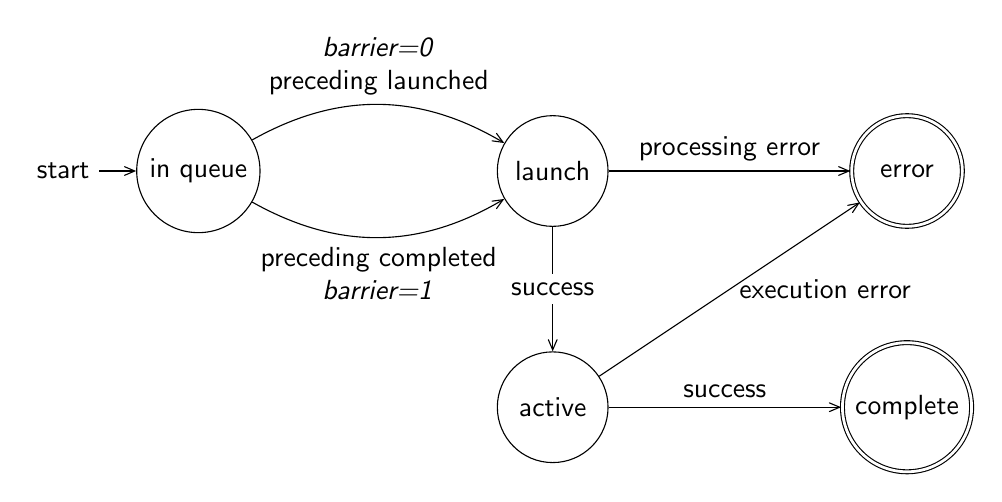
\begin{tikzpicture}
[auto,on grid,node distance=4.5cm,state/.style={circle,draw,minimum size=40pt}]
   \node[state,initial]                 (s0) {in queue};
   \node[state,right=4.5cm of s0]       (s1) {launch};
   \node[state,below=3cm of s1]       (s2) {active};
   \node[state,accepting,double distance=1pt,right=of s1]   (s3) {error};
   \node[state,accepting,double distance=1pt,right=of s2]   (s4) {complete};
   \path[->]
     (s0) edge[bend right]  node[text width=3cm,align=center,below] {preceding completed\\\textit{barrier=1}} (s1)
          edge[bend left] node[text width=3cm,align=center,above]{\textit{barrier=0}\\preceding launched} (s1)
     (s1) edge  node {processing error} (s3)
          edge  node[anchor=center,fill=white,opacity=1] {success} (s2)
     (s2) edge  node{success} (s4)
          edge  node[right]{execution error} (s3)
     ;
\end{tikzpicture}
  \centering
  \caption{Packet State Diagram}
  \label{fig:packetstate}
\end{figure}

After submission, a packet can be in one of the following five states:
\emph{in queue}, \emph{launch}, \emph{error}, \emph{active} or
\emph{complete}. Figure~\ref{fig:packetstate} shows the state transition
diagram.

\begin{description}[itemsep=2pt,leftmargin=0cm, labelindent=0cm] \item[In queue]
  The packet processor has not started to parse the current packet. If the
  barrier bit is set in the header, the transition to the launch state occurs
  only after all the preceding packets have completed their execution. If the
  barrier bit is not set, the transition occurs after the preceding packets have
  finished their launch phase.  In other words, while the packet processor is
  required to launch any consecutive two packets in order, it is not required to
  complete them in order unless the barrier bit of the second packet is set.

\item[Launch] The packet is being parsed, but it has not started execution. This
  phase finalizes by applying an acquire memory fence with the scope indicated
  by the acquire fence scope field in the header. Memory fences are explained
  in~\cite{prm}, Section 6.2.6.

  If an error is detected during launch, the queue transitions to the error
  state and the event callback associated with the queue (if present) is
  invoked. The runtime passes a status code to the callback that indicates the
  source of the problem.  The following status codes can be returned:
  \begin{description}[itemsep=1.5pt,labelindent=.5cm]
  \item[\hsaref{HSA_STATUS_ERROR_INVALID_PACKET_FORMAT}] Malformed AQL
    packet. This can happen if, for example, the packet header type is invalid.
  \item[\hsaref{HSA_STATUS_ERROR_OUT_OF_RESOURCES}] The packet processor is
    unable to allocate the resources required by the launch. This can happen
    if, for example, a kernel dispatch packet requests more group memory than
    the size of the group memory declared by the corresponding kernel agent.
  \end{description}
\item[Active] The execution of the packet has started.

  If an error is detected during this phase, the queue transitions to the error
  state, a release fence is applied to the packet with the scope indicated by
  the release fence scope field in the header, and the HSA runtime invokes the
  application callback associated with the queue. The following status codes can
  be returned:
  \begin{description}[itemsep=1.5pt,labelindent=.5cm]
  \item[\hsaref{HSA_STATUS_ERROR_EXCEPTION}] An HSAIL exception has been
    triggered during the execution of a kernel dispatch packet. For example, a
    floating point operation has resulted in an overflow.
  \end{description}

  If no error is detected, the transition to the complete state happens when the
  associated task finishes (in the case of kernel dispatch and agent dispatch
  packets), or when the dependencies are satisfied (in the case of a barrier-AND
  and barrier-OR packets).

\item[Complete] A memory release fence is applied with the scope indicated by
  the release fence scope field in the header, and the completion signal (if
  present) decremented.

\item[Error] An error was encountered during the launch or active phases. No
  further packets will be launched on the queue. The queue cannot be recovered,
  but only inactivated or destroyed. If the application passes the queue as an
  argument to any HSA function other than \hsaref{hsa_queue_inactivate} or
  \hsaref{hsa_queue_destroy}, the behavior is undefined.

\end{description}


\subsection{API}
\makeatletter{}

\subsubsection{hsa_\-packet_\-type_\-t}
\vspace{-2.5mm}Packet type.\begin{mylongtable}{@{}p{\textwidth}}
\rule{0pt}{3ex}typedef enum \{\\\hspace{1.7em}\hypertarget{group__aql_1gga35a04bfe654a1c980ac904cafd6373a1a86eecc1851fdf8b10538f994549ded8b}{\refenu{HSA_\-PACKET_\-TYPE_\-VENDOR_\-SPECIFIC}} = 0,\\
\hspace{1.7em}\hypertarget{group__aql_1gga35a04bfe654a1c980ac904cafd6373a1a9030931b8fe80fb9add8c796cd8886c5}{\refenu{HSA_\-PACKET_\-TYPE_\-INVALID}} = 1,\\
\hspace{1.7em}\hypertarget{group__aql_1gga35a04bfe654a1c980ac904cafd6373a1ab639dc86e45ee0c9d07022a2e79cab56}{\refenu{HSA_\-PACKET_\-TYPE_\-KERNEL_\-DISPATCH}} = 2,\\
\hspace{1.7em}\hypertarget{group__aql_1gga35a04bfe654a1c980ac904cafd6373a1a015bb0b76eccde0f58f27a570ada6b56}{\refenu{HSA_\-PACKET_\-TYPE_\-BARRIER_\-AND}} = 3,\\
\hspace{1.7em}\hypertarget{group__aql_1gga35a04bfe654a1c980ac904cafd6373a1aeb8ddfcceb12c29b12f52609e7bb7ce2}{\refenu{HSA_\-PACKET_\-TYPE_\-AGENT_\-DISPATCH}} = 4,\\
\hspace{1.7em}\hypertarget{group__aql_1gga35a04bfe654a1c980ac904cafd6373a1a1953e793495a0d122be19580cd6a2523}{\refenu{HSA_\-PACKET_\-TYPE_\-BARRIER_\-OR}} = 5\\
\} \hypertarget{group__aql_1ga35a04bfe654a1c980ac904cafd6373a1}{\textbf{hsa_\-packet_\-type_\-t}};\rule[-2ex]{0pt}{0pt}\end{mylongtable}\noindent\textbf{Values}\\[-7mm]
\begin{longtable}{@{\hspace{2em}}p{\linewidth-2em}}
\hspace{-2em}\refenu{HSA_\-PACKET_\-TYPE_\-VENDOR_\-SPECIFIC}\\Vendor-specific packet.\\[2mm]
\hspace{-2em}\refenu{HSA_\-PACKET_\-TYPE_\-INVALID}\\The packet has been processed in the past, but has not been reassigned to the packet processor. A packet processor must not process a packet of this type. All queues support this packet type.\\[2mm]
\hspace{-2em}\refenu{HSA_\-PACKET_\-TYPE_\-KERNEL_\-DISPATCH}\\Packet used by agents for dispatching jobs to kernel agents. Not all queues support packets of this type (see \hyperlink{group__queue_1ga1145b01f6d9e2670179a22c92db39413}{hsa_\-queue_\-feature_\-t}).\\[2mm]
\hspace{-2em}\refenu{HSA_\-PACKET_\-TYPE_\-BARRIER_\-AND}\\Packet used by agents to delay processing of subsequent packets, and to express complex dependencies between multiple packets. All queues support this packet type.\\[2mm]
\hspace{-2em}\refenu{HSA_\-PACKET_\-TYPE_\-AGENT_\-DISPATCH}\\Packet used by agents for dispatching jobs to agents. Not all queues support packets of this type (see \hyperlink{group__queue_1ga1145b01f6d9e2670179a22c92db39413}{hsa_\-queue_\-feature_\-t}).\\[2mm]
\hspace{-2em}\refenu{HSA_\-PACKET_\-TYPE_\-BARRIER_\-OR}\\Packet used by agents to delay processing of subsequent packets, and to express complex dependencies between multiple packets. All queues support this packet type.
\end{longtable}

\subsubsection{hsa_\-fence_\-scope_\-t}
\vspace{-2.5mm}Scope of the memory fence operation associated with a packet.\begin{mylongtable}{@{}p{\textwidth}}
\rule{0pt}{3ex}typedef enum \{\\\hspace{1.7em}\hypertarget{group__aql_1gga6c1a86878de5b0f980202ad7e4e8d42aa5dc7b942cd56f91094a088435027be2c}{\refenu{HSA_\-FENCE_\-SCOPE_\-NONE}} = 0,\\
\hspace{1.7em}\hypertarget{group__aql_1gga6c1a86878de5b0f980202ad7e4e8d42aa9879cf99ba63616fe61da22281df814e}{\refenu{HSA_\-FENCE_\-SCOPE_\-AGENT}} = 1,\\
\hspace{1.7em}\hypertarget{group__aql_1gga6c1a86878de5b0f980202ad7e4e8d42aa6ecb203c10f12ec4bcf475d527c3a870}{\refenu{HSA_\-FENCE_\-SCOPE_\-SYSTEM}} = 2\\
\} \hypertarget{group__aql_1ga6c1a86878de5b0f980202ad7e4e8d42a}{\textbf{hsa_\-fence_\-scope_\-t}};\rule[-2ex]{0pt}{0pt}\end{mylongtable}\noindent\textbf{Values}\\[-7mm]
\begin{longtable}{@{\hspace{2em}}p{\linewidth-2em}}
\hspace{-2em}\refenu{HSA_\-FENCE_\-SCOPE_\-NONE}\\No scope (no fence is applied). The packet relies on external fences to ensure visibility of memory updates.\\[2mm]
\hspace{-2em}\refenu{HSA_\-FENCE_\-SCOPE_\-AGENT}\\The fence is applied with agent scope for the global segment.\\[2mm]
\hspace{-2em}\refenu{HSA_\-FENCE_\-SCOPE_\-SYSTEM}\\The fence is applied across both agent and system scope for the global segment.
\end{longtable}

\subsubsection{hsa_\-packet_\-header_\-t}
\vspace{-2.5mm}Sub-fields of the \textit{header} field that is present in any AQL packet. The offset (with respect to the address of \textit{header}) of a sub-field is identical to its enumeration constant. The width of each sub-field is determined by the corresponding value in \hyperlink{group__aql_1gad1d46c8ae53112cb06bf364b65b4b0ca}{hsa_\-packet_\-header_\-width_\-t}. The offset and the width are expressed in bits.\begin{mylongtable}{@{}p{\textwidth}}
\rule{0pt}{3ex}typedef enum \{\\\hspace{1.7em}\hypertarget{group__aql_1gga2f03beef9c37e464b3837f2646d30870a28b2f227c66db4ddcefb5856e7958e6c}{\refenu{HSA_\-PACKET_\-HEADER_\-TYPE}} = 0,\\
\hspace{1.7em}\hypertarget{group__aql_1gga2f03beef9c37e464b3837f2646d30870aa967f75e5d6ad03f764a1db4bb8351a4}{\refenu{HSA_\-PACKET_\-HEADER_\-BARRIER}} = 8,\\
\hspace{1.7em}\hypertarget{group__aql_1gga2f03beef9c37e464b3837f2646d30870a02bc578de13a9abc0d2ba7f59e788960}{\refenu{HSA_\-PACKET_\-HEADER_\-SCACQUIRE_\-FENCE_\-SCOPE}} = 9,\\
\hspace{1.7em}\hypertarget{group__aql_1gga2f03beef9c37e464b3837f2646d30870a8fd59e5972b701019cb4b55799891ced}{\refenu{HSA_\-PACKET_\-HEADER_\-SCRELEASE_\-FENCE_\-SCOPE}} = 11\\
\} \hypertarget{group__aql_1ga2f03beef9c37e464b3837f2646d30870}{\textbf{hsa_\-packet_\-header_\-t}};\rule[-2ex]{0pt}{0pt}\end{mylongtable}\noindent\textbf{Values}\\[-7mm]
\begin{longtable}{@{\hspace{2em}}p{\linewidth-2em}}
\hspace{-2em}\refenu{HSA_\-PACKET_\-HEADER_\-TYPE}\\Packet type. The value of this sub-field must be one of \hyperlink{group__aql_1ga35a04bfe654a1c980ac904cafd6373a1}{hsa_\-packet_\-type_\-t}. If the type is \hyperlink{group__aql_1gga35a04bfe654a1c980ac904cafd6373a1a86eecc1851fdf8b10538f994549ded8b}{HSA_\-PACKET_\-TYPE_\-VENDOR_\-SPECIFIC}, the packet layout is vendor-specific.\\[2mm]
\hspace{-2em}\refenu{HSA_\-PACKET_\-HEADER_\-BARRIER}\\Barrier bit. If the barrier bit is set, the processing of the current packet only launches when all preceding packets (within the same queue) are complete.\\[2mm]
\hspace{-2em}\refenu{HSA_\-PACKET_\-HEADER_\-SCACQUIRE_\-FENCE_\-SCOPE}\\Acquire fence scope. The value of this sub-field determines the scope and type of the memory fence operation applied before the packet enters the active phase. An acquire fence ensures that any subsequent global segment or image loads by any unit of execution that belongs to a dispatch that has not yet entered the active phase on any queue of the same kernel agent, sees any data previously released at the scopes specified by the acquire fence. The value of this sub-field must be one of \hyperlink{group__aql_1ga6c1a86878de5b0f980202ad7e4e8d42a}{hsa_\-fence_\-scope_\-t}.\\[2mm]
\hspace{-2em}\refenu{HSA_\-PACKET_\-HEADER_\-SCRELEASE_\-FENCE_\-SCOPE}\\Release fence scope, The value of this sub-field determines the scope and type of the memory fence operation applied after kernel completion but before the packet is completed. A release fence makes any global segment or image data that was stored by any unit of execution that belonged to a dispatch that has completed the active phase on any queue of the same kernel agent visible in all the scopes specified by the release fence. The value of this sub-field must be one of \hyperlink{group__aql_1ga6c1a86878de5b0f980202ad7e4e8d42a}{hsa_\-fence_\-scope_\-t}.
\end{longtable}

\subsubsection{hsa_\-packet_\-header_\-width_\-t}
\vspace{-2.5mm}Width (in bits) of the sub-fields in \hyperlink{group__aql_1ga2f03beef9c37e464b3837f2646d30870}{hsa_\-packet_\-header_\-t}.\begin{mylongtable}{@{}p{\textwidth}}
\rule{0pt}{3ex}typedef enum \{\\\hspace{1.7em}\hypertarget{group__aql_1ggad1d46c8ae53112cb06bf364b65b4b0caa9d692b0ccc6dcf9fa2f8fe908d0f5f5e}{\refenu{HSA_\-PACKET_\-HEADER_\-WIDTH_\-TYPE}} = 8,\\
\hspace{1.7em}\hypertarget{group__aql_1ggad1d46c8ae53112cb06bf364b65b4b0caa66f1ecb4b8877e84ae33ecf0d9696453}{\refenu{HSA_\-PACKET_\-HEADER_\-WIDTH_\-BARRIER}} = 1,\\
\hspace{1.7em}\hypertarget{group__aql_1ggad1d46c8ae53112cb06bf364b65b4b0caa57349a3d0d98ddd32020ff5269916704}{\refenu{HSA_\-PACKET_\-HEADER_\-WIDTH_\-SCACQUIRE_\-FENCE_\-SCOPE}} = 2,\\
\hspace{1.7em}\hypertarget{group__aql_1ggad1d46c8ae53112cb06bf364b65b4b0caa073e6f770ee5da8322269dce0b09977c}{\refenu{HSA_\-PACKET_\-HEADER_\-WIDTH_\-SCRELEASE_\-FENCE_\-SCOPE}} = 2\\
\} \hypertarget{group__aql_1gad1d46c8ae53112cb06bf364b65b4b0ca}{\textbf{hsa_\-packet_\-header_\-width_\-t}};\rule[-2ex]{0pt}{0pt}\end{mylongtable}\noindent\textbf{Values}\\[-7mm]
\begin{longtable}{@{\hspace{2em}}p{\linewidth-2em}}
\hspace{-2em}\refenu{HSA_\-PACKET_\-HEADER_\-WIDTH_\-TYPE}\\[2mm]
\hspace{-2em}\refenu{HSA_\-PACKET_\-HEADER_\-WIDTH_\-BARRIER}\\[2mm]
\hspace{-2em}\refenu{HSA_\-PACKET_\-HEADER_\-WIDTH_\-SCACQUIRE_\-FENCE_\-SCOPE}\\[2mm]
\hspace{-2em}\refenu{HSA_\-PACKET_\-HEADER_\-WIDTH_\-SCRELEASE_\-FENCE_\-SCOPE}
\end{longtable}

\subsubsection{hsa_\-kernel_\-dispatch_\-packet_\-setup_\-t}
\vspace{-2.5mm}Sub-fields of the kernel dispatch packet \textit{setup} field. The offset (with respect to the address of \textit{setup}) of a sub-field is identical to its enumeration constant. The width of each sub-field is determined by the corresponding value in \hyperlink{group__aql_1gacf1c0ae7598d222c582cf5f68aefc994}{hsa_\-kernel_\-dispatch_\-packet_\-setup_\-width_\-t}. The offset and the width are expressed in bits.\begin{mylongtable}{@{}p{\textwidth}}
\rule{0pt}{3ex}typedef enum \{\\\hspace{1.7em}\hypertarget{group__aql_1gga0b4e16703a05220bbd72a70bb0fca6faa7fbd464fd82b46169843e11877f60bde}{\refenu{HSA_\-KERNEL_\-DISPATCH_\-PACKET_\-SETUP_\-DIMENSIONS}} = 0\\
\} \hypertarget{group__aql_1ga0b4e16703a05220bbd72a70bb0fca6fa}{\textbf{hsa_\-kernel_\-dispatch_\-packet_\-setup_\-t}};\rule[-2ex]{0pt}{0pt}\end{mylongtable}\noindent\textbf{Values}\\[-7mm]
\begin{longtable}{@{\hspace{2em}}p{\linewidth-2em}}
\hspace{-2em}\refenu{HSA_\-KERNEL_\-DISPATCH_\-PACKET_\-SETUP_\-DIMENSIONS}\\Number of dimensions of the grid. Valid values are 1, 2, or 3.
\end{longtable}

\subsubsection{hsa_\-kernel_\-dispatch_\-packet_\-setup_\-width_\-t}
\vspace{-2.5mm}Width (in bits) of the sub-fields in \hyperlink{group__aql_1ga0b4e16703a05220bbd72a70bb0fca6fa}{hsa_\-kernel_\-dispatch_\-packet_\-setup_\-t}.\begin{mylongtable}{@{}p{\textwidth}}
\rule{0pt}{3ex}typedef enum \{\\\hspace{1.7em}\hypertarget{group__aql_1ggacf1c0ae7598d222c582cf5f68aefc994a8eae1a35c31d2e0295bfaf3c15f03c79}{\refenu{HSA_\-KERNEL_\-DISPATCH_\-PACKET_\-SETUP_\-WIDTH_\-DIMENSIONS}} = 2\\
\} \hypertarget{group__aql_1gacf1c0ae7598d222c582cf5f68aefc994}{\textbf{hsa_\-kernel_\-dispatch_\-packet_\-setup_\-width_\-t}};\rule[-2ex]{0pt}{0pt}\end{mylongtable}

\subsubsection{hsa_\-kernel_\-dispatch_\-packet_\-t}
\vspace{-2.5mm}AQL kernel dispatch packet.\begin{mylongtable}{@{}p{\textwidth}}
\rule{0pt}{3ex}typedef struct  hsa_kernel_dispatch_packet_s \{\\
\hspace{1.7em}uint16_\-t \reffld{header};\\
\hspace{1.7em}uint16_\-t \reffld{setup};\\
\hspace{1.7em}uint16_\-t \reffld{workgroup_\-size_\-x};\\
\hspace{1.7em}uint16_\-t \reffld{workgroup_\-size_\-y};\\
\hspace{1.7em}uint16_\-t \reffld{workgroup_\-size_\-z};\\
\hspace{1.7em}uint16_\-t \reffld{reserved0};\\
\hspace{1.7em}uint32_\-t \reffld{grid_\-size_\-x};\\
\hspace{1.7em}uint32_\-t \reffld{grid_\-size_\-y};\\
\hspace{1.7em}uint32_\-t \reffld{grid_\-size_\-z};\\
\hspace{1.7em}uint32_\-t \reffld{private_\-segment_\-size};\\
\hspace{1.7em}uint32_\-t \reffld{group_\-segment_\-size};\\
\hspace{1.7em}uint64_\-t \reffld{kernel_\-object};\\
\\[-2mm]\#ifdef HSA_LARGE_MODEL\\\hspace{1.7em}void * \reffld{kernarg_\-address};\\
\#elif  defined HSA_LITTLE_ENDIAN\\\hspace{1.7em}void * \reffld{kernarg_\-address};\\
\hspace{1.7em}uint32_\-t \reffld{reserved1};\\
\#else\\\hspace{1.7em}uint32_\-t \reffld{reserved1};\\
\hspace{1.7em}void * \reffld{kernarg_\-address};\\
\#endif\\[2mm]\hspace{1.7em}uint64_\-t \reffld{reserved2};\\
\hspace{1.7em}\hyperlink{group__signals_1ga63e0b9e11f9d4f51a2f3a9bfaee9ad99}{hsa_\-signal_\-t} \reffld{completion_\-signal};\\
\}  \hypertarget{group__aql_1ga408b6584508e94b96038693f9eaea75d}{\textbf{hsa_\-kernel_\-dispatch_\-packet_\-t}}\rule[-2ex]{0pt}{0pt}
\end{mylongtable}

\noindent\textbf{Data Fields}\\[-7mm]
\begin{longtable}{@{}>{\hangindent=2em}p{\textwidth}}
\hypertarget{hsa_\-kernel_\-dispatch_\-packet_\-t.header}{\reffld{header}}\\\hspace{2em}Packet header. Used to configure multiple packet parameters such as the packet type. The parameters are described by \hyperlink{group__aql_1ga2f03beef9c37e464b3837f2646d30870}{hsa_\-packet_\-header_\-t}.\\[2mm]
\hypertarget{hsa_\-kernel_\-dispatch_\-packet_\-t.setup}{\reffld{setup}}\\\hspace{2em}Dispatch setup parameters. Used to configure kernel dispatch parameters such as the number of dimensions in the grid. The parameters are described by \hyperlink{group__aql_1ga0b4e16703a05220bbd72a70bb0fca6fa}{hsa_\-kernel_\-dispatch_\-packet_\-setup_\-t}.\\[2mm]
\hypertarget{hsa_\-kernel_\-dispatch_\-packet_\-t.workgroup_\-size_\-x}{\reffld{workgroup_\-size_\-x}}\\\hspace{2em}X dimension of work-group, in work-items. Must be greater than 0.\\[2mm]
\hypertarget{hsa_\-kernel_\-dispatch_\-packet_\-t.workgroup_\-size_\-y}{\reffld{workgroup_\-size_\-y}}\\\hspace{2em}Y dimension of work-group, in work-items. Must be greater than 0. If the grid has 1 dimension, the only valid value is 1.\\[2mm]
\hypertarget{hsa_\-kernel_\-dispatch_\-packet_\-t.workgroup_\-size_\-z}{\reffld{workgroup_\-size_\-z}}\\\hspace{2em}Z dimension of work-group, in work-items. Must be greater than 0. If the grid has 1 or 2 dimensions, the only valid value is 1.\\[2mm]
\hypertarget{hsa_\-kernel_\-dispatch_\-packet_\-t.reserved0}{\reffld{reserved0}}\\\hspace{2em}Reserved. Must be 0.\\[2mm]
\hypertarget{hsa_\-kernel_\-dispatch_\-packet_\-t.grid_\-size_\-x}{\reffld{grid_\-size_\-x}}\\\hspace{2em}X dimension of grid, in work-items. Must be greater than 0. Must not be smaller than \textit{workgroup_\-size_\-x}.\\[2mm]
\hypertarget{hsa_\-kernel_\-dispatch_\-packet_\-t.grid_\-size_\-y}{\reffld{grid_\-size_\-y}}\\\hspace{2em}Y dimension of grid, in work-items. Must be greater than 0. If the grid has 1 dimension, the only valid value is 1. Must not be smaller than \textit{workgroup_\-size_\-y}.\\[2mm]
\hypertarget{hsa_\-kernel_\-dispatch_\-packet_\-t.grid_\-size_\-z}{\reffld{grid_\-size_\-z}}\\\hspace{2em}Z dimension of grid, in work-items. Must be greater than 0. If the grid has 1 or 2 dimensions, the only valid value is 1. Must not be smaller than \textit{workgroup_\-size_\-z}.\\[2mm]
\hypertarget{hsa_\-kernel_\-dispatch_\-packet_\-t.private_\-segment_\-size}{\reffld{private_\-segment_\-size}}\\\hspace{2em}Size in bytes of private memory allocation request (per work-item).\\[2mm]
\hypertarget{hsa_\-kernel_\-dispatch_\-packet_\-t.group_\-segment_\-size}{\reffld{group_\-segment_\-size}}\\\hspace{2em}Size in bytes of group memory allocation request (per work-group). Must not be less than the sum of the group memory used by the kernel (and the functions it calls directly or indirectly) and the dynamically allocated group segment variables.\\[2mm]
\hypertarget{hsa_\-kernel_\-dispatch_\-packet_\-t.kernel_\-object}{\reffld{kernel_\-object}}\\\hspace{2em}Opaque handle to a code object that includes an implementation-defined executable code for the kernel.\\[2mm]
\hypertarget{hsa_\-kernel_\-dispatch_\-packet_\-t.kernarg_\-address}{\reffld{kernarg_\-address}}\\\hspace{2em}Pointer to a buffer containing the kernel arguments. May be NULL.\\[1.25mm]
\hspace{2em}The buffer must be allocated using \hyperlink{group__memory_1ga39f7943b93aa2bb754726fc74d929426}{\reffun{hsa_\-memory_\-allocate}}, and must not be modified once the kernel dispatch packet is enqueued until the dispatch has completed execution.\\[2mm]
\hypertarget{hsa_\-kernel_\-dispatch_\-packet_\-t.reserved1}{\reffld{reserved1}}\\\hspace{2em}Reserved. Must be 0.\\[2mm]
\hypertarget{hsa_\-kernel_\-dispatch_\-packet_\-t.reserved2}{\reffld{reserved2}}\\\hspace{2em}Reserved. Must be 0.\\[2mm]
\hypertarget{hsa_\-kernel_\-dispatch_\-packet_\-t.completion_\-signal}{\reffld{completion_\-signal}}\\\hspace{2em}Signal used to indicate completion of the job. The application can use the special signal handle 0 to indicate that no signal is used.
\end{longtable}



\subsubsection{hsa_\-agent_\-dispatch_\-packet_\-t}
\vspace{-2.5mm}Agent dispatch packet.\begin{mylongtable}{@{}p{\textwidth}}
\rule{0pt}{3ex}typedef struct  hsa_agent_dispatch_packet_s \{\\
\hspace{1.7em}uint16_\-t \reffld{header};\\
\hspace{1.7em}uint16_\-t \reffld{type};\\
\hspace{1.7em}uint32_\-t \reffld{reserved0};\\
\\[-2mm]\#ifdef HSA_LARGE_MODEL\\\hspace{1.7em}void * \reffld{return_\-address};\\
\#elif  defined HSA_LITTLE_ENDIAN\\\hspace{1.7em}void * \reffld{return_\-address};\\
\hspace{1.7em}uint32_\-t \reffld{reserved1};\\
\#else\\\hspace{1.7em}uint32_\-t \reffld{reserved1};\\
\hspace{1.7em}void * \reffld{return_\-address};\\
\#endif\\[2mm]\hspace{1.7em}uint64_\-t \reffld{arg}[4];\\
\hspace{1.7em}uint64_\-t \reffld{reserved2};\\
\hspace{1.7em}\hyperlink{group__signals_1ga63e0b9e11f9d4f51a2f3a9bfaee9ad99}{hsa_\-signal_\-t} \reffld{completion_\-signal};\\
\}  \hypertarget{group__aql_1gaf1fa68d31bcdc7c0eb772e11179520b8}{\textbf{hsa_\-agent_\-dispatch_\-packet_\-t}}\rule[-2ex]{0pt}{0pt}
\end{mylongtable}

\noindent\textbf{Data Fields}\\[-7mm]
\begin{longtable}{@{}>{\hangindent=2em}p{\textwidth}}
\hypertarget{hsa_\-agent_\-dispatch_\-packet_\-t.header}{\reffld{header}}\\\hspace{2em}Packet header. Used to configure multiple packet parameters such as the packet type. The parameters are described by \hyperlink{group__aql_1ga2f03beef9c37e464b3837f2646d30870}{hsa_\-packet_\-header_\-t}.\\[2mm]
\hypertarget{hsa_\-agent_\-dispatch_\-packet_\-t.type}{\reffld{type}}\\\hspace{2em}Application-defined function to be performed by the destination agent.\\[2mm]
\hypertarget{hsa_\-agent_\-dispatch_\-packet_\-t.reserved0}{\reffld{reserved0}}\\\hspace{2em}Reserved. Must be 0.\\[2mm]
\hypertarget{hsa_\-agent_\-dispatch_\-packet_\-t.return_\-address}{\reffld{return_\-address}}\\\hspace{2em}Address where to store the function return values, if any.\\[2mm]
\hypertarget{hsa_\-agent_\-dispatch_\-packet_\-t.reserved1}{\reffld{reserved1}}\\\hspace{2em}Reserved. Must be 0.\\[2mm]
\hypertarget{hsa_\-agent_\-dispatch_\-packet_\-t.arg}{\reffld{arg}}\\\hspace{2em}Function arguments.\\[2mm]
\hypertarget{hsa_\-agent_\-dispatch_\-packet_\-t.reserved2}{\reffld{reserved2}}\\\hspace{2em}Reserved. Must be 0.\\[2mm]
\hypertarget{hsa_\-agent_\-dispatch_\-packet_\-t.completion_\-signal}{\reffld{completion_\-signal}}\\\hspace{2em}Signal used to indicate completion of the job. The application can use the special signal handle 0 to indicate that no signal is used.
\end{longtable}



\subsubsection{hsa_\-barrier_\-and_\-packet_\-t}
\vspace{-2.5mm}Barrier-AND packet.\begin{mylongtable}{@{}p{\textwidth}}
\rule{0pt}{3ex}typedef struct  hsa_barrier_and_packet_s \{\\
\hspace{1.7em}uint16_\-t \reffld{header};\\
\hspace{1.7em}uint16_\-t \reffld{reserved0};\\
\hspace{1.7em}uint32_\-t \reffld{reserved1};\\
\hspace{1.7em}\hyperlink{group__signals_1ga63e0b9e11f9d4f51a2f3a9bfaee9ad99}{hsa_\-signal_\-t} \reffld{dep_\-signal}[5];\\
\hspace{1.7em}uint64_\-t \reffld{reserved2};\\
\hspace{1.7em}\hyperlink{group__signals_1ga63e0b9e11f9d4f51a2f3a9bfaee9ad99}{hsa_\-signal_\-t} \reffld{completion_\-signal};\\
\}  \hypertarget{group__aql_1ga28086c03590c7715cd9f421de7b9fe34}{\textbf{hsa_\-barrier_\-and_\-packet_\-t}}\rule[-2ex]{0pt}{0pt}
\end{mylongtable}

\noindent\textbf{Data Fields}\\[-7mm]
\begin{longtable}{@{}>{\hangindent=2em}p{\textwidth}}
\hypertarget{hsa_\-barrier_\-and_\-packet_\-t.header}{\reffld{header}}\\\hspace{2em}Packet header. Used to configure multiple packet parameters such as the packet type. The parameters are described by \hyperlink{group__aql_1ga2f03beef9c37e464b3837f2646d30870}{hsa_\-packet_\-header_\-t}.\\[2mm]
\hypertarget{hsa_\-barrier_\-and_\-packet_\-t.reserved0}{\reffld{reserved0}}\\\hspace{2em}Reserved. Must be 0.\\[2mm]
\hypertarget{hsa_\-barrier_\-and_\-packet_\-t.reserved1}{\reffld{reserved1}}\\\hspace{2em}Reserved. Must be 0.\\[2mm]
\hypertarget{hsa_\-barrier_\-and_\-packet_\-t.dep_\-signal}{\reffld{dep_\-signal}}\\\hspace{2em}Array of dependent signal objects. Signals with a handle value of 0 are allowed and are interpreted by the packet processor as satisfied dependencies.\\[2mm]
\hypertarget{hsa_\-barrier_\-and_\-packet_\-t.reserved2}{\reffld{reserved2}}\\\hspace{2em}Reserved. Must be 0.\\[2mm]
\hypertarget{hsa_\-barrier_\-and_\-packet_\-t.completion_\-signal}{\reffld{completion_\-signal}}\\\hspace{2em}Signal used to indicate completion of the job. The application can use the special signal handle 0 to indicate that no signal is used.
\end{longtable}



\subsubsection{hsa_\-barrier_\-or_\-packet_\-t}
\vspace{-2.5mm}Barrier-OR packet.\begin{mylongtable}{@{}p{\textwidth}}
\rule{0pt}{3ex}typedef struct  hsa_barrier_or_packet_s \{\\
\hspace{1.7em}uint16_\-t \reffld{header};\\
\hspace{1.7em}uint16_\-t \reffld{reserved0};\\
\hspace{1.7em}uint32_\-t \reffld{reserved1};\\
\hspace{1.7em}\hyperlink{group__signals_1ga63e0b9e11f9d4f51a2f3a9bfaee9ad99}{hsa_\-signal_\-t} \reffld{dep_\-signal}[5];\\
\hspace{1.7em}uint64_\-t \reffld{reserved2};\\
\hspace{1.7em}\hyperlink{group__signals_1ga63e0b9e11f9d4f51a2f3a9bfaee9ad99}{hsa_\-signal_\-t} \reffld{completion_\-signal};\\
\}  \hypertarget{group__aql_1ga69e646654b0f2fb7a7ad0388851afe7b}{\textbf{hsa_\-barrier_\-or_\-packet_\-t}}\rule[-2ex]{0pt}{0pt}
\end{mylongtable}

\noindent\textbf{Data Fields}\\[-7mm]
\begin{longtable}{@{}>{\hangindent=2em}p{\textwidth}}
\hypertarget{hsa_\-barrier_\-or_\-packet_\-t.header}{\reffld{header}}\\\hspace{2em}Packet header. Used to configure multiple packet parameters such as the packet type. The parameters are described by \hyperlink{group__aql_1ga2f03beef9c37e464b3837f2646d30870}{hsa_\-packet_\-header_\-t}.\\[2mm]
\hypertarget{hsa_\-barrier_\-or_\-packet_\-t.reserved0}{\reffld{reserved0}}\\\hspace{2em}Reserved. Must be 0.\\[2mm]
\hypertarget{hsa_\-barrier_\-or_\-packet_\-t.reserved1}{\reffld{reserved1}}\\\hspace{2em}Reserved. Must be 0.\\[2mm]
\hypertarget{hsa_\-barrier_\-or_\-packet_\-t.dep_\-signal}{\reffld{dep_\-signal}}\\\hspace{2em}Array of dependent signal objects. Signals with a handle value of 0 are allowed and are interpreted by the packet processor as dependencies not satisfied.\\[2mm]
\hypertarget{hsa_\-barrier_\-or_\-packet_\-t.reserved2}{\reffld{reserved2}}\\\hspace{2em}Reserved. Must be 0.\\[2mm]
\hypertarget{hsa_\-barrier_\-or_\-packet_\-t.completion_\-signal}{\reffld{completion_\-signal}}\\\hspace{2em}Signal used to indicate completion of the job. The application can use the special signal handle 0 to indicate that no signal is used.
\end{longtable}

 

\section{Memory}\label{sec:memory}

The HSA runtime API provides a compact set of functions for inspecting the
memory \emph{regions} that are accessible from an agent, and (if applicable)
allocating memory on those regions.

A memory region represents a block of virtual memory with certain
characteristics that is accessible by one or more agents. The region object
\hsaref{hsa_region_t} exposes properties about the block of memory such as the
associated memory segment, size, and in some cases allocation characteristics.

The function \hsaref{hsa_agent_iterate_regions} can be used to inspect the set
of regions associated with an agent.  If the application can allocate memory
in a region using the function \hsaref{hsa_memory_allocate}, the flag
\hsaref{HSA_REGION_INFO_RUNTIME_ALLOC_ALLOWED} is set for that region. The HSA
runtime allocator can only be used to allocate memory in the global and readonly
segments. Memory in the private, group and kernarg segments is automatically
allocated when a kernel dispatch packet is launched.

When the application no longer needs a buffer that was allocated with the
function \hsaref{hsa_memory_allocate}, it invokes \hsaref{hsa_memory_free} to
release the memory. The application shall not release a runtime-allocated buffer
using standard libraries (such as the function free). Conversely, the runtime
deallocator cannot be used to release memory allocated using standard libraries
(such as the function malloc).

\subsection{Global memory}\label{sec:memory:global}

Regions associated with the global segment are divided into two broad
categories: fine-grained and coarse-grained. The main difference between these
memory types is that fine-grained memory is directly accessible to all the
agents in the system at the same time (under the terms of the HSA memory model),
while coarse-grained memory may be accessible to multiple agents, but never at
the same time: the application is responsible for explicitly assigning ownership
of a buffer to a specific agent. In addition to this, the application can only
use memory allocated from a fine-grained region in order to pass arguments to a
kernel, but not all fine-grained regions can be used for this purpose.

Implementations of the HSA runtime are required to report at least the following
fine-grained regions on every HSA system:
\begin{itemize}[itemsep=1pt,topsep=3pt,partopsep=0pt]
\item A fine-grained region that is located in the global segment and
  corresponds to the coherent, primary HSA memory type~\cite{sar}. The value of
  the attribute \hsaref{HSA_REGION_INFO_SEGMENT} in this region is
  \hsaref{HSA_REGION_SEGMENT_GLOBAL}, and the
  \hsaref{HSA_REGION_GLOBAL_FLAG_FINE_GRAINED} flag must be set.
\item If the HSA system exposes at least one kernel agent, a fine-grained
  region that is located in the global segment and can be used to allocate
  backing storage for the kernarg segment:
  \hsaref{HSA_REGION_GLOBAL_FLAG_KERNARG} is true, and
  \hsaref{HSA_REGION_INFO_RUNTIME_ALLOC_ALLOWED} is true.
\end{itemize}

Memory allocated outside of the HSA API (for example, using malloc) is
considered fine-grained only for those agents in the system that support the
Full profile, but cannot be used to pass arguments to a kernel. In agents
that only support the Base profile, fine-grained semantics are constrained to
buffers allocated using \hsaref{hsa_memory_allocate}.

If a buffer allocated outside of the HSA API is accessed by a kernel agent
that supports the Full profile, the application is encouraged to \emph{register}
the corresponding address range beforehand using the
\hsaref{hsa_memory_register} function. While kernels running on kernel agents
with Full profile support can access any regular host pointer, a registered
buffer can result on improved access performance.  When the application no
longer needs to access a registered buffer, it should deregister that virtual
address range by invoking \hsaref{hsa_memory_deregister}.

Coarse-grained regions are visible to one or more agents. The application can
determine that a region supports coarse-grained semantics because the value of
the attribute \hsaref{HSA_REGION_INFO_SEGMENT} is
\hsaref{HSA_REGION_SEGMENT_GLOBAL}, and the
\hsaref{HSA_REGION_GLOBAL_FLAG_COARSE_GRAINED} flag is set. If the same region
handle is accessible to several agents, the application can explicitly transfer
the ownership of buffers allocated in that region to any of those agents, but
only one owner is allowed at a time. The HSA runtime exposes the function
\hsaref{hsa_memory_assign_agent} to assign ownership of a buffer to an agent. It
is important to note that:
\begin{itemize}[itemsep=1pt,topsep=3pt,partopsep=0pt]
\item The ownership change affects a buffer within a region, and not the entire
  region. Different buffers within the same coarse-grained region can have
  different owners.
\item If the new owner cannot access the region associated with the buffer, the
  behavior is undefined.
\item Ownership change is a no-op for fine-grained buffers.
\end{itemize}

When a coarse-grained region is visible to a unique agent (i.e., the region
is only reported by \hsaref{hsa_agent_iterate_regions} for that agent), the
application can only assign ownership of memory within the region to that same
agent. This particular case of coarse-grained memory is also know as agent
allocation~\cite{prm}. An application can still access the contents of an agent
allocation buffer by invoking the synchronous copy function
(\hsaref{hsa_memory_copy}).

\subsubsection{Example: passing arguments to a kernel}\label{ex:kernarg_dispatch}
In the kernel setup example listed in Section~\ref{dispatch-packet}, the kernel
receives no arguments:
\begin{lstlisting}
packet->kernarg_address = NULL;
\end{lstlisting}
Let's assume now that the kernel expects a single argument, a signal handle. The
application needs to populate the
\hsaref{hsa_kernel_dispatch_packet_t.kernarg_address} field of the kernel
dispatch packet with the address of a buffer containing the signal.

The application searches for a memory region that can be used to allocate
backing storage for the kernarg segment. Once found, it reserves enough space to
hold the signal argument. While the actual amount of memory to be allocated is
determined by the finalizer, for simplicity we will assume that it matches the
size of a signal handle.
\begin{lstlisting}
hsa_region_t region;
hsa_agent_iterate_regions(kernel_agent, get_kernarg, &region);

// Allocate a buffer where to place the kernel arguments.
hsa_memory_allocate(region, sizeof(hsa_signal_t), (void**) &packet->kernarg_address);

// Place the signal the argument buffer
hsa_signal_t* buffer = (hsa_signal_t*) packet->kernarg_address;
assert(buffer != NULL);
hsa_signal_t signal;
hsa_signal_create(128, 1, &kernel_agent, &signal);
*buffer = signal;
\end{lstlisting}
The definition of \textit{get_kernarg} is:
\begin{lstlisting}
hsa_status_t get_kernarg(hsa_region_t region, void* data) {
    hsa_region_segment_t segment;
    hsa_region_get_info(region, HSA_REGION_INFO_SEGMENT, &segment);
    if (segment != HSA_REGION_SEGMENT_GLOBAL) {
        return HSA_STATUS_SUCCESS;
    }
    hsa_region_global_flag_t flags;
    hsa_region_get_info(region, HSA_REGION_INFO_GLOBAL_FLAGS, &flags);
    if (flags & HSA_REGION_GLOBAL_FLAG_KERNARG) {
        hsa_region_t* ret = (hsa_region_t*) data;
        *ret = region;
        return HSA_STATUS_INFO_BREAK;
    }
    return HSA_STATUS_SUCCESS;
}
\end{lstlisting}
The rest of the dispatch process remains the same.

\subsection{Readonly memory}
The application can allocate memory in a readonly region in order to store
information that remains constant during the execution of a kernel. Kernel
agents are only permitted to perform read operations on the addresses of
variables that reside in readonly memory.  The contents of a readonly buffer can
be initialized or changed from one kernel dispatch execution to another by the
application using the copy function (\hsaref{hsa_memory_copy}).

Each kernel agent exposes one or more readonly regions, which are private to
that kernel agent. Passing a readonly buffer associated with one agent in a
kernel dispatch packet that is executed to a different agent results in
undefined behavior.

Accesses to readonly buffers might perform better than accesses to global
buffers on some HSA implementations. All readonly memory is persistent across
the lifetime of an application.

\subsection{Group and Private memory}
Memory in the group segment is used to store information that is shared by all
the work-items in a work-group. Group memory is visible to the work-items of a
single work-group of a kernel dispatch. An address of a variable in group memory
can be read and written by any work-item in the work-group with which it is
associated, but not by work-items in other work-groups or by other agents. Group
memory is persistent across the execution of the work-items in the work-group of
the kernel dispatch with which it is associated, and it is uninitialized
when the work-group starts execution.

Memory in the private segment is used to store information local to a single
work-item. Private memory is visible only to a single work-item of a kernel
dispatch. An address of a variable in private memory can be read and written
only by the work-item with which it is associated, but not by any other
work-items or other agents.  Private memory is persistent across the execution
of the work-item with which it is associated, and it is uninitialized
when the work-item starts.

Memory in the group and private segments is represented in the HSA runtime API
in a similar fashion to memory in the global and readonly segments: using
regions. Each kernel agent exposes a group and a private regions. However, the
application is not allowed to explicitly allocate memory in these regions using
\hsaref{hsa_memory_allocate}, nor it can copy any contents into them using
\hsaref{hsa_memory_copy}. On the other hand, the application must specify the
amount of group and private memory that needs to be allocated for a particular
execution of a kernel, by populating the
\hsaref{hsa_kernel_dispatch_packet_t.group_segment_size} and
\hsaref{hsa_kernel_dispatch_packet_t.private_segment_size} fields of the kernel
dispatch packet.

The actual allocation of group and private memory happens automatically, before
a kernel starts execution. The application must ensure that the amount of group
memory requested per work-group does not exceed the maximum allocation size
declared by the kernel agent where the kernel dispatch packet is enqueued, which
is the value of the \hsaref{HSA_REGION_INFO_ALLOC_MAX_SIZE} attribute in the
group region associated with that kernel agent. Similarly, the private memory
usage of a kernel dispatch packet must not exceed the value of
\hsaref{HSA_REGION_INFO_ALLOC_MAX_SIZE} for the corresponding private region.

\subsection{API}
\makeatletter{}

\subsubsection{hsa_\-region_\-t}
\vspace{-2.5mm}A memory region represents a block of virtual memory with certain properties. For example, the HSA runtime represents fine-grained memory in the global segment using a region. A region might be associated with more than one agent.\begin{mylongtable}{@{}p{\textwidth}}
\rule{0pt}{3ex}typedef struct  hsa_region_s \{\\
\hspace{1.7em}uint64_\-t \reffld{handle};\\
\}  \hypertarget{group__memory_1gafa2782b67a8dd54814f07ba4f3dc29b5}{\textbf{hsa_\-region_\-t}}\rule[-2ex]{0pt}{0pt}
\end{mylongtable}

\noindent\textbf{Data Fields}\\[-7mm]
\begin{longtable}{@{}>{\hangindent=2em}p{\textwidth}}
\hypertarget{hsa_\-region_\-t.handle}{\reffld{handle}}\\\hspace{2em}Opaque handle.
\end{longtable}



\subsubsection{hsa_\-region_\-segment_\-t}
\vspace{-2.5mm}Memory segments associated with a region.\begin{mylongtable}{@{}p{\textwidth}}
\rule{0pt}{3ex}typedef enum \{\\\hspace{1.7em}\hypertarget{group__memory_1gga8d508edc5ed47961e7169166ff92374cae6919a97f0a4ab274f7779f22d89cfd8}{\refenu{HSA_\-REGION_\-SEGMENT_\-GLOBAL}} = 0,\\
\hspace{1.7em}\hypertarget{group__memory_1gga8d508edc5ed47961e7169166ff92374ca8b287a82de4d63c805b01715d4e9c31e}{\refenu{HSA_\-REGION_\-SEGMENT_\-READONLY}} = 1,\\
\hspace{1.7em}\hypertarget{group__memory_1gga8d508edc5ed47961e7169166ff92374ca548406285039c897bbe62dd5202d1ea2}{\refenu{HSA_\-REGION_\-SEGMENT_\-PRIVATE}} = 2,\\
\hspace{1.7em}\hypertarget{group__memory_1gga8d508edc5ed47961e7169166ff92374cadbe54f04108f33bfc05193f35eb1ac70}{\refenu{HSA_\-REGION_\-SEGMENT_\-GROUP}} = 3\\
\} \hypertarget{group__memory_1ga8d508edc5ed47961e7169166ff92374c}{\textbf{hsa_\-region_\-segment_\-t}};\rule[-2ex]{0pt}{0pt}\end{mylongtable}\noindent\textbf{Values}\\[-7mm]
\begin{longtable}{@{\hspace{2em}}p{\linewidth-2em}}
\hspace{-2em}\refenu{HSA_\-REGION_\-SEGMENT_\-GLOBAL}\\Global segment. Used to hold data that is shared by all agents.\\[2mm]
\hspace{-2em}\refenu{HSA_\-REGION_\-SEGMENT_\-READONLY}\\Read-only segment. Used to hold data that remains constant during the execution of a kernel.\\[2mm]
\hspace{-2em}\refenu{HSA_\-REGION_\-SEGMENT_\-PRIVATE}\\Private segment. Used to hold data that is local to a single work-item.\\[2mm]
\hspace{-2em}\refenu{HSA_\-REGION_\-SEGMENT_\-GROUP}\\Group segment. Used to hold data that is shared by the work-items of a work-group.
\end{longtable}

\subsubsection{hsa_\-region_\-global_\-flag_\-t}
\vspace{-2.5mm}Global region flags.\begin{mylongtable}{@{}p{\textwidth}}
\rule{0pt}{3ex}typedef enum \{\\\hspace{1.7em}\hypertarget{group__memory_1ggac95006089badc6953427a181132dcb3ea777d92f76af12300952bbfcd2c0527bb}{\refenu{HSA_\-REGION_\-GLOBAL_\-FLAG_\-KERNARG}} = 1,\\
\hspace{1.7em}\hypertarget{group__memory_1ggac95006089badc6953427a181132dcb3ea6776669df933f60e48cb4e117048ed4e}{\refenu{HSA_\-REGION_\-GLOBAL_\-FLAG_\-FINE_\-GRAINED}} = 2,\\
\hspace{1.7em}\hypertarget{group__memory_1ggac95006089badc6953427a181132dcb3ea59ad39b601881f238433af923a6ae097}{\refenu{HSA_\-REGION_\-GLOBAL_\-FLAG_\-COARSE_\-GRAINED}} = 4\\
\} \hypertarget{group__memory_1gac95006089badc6953427a181132dcb3e}{\textbf{hsa_\-region_\-global_\-flag_\-t}};\rule[-2ex]{0pt}{0pt}\end{mylongtable}\noindent\textbf{Values}\\[-7mm]
\begin{longtable}{@{\hspace{2em}}p{\linewidth-2em}}
\hspace{-2em}\refenu{HSA_\-REGION_\-GLOBAL_\-FLAG_\-KERNARG}\\The application can use memory in the region to store kernel arguments, and provide the values for the kernarg segment of a kernel dispatch. If this flag is set, then \hyperlink{group__memory_1ggac95006089badc6953427a181132dcb3ea6776669df933f60e48cb4e117048ed4e}{HSA_\-REGION_\-GLOBAL_\-FLAG_\-FINE_\-GRAINED} must be set.\\[2mm]
\hspace{-2em}\refenu{HSA_\-REGION_\-GLOBAL_\-FLAG_\-FINE_\-GRAINED}\\Updates to memory in this region are immediately visible to all the agents under the terms of the HSA memory model. If this flag is set, then \hyperlink{group__memory_1ggac95006089badc6953427a181132dcb3ea59ad39b601881f238433af923a6ae097}{HSA_\-REGION_\-GLOBAL_\-FLAG_\-COARSE_\-GRAINED} must not be set.\\[2mm]
\hspace{-2em}\refenu{HSA_\-REGION_\-GLOBAL_\-FLAG_\-COARSE_\-GRAINED}\\Updates to memory in this region can be performed by a single agent at a time. If a different agent in the system is allowed to access the region, the application must explicitely invoke \hyperlink{group__memory_1gac14d1e567bdb2655d8f03d0486260eab}{\reffun{hsa_\-memory_\-assign_\-agent}} in order to transfer ownership to that agent for a particular buffer.
\end{longtable}

\subsubsection{hsa_\-region_\-info_\-t}
\vspace{-2.5mm}Attributes of a memory region.\begin{mylongtable}{@{}p{\textwidth}}
\rule{0pt}{3ex}typedef enum \{\\\hspace{1.7em}\hypertarget{group__memory_1ggad35755078ff15f645c6c25e7f7ef2707ab2701b5deebcf46596e8f070f6ef27b6}{\refenu{HSA_\-REGION_\-INFO_\-SEGMENT}} = 0,\\
\hspace{1.7em}\hypertarget{group__memory_1ggad35755078ff15f645c6c25e7f7ef2707a4c274d5a12fee091c48a0e3ae3c23052}{\refenu{HSA_\-REGION_\-INFO_\-GLOBAL_\-FLAGS}} = 1,\\
\hspace{1.7em}\hypertarget{group__memory_1ggad35755078ff15f645c6c25e7f7ef2707a09403f5c83497726504523694b3e86b6}{\refenu{HSA_\-REGION_\-INFO_\-SIZE}} = 2,\\
\hspace{1.7em}\hypertarget{group__memory_1ggad35755078ff15f645c6c25e7f7ef2707ab846101a22f46f61e0caf1d73cedd414}{\refenu{HSA_\-REGION_\-INFO_\-ALLOC_\-MAX_\-SIZE}} = 4,\\
\hspace{1.7em}\hypertarget{group__memory_1ggad35755078ff15f645c6c25e7f7ef2707afeba9dee45ad3e79940b7a4159ef5f67}{\refenu{HSA_\-REGION_\-INFO_\-RUNTIME_\-ALLOC_\-ALLOWED}} = 5,\\
\hspace{1.7em}\hypertarget{group__memory_1ggad35755078ff15f645c6c25e7f7ef2707a737c7f58926207f12f90289d9bd073b1}{\refenu{HSA_\-REGION_\-INFO_\-RUNTIME_\-ALLOC_\-GRANULE}} = 6,\\
\hspace{1.7em}\hypertarget{group__memory_1ggad35755078ff15f645c6c25e7f7ef2707ab30393820aee1093f455d122805174c5}{\refenu{HSA_\-REGION_\-INFO_\-RUNTIME_\-ALLOC_\-ALIGNMENT}} = 7\\
\} \hypertarget{group__memory_1gad35755078ff15f645c6c25e7f7ef2707}{\textbf{hsa_\-region_\-info_\-t}};\rule[-2ex]{0pt}{0pt}\end{mylongtable}\noindent\textbf{Values}\\[-7mm]
\begin{longtable}{@{\hspace{2em}}p{\linewidth-2em}}
\hspace{-2em}\refenu{HSA_\-REGION_\-INFO_\-SEGMENT}\\Segment where memory in the region can be used. The type of this attribute is \hyperlink{group__memory_1ga8d508edc5ed47961e7169166ff92374c}{hsa_\-region_\-segment_\-t}.\\[2mm]
\hspace{-2em}\refenu{HSA_\-REGION_\-INFO_\-GLOBAL_\-FLAGS}\\Flag mask. The value of this attribute is undefined if the value of \hyperlink{group__memory_1ggad35755078ff15f645c6c25e7f7ef2707ab2701b5deebcf46596e8f070f6ef27b6}{HSA_\-REGION_\-INFO_\-SEGMENT} is not \hyperlink{group__memory_1gga8d508edc5ed47961e7169166ff92374cae6919a97f0a4ab274f7779f22d89cfd8}{HSA_\-REGION_\-SEGMENT_\-GLOBAL}. The type of this attribute is uint32_t, a bit-field of \hyperlink{group__memory_1gac95006089badc6953427a181132dcb3e}{hsa_\-region_\-global_\-flag_\-t} values.\\[2mm]
\hspace{-2em}\refenu{HSA_\-REGION_\-INFO_\-SIZE}\\Size of this region, in bytes. The type of this attribute is size_\-t.\\[2mm]
\hspace{-2em}\refenu{HSA_\-REGION_\-INFO_\-ALLOC_\-MAX_\-SIZE}\\Maximum allocation size in this region, in bytes. Must not exceed the value of \hyperlink{group__memory_1ggad35755078ff15f645c6c25e7f7ef2707a09403f5c83497726504523694b3e86b6}{HSA_\-REGION_\-INFO_\-SIZE}. The type of this attribute is size_t.\\[2mm]
If the region is in the global or readonly segments, this is the maximum size that the application can pass to \hyperlink{group__memory_1ga39f7943b93aa2bb754726fc74d929426}{\reffun{hsa_\-memory_\-allocate}}. If the region is in the group segment, this is the maximum size (per work-group) that can be requested for a given kernel dispatch. If the region is in the private segment, this is the maximum size (per work-item) that can be request for a specific kernel dispatch.\\[2mm]
\hspace{-2em}\refenu{HSA_\-REGION_\-INFO_\-RUNTIME_\-ALLOC_\-ALLOWED}\\Indicates whether memory in this region can be allocated using \hyperlink{group__memory_1ga39f7943b93aa2bb754726fc74d929426}{\reffun{hsa_\-memory_\-allocate}}. The type of this attribute is bool.\\[2mm]
The value of this flag is always false for regions in the group and private segments.\\[2mm]
\hspace{-2em}\refenu{HSA_\-REGION_\-INFO_\-RUNTIME_\-ALLOC_\-GRANULE}\\Allocation granularity of buffers allocated by \hyperlink{group__memory_1ga39f7943b93aa2bb754726fc74d929426}{\reffun{hsa_\-memory_\-allocate}} in this region. The size of a buffer allocated in this region is a multiple of the value of this attribute. The value of this attribute is only defined if \hyperlink{group__memory_1ggad35755078ff15f645c6c25e7f7ef2707afeba9dee45ad3e79940b7a4159ef5f67}{HSA_\-REGION_\-INFO_\-RUNTIME_\-ALLOC_\-ALLOWED} is true for this region. The type of this attribute is size_t.\\[2mm]
\hspace{-2em}\refenu{HSA_\-REGION_\-INFO_\-RUNTIME_\-ALLOC_\-ALIGNMENT}\\Alignment of buffers allocated by \hyperlink{group__memory_1ga39f7943b93aa2bb754726fc74d929426}{\reffun{hsa_\-memory_\-allocate}} in this region. The value of this attribute is only defined if \hyperlink{group__memory_1ggad35755078ff15f645c6c25e7f7ef2707afeba9dee45ad3e79940b7a4159ef5f67}{HSA_\-REGION_\-INFO_\-RUNTIME_\-ALLOC_\-ALLOWED} is true for this region, and must be a power of 2. The type of this attribute is size_t.
\end{longtable}

\index[api]{hsa_region_get_info}\subsubsection{hsa_\-region_\-get_\-info}
\vspace{-2.5mm}Get the current value of an attribute of a region.\begin{mylongtable}{@{}p{\textwidth}}

\pbox{\textwidth}{\hspace{1mm}\\[1mm]\hyperlink{group__status_1gad755322e7ff95456520e8abdbe90d225}{hsa_\-status_\-t} \hypertarget{group__memory_1gaad0ab0056cfee2e5a99270490b942a28}{\textbf{hsa_\-region_\-get_\-info}}(\\\hspace*{1.7em}\hyperlink{group__memory_1gafa2782b67a8dd54814f07ba4f3dc29b5}{hsa_\-region_\-t} \refarg{region},\\\hspace*{1.7em}\hyperlink{group__memory_1gad35755078ff15f645c6c25e7f7ef2707}{hsa_\-region_\-info_\-t} \refarg{attribute},\\\hspace*{1.7em}void *\refarg{value});\\}\end{mylongtable}
\vspace{-3.5mm}\hspace*{-.3mm}\textbf{Parameters}\\[-7mm]
\noindent\begin{longtable}{@{}>{\hangindent=2em}p{\textwidth}}
\refarg{region}\\\hspace{2em}(in) A valid region.\\[2mm]
\refarg{attribute}\\\hspace{2em}(in) Attribute to query.\\[2mm]
\refarg{value}\\\hspace{2em}(out) Pointer to a application-allocated buffer where to store the value of the attribute. If the buffer passed by the application is not large enough to hold the value of \textit{attribute}, the behavior is undefined.
\end{longtable}
\vspace{-2mm}\textbf{Return Values}\\[-7mm]
\noindent\begin{longtable}{@{}>{\hangindent=2em}p{\linewidth}}
\hyperlink{group__status_1ggad755322e7ff95456520e8abdbe90d225ae382ea0c9c05cce5a60d0317375159cc}{HSA_\-STATUS_\-SUCCESS}\\\hspace{2em}The function has been executed successfully.\\[2mm]
\hyperlink{group__status_1ggad755322e7ff95456520e8abdbe90d225a34ea59ade5bfce95eee935238a99f5b5}{HSA_\-STATUS_\-ERROR_\-NOT_\-INITIALIZED}\\\hspace{2em}The HSA runtime has not been initialized.\\[2mm]
\hyperlink{group__status_1ggad755322e7ff95456520e8abdbe90d225ad63594ac02edec7ae7aa7722c11afcd9}{HSA_\-STATUS_\-ERROR_\-INVALID_\-REGION}\\\hspace{2em}The region is invalid.\\[2mm]
\hyperlink{group__status_1ggad755322e7ff95456520e8abdbe90d225ac7d3651f75107d2a6a8ba3b25683c030}{HSA_\-STATUS_\-ERROR_\-INVALID_\-ARGUMENT}\\\hspace{2em}\textit{attribute} is an invalid region attribute, or \textit{value} is NULL.
\end{longtable}
\vspace{-2mm} 


\index[api]{hsa_agent_iterate_regions}\subsubsection{hsa_\-agent_\-iterate_\-regions}
\vspace{-2.5mm}Iterate over the memory regions associated with a given agent, and invoke an application-defined callback on every iteration.\begin{mylongtable}{@{}p{\textwidth}}

\pbox{\textwidth}{\hspace{1mm}\\[1mm]\hyperlink{group__status_1gad755322e7ff95456520e8abdbe90d225}{hsa_\-status_\-t} \hypertarget{group__memory_1gad595a460e2867a134ec90de63589c0eb}{\textbf{hsa_\-agent_\-iterate_\-regions}}(\\\hspace*{1.7em}\hyperlink{group__agentinfo_1gab8db3fb886332a24acac08ec361e1d86}{hsa_\-agent_\-t} \refarg{agent},\\\hspace*{1.7em}\hyperlink{group__status_1gad755322e7ff95456520e8abdbe90d225}{hsa_\-status_\-t} (*\refarg{callback})(\hyperlink{group__memory_1gafa2782b67a8dd54814f07ba4f3dc29b5}{hsa_\-region_\-t} region, void *data),\\\hspace*{1.7em}void *\refarg{data});\\}\end{mylongtable}
\vspace{-3.5mm}\hspace*{-.3mm}\textbf{Parameters}\\[-7mm]
\noindent\begin{longtable}{@{}>{\hangindent=2em}p{\textwidth}}
\refarg{agent}\\\hspace{2em}(in) A valid agent.\\[2mm]
\refarg{callback}\\\hspace{2em}(in) Callback to be invoked once per region that is accessible from the agent. The HSA runtime passes two arguments to the callback, the region and the application data. If \textit{callback} returns a status other than \hyperlink{group__status_1ggad755322e7ff95456520e8abdbe90d225ae382ea0c9c05cce5a60d0317375159cc}{HSA_\-STATUS_\-SUCCESS} for a particular iteration, the traversal stops and \hyperlink{group__memory_1gad595a460e2867a134ec90de63589c0eb}{\reffun{hsa_\-agent_\-iterate_\-regions}} returns that status value.\\[2mm]
\refarg{data}\\\hspace{2em}(in) Application data that is passed to \textit{callback} on every iteration. May be NULL.
\end{longtable}
\vspace{-2mm}\textbf{Return Values}\\[-7mm]
\noindent\begin{longtable}{@{}>{\hangindent=2em}p{\linewidth}}
\hyperlink{group__status_1ggad755322e7ff95456520e8abdbe90d225ae382ea0c9c05cce5a60d0317375159cc}{HSA_\-STATUS_\-SUCCESS}\\\hspace{2em}The function has been executed successfully.\\[2mm]
\hyperlink{group__status_1ggad755322e7ff95456520e8abdbe90d225a34ea59ade5bfce95eee935238a99f5b5}{HSA_\-STATUS_\-ERROR_\-NOT_\-INITIALIZED}\\\hspace{2em}The HSA runtime has not been initialized.\\[2mm]
\hyperlink{group__status_1ggad755322e7ff95456520e8abdbe90d225a3a5d835c109c2d0ad5b9c2771e133e5d}{HSA_\-STATUS_\-ERROR_\-INVALID_\-AGENT}\\\hspace{2em}The agent is invalid.\\[2mm]
\hyperlink{group__status_1ggad755322e7ff95456520e8abdbe90d225ac7d3651f75107d2a6a8ba3b25683c030}{HSA_\-STATUS_\-ERROR_\-INVALID_\-ARGUMENT}\\\hspace{2em}\textit{callback} is NULL.
\end{longtable}
\vspace{-2mm} 


\index[api]{hsa_memory_allocate}\subsubsection{hsa_\-memory_\-allocate}
\vspace{-2.5mm}Allocate a block of memory in a given region.\begin{mylongtable}{@{}p{\textwidth}}

\pbox{\textwidth}{\hspace{1mm}\\[1mm]\hyperlink{group__status_1gad755322e7ff95456520e8abdbe90d225}{hsa_\-status_\-t} \hypertarget{group__memory_1ga39f7943b93aa2bb754726fc74d929426}{\textbf{hsa_\-memory_\-allocate}}(\\\hspace*{1.7em}\hyperlink{group__memory_1gafa2782b67a8dd54814f07ba4f3dc29b5}{hsa_\-region_\-t} \refarg{region},\\\hspace*{1.7em}size_\-t \refarg{size},\\\hspace*{1.7em}void **\refarg{ptr});\\}\end{mylongtable}
\vspace{-3.5mm}\hspace*{-.3mm}\textbf{Parameters}\\[-7mm]
\noindent\begin{longtable}{@{}>{\hangindent=2em}p{\textwidth}}
\refarg{region}\\\hspace{2em}(in) Region where to allocate memory from. The region must have the \hyperlink{group__memory_1ggad35755078ff15f645c6c25e7f7ef2707afeba9dee45ad3e79940b7a4159ef5f67}{HSA_\-REGION_\-INFO_\-RUNTIME_\-ALLOC_\-ALLOWED} flag set.\\[2mm]
\refarg{size}\\\hspace{2em}(in) Allocation size, in bytes. Must not be zero. This value is rounded up to the nearest multiple of \hyperlink{group__memory_1ggad35755078ff15f645c6c25e7f7ef2707a737c7f58926207f12f90289d9bd073b1}{HSA_\-REGION_\-INFO_\-RUNTIME_\-ALLOC_\-GRANULE} in \textit{region}.\\[2mm]
\refarg{ptr}\\\hspace{2em}(out) Pointer to the location where to store the base address of the allocated block. The returned base address is aligned to the value of \hyperlink{group__memory_1ggad35755078ff15f645c6c25e7f7ef2707ab30393820aee1093f455d122805174c5}{HSA_\-REGION_\-INFO_\-RUNTIME_\-ALLOC_\-ALIGNMENT} in \textit{region}. If the allocation fails, the returned value is undefined.
\end{longtable}
\vspace{-2mm}\textbf{Return Values}\\[-7mm]
\noindent\begin{longtable}{@{}>{\hangindent=2em}p{\linewidth}}
\hyperlink{group__status_1ggad755322e7ff95456520e8abdbe90d225ae382ea0c9c05cce5a60d0317375159cc}{HSA_\-STATUS_\-SUCCESS}\\\hspace{2em}The function has been executed successfully.\\[2mm]
\hyperlink{group__status_1ggad755322e7ff95456520e8abdbe90d225a34ea59ade5bfce95eee935238a99f5b5}{HSA_\-STATUS_\-ERROR_\-NOT_\-INITIALIZED}\\\hspace{2em}The HSA runtime has not been initialized.\\[2mm]
\hyperlink{group__status_1ggad755322e7ff95456520e8abdbe90d225a1a77fcf36d0d140874c4361ab093eff7}{HSA_\-STATUS_\-ERROR_\-OUT_\-OF_\-RESOURCES}\\\hspace{2em}No memory is available.\\[2mm]
\hyperlink{group__status_1ggad755322e7ff95456520e8abdbe90d225ad63594ac02edec7ae7aa7722c11afcd9}{HSA_\-STATUS_\-ERROR_\-INVALID_\-REGION}\\\hspace{2em}The region is invalid.\\[2mm]
\hyperlink{group__status_1ggad755322e7ff95456520e8abdbe90d225ac818189ff640d38ce13558e72daddb75}{HSA_\-STATUS_\-ERROR_\-INVALID_\-ALLOCATION}\\\hspace{2em}The host is not allowed to allocate memory in \textit{region}, or \textit{size} is greater than the value of HSA_REGION_INFO_ALLOC_MAX_SIZE in \textit{region}.\\[2mm]
\hyperlink{group__status_1ggad755322e7ff95456520e8abdbe90d225ac7d3651f75107d2a6a8ba3b25683c030}{HSA_\-STATUS_\-ERROR_\-INVALID_\-ARGUMENT}\\\hspace{2em}\textit{ptr} is NULL, or \textit{size} is 0.
\end{longtable}
\vspace{-2mm} 


\index[api]{hsa_memory_free}\subsubsection{hsa_\-memory_\-free}
\vspace{-2.5mm}Deallocate a block of memory previously allocated using \hyperlink{group__memory_1ga39f7943b93aa2bb754726fc74d929426}{\reffun{hsa_\-memory_\-allocate}}.\begin{mylongtable}{@{}p{\textwidth}}

\pbox{\textwidth}{\hspace{1mm}\\[1mm]\hyperlink{group__status_1gad755322e7ff95456520e8abdbe90d225}{hsa_\-status_\-t} \hypertarget{group__memory_1gaf968e8053981351ec0b16a04aeb51a8e}{\textbf{hsa_\-memory_\-free}}(\\\hspace*{1.7em}void *\refarg{ptr});\\}\end{mylongtable}
\vspace{-3.5mm}\hspace*{-.3mm}\textbf{Parameters}\\[-7mm]
\noindent\begin{longtable}{@{}>{\hangindent=2em}p{\textwidth}}
\refarg{ptr}\\\hspace{2em}(in) Pointer to a memory block. If \textit{ptr} does not match a value previously returned by \hyperlink{group__memory_1ga39f7943b93aa2bb754726fc74d929426}{\reffun{hsa_\-memory_\-allocate}}, the behavior is undefined.
\end{longtable}
\vspace{-2mm}\textbf{Return Values}\\[-7mm]
\noindent\begin{longtable}{@{}>{\hangindent=2em}p{\linewidth}}
\hyperlink{group__status_1ggad755322e7ff95456520e8abdbe90d225ae382ea0c9c05cce5a60d0317375159cc}{HSA_\-STATUS_\-SUCCESS}\\\hspace{2em}The function has been executed successfully.\\[2mm]
\hyperlink{group__status_1ggad755322e7ff95456520e8abdbe90d225a34ea59ade5bfce95eee935238a99f5b5}{HSA_\-STATUS_\-ERROR_\-NOT_\-INITIALIZED}\\\hspace{2em}The HSA runtime has not been initialized.
\end{longtable}
\vspace{-2mm} 


\index[api]{hsa_memory_copy}\subsubsection{hsa_\-memory_\-copy}
\vspace{-2.5mm}Copy a block of memory from the location pointed to by \textit{src} to the memory block pointed to by \textit{dst}.\begin{mylongtable}{@{}p{\textwidth}}

\pbox{\textwidth}{\hspace{1mm}\\[1mm]\hyperlink{group__status_1gad755322e7ff95456520e8abdbe90d225}{hsa_\-status_\-t} \hypertarget{group__memory_1ga471ef2f21b50ea21f2cf07ebac77ff32}{\textbf{hsa_\-memory_\-copy}}(\\\hspace*{1.7em}void *\refarg{dst},\\\hspace*{1.7em}const void *\refarg{src},\\\hspace*{1.7em}size_\-t \refarg{size});\\}\end{mylongtable}
\vspace{-3.5mm}\hspace*{-.3mm}\textbf{Parameters}\\[-7mm]
\noindent\begin{longtable}{@{}>{\hangindent=2em}p{\textwidth}}
\refarg{dst}\\\hspace{2em}(out) Buffer where the content is to be copied.\\[2mm]
\refarg{src}\\\hspace{2em}(in) A valid pointer to the source of data to be copied. The source buffer must not overlap with the destination buffer.\\[2mm]
\refarg{size}\\\hspace{2em}(in) Number of bytes to copy. If \textit{size} is 0, no copy is performed and the function returns success. Copying a number of bytes larger than the size of the buffers pointed by \textit{dst} or \textit{src} results in undefined behavior.
\end{longtable}
\vspace{-2mm}\textbf{Return Values}\\[-7mm]
\noindent\begin{longtable}{@{}>{\hangindent=2em}p{\linewidth}}
\hyperlink{group__status_1ggad755322e7ff95456520e8abdbe90d225ae382ea0c9c05cce5a60d0317375159cc}{HSA_\-STATUS_\-SUCCESS}\\\hspace{2em}The function has been executed successfully.\\[2mm]
\hyperlink{group__status_1ggad755322e7ff95456520e8abdbe90d225a34ea59ade5bfce95eee935238a99f5b5}{HSA_\-STATUS_\-ERROR_\-NOT_\-INITIALIZED}\\\hspace{2em}The HSA runtime has not been initialized.\\[2mm]
\hyperlink{group__status_1ggad755322e7ff95456520e8abdbe90d225ac7d3651f75107d2a6a8ba3b25683c030}{HSA_\-STATUS_\-ERROR_\-INVALID_\-ARGUMENT}\\\hspace{2em}The source or destination pointers are NULL.
\end{longtable}
\vspace{-2mm} 


\index[api]{hsa_memory_assign_agent}\subsubsection{hsa_\-memory_\-assign_\-agent}
\vspace{-2.5mm}Change the ownership of a global, coarse-grained buffer.\begin{mylongtable}{@{}p{\textwidth}}

\pbox{\textwidth}{\hspace{1mm}\\[1mm]\hyperlink{group__status_1gad755322e7ff95456520e8abdbe90d225}{hsa_\-status_\-t} \hypertarget{group__memory_1gac14d1e567bdb2655d8f03d0486260eab}{\textbf{hsa_\-memory_\-assign_\-agent}}(\\\hspace*{1.7em}void *\refarg{ptr},\\\hspace*{1.7em}\hyperlink{group__agentinfo_1gab8db3fb886332a24acac08ec361e1d86}{hsa_\-agent_\-t} \refarg{agent},\\\hspace*{1.7em}\hyperlink{group__common_1gacef73774a0af1d1df56fdcd9e04bb708}{hsa_\-access_\-permission_\-t} \refarg{access});\\}\end{mylongtable}
\vspace{-3.5mm}\hspace*{-.3mm}\textbf{Parameters}\\[-7mm]
\noindent\begin{longtable}{@{}>{\hangindent=2em}p{\textwidth}}
\refarg{ptr}\\\hspace{2em}(in) Base address of a global buffer. The pointer should match an address previously returned by \hyperlink{group__memory_1ga39f7943b93aa2bb754726fc74d929426}{\reffun{hsa_\-memory_\-allocate}}. The size of the buffer affected by the ownership change is identical to the size of that previous allocation. If \textit{ptr} points to a fine-grained global buffer, no operation is performed and the function returns success. If \textit{ptr} does not point to global memory, the behavior is undefined.\\[2mm]
\refarg{agent}\\\hspace{2em}(in) Agent that becomes the owner of the buffer. The application is responsible for ensuring that \textit{agent} has access to the region that contains the buffer. It is allowed to change ownership to an agent that is already the owner of the buffer, with the same or different access permissions.\\[2mm]
\refarg{access}\\\hspace{2em}(in) Access permissions requested for the new owner.
\end{longtable}
\vspace{-2mm}\textbf{Return Values}\\[-7mm]
\noindent\begin{longtable}{@{}>{\hangindent=2em}p{\linewidth}}
\hyperlink{group__status_1ggad755322e7ff95456520e8abdbe90d225ae382ea0c9c05cce5a60d0317375159cc}{HSA_\-STATUS_\-SUCCESS}\\\hspace{2em}The function has been executed successfully.\\[2mm]
\hyperlink{group__status_1ggad755322e7ff95456520e8abdbe90d225a34ea59ade5bfce95eee935238a99f5b5}{HSA_\-STATUS_\-ERROR_\-NOT_\-INITIALIZED}\\\hspace{2em}The HSA runtime has not been initialized.\\[2mm]
\hyperlink{group__status_1ggad755322e7ff95456520e8abdbe90d225a3a5d835c109c2d0ad5b9c2771e133e5d}{HSA_\-STATUS_\-ERROR_\-INVALID_\-AGENT}\\\hspace{2em}The agent is invalid.\\[2mm]
\hyperlink{group__status_1ggad755322e7ff95456520e8abdbe90d225a1a77fcf36d0d140874c4361ab093eff7}{HSA_\-STATUS_\-ERROR_\-OUT_\-OF_\-RESOURCES}\\\hspace{2em}The HSA runtime is unable to acquire the resources required by the operation.\\[2mm]
\hyperlink{group__status_1ggad755322e7ff95456520e8abdbe90d225ac7d3651f75107d2a6a8ba3b25683c030}{HSA_\-STATUS_\-ERROR_\-INVALID_\-ARGUMENT}\\\hspace{2em}\textit{ptr} is NULL, or \textit{access} is not a valid access value.
\end{longtable}
\vspace{-2mm}\noindent\textbf{Description}\\
The contents of a coarse-grained buffer are visible to an agent only after ownership has been explicitely transferred to that agent. Once the operation completes, the previous owner cannot longer access the data in the buffer.\\[2mm]
An implementation of the HSA runtime is allowed, but not required, to change the physical location of the buffer when ownership is transferred to a different agent. In general the application must not assume this behavior. The virtual location (address) of the passed buffer is never modified. 


\index[api]{hsa_memory_register}\subsubsection{hsa_\-memory_\-register}
\vspace{-2.5mm}Register a global, fine-grained buffer.\begin{mylongtable}{@{}p{\textwidth}}

\pbox{\textwidth}{\hspace{1mm}\\[1mm]\hyperlink{group__status_1gad755322e7ff95456520e8abdbe90d225}{hsa_\-status_\-t} \hypertarget{group__memory_1ga2534b1f41fd77e32d142f75431ff2e36}{\textbf{hsa_\-memory_\-register}}(\\\hspace*{1.7em}void *\refarg{ptr},\\\hspace*{1.7em}size_\-t \refarg{size});\\}\end{mylongtable}
\vspace{-3.5mm}\hspace*{-.3mm}\textbf{Parameters}\\[-7mm]
\noindent\begin{longtable}{@{}>{\hangindent=2em}p{\textwidth}}
\refarg{ptr}\\\hspace{2em}(in) A buffer in global memory. If a NULL pointer is passed, no operation is performed.\\[2mm]
\refarg{size}\\\hspace{2em}(in) Requested registration size in bytes. A size of 0 is only allowed if \textit{ptr} is NULL.
\end{longtable}
\vspace{-2mm}\textbf{Return Values}\\[-7mm]
\noindent\begin{longtable}{@{}>{\hangindent=2em}p{\linewidth}}
\hyperlink{group__status_1ggad755322e7ff95456520e8abdbe90d225ae382ea0c9c05cce5a60d0317375159cc}{HSA_\-STATUS_\-SUCCESS}\\\hspace{2em}The function has been executed successfully.\\[2mm]
\hyperlink{group__status_1ggad755322e7ff95456520e8abdbe90d225a34ea59ade5bfce95eee935238a99f5b5}{HSA_\-STATUS_\-ERROR_\-NOT_\-INITIALIZED}\\\hspace{2em}The HSA runtime has not been initialized.\\[2mm]
\hyperlink{group__status_1ggad755322e7ff95456520e8abdbe90d225a1a77fcf36d0d140874c4361ab093eff7}{HSA_\-STATUS_\-ERROR_\-OUT_\-OF_\-RESOURCES}\\\hspace{2em}There is a failure in allocating the necessary resources.\\[2mm]
\hyperlink{group__status_1ggad755322e7ff95456520e8abdbe90d225ac7d3651f75107d2a6a8ba3b25683c030}{HSA_\-STATUS_\-ERROR_\-INVALID_\-ARGUMENT}\\\hspace{2em}\textit{size} is 0 but \textit{ptr} is not NULL.
\end{longtable}
\vspace{-2mm}\noindent\textbf{Description}\\
Registering a buffer serves as an indication to the HSA runtime that the memory might be accessed from a kernel agent other than the host. Registration is a performance hint that allows the HSA runtime implementation to know which buffers will be accessed by some of the kernel agents ahead of time.\\[2mm]
Registration is only recommended for buffers in the global segment that have not been allocated using the HSA allocator (\hyperlink{group__memory_1ga39f7943b93aa2bb754726fc74d929426}{\reffun{hsa_\-memory_\-allocate}}), but an OS allocator instead.\\[2mm]
Registrations should not overlap. 


\index[api]{hsa_memory_deregister}\subsubsection{hsa_\-memory_\-deregister}
\vspace{-2.5mm}Deregister memory previously registered using \hyperlink{group__memory_1ga2534b1f41fd77e32d142f75431ff2e36}{\reffun{hsa_\-memory_\-register}}.\begin{mylongtable}{@{}p{\textwidth}}

\pbox{\textwidth}{\hspace{1mm}\\[1mm]\hyperlink{group__status_1gad755322e7ff95456520e8abdbe90d225}{hsa_\-status_\-t} \hypertarget{group__memory_1gadc2f96c7d0fe1f75f119c111802931ab}{\textbf{hsa_\-memory_\-deregister}}(\\\hspace*{1.7em}void *\refarg{ptr},\\\hspace*{1.7em}size_\-t \refarg{size});\\}\end{mylongtable}
\vspace{-3.5mm}\hspace*{-.3mm}\textbf{Parameters}\\[-7mm]
\noindent\begin{longtable}{@{}>{\hangindent=2em}p{\textwidth}}
\refarg{ptr}\\\hspace{2em}(in) A pointer to the base of the buffer to be deregistered. If a NULL pointer is passed, no operation is performed.\\[2mm]
\refarg{size}\\\hspace{2em}(in) Size of the buffer to be deregistered.
\end{longtable}
\vspace{-2mm}\textbf{Return Values}\\[-7mm]
\noindent\begin{longtable}{@{}>{\hangindent=2em}p{\linewidth}}
\hyperlink{group__status_1ggad755322e7ff95456520e8abdbe90d225ae382ea0c9c05cce5a60d0317375159cc}{HSA_\-STATUS_\-SUCCESS}\\\hspace{2em}The function has been executed successfully.\\[2mm]
\hyperlink{group__status_1ggad755322e7ff95456520e8abdbe90d225a34ea59ade5bfce95eee935238a99f5b5}{HSA_\-STATUS_\-ERROR_\-NOT_\-INITIALIZED}\\\hspace{2em}The HSA runtime has not been initialized.
\end{longtable}
\vspace{-2mm}\noindent\textbf{Description}\\
If the memory interval being deregistered does not match a previous registration (start and end addresses), the behavior is undefined. 
 


\section{Code Objects and Executables}\label{sec:codeobjects}

When the application populates a kernel dispatch packet, it must specify a
kernel object, a handle to the machine code to be executed. Kernel object
handles are created by first compiling the kernel source down to an HSA runtime,
ISA-specific representation called \textit{code object}, and then loading the
code object into another HSA runtime object, the \textit{executable}. The
application can performs queries on the executable object using the HSA runtime
API in order to obtain the kernel object.

\begin{figure}[b]
  \centering
  \tikzstyle{obj}=[rectangle,draw,fill=black!15,align=center,minimum width=3cm,minimum height=.75cm]
  \tikzstyle{emptyobj}=[circle,fill=black,align=center,minimum width=.1cm]
  \tikzstyle{outobj}=[rectangle,draw,fill=black!5,align=center,minimum width=3cm,minimum height=.75cm]
  \tikzstyle{storage}=[cylinder,draw, fill=black!5,shape border rotate=90,aspect=0.7, minimum height=1.7cm,minimum width=1.5cm,]
  \begin{tikzpicture}[thick,auto, node distance=1.5cm]
    \scriptsize
    \node[emptyobj] (finalization) {};
    \node[obj,below=2cm of finalization] (codeobject) {\hsaref{hsa_code_object_t}};
    \node[outobj,right=4cm of codeobject] (blob) {memory blob};
    \node[storage,right=2cm of blob] (disk) {disk};
    \node[obj,below=2.5cm of codeobject] (executable) {hsa_executable_t};
    \node[emptyobj,right=5cm of executable] (empty) {};
    \node[obj,below=1.5cm of executable] (executable_symbol) {hsa_executable_symbol_t};
    \node[obj,right=5cm of executable_symbol] (kernel) {kernel object};
    \path[->]

       (finalization) edge node[anchor=center,fill=white,opacity=1]{(1) compilation process} (codeobject)

       (codeobject.east) edge[bend left] node[align=center,above] {(2) \hsaref{hsa_code_object_serialize}} (blob.west)
       (blob.west) edge[bend left] node[align=center,below] {(2) \hsaref{hsa_code_object_deserialize}} (codeobject.east)

       (blob.east) edge[bend left] node[align=center,above] {write} (disk.west)
       (disk.west) edge[bend left] node[align=center,below] {read} (blob.east)

       (codeobject) edge node[anchor=center,fill=white,opacity=1]{(4) \hsaref{hsa_executable_load_code_object}}(executable)
       (empty) edge node[anchor=center,fill=white,opacity=1]{(3) \hsaref{hsa_executable_create}}(executable)
       (executable) edge node[anchor=center,fill=white,opacity=1]{(5) \hsaref{hsa_executable_get_symbol}}(executable_symbol)
       (executable_symbol) edge node[anchor=center,fill=white,opacity=1]{(6) \hsaref{hsa_executable_symbol_get_info}}(kernel)
    ;
  \end{tikzpicture}
  \caption{Retrieving a kernel object handle from a code object. The functions
    \textit{write} and \textit{read} represent operating system calls to write
    and read a number of bytes to a file.}
  \label{fig:codeobject_workflow}
\end{figure}

The following algorithm is one example of the stages that could be passed
through to generate a kernel object and assumes use of the HSAIL finalization
extension described in Section~\ref{sec:finalizer}. Other methods for producing
a code object are valid but are not directly described in this document.
\begin{enumerate}
\item The application is in possesion of one or more HSAIL modules that are the
  result of compiling a high-level language such as OpenMP or OpenCL. One of the
  HSAIL modules contains the kernel to be executed. Manipulation of BRIG is out
  of the scope of the HSA runtime API, so the application must resort to
  external libraries in order to locate a kernel in an HSAIL module. Using the
  HSA runtime extension described in Section~\ref{sec:finalizer}, the
  application finalizes the HSAIL program, which results on a code descriptor
  handle of type \hsaref{hsa_code_object_t}.
\item Code object handles are ISA-specific representations that contain the code
  for a set of kernels and indirect functions. The application can obtain a code
  object not only by finalizing an HSAIL program, but also by compiling a
  vendor-specific intermediate representation. Code objects can be serialized
  (\hsaref{hsa_code_object_serialize}) and deserialized
  (\hsaref{hsa_code_object_deserialize}), which enables the application to
  perform offline compilation. Each code object is associated with multiple
  symbols (\hsaref{hsa_code_symbol_t}), which are the representation of a
  variable, kernel, or indirect function in the original source program. The
  application cannot use the kernel symbols contained in a code object to
  populate the \hsaref{hsa_kernel_dispatch_packet_t.kernel_object} field in the
  kernel dispatch packet. Instead, the application must use an
  \textit{executable kernel symbol}, which is part of an executable.

\item The application creates an executable handle using
  \hsaref{hsa_executable_create}. The HSA runtime uses the executable handle
  \hsaref{hsa_executable_t} to load a set of code object handles, possibly
  associated with different instruction set architectures.
\item The code object is added (and loaded) to the executable by invoking
  \hsaref{hsa_executable_load_code_object}.
\item The application queries the executable in order to retrieve the executable
  symbol corresponding to the given kernel and agent. This can be achieved
  by passing the kernel's name, the kernel's module name, and the agent to
  \hsaref{hsa_executable_get_symbol}.
\item Executable symbols that represent kernels expose the attribute
  \hsaref{HSA_EXECUTABLE_SYMBOL_INFO_KERNEL_OBJECT}, which is a handle to the
  machine code that is ultimately used to launch a kernel. The application uses
  the getter function \hsaref{hsa_executable_symbol_get_info} to retrieve the
  value of executable symbol attributes.
\item The application uses the kernel object value to populate the
  \hsaref{hsa_kernel_dispatch_packet_t.kernel_object} field of a kernel dispatch
  packet. The application may use some other information in the symbol (for
  example, the kernel's memory usage) to fill other fields of the kernel
  dispatch packet.
\end{enumerate}

This basic workflow is represented in Figure \ref{fig:codeobject_workflow}.

\subsection{API}
\makeatletter{}

\subsubsection{hsa_\-symbol_\-kind_\-t}
\vspace{-2.5mm}Symbol type.\begin{mylongtable}{@{}p{\textwidth}}
\rule{0pt}{3ex}typedef enum \{\\\hspace{1.7em}\hypertarget{group__symbol-attributes_1gga530ca6dcd35807946cd1dfb8202ff4beacc04031da695b235b7fe4fa00a862d6f}{\refenu{HSA_\-SYMBOL_\-KIND_\-VARIABLE}} = 0,\\
\hspace{1.7em}\hypertarget{group__symbol-attributes_1gga530ca6dcd35807946cd1dfb8202ff4beae3d075babaf66ac1f311e5e35168d345}{\refenu{HSA_\-SYMBOL_\-KIND_\-KERNEL}} = 1,\\
\hspace{1.7em}\hypertarget{group__symbol-attributes_1gga530ca6dcd35807946cd1dfb8202ff4bea65411686c1eb0583ad0e59b9eb960015}{\refenu{HSA_\-SYMBOL_\-KIND_\-INDIRECT_\-FUNCTION}} = 2\\
\} \hypertarget{group__symbol-attributes_1ga530ca6dcd35807946cd1dfb8202ff4be}{\textbf{hsa_\-symbol_\-kind_\-t}};\rule[-2ex]{0pt}{0pt}\end{mylongtable}\noindent\textbf{Values}\\[-7mm]
\begin{longtable}{@{\hspace{2em}}p{\linewidth-2em}}
\hspace{-2em}\refenu{HSA_\-SYMBOL_\-KIND_\-VARIABLE}\\Variable.\\[2mm]
\hspace{-2em}\refenu{HSA_\-SYMBOL_\-KIND_\-KERNEL}\\Kernel.\\[2mm]
\hspace{-2em}\refenu{HSA_\-SYMBOL_\-KIND_\-INDIRECT_\-FUNCTION}\\Indirect function.
\end{longtable}

\subsubsection{hsa_\-variable_\-allocation_\-t}
\vspace{-2.5mm}Allocation type of a variable.\begin{mylongtable}{@{}p{\textwidth}}
\rule{0pt}{3ex}typedef enum \{\\\hspace{1.7em}\hypertarget{group__symbol-attributes_1gga0fdb971a44d3e02d1bd5ff889624461aa3efe707ede0ceb1a9c83ac975e3e1fa8}{\refenu{HSA_\-VARIABLE_\-ALLOCATION_\-AGENT}} = 0,\\
\hspace{1.7em}\hypertarget{group__symbol-attributes_1gga0fdb971a44d3e02d1bd5ff889624461aad852076420fdc3bf1d4c7a1659b9e465}{\refenu{HSA_\-VARIABLE_\-ALLOCATION_\-PROGRAM}} = 1\\
\} \hypertarget{group__symbol-attributes_1ga0fdb971a44d3e02d1bd5ff889624461a}{\textbf{hsa_\-variable_\-allocation_\-t}};\rule[-2ex]{0pt}{0pt}\end{mylongtable}\noindent\textbf{Values}\\[-7mm]
\begin{longtable}{@{\hspace{2em}}p{\linewidth-2em}}
\hspace{-2em}\refenu{HSA_\-VARIABLE_\-ALLOCATION_\-AGENT}\\Agent allocation.\\[2mm]
\hspace{-2em}\refenu{HSA_\-VARIABLE_\-ALLOCATION_\-PROGRAM}\\Program allocation.
\end{longtable}

\subsubsection{hsa_\-symbol_\-linkage_\-t}
\vspace{-2.5mm}Linkage type of a symbol.\begin{mylongtable}{@{}p{\textwidth}}
\rule{0pt}{3ex}typedef enum \{\\\hspace{1.7em}\hypertarget{group__symbol-attributes_1ggaf2aba3b2a8dc8fe4faa91635520ca25cab2f1829a346a5ffaff624a035156e8c4}{\refenu{HSA_\-SYMBOL_\-LINKAGE_\-MODULE}} = 0,\\
\hspace{1.7em}\hypertarget{group__symbol-attributes_1ggaf2aba3b2a8dc8fe4faa91635520ca25ca256c56358a3d944c89402b4053642d79}{\refenu{HSA_\-SYMBOL_\-LINKAGE_\-PROGRAM}} = 1\\
\} \hypertarget{group__symbol-attributes_1gaf2aba3b2a8dc8fe4faa91635520ca25c}{\textbf{hsa_\-symbol_\-linkage_\-t}};\rule[-2ex]{0pt}{0pt}\end{mylongtable}\noindent\textbf{Values}\\[-7mm]
\begin{longtable}{@{\hspace{2em}}p{\linewidth-2em}}
\hspace{-2em}\refenu{HSA_\-SYMBOL_\-LINKAGE_\-MODULE}\\Module linkage.\\[2mm]
\hspace{-2em}\refenu{HSA_\-SYMBOL_\-LINKAGE_\-PROGRAM}\\Program linkage.
\end{longtable}

\subsubsection{hsa_\-variable_\-segment_\-t}
\vspace{-2.5mm}Memory segment associated with a variable.\begin{mylongtable}{@{}p{\textwidth}}
\rule{0pt}{3ex}typedef enum \{\\\hspace{1.7em}\hypertarget{group__symbol-attributes_1gga7fb2a9fe278f7ab892eb158277e2dd8cadadf34601d994c7f0f6f272bc8164842}{\refenu{HSA_\-VARIABLE_\-SEGMENT_\-GLOBAL}} = 0,\\
\hspace{1.7em}\hypertarget{group__symbol-attributes_1gga7fb2a9fe278f7ab892eb158277e2dd8ca6b1398a2de064285ca5543a15d0419f9}{\refenu{HSA_\-VARIABLE_\-SEGMENT_\-READONLY}} = 1\\
\} \hypertarget{group__symbol-attributes_1ga7fb2a9fe278f7ab892eb158277e2dd8c}{\textbf{hsa_\-variable_\-segment_\-t}};\rule[-2ex]{0pt}{0pt}\end{mylongtable}\noindent\textbf{Values}\\[-7mm]
\begin{longtable}{@{\hspace{2em}}p{\linewidth-2em}}
\hspace{-2em}\refenu{HSA_\-VARIABLE_\-SEGMENT_\-GLOBAL}\\Global memory segment.\\[2mm]
\hspace{-2em}\refenu{HSA_\-VARIABLE_\-SEGMENT_\-READONLY}\\Readonly memory segment.
\end{longtable} 
\makeatletter{}

\subsubsection{hsa_\-isa_\-t}
\vspace{-2.5mm}Instruction set architecture.\begin{mylongtable}{@{}p{\textwidth}}
\rule{0pt}{3ex}typedef struct  hsa_isa_s \{\\
\hspace{1.7em}uint64_\-t \reffld{handle};\\
\}  \hypertarget{group__code-object_1ga465ac514a6c8ca972ddbb16b7f0e3e1d}{\textbf{hsa_\-isa_\-t}}\rule[-2ex]{0pt}{0pt}
\end{mylongtable}

\noindent\textbf{Data Fields}\\[-7mm]
\begin{longtable}{@{}>{\hangindent=2em}p{\textwidth}}
\hypertarget{hsa_\-isa_\-t.handle}{\reffld{handle}}\\\hspace{2em}Opaque handle.
\end{longtable}



\index[api]{hsa_isa_from_name}\subsubsection{hsa_\-isa_\-from_\-name}
\vspace{-2.5mm}Retrieve a reference to an ISA handle out of a symbolic name.\begin{mylongtable}{@{}p{\textwidth}}

\pbox{\textwidth}{\hspace{1mm}\\[1mm]\hyperlink{group__status_1gad755322e7ff95456520e8abdbe90d225}{hsa_\-status_\-t} \hypertarget{group__code-object_1ga366dfdc3fe5a9ce467c7eaede9b7d258}{\textbf{hsa_\-isa_\-from_\-name}}(\\\hspace*{1.7em}const char *\refarg{name},\\\hspace*{1.7em}\hyperlink{group__code-object_1ga465ac514a6c8ca972ddbb16b7f0e3e1d}{hsa_\-isa_\-t} *\refarg{isa});\\}\end{mylongtable}
\vspace{-3.5mm}\hspace*{-.3mm}\textbf{Parameters}\\[-7mm]
\noindent\begin{longtable}{@{}>{\hangindent=2em}p{\textwidth}}
\refarg{name}\\\hspace{2em}(in) Vendor-specific name associated with a particular instruction set architecture. Must be a NUL-terminated string.\\[2mm]
\refarg{isa}\\\hspace{2em}(out) Memory location where the HSA runtime stores the ISA handle corresponding to the given name. Must not be NULL.
\end{longtable}
\vspace{-2mm}\textbf{Return Values}\\[-7mm]
\noindent\begin{longtable}{@{}>{\hangindent=2em}p{\linewidth}}
\hyperlink{group__status_1ggad755322e7ff95456520e8abdbe90d225ae382ea0c9c05cce5a60d0317375159cc}{HSA_\-STATUS_\-SUCCESS}\\\hspace{2em}The function has been executed successfully.\\[2mm]
\hyperlink{group__status_1ggad755322e7ff95456520e8abdbe90d225ac7d3651f75107d2a6a8ba3b25683c030}{HSA_\-STATUS_\-ERROR_\-INVALID_\-ARGUMENT}\\\hspace{2em}\textit{name} is NULL, or \textit{isa} is NULL.\\[2mm]
\hyperlink{group__status_1ggad755322e7ff95456520e8abdbe90d225a4328de4769aea88e55e84a3e16ac3ed8}{HSA_\-STATUS_\-ERROR_\-INVALID_\-ISA_\-NAME}\\\hspace{2em}The given name does not correspond to any instruction set architecture.
\end{longtable}
\vspace{-2mm} 


\subsubsection{hsa_\-isa_\-info_\-t}
\vspace{-2.5mm}Instruction set architecture attributes.\begin{mylongtable}{@{}p{\textwidth}}
\rule{0pt}{3ex}typedef enum \{\\\hspace{1.7em}\hypertarget{group__code-object_1ggaa8a09719dffad53bb3908b11ed25c1e4aca73b418e6abed877d1d8a318ebb6d37}{\refenu{HSA_\-ISA_\-INFO_\-NAME_\-LENGTH}} = 0,\\
\hspace{1.7em}\hypertarget{group__code-object_1ggaa8a09719dffad53bb3908b11ed25c1e4aa602eaba13cd85aefa8f57ae2d428b98}{\refenu{HSA_\-ISA_\-INFO_\-NAME}} = 1,\\
\hspace{1.7em}\hypertarget{group__code-object_1ggaa8a09719dffad53bb3908b11ed25c1e4aa6d791d65444a479b8f393a9d7664ae8}{\refenu{HSA_\-ISA_\-INFO_\-CALL_\-CONVENTION_\-COUNT}} = 2,\\
\hspace{1.7em}\hypertarget{group__code-object_1ggaa8a09719dffad53bb3908b11ed25c1e4a4ca28c1e2fbcc919167e566e78af4e6d}{\refenu{HSA_\-ISA_\-INFO_\-CALL_\-CONVENTION_\-INFO_\-WAVEFRONT_\-SIZE}} = 3,\\
\hspace{1.7em}\hypertarget{group__code-object_1ggaa8a09719dffad53bb3908b11ed25c1e4ab3a1db10e1d3b5dbb967801813f2bda3}{\refenu{HSA_\-ISA_\-INFO_\-CALL_\-CONVENTION_\-INFO_\-WAVEFRONTS_\-PER_\-COMPUTE_\-UNIT}} = 4\\
\} \hypertarget{group__code-object_1gaa8a09719dffad53bb3908b11ed25c1e4}{\textbf{hsa_\-isa_\-info_\-t}};\rule[-2ex]{0pt}{0pt}\end{mylongtable}\noindent\textbf{Values}\\[-7mm]
\begin{longtable}{@{\hspace{2em}}p{\linewidth-2em}}
\hspace{-2em}\refenu{HSA_\-ISA_\-INFO_\-NAME_\-LENGTH}\\The length of the ISA name. The type of this attribute is uint32_\-t.\\[2mm]
\hspace{-2em}\refenu{HSA_\-ISA_\-INFO_\-NAME}\\Human-readable description. The type of this attribute is character array with the length equal to the value of \hyperlink{group__code-object_1ggaa8a09719dffad53bb3908b11ed25c1e4aca73b418e6abed877d1d8a318ebb6d37}{HSA_\-ISA_\-INFO_\-NAME_\-LENGTH} attribute.\\[2mm]
\hspace{-2em}\refenu{HSA_\-ISA_\-INFO_\-CALL_\-CONVENTION_\-COUNT}\\Number of call conventions supported by the instruction set architecture. Must be greater than zero. The type of this attribute is uint32_\-t.\\[2mm]
\hspace{-2em}\refenu{HSA_\-ISA_\-INFO_\-CALL_\-CONVENTION_\-INFO_\-WAVEFRONT_\-SIZE}\\Number of work-items in a wavefront for a given call convention. Must be a power of 2 in the range [1,256]. The type of this attribute is uint32_\-t.\\[2mm]
\hspace{-2em}\refenu{HSA_\-ISA_\-INFO_\-CALL_\-CONVENTION_\-INFO_\-WAVEFRONTS_\-PER_\-COMPUTE_\-UNIT}\\Number of wavefronts per compute unit for a given call convention. In practice, other factors (for example, the amount of group memory used by a work-group) may further limit the number of wavefronts per compute unit. The type of this attribute is uint32_\-t.
\end{longtable}

\index[api]{hsa_isa_get_info}\subsubsection{hsa_\-isa_\-get_\-info}
\vspace{-2.5mm}Get the current value of an attribute for a given instruction set architecture (ISA).\begin{mylongtable}{@{}p{\textwidth}}

\pbox{\textwidth}{\hspace{1mm}\\[1mm]\hyperlink{group__status_1gad755322e7ff95456520e8abdbe90d225}{hsa_\-status_\-t} \hypertarget{group__code-object_1ga6aba79850d5a90b73772514abc218ccb}{\textbf{hsa_\-isa_\-get_\-info}}(\\\hspace*{1.7em}\hyperlink{group__code-object_1ga465ac514a6c8ca972ddbb16b7f0e3e1d}{hsa_\-isa_\-t} \refarg{isa},\\\hspace*{1.7em}\hyperlink{group__code-object_1gaa8a09719dffad53bb3908b11ed25c1e4}{hsa_\-isa_\-info_\-t} \refarg{attribute},\\\hspace*{1.7em}uint32_\-t \refarg{index},\\\hspace*{1.7em}void *\refarg{value});\\}\end{mylongtable}
\vspace{-3.5mm}\hspace*{-.3mm}\textbf{Parameters}\\[-7mm]
\noindent\begin{longtable}{@{}>{\hangindent=2em}p{\textwidth}}
\refarg{isa}\\\hspace{2em}(in) A valid instruction set architecture.\\[2mm]
\refarg{attribute}\\\hspace{2em}(in) Attribute to query.\\[2mm]
\refarg{index}\\\hspace{2em}(in) Call convention index. Used only for call convention attributes, otherwise ignored. Must have a value between 0 (inclusive) and the value of the attribute \hyperlink{group__code-object_1ggaa8a09719dffad53bb3908b11ed25c1e4aa6d791d65444a479b8f393a9d7664ae8}{HSA_\-ISA_\-INFO_\-CALL_\-CONVENTION_\-COUNT} (not inclusive) in \textit{isa}.\\[2mm]
\refarg{value}\\\hspace{2em}(out) Pointer to an application-allocated buffer where to store the value of the attribute. If the buffer passed by the application is not large enough to hold the value of \textit{attribute}, the behavior is undefined.
\end{longtable}
\vspace{-2mm}\textbf{Return Values}\\[-7mm]
\noindent\begin{longtable}{@{}>{\hangindent=2em}p{\linewidth}}
\hyperlink{group__status_1ggad755322e7ff95456520e8abdbe90d225ae382ea0c9c05cce5a60d0317375159cc}{HSA_\-STATUS_\-SUCCESS}\\\hspace{2em}The function has been executed successfully.\\[2mm]
\hyperlink{group__status_1ggad755322e7ff95456520e8abdbe90d225a34ea59ade5bfce95eee935238a99f5b5}{HSA_\-STATUS_\-ERROR_\-NOT_\-INITIALIZED}\\\hspace{2em}The HSA runtime has not been initialized.\\[2mm]
\hyperlink{group__status_1ggad755322e7ff95456520e8abdbe90d225a6907a990eee322a97285e3656b846120}{HSA_\-STATUS_\-ERROR_\-INVALID_\-ISA}\\\hspace{2em}The instruction set architecture is invalid.\\[2mm]
\hyperlink{group__status_1ggad755322e7ff95456520e8abdbe90d225a810d9e6e3fa9db4478f270e60aa963dc}{HSA_\-STATUS_\-ERROR_\-INVALID_\-INDEX}\\\hspace{2em}\textit{index} out of range.\\[2mm]
\hyperlink{group__status_1ggad755322e7ff95456520e8abdbe90d225ac7d3651f75107d2a6a8ba3b25683c030}{HSA_\-STATUS_\-ERROR_\-INVALID_\-ARGUMENT}\\\hspace{2em}\textit{attribute} is an invalid instruction set architecture attribute, or \textit{value} is NULL.
\end{longtable}
\vspace{-2mm} 


\index[api]{hsa_isa_compatible}\subsubsection{hsa_\-isa_\-compatible}
\vspace{-2.5mm}Check if the instruction set architecture of a code object can be executed on an agent associated with another architecture.\begin{mylongtable}{@{}p{\textwidth}}

\pbox{\textwidth}{\hspace{1mm}\\[1mm]\hyperlink{group__status_1gad755322e7ff95456520e8abdbe90d225}{hsa_\-status_\-t} \hypertarget{group__code-object_1ga9a2299ef0e038d4cb8c08052ce51f169}{\textbf{hsa_\-isa_\-compatible}}(\\\hspace*{1.7em}\hyperlink{group__code-object_1ga465ac514a6c8ca972ddbb16b7f0e3e1d}{hsa_\-isa_\-t} \refarg{code_\-object_\-isa},\\\hspace*{1.7em}\hyperlink{group__code-object_1ga465ac514a6c8ca972ddbb16b7f0e3e1d}{hsa_\-isa_\-t} \refarg{agent_\-isa},\\\hspace*{1.7em}bool *\refarg{result});\\}\end{mylongtable}
\vspace{-3.5mm}\hspace*{-.3mm}\textbf{Parameters}\\[-7mm]
\noindent\begin{longtable}{@{}>{\hangindent=2em}p{\textwidth}}
\refarg{code_\-object_\-isa}\\\hspace{2em}(in) Instruction set architecture associated with a code object.\\[2mm]
\refarg{agent_\-isa}\\\hspace{2em}(in) Instruction set architecture associated with an agent.\\[2mm]
\refarg{result}\\\hspace{2em}(out) Pointer to a memory location where the HSA runtime stores the result of the check. If the two architectures are compatible, the result is true; if they are incompatible, the result is false.
\end{longtable}
\vspace{-2mm}\textbf{Return Values}\\[-7mm]
\noindent\begin{longtable}{@{}>{\hangindent=2em}p{\linewidth}}
\hyperlink{group__status_1ggad755322e7ff95456520e8abdbe90d225ae382ea0c9c05cce5a60d0317375159cc}{HSA_\-STATUS_\-SUCCESS}\\\hspace{2em}The function has been executed successfully.\\[2mm]
\hyperlink{group__status_1ggad755322e7ff95456520e8abdbe90d225a6907a990eee322a97285e3656b846120}{HSA_\-STATUS_\-ERROR_\-INVALID_\-ISA}\\\hspace{2em}\textit{code_\-object_\-isa} or \textit{agent_\-isa} are invalid.\\[2mm]
\hyperlink{group__status_1ggad755322e7ff95456520e8abdbe90d225ac7d3651f75107d2a6a8ba3b25683c030}{HSA_\-STATUS_\-ERROR_\-INVALID_\-ARGUMENT}\\\hspace{2em}\textit{result} is NULL.
\end{longtable}
\vspace{-2mm} 


\subsubsection{hsa_\-code_\-object_\-t}
\vspace{-2.5mm}An opaque handle to a code object, which contains ISA for finalized kernels and indirect functions together with information about the global/readonly segment variables they reference.\begin{mylongtable}{@{}p{\textwidth}}
\rule{0pt}{3ex}typedef struct  hsa_code_object_s \{\\
\hspace{1.7em}uint64_\-t \reffld{handle};\\
\}  \hypertarget{group__code-object_1gadda8703f887fd0d97a83b6491a8c6cb6}{\textbf{hsa_\-code_\-object_\-t}}\rule[-2ex]{0pt}{0pt}
\end{mylongtable}

\noindent\textbf{Data Fields}\\[-7mm]
\begin{longtable}{@{}>{\hangindent=2em}p{\textwidth}}
\hypertarget{hsa_\-code_\-object_\-t.handle}{\reffld{handle}}\\\hspace{2em}Opaque handle.
\end{longtable}



\subsubsection{hsa_\-callback_\-data_\-t}
\vspace{-2.5mm}Opaque handle to application data that is passed to the serialization and deserialization functions.\begin{mylongtable}{@{}p{\textwidth}}
\rule{0pt}{3ex}typedef struct  hsa_callback_data_s \{\\
\hspace{1.7em}uint64_\-t \reffld{handle};\\
\}  \hypertarget{group__code-object_1gad4626d9a2538d868052084c23eff7532}{\textbf{hsa_\-callback_\-data_\-t}}\rule[-2ex]{0pt}{0pt}
\end{mylongtable}

\noindent\textbf{Data Fields}\\[-7mm]
\begin{longtable}{@{}>{\hangindent=2em}p{\textwidth}}
\hypertarget{hsa_\-callback_\-data_\-t.handle}{\reffld{handle}}\\\hspace{2em}Opaque handle.
\end{longtable}



\index[api]{hsa_code_object_serialize}\subsubsection{hsa_\-code_\-object_\-serialize}
\vspace{-2.5mm}Serialize a code object. Can be used for offline finalization, install-time finalization, disk code caching, etc.\begin{mylongtable}{@{}p{\textwidth}}

\pbox{\textwidth}{\hspace{1mm}\\[1mm]\hyperlink{group__status_1gad755322e7ff95456520e8abdbe90d225}{hsa_\-status_\-t} \hypertarget{group__code-object_1gad08d2441c33dbc8e850f91a87b24a8e3}{\textbf{hsa_\-code_\-object_\-serialize}}(\\\hspace*{1.7em}\hyperlink{group__code-object_1gadda8703f887fd0d97a83b6491a8c6cb6}{hsa_\-code_\-object_\-t} \refarg{code_\-object},\\\hspace*{1.7em}\hyperlink{group__status_1gad755322e7ff95456520e8abdbe90d225}{hsa_\-status_\-t} (*\refarg{alloc_\-callback})(size_t size, \hyperlink{group__code-object_1gad4626d9a2538d868052084c23eff7532}{hsa_\-callback_\-data_\-t} data, void **address),\\\hspace*{1.7em}\hyperlink{group__code-object_1gad4626d9a2538d868052084c23eff7532}{hsa_\-callback_\-data_\-t} \refarg{callback_\-data},\\\hspace*{1.7em}const char *\refarg{options},\\\hspace*{1.7em}void **\refarg{serialized_\-code_\-object},\\\hspace*{1.7em}size_\-t *\refarg{serialized_\-code_\-object_\-size});\\}\end{mylongtable}
\vspace{-3.5mm}\hspace*{-.3mm}\textbf{Parameters}\\[-7mm]
\noindent\begin{longtable}{@{}>{\hangindent=2em}p{\textwidth}}
\refarg{code_\-object}\\\hspace{2em}(in) Code object.\\[2mm]
\refarg{alloc_\-callback}\\\hspace{2em}(in) Callback function for memory allocation. Must not be NULL. The HSA runtime passes three arguments to the callback: the allocation size, the application data, and a pointer to a memory location where the application stores the allocation result. The HSA runtime invokes \textit{alloc_\-callback} once to allocate a buffer that contains the serialized version of \textit{code_\-object}. If the callback returns a status code other than \hyperlink{group__status_1ggad755322e7ff95456520e8abdbe90d225ae382ea0c9c05cce5a60d0317375159cc}{HSA_\-STATUS_\-SUCCESS}, this function returns the same code.\\[2mm]
\refarg{callback_\-data}\\\hspace{2em}(in) Application data that is passed to \textit{alloc_\-callback}. May be NULL.\\[2mm]
\refarg{options}\\\hspace{2em}(in) Vendor-specific options. May be NULL.\\[2mm]
\refarg{serialized_\-code_\-object}\\\hspace{2em}(out) Memory location where the HSA runtime stores a pointer to the serialized code object. Must not be NULL.\\[2mm]
\refarg{serialized_\-code_\-object_\-size}\\\hspace{2em}(out) Memory location where the HSA runtime stores the size (in bytes) of \textit{serialized_\-code_\-object}. The returned value matches the allocation size passed by the HSA runtime to \textit{alloc_\-callback}. Must not be NULL.
\end{longtable}
\vspace{-2mm}\textbf{Return Values}\\[-7mm]
\noindent\begin{longtable}{@{}>{\hangindent=2em}p{\linewidth}}
\hyperlink{group__status_1ggad755322e7ff95456520e8abdbe90d225ae382ea0c9c05cce5a60d0317375159cc}{HSA_\-STATUS_\-SUCCESS}\\\hspace{2em}The function has been executed successfully.\\[2mm]
\hyperlink{group__status_1ggad755322e7ff95456520e8abdbe90d225a34ea59ade5bfce95eee935238a99f5b5}{HSA_\-STATUS_\-ERROR_\-NOT_\-INITIALIZED}\\\hspace{2em}The HSA runtime has not been initialized.\\[2mm]
\hyperlink{group__status_1ggad755322e7ff95456520e8abdbe90d225a1a77fcf36d0d140874c4361ab093eff7}{HSA_\-STATUS_\-ERROR_\-OUT_\-OF_\-RESOURCES}\\\hspace{2em}There is a failure to allocate resources required for the operation.\\[2mm]
\hyperlink{group__status_1ggad755322e7ff95456520e8abdbe90d225a152d0a73aaefeeab32845d0d7a1e9952}{HSA_\-STATUS_\-ERROR_\-INVALID_\-CODE_\-OBJECT}\\\hspace{2em}\textit{code_\-object} is invalid.\\[2mm]
\hyperlink{group__status_1ggad755322e7ff95456520e8abdbe90d225ac7d3651f75107d2a6a8ba3b25683c030}{HSA_\-STATUS_\-ERROR_\-INVALID_\-ARGUMENT}\\\hspace{2em}\textit{alloc_\-callback}, \textit{serialized_\-code_\-object}, or \textit{serialized_\-code_\-object_\-size} are NULL.
\end{longtable}
\vspace{-2mm} 


\index[api]{hsa_code_object_deserialize}\subsubsection{hsa_\-code_\-object_\-deserialize}
\vspace{-2.5mm}Deserialize a code object.\begin{mylongtable}{@{}p{\textwidth}}

\pbox{\textwidth}{\hspace{1mm}\\[1mm]\hyperlink{group__status_1gad755322e7ff95456520e8abdbe90d225}{hsa_\-status_\-t} \hypertarget{group__code-object_1gaa6adc02ad59df432e71fd78e73ce6ec4}{\textbf{hsa_\-code_\-object_\-deserialize}}(\\\hspace*{1.7em}void *\refarg{serialized_\-code_\-object},\\\hspace*{1.7em}size_\-t \refarg{serialized_\-code_\-object_\-size},\\\hspace*{1.7em}const char *\refarg{options},\\\hspace*{1.7em}\hyperlink{group__code-object_1gadda8703f887fd0d97a83b6491a8c6cb6}{hsa_\-code_\-object_\-t} *\refarg{code_\-object});\\}\end{mylongtable}
\vspace{-3.5mm}\hspace*{-.3mm}\textbf{Parameters}\\[-7mm]
\noindent\begin{longtable}{@{}>{\hangindent=2em}p{\textwidth}}
\refarg{serialized_\-code_\-object}\\\hspace{2em}(in) A serialized code object. Must not be NULL.\\[2mm]
\refarg{serialized_\-code_\-object_\-size}\\\hspace{2em}(in) The size (in bytes) of \textit{serialized_\-code_\-object}. Must not be 0.\\[2mm]
\refarg{options}\\\hspace{2em}(in) Vendor-specific options. May be NULL.\\[2mm]
\refarg{code_\-object}\\\hspace{2em}(out) Memory location where the HSA runtime stores the deserialized code object.
\end{longtable}
\vspace{-2mm}\textbf{Return Values}\\[-7mm]
\noindent\begin{longtable}{@{}>{\hangindent=2em}p{\linewidth}}
\hyperlink{group__status_1ggad755322e7ff95456520e8abdbe90d225ae382ea0c9c05cce5a60d0317375159cc}{HSA_\-STATUS_\-SUCCESS}\\\hspace{2em}The function has been executed successfully.\\[2mm]
\hyperlink{group__status_1ggad755322e7ff95456520e8abdbe90d225a34ea59ade5bfce95eee935238a99f5b5}{HSA_\-STATUS_\-ERROR_\-NOT_\-INITIALIZED}\\\hspace{2em}The HSA runtime has not been initialized.\\[2mm]
\hyperlink{group__status_1ggad755322e7ff95456520e8abdbe90d225a1a77fcf36d0d140874c4361ab093eff7}{HSA_\-STATUS_\-ERROR_\-OUT_\-OF_\-RESOURCES}\\\hspace{2em}There is a failure to allocate resources required for the operation.\\[2mm]
\hyperlink{group__status_1ggad755322e7ff95456520e8abdbe90d225ac7d3651f75107d2a6a8ba3b25683c030}{HSA_\-STATUS_\-ERROR_\-INVALID_\-ARGUMENT}\\\hspace{2em}\textit{serialized_\-code_\-object}, or \textit{code_\-object} are NULL. \textit{serialized_\-code_\-object_\-size} is 0.
\end{longtable}
\vspace{-2mm} 


\index[api]{hsa_code_object_destroy}\subsubsection{hsa_\-code_\-object_\-destroy}
\vspace{-2.5mm}Destroy a code object.\begin{mylongtable}{@{}p{\textwidth}}

\pbox{\textwidth}{\hspace{1mm}\\[1mm]\hyperlink{group__status_1gad755322e7ff95456520e8abdbe90d225}{hsa_\-status_\-t} \hypertarget{group__code-object_1ga3fa3dc134842437fa30459978285badb}{\textbf{hsa_\-code_\-object_\-destroy}}(\\\hspace*{1.7em}\hyperlink{group__code-object_1gadda8703f887fd0d97a83b6491a8c6cb6}{hsa_\-code_\-object_\-t} \refarg{code_\-object});\\}\end{mylongtable}
\vspace{-3.5mm}\hspace*{-.3mm}\textbf{Parameters}\\[-7mm]
\noindent\begin{longtable}{@{}>{\hangindent=2em}p{\textwidth}}
\refarg{code_\-object}\\\hspace{2em}(in) Code object. The handle becomes invalid after it has been destroyed.
\end{longtable}
\vspace{-2mm}\textbf{Return Values}\\[-7mm]
\noindent\begin{longtable}{@{}>{\hangindent=2em}p{\linewidth}}
\hyperlink{group__status_1ggad755322e7ff95456520e8abdbe90d225ae382ea0c9c05cce5a60d0317375159cc}{HSA_\-STATUS_\-SUCCESS}\\\hspace{2em}The function has been executed successfully.\\[2mm]
\hyperlink{group__status_1ggad755322e7ff95456520e8abdbe90d225a34ea59ade5bfce95eee935238a99f5b5}{HSA_\-STATUS_\-ERROR_\-NOT_\-INITIALIZED}\\\hspace{2em}The HSA runtime has not been initialized.\\[2mm]
\hyperlink{group__status_1ggad755322e7ff95456520e8abdbe90d225a152d0a73aaefeeab32845d0d7a1e9952}{HSA_\-STATUS_\-ERROR_\-INVALID_\-CODE_\-OBJECT}\\\hspace{2em}\textit{code_\-object} is invalid.
\end{longtable}
\vspace{-2mm}\noindent\textbf{Description}\\
The lifetime of a code object must exceed that of any executable where it has been loaded. If an executable that loaded \textit{code_\-object} has not been destroyed, the behavior is undefined. 


\subsubsection{hsa_\-code_\-object_\-type_\-t}
\vspace{-2.5mm}Code object type.\begin{mylongtable}{@{}p{\textwidth}}
\rule{0pt}{3ex}typedef enum \{\\\hspace{1.7em}\hypertarget{group__code-object_1ggaf769fe79f88bec884909567e6a941f06a1a8d797f645fe947a3d7e44bef05f999}{\refenu{HSA_\-CODE_\-OBJECT_\-TYPE_\-PROGRAM}} = 0\\
\} \hypertarget{group__code-object_1gaf769fe79f88bec884909567e6a941f06}{\textbf{hsa_\-code_\-object_\-type_\-t}};\rule[-2ex]{0pt}{0pt}\end{mylongtable}\noindent\textbf{Values}\\[-7mm]
\begin{longtable}{@{\hspace{2em}}p{\linewidth-2em}}
\hspace{-2em}\refenu{HSA_\-CODE_\-OBJECT_\-TYPE_\-PROGRAM}\\Produces code object that contains ISA for all kernels and indirect functions in HSA source.
\end{longtable}

\subsubsection{hsa_\-code_\-object_\-info_\-t}
\vspace{-2.5mm}Code object attributes.\begin{mylongtable}{@{}p{\textwidth}}
\rule{0pt}{3ex}typedef enum \{\\\hspace{1.7em}\hypertarget{group__code-object_1gga2025ec20684a99297a1912de92b50575aae07446dcdf92b69edb3743f8459054e}{\refenu{HSA_\-CODE_\-OBJECT_\-INFO_\-VERSION}} = 0,\\
\hspace{1.7em}\hypertarget{group__code-object_1gga2025ec20684a99297a1912de92b50575a72f382733fcc2515463fac21c2f13f6c}{\refenu{HSA_\-CODE_\-OBJECT_\-INFO_\-TYPE}} = 1,\\
\hspace{1.7em}\hypertarget{group__code-object_1gga2025ec20684a99297a1912de92b50575ae127b6c3431ea1a89443f97d7fab7e53}{\refenu{HSA_\-CODE_\-OBJECT_\-INFO_\-ISA}} = 2,\\
\hspace{1.7em}\hypertarget{group__code-object_1gga2025ec20684a99297a1912de92b50575a3deaaa873044bcf65ff306c4563d49d5}{\refenu{HSA_\-CODE_\-OBJECT_\-INFO_\-MACHINE_\-MODEL}} = 3,\\
\hspace{1.7em}\hypertarget{group__code-object_1gga2025ec20684a99297a1912de92b50575ae9c8e3e81088dfc1d637e45baa010c6f}{\refenu{HSA_\-CODE_\-OBJECT_\-INFO_\-PROFILE}} = 4,\\
\hspace{1.7em}\hypertarget{group__code-object_1gga2025ec20684a99297a1912de92b50575a40d5cb59d78de0b2791bae6de76c3c92}{\refenu{HSA_\-CODE_\-OBJECT_\-INFO_\-DEFAULT_\-FLOAT_\-ROUNDING_\-MODE}} = 5\\
\} \hypertarget{group__code-object_1ga2025ec20684a99297a1912de92b50575}{\textbf{hsa_\-code_\-object_\-info_\-t}};\rule[-2ex]{0pt}{0pt}\end{mylongtable}\noindent\textbf{Values}\\[-7mm]
\begin{longtable}{@{\hspace{2em}}p{\linewidth-2em}}
\hspace{-2em}\refenu{HSA_\-CODE_\-OBJECT_\-INFO_\-VERSION}\\The version of the code object. The type of this attribute is a NUL-terminated char[64]. If the version of the code object uses less than 63 characters, the rest of the array must be filled with NULs.\\[2mm]
\hspace{-2em}\refenu{HSA_\-CODE_\-OBJECT_\-INFO_\-TYPE}\\Type of code object. The type of this attribute is \hyperlink{group__code-object_1gaf769fe79f88bec884909567e6a941f06}{hsa_\-code_\-object_\-type_\-t}.\\[2mm]
\hspace{-2em}\refenu{HSA_\-CODE_\-OBJECT_\-INFO_\-ISA}\\Instruction set architecture this code object is produced for. The type of this attribute is \hyperlink{group__code-object_1ga465ac514a6c8ca972ddbb16b7f0e3e1d}{hsa_\-isa_\-t}.\\[2mm]
\hspace{-2em}\refenu{HSA_\-CODE_\-OBJECT_\-INFO_\-MACHINE_\-MODEL}\\Machine model this code object is produced for. The type of this attribute is \hyperlink{group__agentinfo_1ga4d45919fd6f6e8dbb8ae2f4030870e11}{hsa_\-machine_\-model_\-t}.\\[2mm]
\hspace{-2em}\refenu{HSA_\-CODE_\-OBJECT_\-INFO_\-PROFILE}\\Profile this code object is produced for. The type of this attribute is \hyperlink{group__agentinfo_1gacafd4247e2a04cbe0ac0b3998c127532}{hsa_\-profile_\-t}.\\[2mm]
\hspace{-2em}\refenu{HSA_\-CODE_\-OBJECT_\-INFO_\-DEFAULT_\-FLOAT_\-ROUNDING_\-MODE}\\Default floating-point rounding mode used when the code object is produced. The type of this attribute is \hyperlink{group__agentinfo_1gaac56321e4596fe10a90b5bb3fedc4b73}{hsa_\-default_\-float_\-rounding_\-mode_\-t}.
\end{longtable}

\index[api]{hsa_code_object_get_info}\subsubsection{hsa_\-code_\-object_\-get_\-info}
\vspace{-2.5mm}Get the current value of an attribute for a given code object.\begin{mylongtable}{@{}p{\textwidth}}

\pbox{\textwidth}{\hspace{1mm}\\[1mm]\hyperlink{group__status_1gad755322e7ff95456520e8abdbe90d225}{hsa_\-status_\-t} \hypertarget{group__code-object_1ga4b73a4a6ef29ae112cdcf44bb395135f}{\textbf{hsa_\-code_\-object_\-get_\-info}}(\\\hspace*{1.7em}\hyperlink{group__code-object_1gadda8703f887fd0d97a83b6491a8c6cb6}{hsa_\-code_\-object_\-t} \refarg{code_\-object},\\\hspace*{1.7em}\hyperlink{group__code-object_1ga2025ec20684a99297a1912de92b50575}{hsa_\-code_\-object_\-info_\-t} \refarg{attribute},\\\hspace*{1.7em}void *\refarg{value});\\}\end{mylongtable}
\vspace{-3.5mm}\hspace*{-.3mm}\textbf{Parameters}\\[-7mm]
\noindent\begin{longtable}{@{}>{\hangindent=2em}p{\textwidth}}
\refarg{code_\-object}\\\hspace{2em}(in) Code object.\\[2mm]
\refarg{attribute}\\\hspace{2em}(in) Attribute to query.\\[2mm]
\refarg{value}\\\hspace{2em}(out) Pointer to an application-allocated buffer where to store the value of the attribute. If the buffer passed by the application is not large enough to hold the value of \textit{attribute}, the behavior is undefined.
\end{longtable}
\vspace{-2mm}\textbf{Return Values}\\[-7mm]
\noindent\begin{longtable}{@{}>{\hangindent=2em}p{\linewidth}}
\hyperlink{group__status_1ggad755322e7ff95456520e8abdbe90d225ae382ea0c9c05cce5a60d0317375159cc}{HSA_\-STATUS_\-SUCCESS}\\\hspace{2em}The function has been executed successfully.\\[2mm]
\hyperlink{group__status_1ggad755322e7ff95456520e8abdbe90d225a34ea59ade5bfce95eee935238a99f5b5}{HSA_\-STATUS_\-ERROR_\-NOT_\-INITIALIZED}\\\hspace{2em}The HSA runtime has not been initialized.\\[2mm]
\hyperlink{group__status_1ggad755322e7ff95456520e8abdbe90d225a152d0a73aaefeeab32845d0d7a1e9952}{HSA_\-STATUS_\-ERROR_\-INVALID_\-CODE_\-OBJECT}\\\hspace{2em}\textit{code_\-object} is invalid.\\[2mm]
\hyperlink{group__status_1ggad755322e7ff95456520e8abdbe90d225ac7d3651f75107d2a6a8ba3b25683c030}{HSA_\-STATUS_\-ERROR_\-INVALID_\-ARGUMENT}\\\hspace{2em}\textit{attribute} is an invalid code object attribute, or \textit{value} is NULL.
\end{longtable}
\vspace{-2mm} 


\subsubsection{hsa_\-code_\-symbol_\-t}
\vspace{-2.5mm}Code object symbol.\begin{mylongtable}{@{}p{\textwidth}}
\rule{0pt}{3ex}typedef struct  hsa_code_symbol_s \{\\
\hspace{1.7em}uint64_\-t \reffld{handle};\\
\}  \hypertarget{group__code-object_1ga724c70c39a716e185c756526a0f43c5b}{\textbf{hsa_\-code_\-symbol_\-t}}\rule[-2ex]{0pt}{0pt}
\end{mylongtable}

\noindent\textbf{Data Fields}\\[-7mm]
\begin{longtable}{@{}>{\hangindent=2em}p{\textwidth}}
\hypertarget{hsa_\-code_\-symbol_\-t.handle}{\reffld{handle}}\\\hspace{2em}Opaque handle.
\end{longtable}

\vspace{-4mm}\noindent\textbf{Description}\\[1mm]
The lifetime of a code object symbol matches that of the code object associated with it. An operation on a symbol whose associated code object has been destroyed results in undefined behavior. 




\index[api]{hsa_code_object_get_symbol_from_name}\subsubsection{hsa_\-code_\-object_\-get_\-symbol_\-from_\-name}
\vspace{-2.5mm}Get the symbol handle within a code object for a given a symbol name.\begin{mylongtable}{@{}p{\textwidth}}

\pbox{\textwidth}{\hspace{1mm}\\[1mm]\hyperlink{group__status_1gad755322e7ff95456520e8abdbe90d225}{hsa_\-status_\-t} \hypertarget{group__code-object_1gaa7cea09732a3d16c11c0cf08bebebfdc}{\textbf{hsa_\-code_\-object_\-get_\-symbol_\-from_\-name}}(\\\hspace*{1.7em}\hyperlink{group__code-object_1gadda8703f887fd0d97a83b6491a8c6cb6}{hsa_\-code_\-object_\-t} \refarg{code_\-object},\\\hspace*{1.7em}const char *\refarg{module_\-name},\\\hspace*{1.7em}const char *\refarg{symbol_\-name},\\\hspace*{1.7em}\hyperlink{group__code-object_1ga724c70c39a716e185c756526a0f43c5b}{hsa_\-code_\-symbol_\-t} *\refarg{symbol});\\}\end{mylongtable}
\vspace{-3.5mm}\hspace*{-.3mm}\textbf{Parameters}\\[-7mm]
\noindent\begin{longtable}{@{}>{\hangindent=2em}p{\textwidth}}
\refarg{code_\-object}\\\hspace{2em}(in) Code object.\\[2mm]
\refarg{module_\-name}\\\hspace{2em}(in) Module name. Must be NULL if the symbol has program linkage.\\[2mm]
\refarg{symbol_\-name}\\\hspace{2em}(in) Symbol name.\\[2mm]
\refarg{symbol}\\\hspace{2em}(out) Memory location where the HSA runtime stores the symbol handle.
\end{longtable}
\vspace{-2mm}\textbf{Return Values}\\[-7mm]
\noindent\begin{longtable}{@{}>{\hangindent=2em}p{\linewidth}}
\hyperlink{group__status_1ggad755322e7ff95456520e8abdbe90d225ae382ea0c9c05cce5a60d0317375159cc}{HSA_\-STATUS_\-SUCCESS}\\\hspace{2em}The function has been executed successfully.\\[2mm]
\hyperlink{group__status_1ggad755322e7ff95456520e8abdbe90d225a34ea59ade5bfce95eee935238a99f5b5}{HSA_\-STATUS_\-ERROR_\-NOT_\-INITIALIZED}\\\hspace{2em}The HSA runtime has not been initialized.\\[2mm]
\hyperlink{group__status_1ggad755322e7ff95456520e8abdbe90d225a152d0a73aaefeeab32845d0d7a1e9952}{HSA_\-STATUS_\-ERROR_\-INVALID_\-CODE_\-OBJECT}\\\hspace{2em}\textit{code_\-object} is invalid.\\[2mm]
\hyperlink{group__status_1ggad755322e7ff95456520e8abdbe90d225a763aa9892acea9f7d145c0111247359c}{HSA_\-STATUS_\-ERROR_\-INVALID_\-SYMBOL_\-NAME}\\\hspace{2em}There is no symbol with a name that matches \textit{symbol_\-name}.\\[2mm]
\hyperlink{group__status_1ggad755322e7ff95456520e8abdbe90d225ac7d3651f75107d2a6a8ba3b25683c030}{HSA_\-STATUS_\-ERROR_\-INVALID_\-ARGUMENT}\\\hspace{2em}\textit{symbol_\-name} is NULL, or \textit{symbol} is NULL.
\end{longtable}
\vspace{-2mm} 


\subsubsection{hsa_\-code_\-symbol_\-info_\-t}
\vspace{-2.5mm}Code object symbol attributes.\begin{mylongtable}{@{}p{\textwidth}}
\rule{0pt}{3ex}typedef enum \{\\\hspace{1.7em}\hypertarget{group__code-object_1ggaded99609f1225ba3ed62328c7e1a3694a7432ef4a30aeccf408aa257496dbf354}{\refenu{HSA_\-CODE_\-SYMBOL_\-INFO_\-TYPE}} = 0,\\
\hspace{1.7em}\hypertarget{group__code-object_1ggaded99609f1225ba3ed62328c7e1a3694ab3a5d43c03060f1d1118f00f88f63885}{\refenu{HSA_\-CODE_\-SYMBOL_\-INFO_\-NAME_\-LENGTH}} = 1,\\
\hspace{1.7em}\hypertarget{group__code-object_1ggaded99609f1225ba3ed62328c7e1a3694a4c59e37218060708503434ca2af6df5b}{\refenu{HSA_\-CODE_\-SYMBOL_\-INFO_\-NAME}} = 2,\\
\hspace{1.7em}\hypertarget{group__code-object_1ggaded99609f1225ba3ed62328c7e1a3694a19a4d6ab4dd53d51ad8dca20dcaaae2a}{\refenu{HSA_\-CODE_\-SYMBOL_\-INFO_\-MODULE_\-NAME_\-LENGTH}} = 3,\\
\hspace{1.7em}\hypertarget{group__code-object_1ggaded99609f1225ba3ed62328c7e1a3694acdeacc2d88de153507b157df850c8d34}{\refenu{HSA_\-CODE_\-SYMBOL_\-INFO_\-MODULE_\-NAME}} = 4,\\
\hspace{1.7em}\hypertarget{group__code-object_1ggaded99609f1225ba3ed62328c7e1a3694a31bf12114328b85aff24960b2144eb54}{\refenu{HSA_\-CODE_\-SYMBOL_\-INFO_\-LINKAGE}} = 5,\\
\hspace{1.7em}\hypertarget{group__code-object_1ggaded99609f1225ba3ed62328c7e1a3694ae6cc27d2cdc6631174d15504e734186d}{\refenu{HSA_\-CODE_\-SYMBOL_\-INFO_\-IS_\-DEFINITION}} = 17,\\
\hspace{1.7em}\hypertarget{group__code-object_1ggaded99609f1225ba3ed62328c7e1a3694a22d4c6af18edc21289971543ac0cc217}{\refenu{HSA_\-CODE_\-SYMBOL_\-INFO_\-VARIABLE_\-ALLOCATION}} = 6,\\
\hspace{1.7em}\hypertarget{group__code-object_1ggaded99609f1225ba3ed62328c7e1a3694abb7e00d771642a81b50bf124d48c958b}{\refenu{HSA_\-CODE_\-SYMBOL_\-INFO_\-VARIABLE_\-SEGMENT}} = 7,\\
\hspace{1.7em}\hypertarget{group__code-object_1ggaded99609f1225ba3ed62328c7e1a3694aa98d70cb9e0aefd8e0dd4e8bb38040ee}{\refenu{HSA_\-CODE_\-SYMBOL_\-INFO_\-VARIABLE_\-ALIGNMENT}} = 8,\\
\hspace{1.7em}\hypertarget{group__code-object_1ggaded99609f1225ba3ed62328c7e1a3694a05900bfb488539bf04af7be230529f3e}{\refenu{HSA_\-CODE_\-SYMBOL_\-INFO_\-VARIABLE_\-SIZE}} = 9,\\
\hspace{1.7em}\hypertarget{group__code-object_1ggaded99609f1225ba3ed62328c7e1a3694a5f8244951160c1f391d25c61bf8f0875}{\refenu{HSA_\-CODE_\-SYMBOL_\-INFO_\-VARIABLE_\-IS_\-CONST}} = 10,\\
\hspace{1.7em}\hypertarget{group__code-object_1ggaded99609f1225ba3ed62328c7e1a3694a726e2e9506111550539829e5ae97013c}{\refenu{HSA_\-CODE_\-SYMBOL_\-INFO_\-KERNEL_\-KERNARG_\-SEGMENT_\-SIZE}} = 11,\\
\hspace{1.7em}\hypertarget{group__code-object_1ggaded99609f1225ba3ed62328c7e1a3694a6c6ec6aea6065a45e69569aa73153d73}{\refenu{HSA_\-CODE_\-SYMBOL_\-INFO_\-KERNEL_\-KERNARG_\-SEGMENT_\-ALIGNMENT}} = 12,\\
\hspace{1.7em}\hypertarget{group__code-object_1ggaded99609f1225ba3ed62328c7e1a3694a4902e8e583d06385e42500f86c68c5ee}{\refenu{HSA_\-CODE_\-SYMBOL_\-INFO_\-KERNEL_\-GROUP_\-SEGMENT_\-SIZE}} = 13,\\
\hspace{1.7em}\hypertarget{group__code-object_1ggaded99609f1225ba3ed62328c7e1a3694abab702b3188b4195d176dceabcff1893}{\refenu{HSA_\-CODE_\-SYMBOL_\-INFO_\-KERNEL_\-PRIVATE_\-SEGMENT_\-SIZE}} = 14,\\
\hspace{1.7em}\hypertarget{group__code-object_1ggaded99609f1225ba3ed62328c7e1a3694ae4737bbd966ae562f17c2ef71af46fac}{\refenu{HSA_\-CODE_\-SYMBOL_\-INFO_\-KERNEL_\-DYNAMIC_\-CALLSTACK}} = 15,\\
\hspace{1.7em}\hypertarget{group__code-object_1ggaded99609f1225ba3ed62328c7e1a3694acbd96a8a68621ed99a02ada3f71cd8d2}{\refenu{HSA_\-CODE_\-SYMBOL_\-INFO_\-KERNEL_\-CALL_\-CONVENTION}} = 18,\\
\hspace{1.7em}\hypertarget{group__code-object_1ggaded99609f1225ba3ed62328c7e1a3694a77947182f183577d8af1bbc1d168042e}{\refenu{HSA_\-CODE_\-SYMBOL_\-INFO_\-INDIRECT_\-FUNCTION_\-CALL_\-CONVENTION}} = 16\\
\} \hypertarget{group__code-object_1gaded99609f1225ba3ed62328c7e1a3694}{\textbf{hsa_\-code_\-symbol_\-info_\-t}};\rule[-2ex]{0pt}{0pt}\end{mylongtable}\noindent\textbf{Values}\\[-7mm]
\begin{longtable}{@{\hspace{2em}}p{\linewidth-2em}}
\hspace{-2em}\refenu{HSA_\-CODE_\-SYMBOL_\-INFO_\-TYPE}\\The type of the symbol. The type of this attribute is \hyperlink{group__symbol-attributes_1ga530ca6dcd35807946cd1dfb8202ff4be}{hsa_\-symbol_\-kind_\-t}.\\[2mm]
\hspace{-2em}\refenu{HSA_\-CODE_\-SYMBOL_\-INFO_\-NAME_\-LENGTH}\\The length of the symbol name. The type of this attribute is uint32_\-t.\\[2mm]
\hspace{-2em}\refenu{HSA_\-CODE_\-SYMBOL_\-INFO_\-NAME}\\The name of the symbol. The type of this attribute is character array with the length equal to the value of \hyperlink{group__code-object_1ggaded99609f1225ba3ed62328c7e1a3694ab3a5d43c03060f1d1118f00f88f63885}{HSA_\-CODE_\-SYMBOL_\-INFO_\-NAME_\-LENGTH} attribute\\[2mm]
\hspace{-2em}\refenu{HSA_\-CODE_\-SYMBOL_\-INFO_\-MODULE_\-NAME_\-LENGTH}\\The length of the module name to which this symbol belongs if this symbol has module linkage, otherwise 0 is returned. The type of this attribute is uint32_\-t.\\[2mm]
\hspace{-2em}\refenu{HSA_\-CODE_\-SYMBOL_\-INFO_\-MODULE_\-NAME}\\The module name to which this symbol belongs if this symbol has module linkage, otherwise empty string is returned. The type of this attribute is character array with the length equal to the value of \hyperlink{group__code-object_1ggaded99609f1225ba3ed62328c7e1a3694a19a4d6ab4dd53d51ad8dca20dcaaae2a}{HSA_\-CODE_\-SYMBOL_\-INFO_\-MODULE_\-NAME_\-LENGTH} attribute.\\[2mm]
\hspace{-2em}\refenu{HSA_\-CODE_\-SYMBOL_\-INFO_\-LINKAGE}\\The linkage kind of the symbol. The type of this attribute is \hyperlink{group__symbol-attributes_1gaf2aba3b2a8dc8fe4faa91635520ca25c}{hsa_\-symbol_\-linkage_\-t}.\\[2mm]
\hspace{-2em}\refenu{HSA_\-CODE_\-SYMBOL_\-INFO_\-IS_\-DEFINITION}\\Indicates whether the symbol corresponds to a definition. The type of this attribute is bool.\\[2mm]
\hspace{-2em}\refenu{HSA_\-CODE_\-SYMBOL_\-INFO_\-VARIABLE_\-ALLOCATION}\\The allocation kind of the variable. The value of this attribute is undefined if the symbol is not a variable. The type of this attribute is \hyperlink{group__symbol-attributes_1ga0fdb971a44d3e02d1bd5ff889624461a}{hsa_\-variable_\-allocation_\-t}.\\[2mm]
\hspace{-2em}\refenu{HSA_\-CODE_\-SYMBOL_\-INFO_\-VARIABLE_\-SEGMENT}\\The segment kind of the variable. The value of this attribute is undefined if the symbol is not a variable. The type of this attribute is \hyperlink{group__symbol-attributes_1ga7fb2a9fe278f7ab892eb158277e2dd8c}{hsa_\-variable_\-segment_\-t}.\\[2mm]
\hspace{-2em}\refenu{HSA_\-CODE_\-SYMBOL_\-INFO_\-VARIABLE_\-ALIGNMENT}\\Alignment of the symbol in memory. The value of this attribute is undefined if the symbol is not a variable. The type of this attribute is uint32_\-t.\\[2mm]
The current alignment of the variable in memory may be greater than the value specified in the source program variable declaration.\\[2mm]
\hspace{-2em}\refenu{HSA_\-CODE_\-SYMBOL_\-INFO_\-VARIABLE_\-SIZE}\\Size of the variable. The value of this attribute is undefined if the symbol is not a variable. The type of this attribute is uint32_\-t.\\[2mm]
A size of 0 is returned if the variable is an external variable and has an unknown dimension.\\[2mm]
\hspace{-2em}\refenu{HSA_\-CODE_\-SYMBOL_\-INFO_\-VARIABLE_\-IS_\-CONST}\\Indicates whether the variable is constant. The value of this attribute is undefined if the symbol is not a variable. The type of this attribute is bool.\\[2mm]
\hspace{-2em}\refenu{HSA_\-CODE_\-SYMBOL_\-INFO_\-KERNEL_\-KERNARG_\-SEGMENT_\-SIZE}\\Size of kernarg segment memory that is required to hold the values of the kernel arguments, in bytes. Must be a multiple of 16. The value of this attribute is undefined if the symbol is not a kernel. The type of this attribute is uint32_\-t.\\[2mm]
\hspace{-2em}\refenu{HSA_\-CODE_\-SYMBOL_\-INFO_\-KERNEL_\-KERNARG_\-SEGMENT_\-ALIGNMENT}\\Alignment (in bytes) of the buffer used to pass arguments to the kernel, which is the maximum of 16 and the maximum alignment of any of the kernel arguments. The value of this attribute is undefined if the symbol is not a kernel. The type of this attribute is uint32_\-t.\\[2mm]
\hspace{-2em}\refenu{HSA_\-CODE_\-SYMBOL_\-INFO_\-KERNEL_\-GROUP_\-SEGMENT_\-SIZE}\\Size of static group segment memory required by the kernel (per work-group), in bytes. The value of this attribute is undefined if the symbol is not a kernel. The type of this attribute is uint32_\-t.\\[2mm]
The reported amount does not include any dynamically allocated group segment memory that may be requested by the application when a kernel is dispatched.\\[2mm]
\hspace{-2em}\refenu{HSA_\-CODE_\-SYMBOL_\-INFO_\-KERNEL_\-PRIVATE_\-SEGMENT_\-SIZE}\\Size of static private, spill, and arg segment memory required by this kernel (per work-item), in bytes. The value of this attribute is undefined if the symbol is not a kernel. The type of this attribute is uint32_\-t.\\[2mm]
If the value of \hyperlink{group__code-object_1ggaded99609f1225ba3ed62328c7e1a3694ae4737bbd966ae562f17c2ef71af46fac}{HSA_\-CODE_\-SYMBOL_\-INFO_\-KERNEL_\-DYNAMIC_\-CALLSTACK} is true, the kernel may use more private memory than the reported value, and the application must add the dynamic call stack usage to \textit{private_\-segment_\-size} when populating a kernel dispatch packet.\\[2mm]
\hspace{-2em}\refenu{HSA_\-CODE_\-SYMBOL_\-INFO_\-KERNEL_\-DYNAMIC_\-CALLSTACK}\\Dynamic callstack flag. The value of this attribute is undefined if the symbol is not a kernel. The type of this attribute is bool.\\[2mm]
If this flag is set (the value is true), the kernel uses a dynamically sized call stack. This can happen if recursive calls, calls to indirect functions, or the HSAIL alloca instruction are present in the kernel.\\[2mm]
\hspace{-2em}\refenu{HSA_\-CODE_\-SYMBOL_\-INFO_\-KERNEL_\-CALL_\-CONVENTION}\\Call convention of the kernel. The value of this attribute is undefined if the symbol is not a kernel. The type of this attribute is uint32_\-t.\\[2mm]
\hspace{-2em}\refenu{HSA_\-CODE_\-SYMBOL_\-INFO_\-INDIRECT_\-FUNCTION_\-CALL_\-CONVENTION}\\Call convention of the indirect function. The value of this attribute is undefined if the symbol is not an indirect function. The type of this attribute is uint32_\-t.
\end{longtable}

\index[api]{hsa_code_symbol_get_info}\subsubsection{hsa_\-code_\-symbol_\-get_\-info}
\vspace{-2.5mm}Get the current value of an attribute for a given code symbol.\begin{mylongtable}{@{}p{\textwidth}}

\pbox{\textwidth}{\hspace{1mm}\\[1mm]\hyperlink{group__status_1gad755322e7ff95456520e8abdbe90d225}{hsa_\-status_\-t} \hypertarget{group__code-object_1gabf40d425631d2adeee0339d56a5efe42}{\textbf{hsa_\-code_\-symbol_\-get_\-info}}(\\\hspace*{1.7em}\hyperlink{group__code-object_1ga724c70c39a716e185c756526a0f43c5b}{hsa_\-code_\-symbol_\-t} \refarg{code_\-symbol},\\\hspace*{1.7em}\hyperlink{group__code-object_1gaded99609f1225ba3ed62328c7e1a3694}{hsa_\-code_\-symbol_\-info_\-t} \refarg{attribute},\\\hspace*{1.7em}void *\refarg{value});\\}\end{mylongtable}
\vspace{-3.5mm}\hspace*{-.3mm}\textbf{Parameters}\\[-7mm]
\noindent\begin{longtable}{@{}>{\hangindent=2em}p{\textwidth}}
\refarg{code_\-symbol}\\\hspace{2em}(in) Code symbol.\\[2mm]
\refarg{attribute}\\\hspace{2em}(in) Attribute to query.\\[2mm]
\refarg{value}\\\hspace{2em}(out) Pointer to an application-allocated buffer where to store the value of the attribute. If the buffer passed by the application is not large enough to hold the value of \textit{attribute}, the behavior is undefined.
\end{longtable}
\vspace{-2mm}\textbf{Return Values}\\[-7mm]
\noindent\begin{longtable}{@{}>{\hangindent=2em}p{\linewidth}}
\hyperlink{group__status_1ggad755322e7ff95456520e8abdbe90d225ae382ea0c9c05cce5a60d0317375159cc}{HSA_\-STATUS_\-SUCCESS}\\\hspace{2em}The function has been executed successfully.\\[2mm]
\hyperlink{group__status_1ggad755322e7ff95456520e8abdbe90d225a34ea59ade5bfce95eee935238a99f5b5}{HSA_\-STATUS_\-ERROR_\-NOT_\-INITIALIZED}\\\hspace{2em}The HSA runtime has not been initialized.\\[2mm]
\hyperlink{group__status_1ggad755322e7ff95456520e8abdbe90d225a60262f8c37b2e374271d068625f6eed5}{HSA_\-STATUS_\-ERROR_\-INVALID_\-CODE_\-SYMBOL}\\\hspace{2em}The code symbol is invalid.\\[2mm]
\hyperlink{group__status_1ggad755322e7ff95456520e8abdbe90d225ac7d3651f75107d2a6a8ba3b25683c030}{HSA_\-STATUS_\-ERROR_\-INVALID_\-ARGUMENT}\\\hspace{2em}\textit{attribute} is an invalid code symbol attribute, or \textit{value} is NULL.
\end{longtable}
\vspace{-2mm} 


\index[api]{hsa_code_object_iterate_symbols}\subsubsection{hsa_\-code_\-object_\-iterate_\-symbols}
\vspace{-2.5mm}Iterate over the symbols in a code object, and invoke an application-defined callback on every iteration.\begin{mylongtable}{@{}p{\textwidth}}

\pbox{\textwidth}{\hspace{1mm}\\[1mm]\hyperlink{group__status_1gad755322e7ff95456520e8abdbe90d225}{hsa_\-status_\-t} \hypertarget{group__code-object_1gaffcdbff6e954506b787336db7faea666}{\textbf{hsa_\-code_\-object_\-iterate_\-symbols}}(\\\hspace*{1.7em}\hyperlink{group__code-object_1gadda8703f887fd0d97a83b6491a8c6cb6}{hsa_\-code_\-object_\-t} \refarg{code_\-object},\\\hspace*{1.7em}\hyperlink{group__status_1gad755322e7ff95456520e8abdbe90d225}{hsa_\-status_\-t} (*\refarg{callback})(\hyperlink{group__code-object_1gadda8703f887fd0d97a83b6491a8c6cb6}{hsa_\-code_\-object_\-t} code_object, \hyperlink{group__code-object_1ga724c70c39a716e185c756526a0f43c5b}{hsa_\-code_\-symbol_\-t} symbol, void *data),\\\hspace*{1.7em}void *\refarg{data});\\}\end{mylongtable}
\vspace{-3.5mm}\hspace*{-.3mm}\textbf{Parameters}\\[-7mm]
\noindent\begin{longtable}{@{}>{\hangindent=2em}p{\textwidth}}
\refarg{code_\-object}\\\hspace{2em}(in) Code object.\\[2mm]
\refarg{callback}\\\hspace{2em}(in) Callback to be invoked once per code object symbol. The HSA runtime passes three arguments to the callback: the code object, a symbol, and the application data. If \textit{callback} returns a status other than \hyperlink{group__status_1ggad755322e7ff95456520e8abdbe90d225ae382ea0c9c05cce5a60d0317375159cc}{HSA_\-STATUS_\-SUCCESS} for a particular iteration, the traversal stops and \hyperlink{group__code-object_1gaffcdbff6e954506b787336db7faea666}{\reffun{hsa_\-code_\-object_\-iterate_\-symbols}} returns that status value.\\[2mm]
\refarg{data}\\\hspace{2em}(in) Application data that is passed to \textit{callback} on every iteration. May be NULL.
\end{longtable}
\vspace{-2mm}\textbf{Return Values}\\[-7mm]
\noindent\begin{longtable}{@{}>{\hangindent=2em}p{\linewidth}}
\hyperlink{group__status_1ggad755322e7ff95456520e8abdbe90d225ae382ea0c9c05cce5a60d0317375159cc}{HSA_\-STATUS_\-SUCCESS}\\\hspace{2em}The function has been executed successfully.\\[2mm]
\hyperlink{group__status_1ggad755322e7ff95456520e8abdbe90d225a34ea59ade5bfce95eee935238a99f5b5}{HSA_\-STATUS_\-ERROR_\-NOT_\-INITIALIZED}\\\hspace{2em}The HSA runtime has not been initialized.\\[2mm]
\hyperlink{group__status_1ggad755322e7ff95456520e8abdbe90d225a152d0a73aaefeeab32845d0d7a1e9952}{HSA_\-STATUS_\-ERROR_\-INVALID_\-CODE_\-OBJECT}\\\hspace{2em}\textit{code_\-object} is invalid.\\[2mm]
\hyperlink{group__status_1ggad755322e7ff95456520e8abdbe90d225ac7d3651f75107d2a6a8ba3b25683c030}{HSA_\-STATUS_\-ERROR_\-INVALID_\-ARGUMENT}\\\hspace{2em}\textit{callback} is NULL.
\end{longtable}
\vspace{-2mm} 
 
\makeatletter{}

\subsubsection{hsa_\-executable_\-t}
\vspace{-2.5mm}An opaque handle to an executable, which contains ISA for finalized kernels and indirect functions together with the allocated global/readonly segment variables they reference.\begin{mylongtable}{@{}p{\textwidth}}
\rule{0pt}{3ex}typedef struct  hsa_executable_s \{\\
\hspace{1.7em}uint64_\-t \reffld{handle};\\
\}  \hypertarget{group__executable_1ga7e04eafd0d5d1028259bfa5e3cd7fcc8}{\textbf{hsa_\-executable_\-t}}\rule[-2ex]{0pt}{0pt}
\end{mylongtable}

\noindent\textbf{Data Fields}\\[-7mm]
\begin{longtable}{@{}>{\hangindent=2em}p{\textwidth}}
\hypertarget{hsa_\-executable_\-t.handle}{\reffld{handle}}\\\hspace{2em}Opaque handle.
\end{longtable}



\subsubsection{hsa_\-executable_\-state_\-t}
\vspace{-2.5mm}Executable state.\begin{mylongtable}{@{}p{\textwidth}}
\rule{0pt}{3ex}typedef enum \{\\\hspace{1.7em}\hypertarget{group__executable_1ggaf31d2c00b44ef657f22fb12c21d7d352a7e851acbcb9d548bd22707efd59df201}{\refenu{HSA_\-EXECUTABLE_\-STATE_\-UNFROZEN}} = 0,\\
\hspace{1.7em}\hypertarget{group__executable_1ggaf31d2c00b44ef657f22fb12c21d7d352a846a8f97eb27508f8d6e92eb77013ca0}{\refenu{HSA_\-EXECUTABLE_\-STATE_\-FROZEN}} = 1\\
\} \hypertarget{group__executable_1gaf31d2c00b44ef657f22fb12c21d7d352}{\textbf{hsa_\-executable_\-state_\-t}};\rule[-2ex]{0pt}{0pt}\end{mylongtable}\noindent\textbf{Values}\\[-7mm]
\begin{longtable}{@{\hspace{2em}}p{\linewidth-2em}}
\hspace{-2em}\refenu{HSA_\-EXECUTABLE_\-STATE_\-UNFROZEN}\\Executable state, which allows the user to load code objects and define external variables. Variable addresses, kernel code handles, and indirect function code handles are not available in query operations until the executable is frozen (zero always returned).\\[2mm]
\hspace{-2em}\refenu{HSA_\-EXECUTABLE_\-STATE_\-FROZEN}\\Executable state, which allows the user to query variable addresses, kernel code handles, and indirect function code handles using query operation. Loading new code objects, as well as defining external variables is not allowed in this state.
\end{longtable}

\index[api]{hsa_executable_create}\subsubsection{hsa_\-executable_\-create}
\vspace{-2.5mm}Create an empty executable.\begin{mylongtable}{@{}p{\textwidth}}

\pbox{\textwidth}{\hspace{1mm}\\[1mm]\hyperlink{group__status_1gad755322e7ff95456520e8abdbe90d225}{hsa_\-status_\-t} \hypertarget{group__executable_1ga87fcba120ec0d45c3a4742241d583034}{\textbf{hsa_\-executable_\-create}}(\\\hspace*{1.7em}\hyperlink{group__agentinfo_1gacafd4247e2a04cbe0ac0b3998c127532}{hsa_\-profile_\-t} \refarg{profile},\\\hspace*{1.7em}\hyperlink{group__executable_1gaf31d2c00b44ef657f22fb12c21d7d352}{hsa_\-executable_\-state_\-t} \refarg{executable_\-state},\\\hspace*{1.7em}const char *\refarg{options},\\\hspace*{1.7em}\hyperlink{group__executable_1ga7e04eafd0d5d1028259bfa5e3cd7fcc8}{hsa_\-executable_\-t} *\refarg{executable});\\}\end{mylongtable}
\vspace{-3.5mm}\hspace*{-.3mm}\textbf{Parameters}\\[-7mm]
\noindent\begin{longtable}{@{}>{\hangindent=2em}p{\textwidth}}
\refarg{profile}\\\hspace{2em}(in) Profile used in the executable.\\[2mm]
\refarg{executable_\-state}\\\hspace{2em}(in) Executable state. If the state is \hyperlink{group__executable_1ggaf31d2c00b44ef657f22fb12c21d7d352a846a8f97eb27508f8d6e92eb77013ca0}{HSA_\-EXECUTABLE_\-STATE_\-FROZEN}, the resulting executable is useless because no code objects can be loaded, and no variables can be defined.\\[2mm]
\refarg{options}\\\hspace{2em}(in) Vendor-specific options. May be NULL.\\[2mm]
\refarg{executable}\\\hspace{2em}(out) Memory location where the HSA runtime stores newly created executable handle.
\end{longtable}
\vspace{-2mm}\textbf{Return Values}\\[-7mm]
\noindent\begin{longtable}{@{}>{\hangindent=2em}p{\linewidth}}
\hyperlink{group__status_1ggad755322e7ff95456520e8abdbe90d225ae382ea0c9c05cce5a60d0317375159cc}{HSA_\-STATUS_\-SUCCESS}\\\hspace{2em}The function has been executed successfully.\\[2mm]
\hyperlink{group__status_1ggad755322e7ff95456520e8abdbe90d225a34ea59ade5bfce95eee935238a99f5b5}{HSA_\-STATUS_\-ERROR_\-NOT_\-INITIALIZED}\\\hspace{2em}The HSA runtime has not been initialized.\\[2mm]
\hyperlink{group__status_1ggad755322e7ff95456520e8abdbe90d225a1a77fcf36d0d140874c4361ab093eff7}{HSA_\-STATUS_\-ERROR_\-OUT_\-OF_\-RESOURCES}\\\hspace{2em}There is a failure to allocate resources required for the operation.\\[2mm]
\hyperlink{group__status_1ggad755322e7ff95456520e8abdbe90d225ac7d3651f75107d2a6a8ba3b25683c030}{HSA_\-STATUS_\-ERROR_\-INVALID_\-ARGUMENT}\\\hspace{2em}\textit{profile} is invalid, or \textit{executable} is NULL.
\end{longtable}
\vspace{-2mm} 


\index[api]{hsa_executable_destroy}\subsubsection{hsa_\-executable_\-destroy}
\vspace{-2.5mm}Destroy an executable.\begin{mylongtable}{@{}p{\textwidth}}

\pbox{\textwidth}{\hspace{1mm}\\[1mm]\hyperlink{group__status_1gad755322e7ff95456520e8abdbe90d225}{hsa_\-status_\-t} \hypertarget{group__executable_1ga8ca804fd4f7d7cd75a510c16ed86e0de}{\textbf{hsa_\-executable_\-destroy}}(\\\hspace*{1.7em}\hyperlink{group__executable_1ga7e04eafd0d5d1028259bfa5e3cd7fcc8}{hsa_\-executable_\-t} \refarg{executable});\\}\end{mylongtable}
\vspace{-3.5mm}\hspace*{-.3mm}\textbf{Parameters}\\[-7mm]
\noindent\begin{longtable}{@{}>{\hangindent=2em}p{\textwidth}}
\refarg{executable}\\\hspace{2em}(in) Executable.
\end{longtable}
\vspace{-2mm}\textbf{Return Values}\\[-7mm]
\noindent\begin{longtable}{@{}>{\hangindent=2em}p{\linewidth}}
\hyperlink{group__status_1ggad755322e7ff95456520e8abdbe90d225ae382ea0c9c05cce5a60d0317375159cc}{HSA_\-STATUS_\-SUCCESS}\\\hspace{2em}The function has been executed successfully.\\[2mm]
\hyperlink{group__status_1ggad755322e7ff95456520e8abdbe90d225a34ea59ade5bfce95eee935238a99f5b5}{HSA_\-STATUS_\-ERROR_\-NOT_\-INITIALIZED}\\\hspace{2em}The HSA runtime has not been initialized.\\[2mm]
\hyperlink{group__status_1ggad755322e7ff95456520e8abdbe90d225ae2fcb63555ddbffb6048b7e044501151}{HSA_\-STATUS_\-ERROR_\-INVALID_\-EXECUTABLE}\\\hspace{2em}The executable is invalid.
\end{longtable}
\vspace{-2mm}\noindent\textbf{Description}\\
Executable handle becomes invalid after the executable has been destroyed. Code object handles that were loaded into this executable are still valid after the executable has been destroyed, and can be used as intended. Resources allocated outside and associated with this executable (such as external global/readonly variables) can be released after the executable has been destroyed.\\[2mm]
Executable should not be destroyed while kernels are in flight. 


\index[api]{hsa_executable_load_code_object}\subsubsection{hsa_\-executable_\-load_\-code_\-object}
\vspace{-2.5mm}Load code object into the executable.\begin{mylongtable}{@{}p{\textwidth}}

\pbox{\textwidth}{\hspace{1mm}\\[1mm]\hyperlink{group__status_1gad755322e7ff95456520e8abdbe90d225}{hsa_\-status_\-t} \hypertarget{group__executable_1gabd960fe3c9d98dec4f536681a3922b34}{\textbf{hsa_\-executable_\-load_\-code_\-object}}(\\\hspace*{1.7em}\hyperlink{group__executable_1ga7e04eafd0d5d1028259bfa5e3cd7fcc8}{hsa_\-executable_\-t} \refarg{executable},\\\hspace*{1.7em}\hyperlink{group__agentinfo_1gab8db3fb886332a24acac08ec361e1d86}{hsa_\-agent_\-t} \refarg{agent},\\\hspace*{1.7em}\hyperlink{group__code-object_1gadda8703f887fd0d97a83b6491a8c6cb6}{hsa_\-code_\-object_\-t} \refarg{code_\-object},\\\hspace*{1.7em}const char *\refarg{options});\\}\end{mylongtable}
\vspace{-3.5mm}\hspace*{-.3mm}\textbf{Parameters}\\[-7mm]
\noindent\begin{longtable}{@{}>{\hangindent=2em}p{\textwidth}}
\refarg{executable}\\\hspace{2em}(in) Executable.\\[2mm]
\refarg{agent}\\\hspace{2em}(in) Agent to load code object for. The agent must support the default floating-point rounding mode used by \textit{code_\-object}.\\[2mm]
\refarg{code_\-object}\\\hspace{2em}(in) Code object to load. The lifetime of the code object must exceed that of the executable: if \textit{code_\-object} is destroyed before \textit{executable}, the behavior is undefined.\\[2mm]
\refarg{options}\\\hspace{2em}(in) Vendor-specific options. May be NULL.
\end{longtable}
\vspace{-2mm}\textbf{Return Values}\\[-7mm]
\noindent\begin{longtable}{@{}>{\hangindent=2em}p{\linewidth}}
\hyperlink{group__status_1ggad755322e7ff95456520e8abdbe90d225ae382ea0c9c05cce5a60d0317375159cc}{HSA_\-STATUS_\-SUCCESS}\\\hspace{2em}The function has been executed successfully.\\[2mm]
\hyperlink{group__status_1ggad755322e7ff95456520e8abdbe90d225a34ea59ade5bfce95eee935238a99f5b5}{HSA_\-STATUS_\-ERROR_\-NOT_\-INITIALIZED}\\\hspace{2em}The HSA runtime has not been initialized.\\[2mm]
\hyperlink{group__status_1ggad755322e7ff95456520e8abdbe90d225a1a77fcf36d0d140874c4361ab093eff7}{HSA_\-STATUS_\-ERROR_\-OUT_\-OF_\-RESOURCES}\\\hspace{2em}There is a failure to allocate resources required for the operation.\\[2mm]
\hyperlink{group__status_1ggad755322e7ff95456520e8abdbe90d225ae2fcb63555ddbffb6048b7e044501151}{HSA_\-STATUS_\-ERROR_\-INVALID_\-EXECUTABLE}\\\hspace{2em}The executable is invalid.\\[2mm]
\hyperlink{group__status_1ggad755322e7ff95456520e8abdbe90d225a3a5d835c109c2d0ad5b9c2771e133e5d}{HSA_\-STATUS_\-ERROR_\-INVALID_\-AGENT}\\\hspace{2em}The agent is invalid.\\[2mm]
\hyperlink{group__status_1ggad755322e7ff95456520e8abdbe90d225a152d0a73aaefeeab32845d0d7a1e9952}{HSA_\-STATUS_\-ERROR_\-INVALID_\-CODE_\-OBJECT}\\\hspace{2em}\textit{code_\-object} is invalid.\\[2mm]
\hyperlink{group__status_1ggad755322e7ff95456520e8abdbe90d225a896bcafdb5c10c5802cf70083c3aeb8a}{HSA_\-STATUS_\-ERROR_\-INCOMPATIBLE_\-ARGUMENTS}\\\hspace{2em}\textit{agent} is not compatible with \textit{code_\-object} (for example, \textit{agent} does not support the default floating-point rounding mode specified by \textit{code_\-object}), or \textit{code_\-object} is not compatible with \textit{executable} (for example, \textit{code_\-object} and \textit{executable} have different machine models or profiles).\\[2mm]
\hyperlink{group__status_1ggad755322e7ff95456520e8abdbe90d225a32f01e35216b0a6473cd248db77bf2be}{HSA_\-STATUS_\-ERROR_\-FROZEN_\-EXECUTABLE}\\\hspace{2em}\textit{executable} is frozen.
\end{longtable}
\vspace{-2mm}\noindent\textbf{Description}\\
Every global/readonly variable that is external must be defined using define set of operations before loading code objects. Internal global/readonly variable is allocated once the code object, that is being loaded, references this variable and this variable is not allocated.\\[2mm]
Any module linkage declaration must have been defined either by a define variable or by loading a code object that has a symbol with module linkage definition. 


\index[api]{hsa_executable_freeze}\subsubsection{hsa_\-executable_\-freeze}
\vspace{-2.5mm}Freeze the executable.\begin{mylongtable}{@{}p{\textwidth}}

\pbox{\textwidth}{\hspace{1mm}\\[1mm]\hyperlink{group__status_1gad755322e7ff95456520e8abdbe90d225}{hsa_\-status_\-t} \hypertarget{group__executable_1ga4864e1b34f8e9725ebdf86d9dc687227}{\textbf{hsa_\-executable_\-freeze}}(\\\hspace*{1.7em}\hyperlink{group__executable_1ga7e04eafd0d5d1028259bfa5e3cd7fcc8}{hsa_\-executable_\-t} \refarg{executable},\\\hspace*{1.7em}const char *\refarg{options});\\}\end{mylongtable}
\vspace{-3.5mm}\hspace*{-.3mm}\textbf{Parameters}\\[-7mm]
\noindent\begin{longtable}{@{}>{\hangindent=2em}p{\textwidth}}
\refarg{executable}\\\hspace{2em}(in) Executable.\\[2mm]
\refarg{options}\\\hspace{2em}(in) Vendor-specific options. May be NULL.
\end{longtable}
\vspace{-2mm}\textbf{Return Values}\\[-7mm]
\noindent\begin{longtable}{@{}>{\hangindent=2em}p{\linewidth}}
\hyperlink{group__status_1ggad755322e7ff95456520e8abdbe90d225ae382ea0c9c05cce5a60d0317375159cc}{HSA_\-STATUS_\-SUCCESS}\\\hspace{2em}The function has been executed successfully.\\[2mm]
\hyperlink{group__status_1ggad755322e7ff95456520e8abdbe90d225a34ea59ade5bfce95eee935238a99f5b5}{HSA_\-STATUS_\-ERROR_\-NOT_\-INITIALIZED}\\\hspace{2em}The HSA runtime has not been initialized.\\[2mm]
\hyperlink{group__status_1ggad755322e7ff95456520e8abdbe90d225ae2fcb63555ddbffb6048b7e044501151}{HSA_\-STATUS_\-ERROR_\-INVALID_\-EXECUTABLE}\\\hspace{2em}The executable is invalid.\\[2mm]
\hyperlink{group__status_1ggad755322e7ff95456520e8abdbe90d225a4dc84f78ba6a7ac6e5ae26143c17701d}{HSA_\-STATUS_\-ERROR_\-VARIABLE_\-UNDEFINED}\\\hspace{2em}One or more variable is undefined in the executable.\\[2mm]
\hyperlink{group__status_1ggad755322e7ff95456520e8abdbe90d225a32f01e35216b0a6473cd248db77bf2be}{HSA_\-STATUS_\-ERROR_\-FROZEN_\-EXECUTABLE}\\\hspace{2em}\textit{executable} is already frozen.
\end{longtable}
\vspace{-2mm}\noindent\textbf{Description}\\
No modifications to executable can be made after freezing: no code objects can be loaded to the executable, no external variables can be defined. Freezing the executable does not prevent querying executable's attributes. 


\subsubsection{hsa_\-executable_\-info_\-t}
\vspace{-2.5mm}Executable attributes.\begin{mylongtable}{@{}p{\textwidth}}
\rule{0pt}{3ex}typedef enum \{\\\hspace{1.7em}\hypertarget{group__executable_1gga1f9ab4ca027c77a2fff6deb096e8c298a99a87fcb0fb51c8ab2c3d17e4eba1caa}{\refenu{HSA_\-EXECUTABLE_\-INFO_\-PROFILE}} = 1,\\
\hspace{1.7em}\hypertarget{group__executable_1gga1f9ab4ca027c77a2fff6deb096e8c298a52951f187dfd186a52a94c0edcbdbf21}{\refenu{HSA_\-EXECUTABLE_\-INFO_\-STATE}} = 2\\
\} \hypertarget{group__executable_1ga1f9ab4ca027c77a2fff6deb096e8c298}{\textbf{hsa_\-executable_\-info_\-t}};\rule[-2ex]{0pt}{0pt}\end{mylongtable}\noindent\textbf{Values}\\[-7mm]
\begin{longtable}{@{\hspace{2em}}p{\linewidth-2em}}
\hspace{-2em}\refenu{HSA_\-EXECUTABLE_\-INFO_\-PROFILE}\\Profile this executable is created for. The type of this attribute is \hyperlink{group__agentinfo_1gacafd4247e2a04cbe0ac0b3998c127532}{hsa_\-profile_\-t}.\\[2mm]
\hspace{-2em}\refenu{HSA_\-EXECUTABLE_\-INFO_\-STATE}\\Executable state. The type of this attribute is \hyperlink{group__executable_1gaf31d2c00b44ef657f22fb12c21d7d352}{hsa_\-executable_\-state_\-t}.
\end{longtable}

\index[api]{hsa_executable_get_info}\subsubsection{hsa_\-executable_\-get_\-info}
\vspace{-2.5mm}Get the current value of an attribute for a given executable.\begin{mylongtable}{@{}p{\textwidth}}

\pbox{\textwidth}{\hspace{1mm}\\[1mm]\hyperlink{group__status_1gad755322e7ff95456520e8abdbe90d225}{hsa_\-status_\-t} \hypertarget{group__executable_1ga1cc25701128006e3896279fc0c1d41ef}{\textbf{hsa_\-executable_\-get_\-info}}(\\\hspace*{1.7em}\hyperlink{group__executable_1ga7e04eafd0d5d1028259bfa5e3cd7fcc8}{hsa_\-executable_\-t} \refarg{executable},\\\hspace*{1.7em}\hyperlink{group__executable_1ga1f9ab4ca027c77a2fff6deb096e8c298}{hsa_\-executable_\-info_\-t} \refarg{attribute},\\\hspace*{1.7em}void *\refarg{value});\\}\end{mylongtable}
\vspace{-3.5mm}\hspace*{-.3mm}\textbf{Parameters}\\[-7mm]
\noindent\begin{longtable}{@{}>{\hangindent=2em}p{\textwidth}}
\refarg{executable}\\\hspace{2em}(in) Executable.\\[2mm]
\refarg{attribute}\\\hspace{2em}(in) Attribute to query.\\[2mm]
\refarg{value}\\\hspace{2em}(out) Pointer to an application-allocated buffer where to store the value of the attribute. If the buffer passed by the application is not large enough to hold the value of \textit{attribute}, the behavior is undefined.
\end{longtable}
\vspace{-2mm}\textbf{Return Values}\\[-7mm]
\noindent\begin{longtable}{@{}>{\hangindent=2em}p{\linewidth}}
\hyperlink{group__status_1ggad755322e7ff95456520e8abdbe90d225ae382ea0c9c05cce5a60d0317375159cc}{HSA_\-STATUS_\-SUCCESS}\\\hspace{2em}The function has been executed successfully.\\[2mm]
\hyperlink{group__status_1ggad755322e7ff95456520e8abdbe90d225a34ea59ade5bfce95eee935238a99f5b5}{HSA_\-STATUS_\-ERROR_\-NOT_\-INITIALIZED}\\\hspace{2em}The HSA runtime has not been initialized.\\[2mm]
\hyperlink{group__status_1ggad755322e7ff95456520e8abdbe90d225ae2fcb63555ddbffb6048b7e044501151}{HSA_\-STATUS_\-ERROR_\-INVALID_\-EXECUTABLE}\\\hspace{2em}The executable is invalid.\\[2mm]
\hyperlink{group__status_1ggad755322e7ff95456520e8abdbe90d225ac7d3651f75107d2a6a8ba3b25683c030}{HSA_\-STATUS_\-ERROR_\-INVALID_\-ARGUMENT}\\\hspace{2em}\textit{attribute} is an invalid executable attribute, or \textit{value} is NULL.
\end{longtable}
\vspace{-2mm} 


\index[api]{hsa_executable_global_variable_define}\subsubsection{hsa_\-executable_\-global_\-variable_\-define}
\vspace{-2.5mm}Define an external global variable with program allocation.\begin{mylongtable}{@{}p{\textwidth}}

\pbox{\textwidth}{\hspace{1mm}\\[1mm]\hyperlink{group__status_1gad755322e7ff95456520e8abdbe90d225}{hsa_\-status_\-t} \hypertarget{group__executable_1ga7308e114ac094e39413cc08f163e7ed3}{\textbf{hsa_\-executable_\-global_\-variable_\-define}}(\\\hspace*{1.7em}\hyperlink{group__executable_1ga7e04eafd0d5d1028259bfa5e3cd7fcc8}{hsa_\-executable_\-t} \refarg{executable},\\\hspace*{1.7em}const char *\refarg{variable_\-name},\\\hspace*{1.7em}void *\refarg{address});\\}\end{mylongtable}
\vspace{-3.5mm}\hspace*{-.3mm}\textbf{Parameters}\\[-7mm]
\noindent\begin{longtable}{@{}>{\hangindent=2em}p{\textwidth}}
\refarg{executable}\\\hspace{2em}(in) Executable.\\[2mm]
\refarg{variable_\-name}\\\hspace{2em}(in) Name of the variable.\\[2mm]
\refarg{address}\\\hspace{2em}(in) Address where the variable is defined. The buffer pointed by \textit{address} is owned by the application, and cannot be deallocated before \textit{executable} is destroyed.
\end{longtable}
\vspace{-2mm}\textbf{Return Values}\\[-7mm]
\noindent\begin{longtable}{@{}>{\hangindent=2em}p{\linewidth}}
\hyperlink{group__status_1ggad755322e7ff95456520e8abdbe90d225ae382ea0c9c05cce5a60d0317375159cc}{HSA_\-STATUS_\-SUCCESS}\\\hspace{2em}The function has been executed successfully.\\[2mm]
\hyperlink{group__status_1ggad755322e7ff95456520e8abdbe90d225a34ea59ade5bfce95eee935238a99f5b5}{HSA_\-STATUS_\-ERROR_\-NOT_\-INITIALIZED}\\\hspace{2em}The HSA runtime has not been initialized.\\[2mm]
\hyperlink{group__status_1ggad755322e7ff95456520e8abdbe90d225a1a77fcf36d0d140874c4361ab093eff7}{HSA_\-STATUS_\-ERROR_\-OUT_\-OF_\-RESOURCES}\\\hspace{2em}There is a failure to allocate resources required for the operation.\\[2mm]
\hyperlink{group__status_1ggad755322e7ff95456520e8abdbe90d225ac7d3651f75107d2a6a8ba3b25683c030}{HSA_\-STATUS_\-ERROR_\-INVALID_\-ARGUMENT}\\\hspace{2em}\textit{variable_\-name} is NULL.\\[2mm]
\hyperlink{group__status_1ggad755322e7ff95456520e8abdbe90d225ae2fcb63555ddbffb6048b7e044501151}{HSA_\-STATUS_\-ERROR_\-INVALID_\-EXECUTABLE}\\\hspace{2em}The executable is invalid.\\[2mm]
\hyperlink{group__status_1ggad755322e7ff95456520e8abdbe90d225abff93790fdc804ac87c2299c296cc598}{HSA_\-STATUS_\-ERROR_\-VARIABLE_\-ALREADY_\-DEFINED}\\\hspace{2em}The variable is already defined.\\[2mm]
\hyperlink{group__status_1ggad755322e7ff95456520e8abdbe90d225a763aa9892acea9f7d145c0111247359c}{HSA_\-STATUS_\-ERROR_\-INVALID_\-SYMBOL_\-NAME}\\\hspace{2em}There is no variable with the \textit{variable_\-name}.\\[2mm]
\hyperlink{group__status_1ggad755322e7ff95456520e8abdbe90d225a32f01e35216b0a6473cd248db77bf2be}{HSA_\-STATUS_\-ERROR_\-FROZEN_\-EXECUTABLE}\\\hspace{2em}\textit{executable} is frozen.
\end{longtable}
\vspace{-2mm}\noindent\textbf{Description}\\
This function allows the application to provide the definition of a variable in the global segment memory with program allocation. The variable must be defined before loading a code object into an executable. In addition, code objects loaded must not define the variable. 


\index[api]{hsa_executable_agent_global_variable_define}\subsubsection{hsa_\-executable_\-agent_\-global_\-variable_\-define}
\vspace{-2.5mm}Define an external global variable with agent allocation.\begin{mylongtable}{@{}p{\textwidth}}

\pbox{\textwidth}{\hspace{1mm}\\[1mm]\hyperlink{group__status_1gad755322e7ff95456520e8abdbe90d225}{hsa_\-status_\-t} \hypertarget{group__executable_1ga48d8669a8bbe540d9b5090e0ca333404}{\textbf{hsa_\-executable_\-agent_\-global_\-variable_\-define}}(\\\hspace*{1.7em}\hyperlink{group__executable_1ga7e04eafd0d5d1028259bfa5e3cd7fcc8}{hsa_\-executable_\-t} \refarg{executable},\\\hspace*{1.7em}\hyperlink{group__agentinfo_1gab8db3fb886332a24acac08ec361e1d86}{hsa_\-agent_\-t} \refarg{agent},\\\hspace*{1.7em}const char *\refarg{variable_\-name},\\\hspace*{1.7em}void *\refarg{address});\\}\end{mylongtable}
\vspace{-3.5mm}\hspace*{-.3mm}\textbf{Parameters}\\[-7mm]
\noindent\begin{longtable}{@{}>{\hangindent=2em}p{\textwidth}}
\refarg{executable}\\\hspace{2em}(in) Executable.\\[2mm]
\refarg{agent}\\\hspace{2em}(in) Agent for which the variable is being defined.\\[2mm]
\refarg{variable_\-name}\\\hspace{2em}(in) Name of the variable.\\[2mm]
\refarg{address}\\\hspace{2em}(in) Address where the variable is defined. The buffer pointed by \textit{address} is owned by the application, and cannot be deallocated before \textit{executable} is destroyed.
\end{longtable}
\vspace{-2mm}\textbf{Return Values}\\[-7mm]
\noindent\begin{longtable}{@{}>{\hangindent=2em}p{\linewidth}}
\hyperlink{group__status_1ggad755322e7ff95456520e8abdbe90d225ae382ea0c9c05cce5a60d0317375159cc}{HSA_\-STATUS_\-SUCCESS}\\\hspace{2em}The function has been executed successfully.\\[2mm]
\hyperlink{group__status_1ggad755322e7ff95456520e8abdbe90d225a34ea59ade5bfce95eee935238a99f5b5}{HSA_\-STATUS_\-ERROR_\-NOT_\-INITIALIZED}\\\hspace{2em}The HSA runtime has not been initialized.\\[2mm]
\hyperlink{group__status_1ggad755322e7ff95456520e8abdbe90d225a1a77fcf36d0d140874c4361ab093eff7}{HSA_\-STATUS_\-ERROR_\-OUT_\-OF_\-RESOURCES}\\\hspace{2em}There is a failure to allocate resources required for the operation.\\[2mm]
\hyperlink{group__status_1ggad755322e7ff95456520e8abdbe90d225ac7d3651f75107d2a6a8ba3b25683c030}{HSA_\-STATUS_\-ERROR_\-INVALID_\-ARGUMENT}\\\hspace{2em}\textit{variable_\-name} is NULL.\\[2mm]
\hyperlink{group__status_1ggad755322e7ff95456520e8abdbe90d225ae2fcb63555ddbffb6048b7e044501151}{HSA_\-STATUS_\-ERROR_\-INVALID_\-EXECUTABLE}\\\hspace{2em}The executable is invalid.\\[2mm]
\hyperlink{group__status_1ggad755322e7ff95456520e8abdbe90d225a3a5d835c109c2d0ad5b9c2771e133e5d}{HSA_\-STATUS_\-ERROR_\-INVALID_\-AGENT}\\\hspace{2em}\textit{agent} is invalid.\\[2mm]
\hyperlink{group__status_1ggad755322e7ff95456520e8abdbe90d225abff93790fdc804ac87c2299c296cc598}{HSA_\-STATUS_\-ERROR_\-VARIABLE_\-ALREADY_\-DEFINED}\\\hspace{2em}The variable is already defined.\\[2mm]
\hyperlink{group__status_1ggad755322e7ff95456520e8abdbe90d225a763aa9892acea9f7d145c0111247359c}{HSA_\-STATUS_\-ERROR_\-INVALID_\-SYMBOL_\-NAME}\\\hspace{2em}There is no variable with the \textit{variable_\-name}.\\[2mm]
\hyperlink{group__status_1ggad755322e7ff95456520e8abdbe90d225a32f01e35216b0a6473cd248db77bf2be}{HSA_\-STATUS_\-ERROR_\-FROZEN_\-EXECUTABLE}\\\hspace{2em}\textit{executable} is frozen.
\end{longtable}
\vspace{-2mm}\noindent\textbf{Description}\\
This function allows the application to provide the definition of a variable in the global segment memory with agent allocation. The variable must be defined before loading a code object into an executable. In addition, code objects loaded must not define the variable. 


\index[api]{hsa_executable_readonly_variable_define}\subsubsection{hsa_\-executable_\-readonly_\-variable_\-define}
\vspace{-2.5mm}Define an external readonly variable.\begin{mylongtable}{@{}p{\textwidth}}

\pbox{\textwidth}{\hspace{1mm}\\[1mm]\hyperlink{group__status_1gad755322e7ff95456520e8abdbe90d225}{hsa_\-status_\-t} \hypertarget{group__executable_1gad23e614f5241d32494fc45c081c89db3}{\textbf{hsa_\-executable_\-readonly_\-variable_\-define}}(\\\hspace*{1.7em}\hyperlink{group__executable_1ga7e04eafd0d5d1028259bfa5e3cd7fcc8}{hsa_\-executable_\-t} \refarg{executable},\\\hspace*{1.7em}\hyperlink{group__agentinfo_1gab8db3fb886332a24acac08ec361e1d86}{hsa_\-agent_\-t} \refarg{agent},\\\hspace*{1.7em}const char *\refarg{variable_\-name},\\\hspace*{1.7em}void *\refarg{address});\\}\end{mylongtable}
\vspace{-3.5mm}\hspace*{-.3mm}\textbf{Parameters}\\[-7mm]
\noindent\begin{longtable}{@{}>{\hangindent=2em}p{\textwidth}}
\refarg{executable}\\\hspace{2em}(in) Executable.\\[2mm]
\refarg{agent}\\\hspace{2em}(in) Agent for which the variable is being defined.\\[2mm]
\refarg{variable_\-name}\\\hspace{2em}(in) Name of the variable.\\[2mm]
\refarg{address}\\\hspace{2em}(in) Address where the variable is defined. The buffer pointed by \textit{address} is owned by the application, and cannot be deallocated before \textit{executable} is destroyed.
\end{longtable}
\vspace{-2mm}\textbf{Return Values}\\[-7mm]
\noindent\begin{longtable}{@{}>{\hangindent=2em}p{\linewidth}}
\hyperlink{group__status_1ggad755322e7ff95456520e8abdbe90d225ae382ea0c9c05cce5a60d0317375159cc}{HSA_\-STATUS_\-SUCCESS}\\\hspace{2em}The function has been executed successfully.\\[2mm]
\hyperlink{group__status_1ggad755322e7ff95456520e8abdbe90d225a34ea59ade5bfce95eee935238a99f5b5}{HSA_\-STATUS_\-ERROR_\-NOT_\-INITIALIZED}\\\hspace{2em}The HSA runtime has not been initialized.\\[2mm]
\hyperlink{group__status_1ggad755322e7ff95456520e8abdbe90d225a1a77fcf36d0d140874c4361ab093eff7}{HSA_\-STATUS_\-ERROR_\-OUT_\-OF_\-RESOURCES}\\\hspace{2em}There is a failure to allocate resources required for the operation.\\[2mm]
\hyperlink{group__status_1ggad755322e7ff95456520e8abdbe90d225ac7d3651f75107d2a6a8ba3b25683c030}{HSA_\-STATUS_\-ERROR_\-INVALID_\-ARGUMENT}\\\hspace{2em}\textit{variable_\-name} is NULL.\\[2mm]
\hyperlink{group__status_1ggad755322e7ff95456520e8abdbe90d225ae2fcb63555ddbffb6048b7e044501151}{HSA_\-STATUS_\-ERROR_\-INVALID_\-EXECUTABLE}\\\hspace{2em}Executable is invalid.\\[2mm]
\hyperlink{group__status_1ggad755322e7ff95456520e8abdbe90d225a3a5d835c109c2d0ad5b9c2771e133e5d}{HSA_\-STATUS_\-ERROR_\-INVALID_\-AGENT}\\\hspace{2em}\textit{agent} is invalid.\\[2mm]
\hyperlink{group__status_1ggad755322e7ff95456520e8abdbe90d225abff93790fdc804ac87c2299c296cc598}{HSA_\-STATUS_\-ERROR_\-VARIABLE_\-ALREADY_\-DEFINED}\\\hspace{2em}The variable is already defined.\\[2mm]
\hyperlink{group__status_1ggad755322e7ff95456520e8abdbe90d225a763aa9892acea9f7d145c0111247359c}{HSA_\-STATUS_\-ERROR_\-INVALID_\-SYMBOL_\-NAME}\\\hspace{2em}There is no variable with the \textit{variable_\-name}.\\[2mm]
\hyperlink{group__status_1ggad755322e7ff95456520e8abdbe90d225a32f01e35216b0a6473cd248db77bf2be}{HSA_\-STATUS_\-ERROR_\-FROZEN_\-EXECUTABLE}\\\hspace{2em}\textit{executable} is frozen.
\end{longtable}
\vspace{-2mm}\noindent\textbf{Description}\\
This function allows the application to provide the definition of a variable in the readonly segment memory. The variable must be defined before loading a code object into an executable. In addition, code objects loaded must not define the variable. 


\index[api]{hsa_executable_validate}\subsubsection{hsa_\-executable_\-validate}
\vspace{-2.5mm}Validate executable. Checks that all code objects have matching machine model, profile, and default floating-point rounding mode. Checks that all declarations have definitions. Checks declaration-definition compatibility (see HSA Programming Reference Manual for compatibility rules).\begin{mylongtable}{@{}p{\textwidth}}

\pbox{\textwidth}{\hspace{1mm}\\[1mm]\hyperlink{group__status_1gad755322e7ff95456520e8abdbe90d225}{hsa_\-status_\-t} \hypertarget{group__executable_1ga639f1cd7a242471e3f28c128a0e45325}{\textbf{hsa_\-executable_\-validate}}(\\\hspace*{1.7em}\hyperlink{group__executable_1ga7e04eafd0d5d1028259bfa5e3cd7fcc8}{hsa_\-executable_\-t} \refarg{executable},\\\hspace*{1.7em}uint32_\-t *\refarg{result});\\}\end{mylongtable}
\vspace{-3.5mm}\hspace*{-.3mm}\textbf{Parameters}\\[-7mm]
\noindent\begin{longtable}{@{}>{\hangindent=2em}p{\textwidth}}
\refarg{executable}\\\hspace{2em}(in) Executable.\\[2mm]
\refarg{result}\\\hspace{2em}(out) Memory location where the HSA runtime stores the validation result. If the executable is valid, the result is 0.
\end{longtable}
\vspace{-2mm}\textbf{Return Values}\\[-7mm]
\noindent\begin{longtable}{@{}>{\hangindent=2em}p{\linewidth}}
\hyperlink{group__status_1ggad755322e7ff95456520e8abdbe90d225ae382ea0c9c05cce5a60d0317375159cc}{HSA_\-STATUS_\-SUCCESS}\\\hspace{2em}The function has been executed successfully.\\[2mm]
\hyperlink{group__status_1ggad755322e7ff95456520e8abdbe90d225a34ea59ade5bfce95eee935238a99f5b5}{HSA_\-STATUS_\-ERROR_\-NOT_\-INITIALIZED}\\\hspace{2em}The HSA runtime has not been initialized.\\[2mm]
\hyperlink{group__status_1ggad755322e7ff95456520e8abdbe90d225ae2fcb63555ddbffb6048b7e044501151}{HSA_\-STATUS_\-ERROR_\-INVALID_\-EXECUTABLE}\\\hspace{2em}\textit{executable} is invalid.\\[2mm]
\hyperlink{group__status_1ggad755322e7ff95456520e8abdbe90d225ac7d3651f75107d2a6a8ba3b25683c030}{HSA_\-STATUS_\-ERROR_\-INVALID_\-ARGUMENT}\\\hspace{2em}\textit{result} is NULL.
\end{longtable}
\vspace{-2mm} 


\subsubsection{hsa_\-executable_\-symbol_\-t}
\vspace{-2.5mm}Executable symbol.\begin{mylongtable}{@{}p{\textwidth}}
\rule{0pt}{3ex}typedef struct  hsa_executable_symbol_s \{\\
\hspace{1.7em}uint64_\-t \reffld{handle};\\
\}  \hypertarget{group__executable_1ga56ccf2649f4c23936c7d7bd0f5a20213}{\textbf{hsa_\-executable_\-symbol_\-t}}\rule[-2ex]{0pt}{0pt}
\end{mylongtable}

\noindent\textbf{Data Fields}\\[-7mm]
\begin{longtable}{@{}>{\hangindent=2em}p{\textwidth}}
\hypertarget{hsa_\-executable_\-symbol_\-t.handle}{\reffld{handle}}\\\hspace{2em}Opaque handle.
\end{longtable}

\vspace{-4mm}\noindent\textbf{Description}\\[1mm]
The lifetime of an executable object symbol matches that of the executable associated with it. An operation on a symbol whose associated executable has been destroyed results in undefined behavior. 


\index[api]{hsa_executable_get_symbol}\subsubsection{hsa_\-executable_\-get_\-symbol}
\vspace{-2.5mm}Get the symbol handle for a given a symbol name.\begin{mylongtable}{@{}p{\textwidth}}

\pbox{\textwidth}{\hspace{1mm}\\[1mm]\hyperlink{group__status_1gad755322e7ff95456520e8abdbe90d225}{hsa_\-status_\-t} \hypertarget{group__executable_1gaa92aa4d5a3c88a35e87f7ae7247cfd61}{\textbf{hsa_\-executable_\-get_\-symbol}}(\\\hspace*{1.7em}\hyperlink{group__executable_1ga7e04eafd0d5d1028259bfa5e3cd7fcc8}{hsa_\-executable_\-t} \refarg{executable},\\\hspace*{1.7em}const char *\refarg{module_\-name},\\\hspace*{1.7em}const char *\refarg{symbol_\-name},\\\hspace*{1.7em}\hyperlink{group__agentinfo_1gab8db3fb886332a24acac08ec361e1d86}{hsa_\-agent_\-t} \refarg{agent},\\\hspace*{1.7em}int32_\-t \refarg{call_\-convention},\\\hspace*{1.7em}\hyperlink{group__executable_1ga56ccf2649f4c23936c7d7bd0f5a20213}{hsa_\-executable_\-symbol_\-t} *\refarg{symbol});\\}\end{mylongtable}
\vspace{-3.5mm}\hspace*{-.3mm}\textbf{Parameters}\\[-7mm]
\noindent\begin{longtable}{@{}>{\hangindent=2em}p{\textwidth}}
\refarg{executable}\\\hspace{2em}(in) Executable.\\[2mm]
\refarg{module_\-name}\\\hspace{2em}(in) Module name. Must be NULL if the symbol has program linkage.\\[2mm]
\refarg{symbol_\-name}\\\hspace{2em}(in) Symbol name.\\[2mm]
\refarg{agent}\\\hspace{2em}(in) Agent associated with the symbol. If the symbol is independent of any agent (for example, a variable with program allocation), this argument is ignored.\\[2mm]
\refarg{call_\-convention}\\\hspace{2em}(in) Call convention associated with the symbol. If the symbol does not correspond to an indirect function, this argument is ignored.\\[2mm]
\refarg{symbol}\\\hspace{2em}(out) Memory location where the HSA runtime stores the symbol handle.
\end{longtable}
\vspace{-2mm}\textbf{Return Values}\\[-7mm]
\noindent\begin{longtable}{@{}>{\hangindent=2em}p{\linewidth}}
\hyperlink{group__status_1ggad755322e7ff95456520e8abdbe90d225ae382ea0c9c05cce5a60d0317375159cc}{HSA_\-STATUS_\-SUCCESS}\\\hspace{2em}The function has been executed successfully.\\[2mm]
\hyperlink{group__status_1ggad755322e7ff95456520e8abdbe90d225a34ea59ade5bfce95eee935238a99f5b5}{HSA_\-STATUS_\-ERROR_\-NOT_\-INITIALIZED}\\\hspace{2em}The HSA runtime has not been initialized.\\[2mm]
\hyperlink{group__status_1ggad755322e7ff95456520e8abdbe90d225ae2fcb63555ddbffb6048b7e044501151}{HSA_\-STATUS_\-ERROR_\-INVALID_\-EXECUTABLE}\\\hspace{2em}The executable is invalid.\\[2mm]
\hyperlink{group__status_1ggad755322e7ff95456520e8abdbe90d225a763aa9892acea9f7d145c0111247359c}{HSA_\-STATUS_\-ERROR_\-INVALID_\-SYMBOL_\-NAME}\\\hspace{2em}There is no symbol with a name that matches \textit{symbol_\-name}.\\[2mm]
\hyperlink{group__status_1ggad755322e7ff95456520e8abdbe90d225ac7d3651f75107d2a6a8ba3b25683c030}{HSA_\-STATUS_\-ERROR_\-INVALID_\-ARGUMENT}\\\hspace{2em}\textit{symbol_\-name} is NULL, or \textit{symbol} is NULL.
\end{longtable}
\vspace{-2mm} 


\subsubsection{hsa_\-executable_\-symbol_\-info_\-t}
\vspace{-2.5mm}Executable symbol attributes.\begin{mylongtable}{@{}p{\textwidth}}
\rule{0pt}{3ex}typedef enum \{\\\hspace{1.7em}\hypertarget{group__executable_1gga27e2e3a930764e3e7385e1ceded09706a72af1d4b40a2365ec0b3ef5aa5d8cb85}{\refenu{HSA_\-EXECUTABLE_\-SYMBOL_\-INFO_\-TYPE}} = 0,\\
\hspace{1.7em}\hypertarget{group__executable_1gga27e2e3a930764e3e7385e1ceded09706a27b71c171231a26f8c4d27fdfc57dc0a}{\refenu{HSA_\-EXECUTABLE_\-SYMBOL_\-INFO_\-NAME_\-LENGTH}} = 1,\\
\hspace{1.7em}\hypertarget{group__executable_1gga27e2e3a930764e3e7385e1ceded09706a92fd9813235a13632416965b571e2390}{\refenu{HSA_\-EXECUTABLE_\-SYMBOL_\-INFO_\-NAME}} = 2,\\
\hspace{1.7em}\hypertarget{group__executable_1gga27e2e3a930764e3e7385e1ceded09706a03bb272117f412f9a97f6f69a40193c3}{\refenu{HSA_\-EXECUTABLE_\-SYMBOL_\-INFO_\-MODULE_\-NAME_\-LENGTH}} = 3,\\
\hspace{1.7em}\hypertarget{group__executable_1gga27e2e3a930764e3e7385e1ceded09706a0590dba27afbccac9dd8148bf3bf3d03}{\refenu{HSA_\-EXECUTABLE_\-SYMBOL_\-INFO_\-MODULE_\-NAME}} = 4,\\
\hspace{1.7em}\hypertarget{group__executable_1gga27e2e3a930764e3e7385e1ceded09706a47f3db73bd7a19127a9827c976879fee}{\refenu{HSA_\-EXECUTABLE_\-SYMBOL_\-INFO_\-AGENT}} = 20,\\
\hspace{1.7em}\hypertarget{group__executable_1gga27e2e3a930764e3e7385e1ceded09706abbcb6d61e423c9726f1dc6beae08a045}{\refenu{HSA_\-EXECUTABLE_\-SYMBOL_\-INFO_\-VARIABLE_\-ADDRESS}} = 21,\\
\hspace{1.7em}\hypertarget{group__executable_1gga27e2e3a930764e3e7385e1ceded09706ace25531535ed03bd77910d00eb5169a4}{\refenu{HSA_\-EXECUTABLE_\-SYMBOL_\-INFO_\-LINKAGE}} = 5,\\
\hspace{1.7em}\hypertarget{group__executable_1gga27e2e3a930764e3e7385e1ceded09706a8d3c3e2425217495fd120dec5a3b60ee}{\refenu{HSA_\-EXECUTABLE_\-SYMBOL_\-INFO_\-IS_\-DEFINITION}} = 17,\\
\hspace{1.7em}\hypertarget{group__executable_1gga27e2e3a930764e3e7385e1ceded09706a7321c11fe73af65d09ef2718de8d1068}{\refenu{HSA_\-EXECUTABLE_\-SYMBOL_\-INFO_\-VARIABLE_\-ALLOCATION}} = 6,\\
\hspace{1.7em}\hypertarget{group__executable_1gga27e2e3a930764e3e7385e1ceded09706aa08f904d38d9ae932e16554353f40385}{\refenu{HSA_\-EXECUTABLE_\-SYMBOL_\-INFO_\-VARIABLE_\-SEGMENT}} = 7,\\
\hspace{1.7em}\hypertarget{group__executable_1gga27e2e3a930764e3e7385e1ceded09706a36a2ab0fe14663431a18ddc0334bd9a6}{\refenu{HSA_\-EXECUTABLE_\-SYMBOL_\-INFO_\-VARIABLE_\-ALIGNMENT}} = 8,\\
\hspace{1.7em}\hypertarget{group__executable_1gga27e2e3a930764e3e7385e1ceded09706a060eddd4211e1537c84c26a3efabddb0}{\refenu{HSA_\-EXECUTABLE_\-SYMBOL_\-INFO_\-VARIABLE_\-SIZE}} = 9,\\
\hspace{1.7em}\hypertarget{group__executable_1gga27e2e3a930764e3e7385e1ceded09706a966dac196eeca9f48f1554c5f60b410d}{\refenu{HSA_\-EXECUTABLE_\-SYMBOL_\-INFO_\-VARIABLE_\-IS_\-CONST}} = 10,\\
\hspace{1.7em}\hypertarget{group__executable_1gga27e2e3a930764e3e7385e1ceded09706a470a6121ba8c19a1ba9aba4938c323d2}{\refenu{HSA_\-EXECUTABLE_\-SYMBOL_\-INFO_\-KERNEL_\-OBJECT}} = 22,\\
\hspace{1.7em}\hypertarget{group__executable_1gga27e2e3a930764e3e7385e1ceded09706a1ba9b07c04f6df7f4d75396d0aecd4a3}{\refenu{HSA_\-EXECUTABLE_\-SYMBOL_\-INFO_\-KERNEL_\-KERNARG_\-SEGMENT_\-SIZE}} = 11,\\
\hspace{1.7em}\hypertarget{group__executable_1gga27e2e3a930764e3e7385e1ceded09706a3f8d5fc87fafbab9aaf129396116f88a}{\refenu{HSA_\-EXECUTABLE_\-SYMBOL_\-INFO_\-KERNEL_\-KERNARG_\-SEGMENT_\-ALIGNMENT}} = 12,\\
\hspace{1.7em}\hypertarget{group__executable_1gga27e2e3a930764e3e7385e1ceded09706a65504ccc292e39d9709f172b4a42fe2a}{\refenu{HSA_\-EXECUTABLE_\-SYMBOL_\-INFO_\-KERNEL_\-GROUP_\-SEGMENT_\-SIZE}} = 13,\\
\hspace{1.7em}\hypertarget{group__executable_1gga27e2e3a930764e3e7385e1ceded09706ab9c46816411e68a3fd064e43b771e0a6}{\refenu{HSA_\-EXECUTABLE_\-SYMBOL_\-INFO_\-KERNEL_\-PRIVATE_\-SEGMENT_\-SIZE}} = 14,\\
\hspace{1.7em}\hypertarget{group__executable_1gga27e2e3a930764e3e7385e1ceded09706a217c58ab4f593b30870cc267b07fa6f0}{\refenu{HSA_\-EXECUTABLE_\-SYMBOL_\-INFO_\-KERNEL_\-DYNAMIC_\-CALLSTACK}} = 15,\\
\hspace{1.7em}\hypertarget{group__executable_1gga27e2e3a930764e3e7385e1ceded09706ad838cd6a28a6d03a29473b0c910dcfc0}{\refenu{HSA_\-EXECUTABLE_\-SYMBOL_\-INFO_\-KERNEL_\-CALL_\-CONVENTION}} = 18,\\
\hspace{1.7em}\hypertarget{group__executable_1gga27e2e3a930764e3e7385e1ceded09706ae8b992bd39eebf47cd14c14db568ff9b}{\refenu{HSA_\-EXECUTABLE_\-SYMBOL_\-INFO_\-INDIRECT_\-FUNCTION_\-OBJECT}} = 23,\\
\hspace{1.7em}\hypertarget{group__executable_1gga27e2e3a930764e3e7385e1ceded09706a1995d917f4839cd6a5e2dcb038d2e764}{\refenu{HSA_\-EXECUTABLE_\-SYMBOL_\-INFO_\-INDIRECT_\-FUNCTION_\-CALL_\-CONVENTION}} = 16\\
\} \hypertarget{group__executable_1ga27e2e3a930764e3e7385e1ceded09706}{\textbf{hsa_\-executable_\-symbol_\-info_\-t}};\rule[-2ex]{0pt}{0pt}\end{mylongtable}\noindent\textbf{Values}\\[-7mm]
\begin{longtable}{@{\hspace{2em}}p{\linewidth-2em}}
\hspace{-2em}\refenu{HSA_\-EXECUTABLE_\-SYMBOL_\-INFO_\-TYPE}\\The kind of the symbol. The type of this attribute is \hyperlink{group__symbol-attributes_1ga530ca6dcd35807946cd1dfb8202ff4be}{hsa_\-symbol_\-kind_\-t}.\\[2mm]
\hspace{-2em}\refenu{HSA_\-EXECUTABLE_\-SYMBOL_\-INFO_\-NAME_\-LENGTH}\\The length of the symbol name. The type of this attribute is uint32_\-t.\\[2mm]
\hspace{-2em}\refenu{HSA_\-EXECUTABLE_\-SYMBOL_\-INFO_\-NAME}\\The name of the symbol. The type of this attribute is character array with the length equal to the value of \hyperlink{group__executable_1gga27e2e3a930764e3e7385e1ceded09706a27b71c171231a26f8c4d27fdfc57dc0a}{HSA_\-EXECUTABLE_\-SYMBOL_\-INFO_\-NAME_\-LENGTH} attribute\\[2mm]
\hspace{-2em}\refenu{HSA_\-EXECUTABLE_\-SYMBOL_\-INFO_\-MODULE_\-NAME_\-LENGTH}\\The length of the module name to which this symbol belongs if this symbol has module linkage, otherwise 0 is returned. The type of this attribute is uint32_\-t.\\[2mm]
\hspace{-2em}\refenu{HSA_\-EXECUTABLE_\-SYMBOL_\-INFO_\-MODULE_\-NAME}\\The module name to which this symbol belongs if this symbol has module linkage, otherwise empty string is returned. The type of this attribute is character array with the length equal to the value of \hyperlink{group__executable_1gga27e2e3a930764e3e7385e1ceded09706a03bb272117f412f9a97f6f69a40193c3}{HSA_\-EXECUTABLE_\-SYMBOL_\-INFO_\-MODULE_\-NAME_\-LENGTH} attribute.\\[2mm]
\hspace{-2em}\refenu{HSA_\-EXECUTABLE_\-SYMBOL_\-INFO_\-AGENT}\\Agent associated with this symbol. If the symbol is a variable, the value of this attribute is only defined if \hyperlink{group__executable_1gga27e2e3a930764e3e7385e1ceded09706a7321c11fe73af65d09ef2718de8d1068}{HSA_\-EXECUTABLE_\-SYMBOL_\-INFO_\-VARIABLE_\-ALLOCATION} is \hyperlink{group__symbol-attributes_1gga0fdb971a44d3e02d1bd5ff889624461aa3efe707ede0ceb1a9c83ac975e3e1fa8}{HSA_\-VARIABLE_\-ALLOCATION_\-AGENT}. The type of this attribute is hsa_agent_t.\\[2mm]
\hspace{-2em}\refenu{HSA_\-EXECUTABLE_\-SYMBOL_\-INFO_\-VARIABLE_\-ADDRESS}\\The address of the variable. The value of this attribute is undefined if the symbol is not a variable. The type of this attribute is uint64_\-t.\\[2mm]
If executable's state is \hyperlink{group__executable_1ggaf31d2c00b44ef657f22fb12c21d7d352a7e851acbcb9d548bd22707efd59df201}{HSA_\-EXECUTABLE_\-STATE_\-UNFROZEN}, then 0 is returned.\\[2mm]
\hspace{-2em}\refenu{HSA_\-EXECUTABLE_\-SYMBOL_\-INFO_\-LINKAGE}\\The linkage kind of the symbol. The type of this attribute is \hyperlink{group__symbol-attributes_1gaf2aba3b2a8dc8fe4faa91635520ca25c}{hsa_\-symbol_\-linkage_\-t}.\\[2mm]
\hspace{-2em}\refenu{HSA_\-EXECUTABLE_\-SYMBOL_\-INFO_\-IS_\-DEFINITION}\\Indicates whether the symbol corresponds to a definition. The type of this attribute is bool.\\[2mm]
\hspace{-2em}\refenu{HSA_\-EXECUTABLE_\-SYMBOL_\-INFO_\-VARIABLE_\-ALLOCATION}\\The allocation kind of the variable. The value of this attribute is undefined if the symbol is not a variable. The type of this attribute is \hyperlink{group__symbol-attributes_1ga0fdb971a44d3e02d1bd5ff889624461a}{hsa_\-variable_\-allocation_\-t}.\\[2mm]
\hspace{-2em}\refenu{HSA_\-EXECUTABLE_\-SYMBOL_\-INFO_\-VARIABLE_\-SEGMENT}\\The segment kind of the variable. The value of this attribute is undefined if the symbol is not a variable. The type of this attribute is \hyperlink{group__symbol-attributes_1ga7fb2a9fe278f7ab892eb158277e2dd8c}{hsa_\-variable_\-segment_\-t}.\\[2mm]
\hspace{-2em}\refenu{HSA_\-EXECUTABLE_\-SYMBOL_\-INFO_\-VARIABLE_\-ALIGNMENT}\\Alignment of the symbol in memory. The value of this attribute is undefined if the symbol is not a variable. The type of this attribute is uint32_\-t.\\[2mm]
The current alignment of the variable in memory may be greater than the value specified in the source program variable declaration.\\[2mm]
\hspace{-2em}\refenu{HSA_\-EXECUTABLE_\-SYMBOL_\-INFO_\-VARIABLE_\-SIZE}\\Size of the variable. The value of this attribute is undefined if the symbol is not a variable. The type of this attribute is uint32_\-t.\\[2mm]
A value of 0 is returned if the variable is an external variable and has an unknown dimension.\\[2mm]
\hspace{-2em}\refenu{HSA_\-EXECUTABLE_\-SYMBOL_\-INFO_\-VARIABLE_\-IS_\-CONST}\\Indicates whether the variable is constant. The value of this attribute is undefined if the symbol is not a variable. The type of this attribute is bool.\\[2mm]
\hspace{-2em}\refenu{HSA_\-EXECUTABLE_\-SYMBOL_\-INFO_\-KERNEL_\-OBJECT}\\Kernel object handle, used in the kernel dispatch packet. The value of this attribute is undefined if the symbol is not a kernel. The type of this attribute is uint64_\-t.\\[2mm]
If the state of the executable is \hyperlink{group__executable_1ggaf31d2c00b44ef657f22fb12c21d7d352a7e851acbcb9d548bd22707efd59df201}{HSA_\-EXECUTABLE_\-STATE_\-UNFROZEN}, then 0 is returned.\\[2mm]
\hspace{-2em}\refenu{HSA_\-EXECUTABLE_\-SYMBOL_\-INFO_\-KERNEL_\-KERNARG_\-SEGMENT_\-SIZE}\\Size of kernarg segment memory that is required to hold the values of the kernel arguments, in bytes. Must be a multiple of 16. The value of this attribute is undefined if the symbol is not a kernel. The type of this attribute is uint32_\-t.\\[2mm]
\hspace{-2em}\refenu{HSA_\-EXECUTABLE_\-SYMBOL_\-INFO_\-KERNEL_\-KERNARG_\-SEGMENT_\-ALIGNMENT}\\Alignment (in bytes) of the buffer used to pass arguments to the kernel, which is the maximum of 16 and the maximum alignment of any of the kernel arguments. The value of this attribute is undefined if the symbol is not a kernel. The type of this attribute is uint32_\-t.\\[2mm]
\hspace{-2em}\refenu{HSA_\-EXECUTABLE_\-SYMBOL_\-INFO_\-KERNEL_\-GROUP_\-SEGMENT_\-SIZE}\\Size of static group segment memory required by the kernel (per work-group), in bytes. The value of this attribute is undefined if the symbol is not a kernel. The type of this attribute is uint32_\-t.\\[2mm]
The reported amount does not include any dynamically allocated group segment memory that may be requested by the application when a kernel is dispatched.\\[2mm]
\hspace{-2em}\refenu{HSA_\-EXECUTABLE_\-SYMBOL_\-INFO_\-KERNEL_\-PRIVATE_\-SEGMENT_\-SIZE}\\Size of static private, spill, and arg segment memory required by this kernel (per work-item), in bytes. The value of this attribute is undefined if the symbol is not a kernel. The type of this attribute is uint32_\-t.\\[2mm]
If the value of \hyperlink{group__executable_1gga27e2e3a930764e3e7385e1ceded09706a217c58ab4f593b30870cc267b07fa6f0}{HSA_\-EXECUTABLE_\-SYMBOL_\-INFO_\-KERNEL_\-DYNAMIC_\-CALLSTACK} is true, the kernel may use more private memory than the reported value, and the application must add the dynamic call stack usage to \textit{private_\-segment_\-size} when populating a kernel dispatch packet.\\[2mm]
\hspace{-2em}\refenu{HSA_\-EXECUTABLE_\-SYMBOL_\-INFO_\-KERNEL_\-DYNAMIC_\-CALLSTACK}\\Dynamic callstack flag. The value of this attribute is undefined if the symbol is not a kernel. The type of this attribute is bool.\\[2mm]
If this flag is set (the value is true), the kernel uses a dynamically sized call stack. This can happen if recursive calls, calls to indirect functions, or the HSAIL alloca instruction are present in the kernel.\\[2mm]
\hspace{-2em}\refenu{HSA_\-EXECUTABLE_\-SYMBOL_\-INFO_\-KERNEL_\-CALL_\-CONVENTION}\\Call convention of the kernel. The value of this attribute is undefined if the symbol is not a kernel. The type of this attribute is uint32_\-t.\\[2mm]
\hspace{-2em}\refenu{HSA_\-EXECUTABLE_\-SYMBOL_\-INFO_\-INDIRECT_\-FUNCTION_\-OBJECT}\\Indirect function object handle. The value of this attribute is undefined if the symbol is not an indirect function, or the associated agent does not support the Full Profile. The type of this attribute depends on the machine model: if machine model is small, then the type is uint32_\-t, if machine model is large, then the type is uint64_\-t.\\[2mm]
If the state of the executable is \hyperlink{group__executable_1ggaf31d2c00b44ef657f22fb12c21d7d352a7e851acbcb9d548bd22707efd59df201}{HSA_\-EXECUTABLE_\-STATE_\-UNFROZEN}, then 0 is returned.\\[2mm]
\hspace{-2em}\refenu{HSA_\-EXECUTABLE_\-SYMBOL_\-INFO_\-INDIRECT_\-FUNCTION_\-CALL_\-CONVENTION}\\Call convention of the indirect function. The value of this attribute is undefined if the symbol is not an indirect function, or the associated agent does not support the Full Profile. The type of this attribute is uint32_\-t.
\end{longtable}

\index[api]{hsa_executable_symbol_get_info}\subsubsection{hsa_\-executable_\-symbol_\-get_\-info}
\vspace{-2.5mm}Get the current value of an attribute for a given executable symbol.\begin{mylongtable}{@{}p{\textwidth}}

\pbox{\textwidth}{\hspace{1mm}\\[1mm]\hyperlink{group__status_1gad755322e7ff95456520e8abdbe90d225}{hsa_\-status_\-t} \hypertarget{group__executable_1ga6ac1727a87b318abdaec6c62c1a86cf6}{\textbf{hsa_\-executable_\-symbol_\-get_\-info}}(\\\hspace*{1.7em}\hyperlink{group__executable_1ga56ccf2649f4c23936c7d7bd0f5a20213}{hsa_\-executable_\-symbol_\-t} \refarg{executable_\-symbol},\\\hspace*{1.7em}\hyperlink{group__executable_1ga27e2e3a930764e3e7385e1ceded09706}{hsa_\-executable_\-symbol_\-info_\-t} \refarg{attribute},\\\hspace*{1.7em}void *\refarg{value});\\}\end{mylongtable}
\vspace{-3.5mm}\hspace*{-.3mm}\textbf{Parameters}\\[-7mm]
\noindent\begin{longtable}{@{}>{\hangindent=2em}p{\textwidth}}
\refarg{executable_\-symbol}\\\hspace{2em}(in) Executable symbol.\\[2mm]
\refarg{attribute}\\\hspace{2em}(in) Attribute to query.\\[2mm]
\refarg{value}\\\hspace{2em}(out) Pointer to an application-allocated buffer where to store the value of the attribute. If the buffer passed by the application is not large enough to hold the value of \textit{attribute}, the behavior is undefined.
\end{longtable}
\vspace{-2mm}\textbf{Return Values}\\[-7mm]
\noindent\begin{longtable}{@{}>{\hangindent=2em}p{\linewidth}}
\hyperlink{group__status_1ggad755322e7ff95456520e8abdbe90d225ae382ea0c9c05cce5a60d0317375159cc}{HSA_\-STATUS_\-SUCCESS}\\\hspace{2em}The function has been executed successfully.\\[2mm]
\hyperlink{group__status_1ggad755322e7ff95456520e8abdbe90d225a34ea59ade5bfce95eee935238a99f5b5}{HSA_\-STATUS_\-ERROR_\-NOT_\-INITIALIZED}\\\hspace{2em}The HSA runtime has not been initialized.\\[2mm]
\hyperlink{group__status_1ggad755322e7ff95456520e8abdbe90d225a1db2eecfbdb0ba426626ab7feb0d3719}{HSA_\-STATUS_\-ERROR_\-INVALID_\-EXECUTABLE_\-SYMBOL}\\\hspace{2em}The executable symbol is invalid.\\[2mm]
\hyperlink{group__status_1ggad755322e7ff95456520e8abdbe90d225ac7d3651f75107d2a6a8ba3b25683c030}{HSA_\-STATUS_\-ERROR_\-INVALID_\-ARGUMENT}\\\hspace{2em}\textit{attribute} is an invalid executable symbol attribute, or \textit{value} is NULL.
\end{longtable}
\vspace{-2mm} 


\index[api]{hsa_executable_iterate_symbols}\subsubsection{hsa_\-executable_\-iterate_\-symbols}
\vspace{-2.5mm}Iterate over the symbols in a executable, and invoke an application-defined callback on every iteration.\begin{mylongtable}{@{}p{\textwidth}}

\pbox{\textwidth}{\hspace{1mm}\\[1mm]\hyperlink{group__status_1gad755322e7ff95456520e8abdbe90d225}{hsa_\-status_\-t} \hypertarget{group__executable_1gaff0325725c627f6bec33003359ddeec7}{\textbf{hsa_\-executable_\-iterate_\-symbols}}(\\\hspace*{1.7em}\hyperlink{group__executable_1ga7e04eafd0d5d1028259bfa5e3cd7fcc8}{hsa_\-executable_\-t} \refarg{executable},\\\hspace*{1.7em}\hyperlink{group__status_1gad755322e7ff95456520e8abdbe90d225}{hsa_\-status_\-t} (*\refarg{callback})(\hyperlink{group__executable_1ga7e04eafd0d5d1028259bfa5e3cd7fcc8}{hsa_\-executable_\-t} executable, \hyperlink{group__executable_1ga56ccf2649f4c23936c7d7bd0f5a20213}{hsa_\-executable_\-symbol_\-t} symbol, void *data),\\\hspace*{1.7em}void *\refarg{data});\\}\end{mylongtable}
\vspace{-3.5mm}\hspace*{-.3mm}\textbf{Parameters}\\[-7mm]
\noindent\begin{longtable}{@{}>{\hangindent=2em}p{\textwidth}}
\refarg{executable}\\\hspace{2em}(in) Executable.\\[2mm]
\refarg{callback}\\\hspace{2em}(in) Callback to be invoked once per executable symbol. The HSA runtime passes three arguments to the callback: the executable, a symbol, and the application data. If \textit{callback} returns a status other than \hyperlink{group__status_1ggad755322e7ff95456520e8abdbe90d225ae382ea0c9c05cce5a60d0317375159cc}{HSA_\-STATUS_\-SUCCESS} for a particular iteration, the traversal stops and \hyperlink{group__executable_1gaff0325725c627f6bec33003359ddeec7}{\reffun{hsa_\-executable_\-iterate_\-symbols}} returns that status value.\\[2mm]
\refarg{data}\\\hspace{2em}(in) Application data that is passed to \textit{callback} on every iteration. May be NULL.
\end{longtable}
\vspace{-2mm}\textbf{Return Values}\\[-7mm]
\noindent\begin{longtable}{@{}>{\hangindent=2em}p{\linewidth}}
\hyperlink{group__status_1ggad755322e7ff95456520e8abdbe90d225ae382ea0c9c05cce5a60d0317375159cc}{HSA_\-STATUS_\-SUCCESS}\\\hspace{2em}The function has been executed successfully.\\[2mm]
\hyperlink{group__status_1ggad755322e7ff95456520e8abdbe90d225a34ea59ade5bfce95eee935238a99f5b5}{HSA_\-STATUS_\-ERROR_\-NOT_\-INITIALIZED}\\\hspace{2em}The HSA runtime has not been initialized.\\[2mm]
\hyperlink{group__status_1ggad755322e7ff95456520e8abdbe90d225ae2fcb63555ddbffb6048b7e044501151}{HSA_\-STATUS_\-ERROR_\-INVALID_\-EXECUTABLE}\\\hspace{2em}Th executable is invalid.\\[2mm]
\hyperlink{group__status_1ggad755322e7ff95456520e8abdbe90d225ac7d3651f75107d2a6a8ba3b25683c030}{HSA_\-STATUS_\-ERROR_\-INVALID_\-ARGUMENT}\\\hspace{2em}\textit{callback} is NULL.
\end{longtable}
\vspace{-2mm} 
 
\newpage

\section{Common Definitions}\label{sec:other}
\subsection{API}
\makeatletter{}

\subsubsection{hsa_\-dim3_\-t}
\vspace{-2.5mm}Three-dimensional coordinate.\begin{mylongtable}{@{}p{\textwidth}}
\rule{0pt}{3ex}typedef struct  hsa_dim3_s \{\\
\hspace{1.7em}uint32_\-t \reffld{x};\\
\hspace{1.7em}uint32_\-t \reffld{y};\\
\hspace{1.7em}uint32_\-t \reffld{z};\\
\}  \hypertarget{group__common_1ga6f7883588491965c45382cd996351aa2}{\textbf{hsa_\-dim3_\-t}}\rule[-2ex]{0pt}{0pt}
\end{mylongtable}

\noindent\textbf{Data Fields}\\[-7mm]
\begin{longtable}{@{}>{\hangindent=2em}p{\textwidth}}
\hypertarget{hsa_\-dim3_\-t.x}{\reffld{x}}\\\hspace{2em}X dimension.\\[2mm]
\hypertarget{hsa_\-dim3_\-t.y}{\reffld{y}}\\\hspace{2em}Y dimension.\\[2mm]
\hypertarget{hsa_\-dim3_\-t.z}{\reffld{z}}\\\hspace{2em}Z dimension.
\end{longtable}



\subsubsection{hsa_\-access_\-permission_\-t}
\vspace{-2.5mm}Access permissions.\begin{mylongtable}{@{}p{\textwidth}}
\rule{0pt}{3ex}typedef enum \{\\\hspace{1.7em}\hypertarget{group__common_1ggacef73774a0af1d1df56fdcd9e04bb708aeecae062e3c9ecabca7154d817fbb37a}{\refenu{HSA_\-ACCESS_\-PERMISSION_\-RO}} = 1,\\
\hspace{1.7em}\hypertarget{group__common_1ggacef73774a0af1d1df56fdcd9e04bb708a1a28470e6fe5c29997cee4c2cf383b61}{\refenu{HSA_\-ACCESS_\-PERMISSION_\-WO}} = 2,\\
\hspace{1.7em}\hypertarget{group__common_1ggacef73774a0af1d1df56fdcd9e04bb708a9485c4f71e13783d36cb6eba1e0f9f28}{\refenu{HSA_\-ACCESS_\-PERMISSION_\-RW}} = 3\\
\} \hypertarget{group__common_1gacef73774a0af1d1df56fdcd9e04bb708}{\textbf{hsa_\-access_\-permission_\-t}};\rule[-2ex]{0pt}{0pt}\end{mylongtable}\noindent\textbf{Values}\\[-7mm]
\begin{longtable}{@{\hspace{2em}}p{\linewidth-2em}}
\hspace{-2em}\refenu{HSA_\-ACCESS_\-PERMISSION_\-RO}\\Read-only access.\\[2mm]
\hspace{-2em}\refenu{HSA_\-ACCESS_\-PERMISSION_\-WO}\\Write-only access.\\[2mm]
\hspace{-2em}\refenu{HSA_\-ACCESS_\-PERMISSION_\-RW}\\Read and write access.
\end{longtable} 


\chapter{HSA Extensions Programming Guide}

\section{Extensions in HSA}
Extensions to the HSA core runtime API can be HSA-approved, or vendor-specific.
HSA-approved extensions are not required to be supported by a conforming HSA
implementation, but are expected to be widely available; they define
functionality that is likely to move into the core API in a future version of
the HSA specification. Currently, there are two HSA-approved extensions:
Finalization (discussed in Section~\ref{sec:finalizer}), and Images
(discussed in Section~\ref{sec:images}).

Extensions approved by the HSA Foundation can be promoted to the core API in
later versions. When this occurs, the extension specification is added to the
core specification. Functions, types, and enumeration constants that are part of
a promoted extension will have the extension prefix removed. HSA implementations
of such later revisions must also declare support for the original extensions,
and expose the original versions of functions, types, and enumeration constants
as a transition aid.

\subsection{Extension requirements}

Each extension must be assigned a name of the form:
\begin{itemize}[itemsep=1pt,topsep=3pt,partopsep=0pt]
\item \textit{hsa_ext_} (HSA-approved extension)
\item \textit{hsa_}<\textit{vendor(s) name}>_<\textit{label}> (other)
\end{itemize}
The label is one or more words separated by underscores, providing a short name
for the extension. A label must be short, meaningful, and should not collide
with the vendor name, the \textit{hsa} token, or the \textit{ext} token. Vendor
names must be registered with the HSA Foundation, must be unique, and may be
abbreviated to improve the readability of the symbols. An extension name must
not contain upper case characters. For instance, if vendor \textit{HAL} wants to
create an extension related to label \textit{foo}, the resulting extension name
is \textit{hsa_hal_foo}.

All the functions and types declared in the extension must be prefixed by the
extension name, and follow HSA naming conventions. For example, a
vendor-specific extension \textit{hsa_hal_foo} could declare the following
identifiers:
\begin{lstlisting}
hsa_status_t hsa_hal_foo_do_something();

typedef enum {
    HSA_HAL_FOO_CATEGORY_VALUE = 1,
} hsa_hal_foo_category_t;
\end{lstlisting}

An extension can add new enumeration constants to an existing core
enumeration. For example, an extension may add agent attributes to
\hsaref{hsa_agent_info_t}. In order to avoid enumeration value collisions in
core enumerations, the enumeration constants used by an extension must be
assigned by the HSA Foundation.

Every extension must create a preprocessor definition that matches the extension
name. The value associated with the identifier encodes the version number. For
example, the \textit{hsa_hal_foo} extension (version 1.1) would include the
following preprocessing directive in the header:
\begin{lstlisting}
#define hsa_hal_foo 001001
\end{lstlisting}

If the extension API exposes any functions, the extension interface must declare
a function table (structure) in which each field is a pointer to a
function exported by the extension. The function pointer table must have as many
entries as functions are exported by the extension API. For example, the header
associated with the extension \textit{hsa_hal_foo} would contain the following
declaration:
\begin{lstlisting}
typedef struct hsa_hal_foo_pfn_s {
  hsa_status_t (*hsa_hal_foo_pfn_do_something)();
} hsa_hal_foo_pfn_t;
\end{lstlisting}

The HSA Foundation assigns a unique integer ID in the [0, 0x400) interval to
each extension. The identifier remains the same throughout all the versions of
the same extension. In the HSA runtime API, the application uses the identifier
to refer to a specific extension. Identifiers are listed in the
\hsaref{hsa_extension_t} enumeration. For example, the extension
\textit{hsa_hal_foo} would add the enumeration constant HSA_EXTENSION_HAL_FOO
associated with a unique constant expression (the identifier).

\subsection{Extension support: HSA runtime and agents}

The HSA runtime indicates which extensions it supports in the
\hsaref{HSA_SYSTEM_INFO_EXTENSIONS} bit-mask attribute. If bit $i$ is set in the
bit-mask, then the extension with an ID of $i$ is supported by the
implementation. Because the bit-mask does not expose any information about which
revision of the extension is supported, the application must query the function
\hsaref{hsa_system_extension_supported} when needed.

A portable application must use the function pointers exported by an extension
to invoke its API. The application can retrieve a copy of the extension function
pointer table by calling \hsaref{hsa_system_get_extension_table}. Some HSA
implementations may choose to also export its functions statically from the
object libraries implementing those functions. However, portable applications
cannot rely on this behavior. In the following code snippet, the application
invokes an extension function once the HSA runtime has populated the function
pointer table corresponding to the version 1.0 of the \textit{hsa_hal_foo}
extension.

\begin{lstlisting}
bool system_support, agent_support;
hsa_system_extension_supported(HSA_EXTENSION_HAL_FOO, 1, 0, &system_support);
hsa_agent_extension_supported(HSA_EXTENSION_HAL_FOO, agent, 1, 0, &agent_support);
if (system_support && agent_support) {
    hsa_hal_foo_pfn_t pfns;
    hsa_system_get_extension_table(HSA_EXTENSION_HAL_FOO, 1, 0, &pfns);
    pfns.hsa_hal_foo_pfn_do_something();
}
\end{lstlisting}

An agent indicates which extensions it supports in the
\hsaref{HSA_AGENT_INFO_EXTENSIONS} bit-mask attribute. The agent may support
an extension even if the implementation does not support it (see
\hsaref{HSA_SYSTEM_INFO_EXTENSIONS}), and vice versa. The application can query
if a version of the extension is supported by an agent using
\hsaref{hsa_agent_extension_supported}.

\section{HSAIL Finalization}\label{sec:finalizer}

The finalization API allows the application to compile a set of HSAIL modules in
binary format (BRIG), and retrieve the corresponding code object (see
Section~\ref{sec:codeobjects}). In the most basic usage scenario, the
application wishes to obtain the code object for a given kernel of interest (a
kernel that is to be executed). Using the HSA runtime data structures and
functions, the basic workflow is:
\begin{enumerate}
\item The application is in possesion of one or more HSAIL modules that are the
  result of compiling a high-level language such as OpenMP or OpenCL. One of the
  HSAIL modules contains the kernel of interest. This step is performed
  outside of the HSA runtime API.
\item The application creates an HSAIL program by invoking
  \hsaref{hsa_ext_program_create}.
\item The HSAIL module containing the kernel is added to the HSAIL program by
  using \hsaref{hsa_ext_program_add_module}.
\item The application finalizes the HSAIL program
  (\hsaref{hsa_ext_program_finalize}), which creates a code object handle.
\item The code object handle can be serialized to disk or further processed in
  order to launch a kernel.
\end{enumerate}
This basic workflow is represented in Figure \ref{fig:finalization}.
\vspace{1cm}
\begin{figure}[h]
  \centering
  \tikzstyle{obj}=[rectangle,draw,fill=black!15,align=center,minimum width=2.5cm,minimum height=.75cm]
  \tikzstyle{emptyobj}=[circle,fill=black,align=center,minimum width=.1cm]
  \begin{tikzpicture}[thick,auto, node distance=1.5cm]
    \scriptsize
    \node[obj] (brig) {\hsaref{hsa_ext_module_t}};
    \node[emptyobj,above=2.5cm of brig] (src) {};
    \node[obj,right=4.75cm of brig] (program) {\hsaref{hsa_ext_program_t}};
    \node[emptyobj,above=2.5cm of program] (app) {};
    \node[obj,right=4.5cm of program] (codeobject) {\hsaref{hsa_code_object_t}};
    \path[->]
       (src) edge node[anchor=center,fill=white,opacity=1]{(1) source compilation} (brig)
       (brig) edge node[anchor=center,fill=white,opacity=1]{(3) \hsaref{hsa_ext_program_add_module}} (program)
       (app) edge node[anchor=center,fill=white,opacity=1]{(2) \hsaref{hsa_ext_program_create}} (program)
       (program) edge node[anchor=center,fill=white,opacity=1]{(4) \hsaref{hsa_ext_program_finalize}} (codeobject)
    ;
  \end{tikzpicture}
  \caption{From source to code object.}
  \label{fig:finalization}
\end{figure}

\newpage
\subsection{API}
\makeatletter{}

\subsubsection{Additions to hsa_\-status_\-t}
\vspace{-2.5mm}Enumeration constants added to \hyperlink{group__status_1gad755322e7ff95456520e8abdbe90d225}{hsa_\-status_\-t} by this extension.\begin{mylongtable}{@{}p{\textwidth}}
\rule{0pt}{3ex}enum \{\\\hspace{1.7em}\hypertarget{group__ext-alt-finalizer-extensions_1gga06fc87d81c62e9abb8790b6e5713c55ba058105c75cdda59126637b8c5c0d893e}{\refenu{HSA_\-EXT_\-STATUS_\-ERROR_\-INVALID_\-PROGRAM}} = 0x2000,\\
\hspace{1.7em}\hypertarget{group__ext-alt-finalizer-extensions_1gga06fc87d81c62e9abb8790b6e5713c55ba159ae50ee80394dd6e051f623834ae9c}{\refenu{HSA_\-EXT_\-STATUS_\-ERROR_\-INVALID_\-MODULE}} = 0x2001,\\
\hspace{1.7em}\hypertarget{group__ext-alt-finalizer-extensions_1gga06fc87d81c62e9abb8790b6e5713c55bac84325a8fd9a66c318b099f3e27dba96}{\refenu{HSA_\-EXT_\-STATUS_\-ERROR_\-INCOMPATIBLE_\-MODULE}} = 0x2002,\\
\hspace{1.7em}\hypertarget{group__ext-alt-finalizer-extensions_1gga06fc87d81c62e9abb8790b6e5713c55ba13e40409913e496a80d480eed5308271}{\refenu{HSA_\-EXT_\-STATUS_\-ERROR_\-MODULE_\-ALREADY_\-INCLUDED}} = 0x2003,\\
\hspace{1.7em}\hypertarget{group__ext-alt-finalizer-extensions_1gga06fc87d81c62e9abb8790b6e5713c55bada2ef8c3a1d1cf92d82e6f430a1016af}{\refenu{HSA_\-EXT_\-STATUS_\-ERROR_\-SYMBOL_\-MISMATCH}} = 0x2004,\\
\hspace{1.7em}\hypertarget{group__ext-alt-finalizer-extensions_1gga06fc87d81c62e9abb8790b6e5713c55ba0d1db9dc87ccbdb308cb430b7bbdbcec}{\refenu{HSA_\-EXT_\-STATUS_\-ERROR_\-FINALIZATION_\-FAILED}} = 0x2005,\\
\hspace{1.7em}\hypertarget{group__ext-alt-finalizer-extensions_1gga06fc87d81c62e9abb8790b6e5713c55bae16bcc443d027a0b880fd58f0443227b}{\refenu{HSA_\-EXT_\-STATUS_\-ERROR_\-DIRECTIVE_\-MISMATCH}} = 0x2006\\
\} \hypertarget{group__ext-alt-finalizer-extensions_1ga06fc87d81c62e9abb8790b6e5713c55b}{\textbf{}};\rule[-2ex]{0pt}{0pt}\end{mylongtable}\noindent\textbf{Values}\\[-7mm]
\begin{longtable}{@{\hspace{2em}}p{\linewidth-2em}}
\hspace{-2em}\refenu{HSA_\-EXT_\-STATUS_\-ERROR_\-INVALID_\-PROGRAM}\\The HSAIL program is invalid.\\[2mm]
\hspace{-2em}\refenu{HSA_\-EXT_\-STATUS_\-ERROR_\-INVALID_\-MODULE}\\The HSAIL module is invalid.\\[2mm]
\hspace{-2em}\refenu{HSA_\-EXT_\-STATUS_\-ERROR_\-INCOMPATIBLE_\-MODULE}\\Machine model or profile of the HSAIL module do not match the machine model or profile of the HSAIL program.\\[2mm]
\hspace{-2em}\refenu{HSA_\-EXT_\-STATUS_\-ERROR_\-MODULE_\-ALREADY_\-INCLUDED}\\The HSAIL module is already a part of the HSAIL program.\\[2mm]
\hspace{-2em}\refenu{HSA_\-EXT_\-STATUS_\-ERROR_\-SYMBOL_\-MISMATCH}\\Compatibility mismatch between symbol declaration and symbol definition.\\[2mm]
\hspace{-2em}\refenu{HSA_\-EXT_\-STATUS_\-ERROR_\-FINALIZATION_\-FAILED}\\The finalization encountered an error while finalizing a kernel or indirect function.\\[2mm]
\hspace{-2em}\refenu{HSA_\-EXT_\-STATUS_\-ERROR_\-DIRECTIVE_\-MISMATCH}\\Mismatch between a directive in the control directive structure and in the HSAIL kernel.
\end{longtable} 
\makeatletter{}

\subsubsection{hsa_\-ext_\-module_\-t}
\vspace{-2.5mm}HSAIL (BRIG) module. The HSA Programmer's Reference Manual contains the definition of the BrigModule_\-t type.\begin{mylongtable}{@{}p{\textwidth}}
\rule{0pt}{3ex}\rule[-2.5ex]{0pt}{0pt}typedef BrigModule_\-t  \hypertarget{group__ext-alt-finalizer-program_1gafc31798efdd1873a6ebe29d5b6bb3e88}{\textbf{hsa_\-ext_\-module_\-t}};
\end{mylongtable}


\subsubsection{hsa_\-ext_\-program_\-t}
\vspace{-2.5mm}An opaque handle to a HSAIL program, which groups a set of HSAIL modules that collectively define functions and variables used by kernels and indirect functions.\begin{mylongtable}{@{}p{\textwidth}}
\rule{0pt}{3ex}typedef struct  hsa_ext_program_s \{\\
\hspace{1.7em}uint64_\-t \reffld{handle};\\
\}  \hypertarget{group__ext-alt-finalizer-program_1ga691be246d238def0f8c94e53c67f7452}{\textbf{hsa_\-ext_\-program_\-t}}\rule[-2ex]{0pt}{0pt}
\end{mylongtable}

\noindent\textbf{Data Fields}\\[-7mm]
\begin{longtable}{@{}>{\hangindent=2em}p{\textwidth}}
\hypertarget{hsa_\-ext_\-program_\-t.handle}{\reffld{handle}}\\\hspace{2em}Opaque handle.
\end{longtable}



\index[ext]{hsa_ext_program_create}\subsubsection{hsa_\-ext_\-program_\-create}
\vspace{-2.5mm}Create an empty HSAIL program.\begin{mylongtable}{@{}p{\textwidth}}

\pbox{\textwidth}{\hspace{1mm}\\[1mm]\hyperlink{group__status_1gad755322e7ff95456520e8abdbe90d225}{hsa_\-status_\-t} \hypertarget{group__ext-alt-finalizer-program_1gadbbd7d39587a6c353ef3de58fd056125}{\textbf{hsa_\-ext_\-program_\-create}}(\\\hspace*{1.7em}\hyperlink{group__agentinfo_1ga4d45919fd6f6e8dbb8ae2f4030870e11}{hsa_\-machine_\-model_\-t} \refarg{machine_\-model},\\\hspace*{1.7em}\hyperlink{group__agentinfo_1gacafd4247e2a04cbe0ac0b3998c127532}{hsa_\-profile_\-t} \refarg{profile},\\\hspace*{1.7em}\hyperlink{group__agentinfo_1gaac56321e4596fe10a90b5bb3fedc4b73}{hsa_\-default_\-float_\-rounding_\-mode_\-t} \refarg{default_\-float_\-rounding_\-mode},\\\hspace*{1.7em}const char *\refarg{options},\\\hspace*{1.7em}\hyperlink{group__ext-alt-finalizer-program_1ga691be246d238def0f8c94e53c67f7452}{hsa_\-ext_\-program_\-t} *\refarg{program});\\}\end{mylongtable}
\vspace{-3.5mm}\hspace*{-.3mm}\textbf{Parameters}\\[-7mm]
\noindent\begin{longtable}{@{}>{\hangindent=2em}p{\textwidth}}
\refarg{machine_\-model}\\\hspace{2em}(in) Machine model used in the HSAIL program.\\[2mm]
\refarg{profile}\\\hspace{2em}(in) Profile used in the HSAIL program.\\[2mm]
\refarg{default_\-float_\-rounding_\-mode}\\\hspace{2em}(in) Default floating-point rounding mode used in the HSAIL program.\\[2mm]
\refarg{options}\\\hspace{2em}(in) Vendor-specific options. May be NULL.\\[2mm]
\refarg{program}\\\hspace{2em}(out) Memory location where the HSA runtime stores the newly created HSAIL program handle.
\end{longtable}
\vspace{-2mm}\textbf{Return Values}\\[-7mm]
\noindent\begin{longtable}{@{}>{\hangindent=2em}p{\linewidth}}
\hyperlink{group__status_1ggad755322e7ff95456520e8abdbe90d225ae382ea0c9c05cce5a60d0317375159cc}{HSA_\-STATUS_\-SUCCESS}\\\hspace{2em}The function has been executed successfully.\\[2mm]
\hyperlink{group__status_1ggad755322e7ff95456520e8abdbe90d225a34ea59ade5bfce95eee935238a99f5b5}{HSA_\-STATUS_\-ERROR_\-NOT_\-INITIALIZED}\\\hspace{2em}The HSA runtime has not been initialized.\\[2mm]
\hyperlink{group__status_1ggad755322e7ff95456520e8abdbe90d225a1a77fcf36d0d140874c4361ab093eff7}{HSA_\-STATUS_\-ERROR_\-OUT_\-OF_\-RESOURCES}\\\hspace{2em}There is a failure to allocate resources required for the operation.\\[2mm]
\hyperlink{group__status_1ggad755322e7ff95456520e8abdbe90d225ac7d3651f75107d2a6a8ba3b25683c030}{HSA_\-STATUS_\-ERROR_\-INVALID_\-ARGUMENT}\\\hspace{2em}\textit{machine_\-model} is invalid, \textit{profile} is invalid, \textit{default_\-float_\-rounding_\-mode} is invalid, or \textit{program} is NULL.
\end{longtable}
\vspace{-2mm} 


\index[ext]{hsa_ext_program_destroy}\subsubsection{hsa_\-ext_\-program_\-destroy}
\vspace{-2.5mm}Destroy a HSAIL program.\begin{mylongtable}{@{}p{\textwidth}}

\pbox{\textwidth}{\hspace{1mm}\\[1mm]\hyperlink{group__status_1gad755322e7ff95456520e8abdbe90d225}{hsa_\-status_\-t} \hypertarget{group__ext-alt-finalizer-program_1ga56289fba751ef7495061c812db029a57}{\textbf{hsa_\-ext_\-program_\-destroy}}(\\\hspace*{1.7em}\hyperlink{group__ext-alt-finalizer-program_1ga691be246d238def0f8c94e53c67f7452}{hsa_\-ext_\-program_\-t} \refarg{program});\\}\end{mylongtable}
\vspace{-3.5mm}\hspace*{-.3mm}\textbf{Parameters}\\[-7mm]
\noindent\begin{longtable}{@{}>{\hangindent=2em}p{\textwidth}}
\refarg{program}\\\hspace{2em}(in) HSAIL program.
\end{longtable}
\vspace{-2mm}\textbf{Return Values}\\[-7mm]
\noindent\begin{longtable}{@{}>{\hangindent=2em}p{\linewidth}}
\hyperlink{group__status_1ggad755322e7ff95456520e8abdbe90d225ae382ea0c9c05cce5a60d0317375159cc}{HSA_\-STATUS_\-SUCCESS}\\\hspace{2em}The function has been executed successfully.\\[2mm]
\hyperlink{group__status_1ggad755322e7ff95456520e8abdbe90d225a34ea59ade5bfce95eee935238a99f5b5}{HSA_\-STATUS_\-ERROR_\-NOT_\-INITIALIZED}\\\hspace{2em}The HSA runtime has not been initialized.\\[2mm]
\hyperlink{group__ext-alt-finalizer-extensions_1gga06fc87d81c62e9abb8790b6e5713c55ba058105c75cdda59126637b8c5c0d893e}{HSA_\-EXT_\-STATUS_\-ERROR_\-INVALID_\-PROGRAM}\\\hspace{2em}The HSAIL program is invalid.
\end{longtable}
\vspace{-2mm}\noindent\textbf{Description}\\
The HSAIL program handle becomes invalid after it has been destroyed. Code object handles produced by \hyperlink{group__ext-alt-finalizer-program_1ga2c653f76c850b193c28932ee98d02b8c}{\reffun{hsa_\-ext_\-program_\-finalize}} are still valid after the HSAIL program has been destroyed, and can be used as intended. Resources allocated outside and associated with the HSAIL program (such as HSAIL modules that are added to the HSAIL program) can be released after the finalization program has been destroyed. 


\index[ext]{hsa_ext_program_add_module}\subsubsection{hsa_\-ext_\-program_\-add_\-module}
\vspace{-2.5mm}Add a HSAIL module to an existing HSAIL program.\begin{mylongtable}{@{}p{\textwidth}}

\pbox{\textwidth}{\hspace{1mm}\\[1mm]\hyperlink{group__status_1gad755322e7ff95456520e8abdbe90d225}{hsa_\-status_\-t} \hypertarget{group__ext-alt-finalizer-program_1gad6dd70e610e9a4b0a9173cd7ee7ac575}{\textbf{hsa_\-ext_\-program_\-add_\-module}}(\\\hspace*{1.7em}\hyperlink{group__ext-alt-finalizer-program_1ga691be246d238def0f8c94e53c67f7452}{hsa_\-ext_\-program_\-t} \refarg{program},\\\hspace*{1.7em}\hyperlink{group__ext-alt-finalizer-program_1gafc31798efdd1873a6ebe29d5b6bb3e88}{hsa_\-ext_\-module_\-t} \refarg{module});\\}\end{mylongtable}
\vspace{-3.5mm}\hspace*{-.3mm}\textbf{Parameters}\\[-7mm]
\noindent\begin{longtable}{@{}>{\hangindent=2em}p{\textwidth}}
\refarg{program}\\\hspace{2em}(in) HSAIL program.\\[2mm]
\refarg{module}\\\hspace{2em}(in) HSAIL module. The application can add the same HSAIL module to \textit{program} at most once. The HSAIL module must specify the same machine model and profile as \textit{program}. If the default floating-point rounding mode of \textit{module} is not default, then it should match that of \textit{program}.
\end{longtable}
\vspace{-2mm}\textbf{Return Values}\\[-7mm]
\noindent\begin{longtable}{@{}>{\hangindent=2em}p{\linewidth}}
\hyperlink{group__status_1ggad755322e7ff95456520e8abdbe90d225ae382ea0c9c05cce5a60d0317375159cc}{HSA_\-STATUS_\-SUCCESS}\\\hspace{2em}The function has been executed successfully.\\[2mm]
\hyperlink{group__status_1ggad755322e7ff95456520e8abdbe90d225a34ea59ade5bfce95eee935238a99f5b5}{HSA_\-STATUS_\-ERROR_\-NOT_\-INITIALIZED}\\\hspace{2em}The HSA runtime has not been initialized.\\[2mm]
\hyperlink{group__status_1ggad755322e7ff95456520e8abdbe90d225a1a77fcf36d0d140874c4361ab093eff7}{HSA_\-STATUS_\-ERROR_\-OUT_\-OF_\-RESOURCES}\\\hspace{2em}There is a failure to allocate resources required for the operation.\\[2mm]
\hyperlink{group__ext-alt-finalizer-extensions_1gga06fc87d81c62e9abb8790b6e5713c55ba058105c75cdda59126637b8c5c0d893e}{HSA_\-EXT_\-STATUS_\-ERROR_\-INVALID_\-PROGRAM}\\\hspace{2em}The HSAIL program is invalid.\\[2mm]
\hyperlink{group__ext-alt-finalizer-extensions_1gga06fc87d81c62e9abb8790b6e5713c55ba159ae50ee80394dd6e051f623834ae9c}{HSA_\-EXT_\-STATUS_\-ERROR_\-INVALID_\-MODULE}\\\hspace{2em}The HSAIL module is invalid.\\[2mm]
\hyperlink{group__ext-alt-finalizer-extensions_1gga06fc87d81c62e9abb8790b6e5713c55bac84325a8fd9a66c318b099f3e27dba96}{HSA_\-EXT_\-STATUS_\-ERROR_\-INCOMPATIBLE_\-MODULE}\\\hspace{2em}The machine model of \textit{module} does not match machine model of \textit{program}, or the profile of \textit{module} does not match profile of \textit{program}.\\[2mm]
\hyperlink{group__ext-alt-finalizer-extensions_1gga06fc87d81c62e9abb8790b6e5713c55ba13e40409913e496a80d480eed5308271}{HSA_\-EXT_\-STATUS_\-ERROR_\-MODULE_\-ALREADY_\-INCLUDED}\\\hspace{2em}The HSAIL module is already a part of the HSAIL program.\\[2mm]
\hyperlink{group__ext-alt-finalizer-extensions_1gga06fc87d81c62e9abb8790b6e5713c55bada2ef8c3a1d1cf92d82e6f430a1016af}{HSA_\-EXT_\-STATUS_\-ERROR_\-SYMBOL_\-MISMATCH}\\\hspace{2em}Symbol declaration and symbol definition compatibility mismatch. See the symbol compatibility rules in the HSA Programming Reference Manual.
\end{longtable}
\vspace{-2mm}\noindent\textbf{Description}\\
The HSA runtime does not perform a deep copy of the HSAIL module upon addition. Instead, it stores a pointer to the HSAIL module. The ownership of the HSAIL module belongs to the application, which must ensure that \textit{module} is not released before destroying the HSAIL program.\\[2mm]
The HSAIL module is successfully added to the HSAIL program if \textit{module} is valid, if all the declarations and definitions for the same symbol are compatible, and if \textit{module} specify machine model and profile that matches the HSAIL program. 


\index[ext]{hsa_ext_program_iterate_modules}\subsubsection{hsa_\-ext_\-program_\-iterate_\-modules}
\vspace{-2.5mm}Iterate over the HSAIL modules in a program, and invoke an application-defined callback on every iteration.\begin{mylongtable}{@{}p{\textwidth}}

\pbox{\textwidth}{\hspace{1mm}\\[1mm]\hyperlink{group__status_1gad755322e7ff95456520e8abdbe90d225}{hsa_\-status_\-t} \hypertarget{group__ext-alt-finalizer-program_1ga290e0760731512ba4ac37f541ca7c97e}{\textbf{hsa_\-ext_\-program_\-iterate_\-modules}}(\\\hspace*{1.7em}\hyperlink{group__ext-alt-finalizer-program_1ga691be246d238def0f8c94e53c67f7452}{hsa_\-ext_\-program_\-t} \refarg{program},\\\hspace*{1.7em}\hyperlink{group__status_1gad755322e7ff95456520e8abdbe90d225}{hsa_\-status_\-t} (*\refarg{callback})(\hyperlink{group__ext-alt-finalizer-program_1ga691be246d238def0f8c94e53c67f7452}{hsa_\-ext_\-program_\-t} program, \hyperlink{group__ext-alt-finalizer-program_1gafc31798efdd1873a6ebe29d5b6bb3e88}{hsa_\-ext_\-module_\-t} module, void *data),\\\hspace*{1.7em}void *\refarg{data});\\}\end{mylongtable}
\vspace{-3.5mm}\hspace*{-.3mm}\textbf{Parameters}\\[-7mm]
\noindent\begin{longtable}{@{}>{\hangindent=2em}p{\textwidth}}
\refarg{program}\\\hspace{2em}(in) HSAIL program.\\[2mm]
\refarg{callback}\\\hspace{2em}(in) Callback to be invoked once per HSAIL module in the program. The HSA runtime passes three arguments to the callback: the program, a HSAIL module, and the application data. If \textit{callback} returns a status other than \hyperlink{group__status_1ggad755322e7ff95456520e8abdbe90d225ae382ea0c9c05cce5a60d0317375159cc}{HSA_\-STATUS_\-SUCCESS} for a particular iteration, the traversal stops and \hyperlink{group__ext-alt-finalizer-program_1ga290e0760731512ba4ac37f541ca7c97e}{\reffun{hsa_\-ext_\-program_\-iterate_\-modules}} returns that status value.\\[2mm]
\refarg{data}\\\hspace{2em}(in) Application data that is passed to \textit{callback} on every iteration. May be NULL.
\end{longtable}
\vspace{-2mm}\textbf{Return Values}\\[-7mm]
\noindent\begin{longtable}{@{}>{\hangindent=2em}p{\linewidth}}
\hyperlink{group__status_1ggad755322e7ff95456520e8abdbe90d225ae382ea0c9c05cce5a60d0317375159cc}{HSA_\-STATUS_\-SUCCESS}\\\hspace{2em}The function has been executed successfully.\\[2mm]
\hyperlink{group__status_1ggad755322e7ff95456520e8abdbe90d225a34ea59ade5bfce95eee935238a99f5b5}{HSA_\-STATUS_\-ERROR_\-NOT_\-INITIALIZED}\\\hspace{2em}The HSA runtime has not been initialized.\\[2mm]
\hyperlink{group__ext-alt-finalizer-extensions_1gga06fc87d81c62e9abb8790b6e5713c55ba058105c75cdda59126637b8c5c0d893e}{HSA_\-EXT_\-STATUS_\-ERROR_\-INVALID_\-PROGRAM}\\\hspace{2em}The program is invalid.\\[2mm]
\hyperlink{group__status_1ggad755322e7ff95456520e8abdbe90d225ac7d3651f75107d2a6a8ba3b25683c030}{HSA_\-STATUS_\-ERROR_\-INVALID_\-ARGUMENT}\\\hspace{2em}\textit{callback} is NULL.
\end{longtable}
\vspace{-2mm} 


\subsubsection{hsa_\-ext_\-program_\-info_\-t}
\vspace{-2.5mm}HSAIL program attributes.\begin{mylongtable}{@{}p{\textwidth}}
\rule{0pt}{3ex}typedef enum \{\\\hspace{1.7em}\hypertarget{group__ext-alt-finalizer-program_1ggae88cde13c62f92f7c6b58b24dfe8d731ad2f7dffa93f6e79990c30668a019dae8}{\refenu{HSA_\-EXT_\-PROGRAM_\-INFO_\-MACHINE_\-MODEL}} = 0,\\
\hspace{1.7em}\hypertarget{group__ext-alt-finalizer-program_1ggae88cde13c62f92f7c6b58b24dfe8d731a2f5298eb42b875c2fa52bc212ff80a3e}{\refenu{HSA_\-EXT_\-PROGRAM_\-INFO_\-PROFILE}} = 1,\\
\hspace{1.7em}\hypertarget{group__ext-alt-finalizer-program_1ggae88cde13c62f92f7c6b58b24dfe8d731ad685ddd21dc897a6c73e87b143e980a4}{\refenu{HSA_\-EXT_\-PROGRAM_\-INFO_\-DEFAULT_\-FLOAT_\-ROUNDING_\-MODE}} = 2\\
\} \hypertarget{group__ext-alt-finalizer-program_1gae88cde13c62f92f7c6b58b24dfe8d731}{\textbf{hsa_\-ext_\-program_\-info_\-t}};\rule[-2ex]{0pt}{0pt}\end{mylongtable}\noindent\textbf{Values}\\[-7mm]
\begin{longtable}{@{\hspace{2em}}p{\linewidth-2em}}
\hspace{-2em}\refenu{HSA_\-EXT_\-PROGRAM_\-INFO_\-MACHINE_\-MODEL}\\Machine model specified when the HSAIL program was created. The type of this attribute is \hyperlink{group__agentinfo_1ga4d45919fd6f6e8dbb8ae2f4030870e11}{hsa_\-machine_\-model_\-t}.\\[2mm]
\hspace{-2em}\refenu{HSA_\-EXT_\-PROGRAM_\-INFO_\-PROFILE}\\Profile specified when the HSAIL program was created. The type of this attribute is \hyperlink{group__agentinfo_1gacafd4247e2a04cbe0ac0b3998c127532}{hsa_\-profile_\-t}.\\[2mm]
\hspace{-2em}\refenu{HSA_\-EXT_\-PROGRAM_\-INFO_\-DEFAULT_\-FLOAT_\-ROUNDING_\-MODE}\\Default floating-point rounding mode specified when the HSAIL program was created. The type of this attribute is \hyperlink{group__agentinfo_1gaac56321e4596fe10a90b5bb3fedc4b73}{hsa_\-default_\-float_\-rounding_\-mode_\-t}.
\end{longtable}

\index[ext]{hsa_ext_program_get_info}\subsubsection{hsa_\-ext_\-program_\-get_\-info}
\vspace{-2.5mm}Get the current value of an attribute for a given HSAIL program.\begin{mylongtable}{@{}p{\textwidth}}

\pbox{\textwidth}{\hspace{1mm}\\[1mm]\hyperlink{group__status_1gad755322e7ff95456520e8abdbe90d225}{hsa_\-status_\-t} \hypertarget{group__ext-alt-finalizer-program_1gae29b7984c3cfaabfb1d42940cda1ee53}{\textbf{hsa_\-ext_\-program_\-get_\-info}}(\\\hspace*{1.7em}\hyperlink{group__ext-alt-finalizer-program_1ga691be246d238def0f8c94e53c67f7452}{hsa_\-ext_\-program_\-t} \refarg{program},\\\hspace*{1.7em}\hyperlink{group__ext-alt-finalizer-program_1gae88cde13c62f92f7c6b58b24dfe8d731}{hsa_\-ext_\-program_\-info_\-t} \refarg{attribute},\\\hspace*{1.7em}void *\refarg{value});\\}\end{mylongtable}
\vspace{-3.5mm}\hspace*{-.3mm}\textbf{Parameters}\\[-7mm]
\noindent\begin{longtable}{@{}>{\hangindent=2em}p{\textwidth}}
\refarg{program}\\\hspace{2em}(in) HSAIL program.\\[2mm]
\refarg{attribute}\\\hspace{2em}(in) Attribute to query.\\[2mm]
\refarg{value}\\\hspace{2em}(out) Pointer to an application-allocated buffer where to store the value of the attribute. If the buffer passed by the application is not large enough to hold the value of \textit{attribute}, the behaviour is undefined.
\end{longtable}
\vspace{-2mm}\textbf{Return Values}\\[-7mm]
\noindent\begin{longtable}{@{}>{\hangindent=2em}p{\linewidth}}
\hyperlink{group__status_1ggad755322e7ff95456520e8abdbe90d225ae382ea0c9c05cce5a60d0317375159cc}{HSA_\-STATUS_\-SUCCESS}\\\hspace{2em}The function has been executed successfully.\\[2mm]
\hyperlink{group__status_1ggad755322e7ff95456520e8abdbe90d225a34ea59ade5bfce95eee935238a99f5b5}{HSA_\-STATUS_\-ERROR_\-NOT_\-INITIALIZED}\\\hspace{2em}The HSA runtime has not been initialized.\\[2mm]
\hyperlink{group__ext-alt-finalizer-extensions_1gga06fc87d81c62e9abb8790b6e5713c55ba058105c75cdda59126637b8c5c0d893e}{HSA_\-EXT_\-STATUS_\-ERROR_\-INVALID_\-PROGRAM}\\\hspace{2em}The HSAIL program is invalid.\\[2mm]
\hyperlink{group__status_1ggad755322e7ff95456520e8abdbe90d225ac7d3651f75107d2a6a8ba3b25683c030}{HSA_\-STATUS_\-ERROR_\-INVALID_\-ARGUMENT}\\\hspace{2em}\textit{attribute} is an invalid HSAIL program attribute, or \textit{value} is NULL.
\end{longtable}
\vspace{-2mm} 


\subsubsection{hsa_\-ext_\-finalizer_\-call_\-convention_\-t}
\vspace{-2.5mm}Finalizer-determined call convention.\begin{mylongtable}{@{}p{\textwidth}}
\rule{0pt}{3ex}typedef enum \{\\\hspace{1.7em}\hypertarget{group__ext-alt-finalizer-program_1gga859463b7b8ac59d9ce2ec772333efa81a03a6dae23fb05ee289536df6b4f6bd63}{\refenu{HSA_\-EXT_\-FINALIZER_\-CALL_\-CONVENTION_\-AUTO}} = -1\\
\} \hypertarget{group__ext-alt-finalizer-program_1ga859463b7b8ac59d9ce2ec772333efa81}{\textbf{hsa_\-ext_\-finalizer_\-call_\-convention_\-t}};\rule[-2ex]{0pt}{0pt}\end{mylongtable}\noindent\textbf{Values}\\[-7mm]
\begin{longtable}{@{\hspace{2em}}p{\linewidth-2em}}
\hspace{-2em}\refenu{HSA_\-EXT_\-FINALIZER_\-CALL_\-CONVENTION_\-AUTO}\\Finalizer-determined call convention.
\end{longtable}

\subsubsection{hsa_\-ext_\-control_\-directives_\-t}
\vspace{-2.5mm}Control directives specify low-level information about the finalization process.\begin{mylongtable}{@{}p{\textwidth}}
\rule{0pt}{3ex}typedef struct  hsa_ext_control_directives_s \{\\
\hspace{1.7em}uint64_\-t \reffld{control_\-directives_\-mask};\\
\hspace{1.7em}uint16_\-t \reffld{break_\-exceptions_\-mask};\\
\hspace{1.7em}uint16_\-t \reffld{detect_\-exceptions_\-mask};\\
\hspace{1.7em}uint32_\-t \reffld{max_\-dynamic_\-group_\-size};\\
\hspace{1.7em}uint64_\-t \reffld{max_\-flat_\-grid_\-size};\\
\hspace{1.7em}uint32_\-t \reffld{max_\-flat_\-workgroup_\-size};\\
\hspace{1.7em}uint32_\-t \reffld{reserved1};\\
\hspace{1.7em}uint64_\-t \reffld{required_\-grid_\-size}[3];\\
\hspace{1.7em}\hyperlink{group__common_1ga6f7883588491965c45382cd996351aa2}{hsa_\-dim3_\-t} \reffld{required_\-workgroup_\-size};\\
\hspace{1.7em}uint8_\-t \reffld{required_\-dim};\\
\hspace{1.7em}uint8_\-t \reffld{reserved2}[75];\\
\}  \hypertarget{group__ext-alt-finalizer-program_1ga40c83573be6c1e21ad46ff8a7edd21b0}{\textbf{hsa_\-ext_\-control_\-directives_\-t}}\rule[-2ex]{0pt}{0pt}
\end{mylongtable}

\noindent\textbf{Data Fields}\\[-7mm]
\begin{longtable}{@{}>{\hangindent=2em}p{\textwidth}}
\hypertarget{hsa_\-ext_\-control_\-directives_\-t.control_\-directives_\-mask}{\reffld{control_\-directives_\-mask}}\\\hspace{2em}Bitset indicating which control directives are enabled. The bit assigned to a control directive is determined by the corresponding value in BrigControlDirective.\\[1.25mm]
\hspace{2em}If a control directive is disabled, its corresponding field value (if any) must be 0. Control directives that are only present or absent (such as partial workgroups) have no corresponding field as the presence of the bit in this mask is sufficient.\\[2mm]
\hypertarget{hsa_\-ext_\-control_\-directives_\-t.break_\-exceptions_\-mask}{\reffld{break_\-exceptions_\-mask}}\\\hspace{2em}Bitset of HSAIL exceptions that must have the BREAK policy enabled. The bit assigned to an HSAIL exception is determined by the corresponding value in BrigExceptionsMask. If the kernel contains a enablebreakexceptions control directive, the finalizer uses the union of the two masks.\\[2mm]
\hypertarget{hsa_\-ext_\-control_\-directives_\-t.detect_\-exceptions_\-mask}{\reffld{detect_\-exceptions_\-mask}}\\\hspace{2em}Bitset of HSAIL exceptions that must have the DETECT policy enabled. The bit assigned to an HSAIL exception is determined by the corresponding value in BrigExceptionsMask. If the kernel contains a enabledetectexceptions control directive, the finalizer uses the union of the two masks.\\[2mm]
\hypertarget{hsa_\-ext_\-control_\-directives_\-t.max_\-dynamic_\-group_\-size}{\reffld{max_\-dynamic_\-group_\-size}}\\\hspace{2em}Maximum size (in bytes) of dynamic group memory that will be allocated by the application for any dispatch of the kernel. If the kernel contains a maxdynamicsize control directive, the two values should match.\\[2mm]
\hypertarget{hsa_\-ext_\-control_\-directives_\-t.max_\-flat_\-grid_\-size}{\reffld{max_\-flat_\-grid_\-size}}\\\hspace{2em}Maximum number of grid work-items that will be used by the application to launch the kernel. If the kernel contains a maxflatgridsize control directive, the value of \textit{max_\-flat_\-grid_\-size} must not be greater than the value of the directive, and takes precedence.\\[1.25mm]
\hspace{2em}The value specified for maximum absolute grid size must be greater than or equal to the product of the values specified by \textit{required_\-grid_\-size}.\\[1.25mm]
\hspace{2em}If the bit at position BRIG_\-CONTROL_\-MAXFLATGRIDSIZE is set in \textit{control_\-directives_\-mask}, this field must be greater than 0.\\[2mm]
\hypertarget{hsa_\-ext_\-control_\-directives_\-t.max_\-flat_\-workgroup_\-size}{\reffld{max_\-flat_\-workgroup_\-size}}\\\hspace{2em}Maximum number of work-group work-items that will be used by the application to launch the kernel. If the kernel contains a maxflatworkgroupsize control directive, the value of \textit{max_\-flat_\-workgroup_\-size} must not be greater than the value of the directive, and takes precedence.\\[1.25mm]
\hspace{2em}The value specified for maximum absolute grid size must be greater than or equal to the product of the values specified by \textit{required_\-workgroup_\-size}.\\[1.25mm]
\hspace{2em}If the bit at position BRIG_\-CONTROL_\-MAXFLATWORKGROUPSIZE is set in \textit{control_\-directives_\-mask}, this field must be greater than 0.\\[2mm]
\hypertarget{hsa_\-ext_\-control_\-directives_\-t.reserved1}{\reffld{reserved1}}\\\hspace{2em}Reserved. Must be 0.\\[2mm]
\hypertarget{hsa_\-ext_\-control_\-directives_\-t.required_\-grid_\-size}{\reffld{required_\-grid_\-size}}\\\hspace{2em}Grid size that will be used by the application in any dispatch of the kernel. If the kernel contains a requiredgridsize control directive, the dimensions should match.\\[1.25mm]
\hspace{2em}The specified grid size must be consistent with \textit{required_\-workgroup_\-size} and \textit{required_\-dim}. Also, the product of the three dimensions must not exceed \textit{max_\-flat_\-grid_\-size}. Note that the listed invariants must hold only if all the corresponding control directives are enabled.\\[1.25mm]
\hspace{2em}If the bit at position BRIG_\-CONTROL_\-REQUIREDGRIDSIZE is set in \textit{control_\-directives_\-mask}, the three dimension values must be greater than 0.\\[2mm]
\hypertarget{hsa_\-ext_\-control_\-directives_\-t.required_\-workgroup_\-size}{\reffld{required_\-workgroup_\-size}}\\\hspace{2em}Work-group size that will be used by the application in any dispatch of the kernel. If the kernel contains a requiredworkgroupsize control directive, the dimensions should match.\\[1.25mm]
\hspace{2em}The specified work-group size must be consistent with \textit{required_\-grid_\-size} and \textit{required_\-dim}. Also, the product of the three dimensions must not exceed \textit{max_\-flat_\-workgroup_\-size}. Note that the listed invariants must hold only if all the corresponding control directives are enabled.\\[1.25mm]
\hspace{2em}If the bit at position BRIG_\-CONTROL_\-REQUIREDWORKGROUPSIZE is set in \textit{control_\-directives_\-mask}, the three dimension values must be greater than 0.\\[2mm]
\hypertarget{hsa_\-ext_\-control_\-directives_\-t.required_\-dim}{\reffld{required_\-dim}}\\\hspace{2em}Number of dimensions that will be used by the application to launch the kernel. If the kernel contains a requireddim control directive, the two values should match.\\[1.25mm]
\hspace{2em}The specified dimensions must be consistent with \textit{required_\-grid_\-size} and \textit{required_\-workgroup_\-size}. This invariant must hold only if all the corresponding control directives are enabled.\\[1.25mm]
\hspace{2em}If the bit at position BRIG_\-CONTROL_\-REQUIREDDIM is set in \textit{control_\-directives_\-mask}, this field must be 1, 2, or 3.\\[2mm]
\hypertarget{hsa_\-ext_\-control_\-directives_\-t.reserved2}{\reffld{reserved2}}\\\hspace{2em}Reserved. Must be 0.
\end{longtable}



\index[ext]{hsa_ext_program_finalize}\subsubsection{hsa_\-ext_\-program_\-finalize}
\vspace{-2.5mm}Finalize an HSAIL program for a given instruction set architecture.\begin{mylongtable}{@{}p{\textwidth}}

\pbox{\textwidth}{\hspace{1mm}\\[1mm]\hyperlink{group__status_1gad755322e7ff95456520e8abdbe90d225}{hsa_\-status_\-t} \hypertarget{group__ext-alt-finalizer-program_1ga2c653f76c850b193c28932ee98d02b8c}{\textbf{hsa_\-ext_\-program_\-finalize}}(\\\hspace*{1.7em}\hyperlink{group__ext-alt-finalizer-program_1ga691be246d238def0f8c94e53c67f7452}{hsa_\-ext_\-program_\-t} \refarg{program},\\\hspace*{1.7em}\hyperlink{group__code-object_1ga465ac514a6c8ca972ddbb16b7f0e3e1d}{hsa_\-isa_\-t} \refarg{isa},\\\hspace*{1.7em}int32_\-t \refarg{call_\-convention},\\\hspace*{1.7em}\hyperlink{group__ext-alt-finalizer-program_1ga40c83573be6c1e21ad46ff8a7edd21b0}{hsa_\-ext_\-control_\-directives_\-t} \refarg{control_\-directives},\\\hspace*{1.7em}const char *\refarg{options},\\\hspace*{1.7em}\hyperlink{group__code-object_1gaf769fe79f88bec884909567e6a941f06}{hsa_\-code_\-object_\-type_\-t} \refarg{code_\-object_\-type},\\\hspace*{1.7em}\hyperlink{group__code-object_1gadda8703f887fd0d97a83b6491a8c6cb6}{hsa_\-code_\-object_\-t} *\refarg{code_\-object});\\}\end{mylongtable}
\vspace{-3.5mm}\hspace*{-.3mm}\textbf{Parameters}\\[-7mm]
\noindent\begin{longtable}{@{}>{\hangindent=2em}p{\textwidth}}
\refarg{program}\\\hspace{2em}(in) HSAIL program.\\[2mm]
\refarg{isa}\\\hspace{2em}(in) Instruction set architecture to finalize for.\\[2mm]
\refarg{call_\-convention}\\\hspace{2em}(in) A call convention used in a finalization. Must have a value between \hyperlink{group__ext-alt-finalizer-program_1gga859463b7b8ac59d9ce2ec772333efa81a03a6dae23fb05ee289536df6b4f6bd63}{HSA_\-EXT_\-FINALIZER_\-CALL_\-CONVENTION_\-AUTO} (inclusive) and the value of the attribute \hyperlink{group__code-object_1ggaa8a09719dffad53bb3908b11ed25c1e4aa6d791d65444a479b8f393a9d7664ae8}{HSA_\-ISA_\-INFO_\-CALL_\-CONVENTION_\-COUNT} in \textit{isa} (not inclusive).\\[2mm]
\refarg{control_\-directives}\\\hspace{2em}(in) Low-level control directives that influence the finalization process.\\[2mm]
\refarg{options}\\\hspace{2em}(in) Vendor-specific options. May be NULL.\\[2mm]
\refarg{code_\-object_\-type}\\\hspace{2em}(in) Type of code object to produce.\\[2mm]
\refarg{code_\-object}\\\hspace{2em}(out) Code object generated by the Finalizer, which contains the machine code for the kernels and indirect functions in the HSAIL program. The code object is independent of the HSAIL module that was used to generate it.
\end{longtable}
\vspace{-2mm}\textbf{Return Values}\\[-7mm]
\noindent\begin{longtable}{@{}>{\hangindent=2em}p{\linewidth}}
\hyperlink{group__status_1ggad755322e7ff95456520e8abdbe90d225ae382ea0c9c05cce5a60d0317375159cc}{HSA_\-STATUS_\-SUCCESS}\\\hspace{2em}The function has been executed successfully.\\[2mm]
\hyperlink{group__status_1ggad755322e7ff95456520e8abdbe90d225a34ea59ade5bfce95eee935238a99f5b5}{HSA_\-STATUS_\-ERROR_\-NOT_\-INITIALIZED}\\\hspace{2em}The HSA runtime has not been initialized.\\[2mm]
\hyperlink{group__status_1ggad755322e7ff95456520e8abdbe90d225a1a77fcf36d0d140874c4361ab093eff7}{HSA_\-STATUS_\-ERROR_\-OUT_\-OF_\-RESOURCES}\\\hspace{2em}There is a failure to allocate resources required for the operation.\\[2mm]
\hyperlink{group__ext-alt-finalizer-extensions_1gga06fc87d81c62e9abb8790b6e5713c55ba058105c75cdda59126637b8c5c0d893e}{HSA_\-EXT_\-STATUS_\-ERROR_\-INVALID_\-PROGRAM}\\\hspace{2em}The HSAIL program is invalid.\\[2mm]
\hyperlink{group__status_1ggad755322e7ff95456520e8abdbe90d225a6907a990eee322a97285e3656b846120}{HSA_\-STATUS_\-ERROR_\-INVALID_\-ISA}\\\hspace{2em}\textit{isa} is invalid.\\[2mm]
\hyperlink{group__ext-alt-finalizer-extensions_1gga06fc87d81c62e9abb8790b6e5713c55bae16bcc443d027a0b880fd58f0443227b}{HSA_\-EXT_\-STATUS_\-ERROR_\-DIRECTIVE_\-MISMATCH}\\\hspace{2em}The directive in the control directive structure and in the HSAIL kernel mismatch, or if the same directive is used with a different value in one of the functions used by this kernel.\\[2mm]
\hyperlink{group__ext-alt-finalizer-extensions_1gga06fc87d81c62e9abb8790b6e5713c55ba0d1db9dc87ccbdb308cb430b7bbdbcec}{HSA_\-EXT_\-STATUS_\-ERROR_\-FINALIZATION_\-FAILED}\\\hspace{2em}The Finalizer encountered an error while compiling a kernel or an indirect function.
\end{longtable}
\vspace{-2mm}\noindent\textbf{Description}\\
Finalize all of the kernels and indirect functions that belong to the same HSAIL program for a specific instruction set architecture (ISA). The transitive closure of all functions specified by call or scall must be defined. Kernels and indirect functions that are being finalized must be defined. Kernels and indirect functions that are referenced in kernels and indirect functions being finalized may or may not be defined, but must be declared. All the global/readonly segment variables that are referenced in kernels and indirect functions being finalized may or may not be defined, but must be declared. 
 
\newpage

\section{Images and Samplers}\label{sec:images}

The HSA runtime uses an opaque image handle (\hsaref{hsa_ext_image_t}) to
represent images. The image handle references the image data in memory and
stores information about resource layout and other properties. HSA decouples
the storage of the image data and the description of how the agent
interprets that data. This allows the application to control the location of the
image data storage and manage memory more efficiently.

An image \textit{format} is specified using a channel type and a channel
order. The channel type describes how the data is to be interpreted along with
the bit size, and the channel order describes the number and the order of memory
components. Not all image channel types and channel order combinations are valid
on an agent, but an agent must support a minimum set of image
formats. For more information, refer to the HSA Programmer's Reference
Manual~\cite{prm}. An application can use \hsaref{hsa_ext_image_get_capability}
to obtain the image format capabilities for a given combination of agent,
geometry, and image format.

An implementation-independent image format descriptor
(\hsaref{hsa_ext_image_descriptor_t}) is composed of a geometry along with the
image format. The image descriptor is used to inquire the runtime for the
agent-specific image data size and alignment details by calling
\hsaref{hsa_ext_image_data_get_info} for the purpose of determining the
implementation's storage requirements. The memory requirements
(\hsaref{hsa_ext_image_data_info_t}) include the size of the memory needed as
well as any alignment constraints. An application can either allocate new memory
for storing the image data, or use an existing buffer. Before the image data is
used, an agent-specific image handle must be created using it and if necessary,
cleared and prepared according to the intended use.

The function \hsaref{hsa_ext_image_create} creates an agent-specific image
from an image format descriptor, an application-allocated buffer that conforms
to the requirements provided by \hsaref{hsa_ext_image_data_get_info}, and access
permissions. The returned handle can used by the HSAIL operations
\refhsl{rdimage}, \refhsl{ldimage}, and \refhsl{stimage}.

While the image data is technically accessible from its pointer in the raw form,
the data layout and organization is agent-specific and should be treated as
opaque. The internal implementation of an optimal image data organization could
vary depending on the attributes of the image format descriptor. As a result,
there are no guarantees on the data layout when accessed from another agent. The
only reliable way to import or export image data from optimally organized images
is to copy their data to and from a linearly organized data layout in memory, as
specified by the image's format attributes.

The HSA runtime provides interfaces to allow operations on images. Image data
transfer to and from memory with a linear layout can be performed using
\hsaref{hsa_ext_image_export} and \hsaref{hsa_ext_image_import} respectively. A
portion of an image could be copied to another image using
\hsaref{hsa_ext_image_copy}. An image can be cleared using
\hsaref{hsa_ext_image_clear}. It is the application's responsibility to ensure
proper synchronization and preparation of images on accesses from other image
operations. The HSA System Architecture~\cite{sar} details the HSA memory
model for images.

An agent-specific sampler handle (\hsaref{hsa_ext_sampler_t}) is used by the
HSAIL language to describe how images are processed by the \refhsl{rdimage}
HSAIL operation. The function \hsaref{hsa_ext_sampler_create} creates a sampler
handle from an agent-independent sampler descriptor
(\hsaref{hsa_ext_sampler_descriptor_t}).

\subsection{API}
\makeatletter{}

\subsubsection{hsa_\-ext_\-image_\-t}
\vspace{-2.5mm}Image handle, populated by \hyperlink{group__ext-images_1ga985562c68508d4d8b0edcfd0729b6d49}{\reffun{hsa_\-ext_\-image_\-create}}. Images handles are only unique within an agent, not across agents.\begin{mylongtable}{@{}p{\textwidth}}
\rule{0pt}{3ex}typedef struct  hsa_ext_image_s \{\\
\hspace{1.7em}uint64_\-t \reffld{handle};\\
\}  \hypertarget{group__ext-images_1ga9a7aa8bcef63b675bfe2fccf63925455}{\textbf{hsa_\-ext_\-image_\-t}}\rule[-2ex]{0pt}{0pt}
\end{mylongtable}

\noindent\textbf{Data Fields}\\[-7mm]
\begin{longtable}{@{}>{\hangindent=2em}p{\textwidth}}
\hypertarget{hsa_\-ext_\-image_\-t.handle}{\reffld{handle}}\\\hspace{2em}Opaque handle.
\end{longtable}



\subsubsection{hsa_\-ext_\-image_\-geometry_\-t}
\vspace{-2.5mm}Geometry associated with the HSA image (image dimensions allowed in HSA). The enumeration values match the BRIG type BrigImageGeometry.\begin{mylongtable}{@{}p{\textwidth}}
\rule{0pt}{3ex}typedef enum \{\\\hspace{1.7em}\hypertarget{group__ext-images_1ggac61587d98a80d1660378e3904a66fc9caa025ea993dbfe3101d3ff0caea2ea0cf}{\refenu{HSA_\-EXT_\-IMAGE_\-GEOMETRY_\-1D}} = 0,\\
\hspace{1.7em}\hypertarget{group__ext-images_1ggac61587d98a80d1660378e3904a66fc9ca4bcc28ccad5a32bd9c9dbf203da4464e}{\refenu{HSA_\-EXT_\-IMAGE_\-GEOMETRY_\-2D}} = 1,\\
\hspace{1.7em}\hypertarget{group__ext-images_1ggac61587d98a80d1660378e3904a66fc9ca2e749b6b96377b9a744fc837296e318c}{\refenu{HSA_\-EXT_\-IMAGE_\-GEOMETRY_\-3D}} = 2,\\
\hspace{1.7em}\hypertarget{group__ext-images_1ggac61587d98a80d1660378e3904a66fc9cad989c8e619b376dc98ac3950be9afa33}{\refenu{HSA_\-EXT_\-IMAGE_\-GEOMETRY_\-1DA}} = 3,\\
\hspace{1.7em}\hypertarget{group__ext-images_1ggac61587d98a80d1660378e3904a66fc9ca90929e69cbf0b447060e1aeb23fd6dd4}{\refenu{HSA_\-EXT_\-IMAGE_\-GEOMETRY_\-2DA}} = 4,\\
\hspace{1.7em}\hypertarget{group__ext-images_1ggac61587d98a80d1660378e3904a66fc9ca47b208990ed715c37071f1fff17e812c}{\refenu{HSA_\-EXT_\-IMAGE_\-GEOMETRY_\-1DB}} = 5,\\
\hspace{1.7em}\hypertarget{group__ext-images_1ggac61587d98a80d1660378e3904a66fc9caf1f195107c114c7235275f047d2f0474}{\refenu{HSA_\-EXT_\-IMAGE_\-GEOMETRY_\-2DDEPTH}} = 6,\\
\hspace{1.7em}\hypertarget{group__ext-images_1ggac61587d98a80d1660378e3904a66fc9caf3d5440659a9dfd7892da13c1fe992bd}{\refenu{HSA_\-EXT_\-IMAGE_\-GEOMETRY_\-2DADEPTH}} = 7\\
\} \hypertarget{group__ext-images_1gac61587d98a80d1660378e3904a66fc9c}{\textbf{hsa_\-ext_\-image_\-geometry_\-t}};\rule[-2ex]{0pt}{0pt}\end{mylongtable}\noindent\textbf{Values}\\[-7mm]
\begin{longtable}{@{\hspace{2em}}p{\linewidth-2em}}
\hspace{-2em}\refenu{HSA_\-EXT_\-IMAGE_\-GEOMETRY_\-1D}\\One-dimensional image addressed by width coordinate.\\[2mm]
\hspace{-2em}\refenu{HSA_\-EXT_\-IMAGE_\-GEOMETRY_\-2D}\\Two-dimensional image addressed by width and height coordinates.\\[2mm]
\hspace{-2em}\refenu{HSA_\-EXT_\-IMAGE_\-GEOMETRY_\-3D}\\Three-dimensional image addressed by width, height, and depth coordinates.\\[2mm]
\hspace{-2em}\refenu{HSA_\-EXT_\-IMAGE_\-GEOMETRY_\-1DA}\\Array of one-dimensional images with the same size and format. 1D arrays are addressed by index and width coordinate.\\[2mm]
\hspace{-2em}\refenu{HSA_\-EXT_\-IMAGE_\-GEOMETRY_\-2DA}\\Array of two-dimensional images with the same size and format. 2D arrays are addressed by index and width and height coordinates.\\[2mm]
\hspace{-2em}\refenu{HSA_\-EXT_\-IMAGE_\-GEOMETRY_\-1DB}\\One-dimensional image interpreted as a buffer with specific restrictions.\\[2mm]
\hspace{-2em}\refenu{HSA_\-EXT_\-IMAGE_\-GEOMETRY_\-2DDEPTH}\\Two-dimensional depth image addressed by width and height coordinates.\\[2mm]
\hspace{-2em}\refenu{HSA_\-EXT_\-IMAGE_\-GEOMETRY_\-2DADEPTH}\\Array of two-dimensional depth images with the same size and format. 2D arrays are addressed by index and width and height coordinates.
\end{longtable}

\subsubsection{hsa_\-ext_\-image_\-channel_\-type_\-t}
\vspace{-2.5mm}Channel type associated with the elements of an image. See the Image section in the HSA Programming Reference Manual for definitions on each component type. The enumeration values match the BRIG type BrigImageChannelType.\begin{mylongtable}{@{}p{\textwidth}}
\rule{0pt}{3ex}typedef enum \{\\\hspace{1.7em}\hypertarget{group__ext-images_1ggaa143aa6feeaf24103b886c571ace568fa59d72c5a5199e360e7a5773987696e42}{\refenu{HSA_\-EXT_\-IMAGE_\-CHANNEL_\-TYPE_\-SNORM_\-INT8}} = 0,\\
\hspace{1.7em}\hypertarget{group__ext-images_1ggaa143aa6feeaf24103b886c571ace568fa55ee5e3b2e6f3b593a9cf99f1f195b91}{\refenu{HSA_\-EXT_\-IMAGE_\-CHANNEL_\-TYPE_\-SNORM_\-INT16}} = 1,\\
\hspace{1.7em}\hypertarget{group__ext-images_1ggaa143aa6feeaf24103b886c571ace568fae3100c7304a6e1805711cd6965919e53}{\refenu{HSA_\-EXT_\-IMAGE_\-CHANNEL_\-TYPE_\-UNORM_\-INT8}} = 2,\\
\hspace{1.7em}\hypertarget{group__ext-images_1ggaa143aa6feeaf24103b886c571ace568fa9a27c2852fb86761dcbabfda391a8e73}{\refenu{HSA_\-EXT_\-IMAGE_\-CHANNEL_\-TYPE_\-UNORM_\-INT16}} = 3,\\
\hspace{1.7em}\hypertarget{group__ext-images_1ggaa143aa6feeaf24103b886c571ace568fa0b12c9e8bee88608297ecd9246ebf96a}{\refenu{HSA_\-EXT_\-IMAGE_\-CHANNEL_\-TYPE_\-UNORM_\-INT24}} = 4,\\
\hspace{1.7em}\hypertarget{group__ext-images_1ggaa143aa6feeaf24103b886c571ace568fa40e1eb056776d35da9f1dbaf2e264a19}{\refenu{HSA_\-EXT_\-IMAGE_\-CHANNEL_\-TYPE_\-UNORM_\-SHORT_\-555}} = 5,\\
\hspace{1.7em}\hypertarget{group__ext-images_1ggaa143aa6feeaf24103b886c571ace568fa6165cebe82d6c2b115bbce04548f5626}{\refenu{HSA_\-EXT_\-IMAGE_\-CHANNEL_\-TYPE_\-UNORM_\-SHORT_\-565}} = 6,\\
\hspace{1.7em}\hypertarget{group__ext-images_1ggaa143aa6feeaf24103b886c571ace568fad5193853cc5321dd50b16eb9e920237f}{\refenu{HSA_\-EXT_\-IMAGE_\-CHANNEL_\-TYPE_\-UNORM_\-SHORT_\-101010}} = 7,\\
\hspace{1.7em}\hypertarget{group__ext-images_1ggaa143aa6feeaf24103b886c571ace568fa39b7795d032ee6afc6c701b25632b7c0}{\refenu{HSA_\-EXT_\-IMAGE_\-CHANNEL_\-TYPE_\-SIGNED_\-INT8}} = 8,\\
\hspace{1.7em}\hypertarget{group__ext-images_1ggaa143aa6feeaf24103b886c571ace568fa94b5591edcfac1939f541c48a6f84400}{\refenu{HSA_\-EXT_\-IMAGE_\-CHANNEL_\-TYPE_\-SIGNED_\-INT16}} = 9,\\
\hspace{1.7em}\hypertarget{group__ext-images_1ggaa143aa6feeaf24103b886c571ace568fab58308c224a7d513ecbf0ffd51846ff2}{\refenu{HSA_\-EXT_\-IMAGE_\-CHANNEL_\-TYPE_\-SIGNED_\-INT32}} = 10,\\
\hspace{1.7em}\hypertarget{group__ext-images_1ggaa143aa6feeaf24103b886c571ace568fad5a41c0a19a7cb34f4343db6cf757b7a}{\refenu{HSA_\-EXT_\-IMAGE_\-CHANNEL_\-TYPE_\-UNSIGNED_\-INT8}} = 11,\\
\hspace{1.7em}\hypertarget{group__ext-images_1ggaa143aa6feeaf24103b886c571ace568fa1779271b7ca06132b05918e5a72a2a85}{\refenu{HSA_\-EXT_\-IMAGE_\-CHANNEL_\-TYPE_\-UNSIGNED_\-INT16}} = 12,\\
\hspace{1.7em}\hypertarget{group__ext-images_1ggaa143aa6feeaf24103b886c571ace568faf925e28a04ef0162badd74c43b324ec5}{\refenu{HSA_\-EXT_\-IMAGE_\-CHANNEL_\-TYPE_\-UNSIGNED_\-INT32}} = 13,\\
\hspace{1.7em}\hypertarget{group__ext-images_1ggaa143aa6feeaf24103b886c571ace568fa71200bfc55d6373e117594a624472973}{\refenu{HSA_\-EXT_\-IMAGE_\-CHANNEL_\-TYPE_\-HALF_\-FLOAT}} = 14,\\
\hspace{1.7em}\hypertarget{group__ext-images_1ggaa143aa6feeaf24103b886c571ace568fa4b06498e72cfae3bffd55e5c7a483576}{\refenu{HSA_\-EXT_\-IMAGE_\-CHANNEL_\-TYPE_\-FLOAT}} = 15\\
\} \hypertarget{group__ext-images_1gaa143aa6feeaf24103b886c571ace568f}{\textbf{hsa_\-ext_\-image_\-channel_\-type_\-t}};\rule[-2ex]{0pt}{0pt}\end{mylongtable}

\subsubsection{hsa_\-ext_\-image_\-channel_\-order_\-t}
\vspace{-2.5mm}Channel order associated with the elements of an image. See the Image section in the HSA Programming Reference Manual for definitions on each component order. The enumeration values match the BRIG type BrigImageChannelOrder.\begin{mylongtable}{@{}p{\textwidth}}
\rule{0pt}{3ex}typedef enum \{\\\hspace{1.7em}\hypertarget{group__ext-images_1ggabaced4fb1f3b9fdaa978e143af5ff055aa68ce325d9662ff1a1c78598835c8d55}{\refenu{HSA_\-EXT_\-IMAGE_\-CHANNEL_\-ORDER_\-A}} = 0,\\
\hspace{1.7em}\hypertarget{group__ext-images_1ggabaced4fb1f3b9fdaa978e143af5ff055ae6f5e256120da86e073db6a996e778d7}{\refenu{HSA_\-EXT_\-IMAGE_\-CHANNEL_\-ORDER_\-R}} = 1,\\
\hspace{1.7em}\hypertarget{group__ext-images_1ggabaced4fb1f3b9fdaa978e143af5ff055ad22499f0285b97596caa1a316f839ace}{\refenu{HSA_\-EXT_\-IMAGE_\-CHANNEL_\-ORDER_\-RX}} = 2,\\
\hspace{1.7em}\hypertarget{group__ext-images_1ggabaced4fb1f3b9fdaa978e143af5ff055a49185aef99188ff46b53d4da23614798}{\refenu{HSA_\-EXT_\-IMAGE_\-CHANNEL_\-ORDER_\-RG}} = 3,\\
\hspace{1.7em}\hypertarget{group__ext-images_1ggabaced4fb1f3b9fdaa978e143af5ff055a59e32fe3e15c24a407c5f1e56a6935f4}{\refenu{HSA_\-EXT_\-IMAGE_\-CHANNEL_\-ORDER_\-RGX}} = 4,\\
\hspace{1.7em}\hypertarget{group__ext-images_1ggabaced4fb1f3b9fdaa978e143af5ff055a7ec545d6291f17a9a779b6f673fad718}{\refenu{HSA_\-EXT_\-IMAGE_\-CHANNEL_\-ORDER_\-RA}} = 5,\\
\hspace{1.7em}\hypertarget{group__ext-images_1ggabaced4fb1f3b9fdaa978e143af5ff055ae3d2eed3398c973eab1e66e1b92a8efe}{\refenu{HSA_\-EXT_\-IMAGE_\-CHANNEL_\-ORDER_\-RGB}} = 6,\\
\hspace{1.7em}\hypertarget{group__ext-images_1ggabaced4fb1f3b9fdaa978e143af5ff055a3d93bdf6b20f6409a9d684646908bfe1}{\refenu{HSA_\-EXT_\-IMAGE_\-CHANNEL_\-ORDER_\-RGBX}} = 7,\\
\hspace{1.7em}\hypertarget{group__ext-images_1ggabaced4fb1f3b9fdaa978e143af5ff055a0c5e8dc0eef9af781786ef67ee3702df}{\refenu{HSA_\-EXT_\-IMAGE_\-CHANNEL_\-ORDER_\-RGBA}} = 8,\\
\hspace{1.7em}\hypertarget{group__ext-images_1ggabaced4fb1f3b9fdaa978e143af5ff055a8f8724381ae9dfe592a15808ebe8c1d2}{\refenu{HSA_\-EXT_\-IMAGE_\-CHANNEL_\-ORDER_\-BGRA}} = 9,\\
\hspace{1.7em}\hypertarget{group__ext-images_1ggabaced4fb1f3b9fdaa978e143af5ff055a7a49085ae07e467293c0a10d003a2356}{\refenu{HSA_\-EXT_\-IMAGE_\-CHANNEL_\-ORDER_\-ARGB}} = 10,\\
\hspace{1.7em}\hypertarget{group__ext-images_1ggabaced4fb1f3b9fdaa978e143af5ff055a8fd833428ebe3e1428e0001115ec6880}{\refenu{HSA_\-EXT_\-IMAGE_\-CHANNEL_\-ORDER_\-ABGR}} = 11,\\
\hspace{1.7em}\hypertarget{group__ext-images_1ggabaced4fb1f3b9fdaa978e143af5ff055a64dbb297ed7cf48f525ffe32aa653319}{\refenu{HSA_\-EXT_\-IMAGE_\-CHANNEL_\-ORDER_\-SRGB}} = 12,\\
\hspace{1.7em}\hypertarget{group__ext-images_1ggabaced4fb1f3b9fdaa978e143af5ff055a38d8f1c70900f6646df6a6d20746f840}{\refenu{HSA_\-EXT_\-IMAGE_\-CHANNEL_\-ORDER_\-SRGBX}} = 13,\\
\hspace{1.7em}\hypertarget{group__ext-images_1ggabaced4fb1f3b9fdaa978e143af5ff055ae9980a3013f42e7d56f4fd28ea8c3b7c}{\refenu{HSA_\-EXT_\-IMAGE_\-CHANNEL_\-ORDER_\-SRGBA}} = 14,\\
\hspace{1.7em}\hypertarget{group__ext-images_1ggabaced4fb1f3b9fdaa978e143af5ff055a2617e3d26bbf6dd3c136534dcf5e4594}{\refenu{HSA_\-EXT_\-IMAGE_\-CHANNEL_\-ORDER_\-SBGRA}} = 15,\\
\hspace{1.7em}\hypertarget{group__ext-images_1ggabaced4fb1f3b9fdaa978e143af5ff055a5fb131f53f229f55456287a009da9b6e}{\refenu{HSA_\-EXT_\-IMAGE_\-CHANNEL_\-ORDER_\-INTENSITY}} = 16,\\
\hspace{1.7em}\hypertarget{group__ext-images_1ggabaced4fb1f3b9fdaa978e143af5ff055a5576d6ae7fd07c21fa8196c4323f1476}{\refenu{HSA_\-EXT_\-IMAGE_\-CHANNEL_\-ORDER_\-LUMINANCE}} = 17,\\
\hspace{1.7em}\hypertarget{group__ext-images_1ggabaced4fb1f3b9fdaa978e143af5ff055ad26aef84eb00f1d1e9defc45f7508e50}{\refenu{HSA_\-EXT_\-IMAGE_\-CHANNEL_\-ORDER_\-DEPTH}} = 18,\\
\hspace{1.7em}\hypertarget{group__ext-images_1ggabaced4fb1f3b9fdaa978e143af5ff055aa1c158a53efa2619ceefa748f3d99a99}{\refenu{HSA_\-EXT_\-IMAGE_\-CHANNEL_\-ORDER_\-DEPTH_\-STENCIL}} = 19\\
\} \hypertarget{group__ext-images_1gabaced4fb1f3b9fdaa978e143af5ff055}{\textbf{hsa_\-ext_\-image_\-channel_\-order_\-t}};\rule[-2ex]{0pt}{0pt}\end{mylongtable}

\subsubsection{hsa_\-ext_\-image_\-format_\-t}
\vspace{-2.5mm}Image format.\begin{mylongtable}{@{}p{\textwidth}}
\rule{0pt}{3ex}typedef struct  hsa_ext_image_format_s \{\\
\hspace{1.7em}\hyperlink{group__ext-images_1gaa143aa6feeaf24103b886c571ace568f}{hsa_\-ext_\-image_\-channel_\-type_\-t} \reffld{channel_\-type};\\
\hspace{1.7em}\hyperlink{group__ext-images_1gabaced4fb1f3b9fdaa978e143af5ff055}{hsa_\-ext_\-image_\-channel_\-order_\-t} \reffld{channel_\-order};\\
\}  \hypertarget{group__ext-images_1gaeaafb5fb8c9a7d88973e05f0b11c239d}{\textbf{hsa_\-ext_\-image_\-format_\-t}}\rule[-2ex]{0pt}{0pt}
\end{mylongtable}

\noindent\textbf{Data Fields}\\[-7mm]
\begin{longtable}{@{}>{\hangindent=2em}p{\textwidth}}
\hypertarget{hsa_\-ext_\-image_\-format_\-t.channel_\-type}{\reffld{channel_\-type}}\\\hspace{2em}Channel type.\\[2mm]
\hypertarget{hsa_\-ext_\-image_\-format_\-t.channel_\-order}{\reffld{channel_\-order}}\\\hspace{2em}Channel order.
\end{longtable}



\subsubsection{hsa_\-ext_\-image_\-descriptor_\-t}
\vspace{-2.5mm}Implementation-independent image descriptor.\begin{mylongtable}{@{}p{\textwidth}}
\rule{0pt}{3ex}typedef struct  hsa_ext_image_descriptor_s \{\\
\hspace{1.7em}\hyperlink{group__ext-images_1gac61587d98a80d1660378e3904a66fc9c}{hsa_\-ext_\-image_\-geometry_\-t} \reffld{geometry};\\
\hspace{1.7em}size_\-t \reffld{width};\\
\hspace{1.7em}size_\-t \reffld{height};\\
\hspace{1.7em}size_\-t \reffld{depth};\\
\hspace{1.7em}size_\-t \reffld{array_\-size};\\
\hspace{1.7em}\hyperlink{group__ext-images_1gaeaafb5fb8c9a7d88973e05f0b11c239d}{hsa_\-ext_\-image_\-format_\-t} \reffld{format};\\
\}  \hypertarget{group__ext-images_1gab0fe2967d35754650148d121fdef2032}{\textbf{hsa_\-ext_\-image_\-descriptor_\-t}}\rule[-2ex]{0pt}{0pt}
\end{mylongtable}

\noindent\textbf{Data Fields}\\[-7mm]
\begin{longtable}{@{}>{\hangindent=2em}p{\textwidth}}
\hypertarget{hsa_\-ext_\-image_\-descriptor_\-t.geometry}{\reffld{geometry}}\\\hspace{2em}Image geometry.\\[2mm]
\hypertarget{hsa_\-ext_\-image_\-descriptor_\-t.width}{\reffld{width}}\\\hspace{2em}Width of the image, in components.\\[2mm]
\hypertarget{hsa_\-ext_\-image_\-descriptor_\-t.height}{\reffld{height}}\\\hspace{2em}Height of the image, in components. Only defined if the geometry is 2D or higher.\\[2mm]
\hypertarget{hsa_\-ext_\-image_\-descriptor_\-t.depth}{\reffld{depth}}\\\hspace{2em}Depth of the image, in components. Only defined if \textit{geometry} is \hyperlink{group__ext-images_1ggac61587d98a80d1660378e3904a66fc9ca2e749b6b96377b9a744fc837296e318c}{HSA_\-EXT_\-IMAGE_\-GEOMETRY_\-3D}. A depth of 0 is same as a depth of 1.\\[2mm]
\hypertarget{hsa_\-ext_\-image_\-descriptor_\-t.array_\-size}{\reffld{array_\-size}}\\\hspace{2em}Number of images in the image array. Only defined if \textit{geometry} is \hyperlink{group__ext-images_1ggac61587d98a80d1660378e3904a66fc9cad989c8e619b376dc98ac3950be9afa33}{HSA_\-EXT_\-IMAGE_\-GEOMETRY_\-1DA}, \hyperlink{group__ext-images_1ggac61587d98a80d1660378e3904a66fc9ca90929e69cbf0b447060e1aeb23fd6dd4}{HSA_\-EXT_\-IMAGE_\-GEOMETRY_\-2DA}, or HSA_EXT_IMAGE_GEOMETRY_2DADEPTH.\\[2mm]
\hypertarget{hsa_\-ext_\-image_\-descriptor_\-t.format}{\reffld{format}}\\\hspace{2em}Image format.
\end{longtable}



\subsubsection{hsa_\-ext_\-image_\-capability_\-t}
\vspace{-2.5mm}Image capability.\begin{mylongtable}{@{}p{\textwidth}}
\rule{0pt}{3ex}typedef enum \{\\\hspace{1.7em}\hypertarget{group__ext-images_1ggab3d3401883f796b3f2d8dfad14f90568acd8ea93bf52221ca2503b74dc1bf967a}{\refenu{HSA_\-EXT_\-IMAGE_\-CAPABILITY_\-NOT_\-SUPPORTED}} = 0x0,\\
\hspace{1.7em}\hypertarget{group__ext-images_1ggab3d3401883f796b3f2d8dfad14f90568add60b4b84820b05474e9431f85954e93}{\refenu{HSA_\-EXT_\-IMAGE_\-CAPABILITY_\-READ_\-ONLY}} = 0x1,\\
\hspace{1.7em}\hypertarget{group__ext-images_1ggab3d3401883f796b3f2d8dfad14f90568a01a4d914c62d2f7505c002e3d0510d22}{\refenu{HSA_\-EXT_\-IMAGE_\-CAPABILITY_\-WRITE_\-ONLY}} = 0x2,\\
\hspace{1.7em}\hypertarget{group__ext-images_1ggab3d3401883f796b3f2d8dfad14f90568a46df4b1dde4bd8fe803f49bfd4cec867}{\refenu{HSA_\-EXT_\-IMAGE_\-CAPABILITY_\-READ_\-WRITE}} = 0x4,\\
\hspace{1.7em}\hypertarget{group__ext-images_1ggab3d3401883f796b3f2d8dfad14f90568a93c1635f2a1cf303202219cdf9a96a10}{\refenu{HSA_\-EXT_\-IMAGE_\-CAPABILITY_\-READ_\-MODIFY_\-WRITE}} = 0x8,\\
\hspace{1.7em}\hypertarget{group__ext-images_1ggab3d3401883f796b3f2d8dfad14f90568a7e7df436921a7ef7028281b9c12d6dc2}{\refenu{HSA_\-EXT_\-IMAGE_\-CAPABILITY_\-ACCESS_\-INVARIANT_\-DATA_\-LAYOUT}} = 0x10\\
\} \hypertarget{group__ext-images_1gab3d3401883f796b3f2d8dfad14f90568}{\textbf{hsa_\-ext_\-image_\-capability_\-t}};\rule[-2ex]{0pt}{0pt}\end{mylongtable}\noindent\textbf{Values}\\[-7mm]
\begin{longtable}{@{\hspace{2em}}p{\linewidth-2em}}
\hspace{-2em}\refenu{HSA_\-EXT_\-IMAGE_\-CAPABILITY_\-NOT_\-SUPPORTED}\\Images of this geometry and format are not supported in the agent.\\[2mm]
\hspace{-2em}\refenu{HSA_\-EXT_\-IMAGE_\-CAPABILITY_\-READ_\-ONLY}\\Read-only images of this geometry and format are supported by the agent.\\[2mm]
\hspace{-2em}\refenu{HSA_\-EXT_\-IMAGE_\-CAPABILITY_\-WRITE_\-ONLY}\\Write-only images of this geometry and format are supported by the agent.\\[2mm]
\hspace{-2em}\refenu{HSA_\-EXT_\-IMAGE_\-CAPABILITY_\-READ_\-WRITE}\\Read-write images of this geometry and format are supported by the agent.\\[2mm]
\hspace{-2em}\refenu{HSA_\-EXT_\-IMAGE_\-CAPABILITY_\-READ_\-MODIFY_\-WRITE}\\Images of this geometry and format can be accessed from read-modify-write operations in the agent.\\[2mm]
\hspace{-2em}\refenu{HSA_\-EXT_\-IMAGE_\-CAPABILITY_\-ACCESS_\-INVARIANT_\-DATA_\-LAYOUT}\\Images of this geometry and format are guaranteed to have a consistent data layout regardless of how they are accessed by the associated agent.
\end{longtable}

\index[ext]{hsa_ext_image_get_capability}\subsubsection{hsa_\-ext_\-image_\-get_\-capability}
\vspace{-2.5mm}Retrieve the supported image capabilities for a given combination of agent, image format and geometry.\begin{mylongtable}{@{}p{\textwidth}}

\pbox{\textwidth}{\hspace{1mm}\\[1mm]\hyperlink{group__status_1gad755322e7ff95456520e8abdbe90d225}{hsa_\-status_\-t} \hypertarget{group__ext-images_1ga12a909df33851b76afa2850abc7086f1}{\textbf{hsa_\-ext_\-image_\-get_\-capability}}(\\\hspace*{1.7em}\hyperlink{group__agentinfo_1gab8db3fb886332a24acac08ec361e1d86}{hsa_\-agent_\-t} \refarg{agent},\\\hspace*{1.7em}\hyperlink{group__ext-images_1gac61587d98a80d1660378e3904a66fc9c}{hsa_\-ext_\-image_\-geometry_\-t} \refarg{geometry},\\\hspace*{1.7em}const \hyperlink{group__ext-images_1gaeaafb5fb8c9a7d88973e05f0b11c239d}{hsa_\-ext_\-image_\-format_\-t} *\refarg{image_\-format},\\\hspace*{1.7em}uint32_\-t *\refarg{capability_\-mask});\\}\end{mylongtable}
\vspace{-3.5mm}\hspace*{-.3mm}\textbf{Parameters}\\[-7mm]
\noindent\begin{longtable}{@{}>{\hangindent=2em}p{\textwidth}}
\refarg{agent}\\\hspace{2em}(in) Agent to be associated with the image.\\[2mm]
\refarg{geometry}\\\hspace{2em}(in) Geometry.\\[2mm]
\refarg{image_\-format}\\\hspace{2em}(in) Pointer to an image format. Must not be NULL.\\[2mm]
\refarg{capability_\-mask}\\\hspace{2em}(out) Pointer to a memory location where the HSA runtime stores a bit-mask of supported image capability (\hyperlink{group__ext-images_1gab3d3401883f796b3f2d8dfad14f90568}{hsa_\-ext_\-image_\-capability_\-t}) values. Must not be NULL.
\end{longtable}
\vspace{-2mm}\textbf{Return Values}\\[-7mm]
\noindent\begin{longtable}{@{}>{\hangindent=2em}p{\linewidth}}
\hyperlink{group__status_1ggad755322e7ff95456520e8abdbe90d225ae382ea0c9c05cce5a60d0317375159cc}{HSA_\-STATUS_\-SUCCESS}\\\hspace{2em}The function has been executed successfully.\\[2mm]
\hyperlink{group__status_1ggad755322e7ff95456520e8abdbe90d225a34ea59ade5bfce95eee935238a99f5b5}{HSA_\-STATUS_\-ERROR_\-NOT_\-INITIALIZED}\\\hspace{2em}The HSA runtime has not been initialized.\\[2mm]
\hyperlink{group__status_1ggad755322e7ff95456520e8abdbe90d225a3a5d835c109c2d0ad5b9c2771e133e5d}{HSA_\-STATUS_\-ERROR_\-INVALID_\-AGENT}\\\hspace{2em}The agent is invalid.\\[2mm]
\hyperlink{group__status_1ggad755322e7ff95456520e8abdbe90d225ac7d3651f75107d2a6a8ba3b25683c030}{HSA_\-STATUS_\-ERROR_\-INVALID_\-ARGUMENT}\\\hspace{2em}\textit{geometry} is not a valid image geometry value, \textit{image_\-format} is NULL, or \textit{capability_\-mask} is NULL.
\end{longtable}
\vspace{-2mm} 


\subsubsection{hsa_\-ext_\-image_\-data_\-info_\-t}
\vspace{-2.5mm}Agent-specific image size and alignment requirements, populated by \hyperlink{group__ext-images_1gad8e2426d1829f772af6e603ff226f65a}{\reffun{hsa_\-ext_\-image_\-data_\-get_\-info}}.\begin{mylongtable}{@{}p{\textwidth}}
\rule{0pt}{3ex}typedef struct  hsa_ext_image_data_info_s \{\\
\hspace{1.7em}size_\-t \reffld{size};\\
\hspace{1.7em}size_\-t \reffld{alignment};\\
\}  \hypertarget{group__ext-images_1ga199bfe77942b8a192db1def8a878ec38}{\textbf{hsa_\-ext_\-image_\-data_\-info_\-t}}\rule[-2ex]{0pt}{0pt}
\end{mylongtable}

\noindent\textbf{Data Fields}\\[-7mm]
\begin{longtable}{@{}>{\hangindent=2em}p{\textwidth}}
\hypertarget{hsa_\-ext_\-image_\-data_\-info_\-t.size}{\reffld{size}}\\\hspace{2em}Image data size, in bytes.\\[2mm]
\hypertarget{hsa_\-ext_\-image_\-data_\-info_\-t.alignment}{\reffld{alignment}}\\\hspace{2em}Image data alignment, in bytes.
\end{longtable}



\index[ext]{hsa_ext_image_data_get_info}\subsubsection{hsa_\-ext_\-image_\-data_\-get_\-info}
\vspace{-2.5mm}Retrieve the image data requirements for a given combination of image descriptor, access permission, and agent.\begin{mylongtable}{@{}p{\textwidth}}

\pbox{\textwidth}{\hspace{1mm}\\[1mm]\hyperlink{group__status_1gad755322e7ff95456520e8abdbe90d225}{hsa_\-status_\-t} \hypertarget{group__ext-images_1gad8e2426d1829f772af6e603ff226f65a}{\textbf{hsa_\-ext_\-image_\-data_\-get_\-info}}(\\\hspace*{1.7em}\hyperlink{group__agentinfo_1gab8db3fb886332a24acac08ec361e1d86}{hsa_\-agent_\-t} \refarg{agent},\\\hspace*{1.7em}const \hyperlink{group__ext-images_1gab0fe2967d35754650148d121fdef2032}{hsa_\-ext_\-image_\-descriptor_\-t} *\refarg{image_\-descriptor},\\\hspace*{1.7em}\hyperlink{group__common_1gacef73774a0af1d1df56fdcd9e04bb708}{hsa_\-access_\-permission_\-t} \refarg{access_\-permission},\\\hspace*{1.7em}\hyperlink{group__ext-images_1ga199bfe77942b8a192db1def8a878ec38}{hsa_\-ext_\-image_\-data_\-info_\-t} *\refarg{image_\-data_\-info});\\}\end{mylongtable}
\vspace{-3.5mm}\hspace*{-.3mm}\textbf{Parameters}\\[-7mm]
\noindent\begin{longtable}{@{}>{\hangindent=2em}p{\textwidth}}
\refarg{agent}\\\hspace{2em}(in) Agent to be associated with the image.\\[2mm]
\refarg{image_\-descriptor}\\\hspace{2em}(in) Pointer to an image descriptor. Must not be NULL.\\[2mm]
\refarg{access_\-permission}\\\hspace{2em}(in) Image access mode for \textit{agent}.\\[2mm]
\refarg{image_\-data_\-info}\\\hspace{2em}(out) Memory location where the runtime stores the size and alignment requirements. Must not be NULL.
\end{longtable}
\vspace{-2mm}\textbf{Return Values}\\[-7mm]
\noindent\begin{longtable}{@{}>{\hangindent=2em}p{\linewidth}}
\hyperlink{group__status_1ggad755322e7ff95456520e8abdbe90d225ae382ea0c9c05cce5a60d0317375159cc}{HSA_\-STATUS_\-SUCCESS}\\\hspace{2em}The function has been executed successfully.\\[2mm]
\hyperlink{group__status_1ggad755322e7ff95456520e8abdbe90d225a34ea59ade5bfce95eee935238a99f5b5}{HSA_\-STATUS_\-ERROR_\-NOT_\-INITIALIZED}\\\hspace{2em}The HSA runtime has not been initialized.\\[2mm]
\hyperlink{group__status_1ggad755322e7ff95456520e8abdbe90d225a3a5d835c109c2d0ad5b9c2771e133e5d}{HSA_\-STATUS_\-ERROR_\-INVALID_\-AGENT}\\\hspace{2em}The agent is invalid.\\[2mm]
\hyperlink{group__ext-images_1ggadf764cbdea00d65edcd07bb9953ad2b7a42108181943a2d94749d95dc7942b7d0}{HSA_\-EXT_\-STATUS_\-ERROR_\-IMAGE_\-FORMAT_\-UNSUPPORTED}\\\hspace{2em}The agent does not support the image format specified by the descriptor.\\[2mm]
\hyperlink{group__ext-images_1ggadf764cbdea00d65edcd07bb9953ad2b7a3ff898da367040b1f382c14c9f0a1bab}{HSA_\-EXT_\-STATUS_\-ERROR_\-IMAGE_\-SIZE_\-UNSUPPORTED}\\\hspace{2em}The agent does not support the image dimensions specified by the format descriptor.\\[2mm]
\hyperlink{group__status_1ggad755322e7ff95456520e8abdbe90d225ac7d3651f75107d2a6a8ba3b25683c030}{HSA_\-STATUS_\-ERROR_\-INVALID_\-ARGUMENT}\\\hspace{2em}\textit{image_\-descriptor} is NULL, \textit{access_\-permission} is not a valid access permission value, or \textit{image_\-data_\-info} is NULL.
\end{longtable}
\vspace{-2mm}\noindent\textbf{Description}\\
The optimal image data size and alignment requirements may vary depending on the image attributes specified in \textit{image_\-descriptor}. Also, different implementation of the HSA runtime may return different requirements for the same input values.\\[2mm]
The implementation must return the same image data requirements for different access permissions with exactly the same image descriptor as long as \hyperlink{group__ext-images_1ga12a909df33851b76afa2850abc7086f1}{\reffun{hsa_\-ext_\-image_\-get_\-capability}} reports \hyperlink{group__ext-images_1ggab3d3401883f796b3f2d8dfad14f90568a7e7df436921a7ef7028281b9c12d6dc2}{HSA_\-EXT_\-IMAGE_\-CAPABILITY_\-ACCESS_\-INVARIANT_\-DATA_\-LAYOUT} for the geometry and image format contained in the image descriptor. 


\index[ext]{hsa_ext_image_create}\subsubsection{hsa_\-ext_\-image_\-create}
\vspace{-2.5mm}Creates a agent-defined image handle from an implementation-independent image descriptor and a agent-specific image data.\begin{mylongtable}{@{}p{\textwidth}}

\pbox{\textwidth}{\hspace{1mm}\\[1mm]\hyperlink{group__status_1gad755322e7ff95456520e8abdbe90d225}{hsa_\-status_\-t} \hypertarget{group__ext-images_1ga985562c68508d4d8b0edcfd0729b6d49}{\textbf{hsa_\-ext_\-image_\-create}}(\\\hspace*{1.7em}\hyperlink{group__agentinfo_1gab8db3fb886332a24acac08ec361e1d86}{hsa_\-agent_\-t} \refarg{agent},\\\hspace*{1.7em}const \hyperlink{group__ext-images_1gab0fe2967d35754650148d121fdef2032}{hsa_\-ext_\-image_\-descriptor_\-t} *\refarg{image_\-descriptor},\\\hspace*{1.7em}const void *\refarg{image_\-data},\\\hspace*{1.7em}\hyperlink{group__common_1gacef73774a0af1d1df56fdcd9e04bb708}{hsa_\-access_\-permission_\-t} \refarg{access_\-permission},\\\hspace*{1.7em}\hyperlink{group__ext-images_1ga9a7aa8bcef63b675bfe2fccf63925455}{hsa_\-ext_\-image_\-t} *\refarg{image});\\}\end{mylongtable}
\vspace{-3.5mm}\hspace*{-.3mm}\textbf{Parameters}\\[-7mm]
\noindent\begin{longtable}{@{}>{\hangindent=2em}p{\textwidth}}
\refarg{agent}\\\hspace{2em}(in) agent to be associated with the image.\\[2mm]
\refarg{image_\-descriptor}\\\hspace{2em}(in) Pointer to an image descriptor. Must not be NULL.\\[2mm]
\refarg{image_\-data}\\\hspace{2em}(in) Image data buffer that must have been allocated according to the size and alignment requirements dictated by \hyperlink{group__ext-images_1gad8e2426d1829f772af6e603ff226f65a}{\reffun{hsa_\-ext_\-image_\-data_\-get_\-info}}. Must not be NULL.\\[2mm]
\refarg{access_\-permission}\\\hspace{2em}(in) Access permission of the image by the agent. The access permission defines how the agent expects to use the image and must match the corresponding HSAIL image handle type. The agent must support the image format specified in \textit{image_\-descriptor} for the given permission.\\[2mm]
\refarg{image}\\\hspace{2em}(out) Pointer to a memory location where the HSA runtime stores the newly created image handle. Must not be NULL.
\end{longtable}
\vspace{-2mm}\textbf{Return Values}\\[-7mm]
\noindent\begin{longtable}{@{}>{\hangindent=2em}p{\linewidth}}
\hyperlink{group__status_1ggad755322e7ff95456520e8abdbe90d225ae382ea0c9c05cce5a60d0317375159cc}{HSA_\-STATUS_\-SUCCESS}\\\hspace{2em}The function has been executed successfully.\\[2mm]
\hyperlink{group__status_1ggad755322e7ff95456520e8abdbe90d225a34ea59ade5bfce95eee935238a99f5b5}{HSA_\-STATUS_\-ERROR_\-NOT_\-INITIALIZED}\\\hspace{2em}The HSA runtime has not been initialized.\\[2mm]
\hyperlink{group__status_1ggad755322e7ff95456520e8abdbe90d225a3a5d835c109c2d0ad5b9c2771e133e5d}{HSA_\-STATUS_\-ERROR_\-INVALID_\-AGENT}\\\hspace{2em}The agent is invalid.\\[2mm]
\hyperlink{group__ext-images_1ggadf764cbdea00d65edcd07bb9953ad2b7a42108181943a2d94749d95dc7942b7d0}{HSA_\-EXT_\-STATUS_\-ERROR_\-IMAGE_\-FORMAT_\-UNSUPPORTED}\\\hspace{2em}The agent does not have the capability to support the image format contained in the image descriptor using the specified access permission.\\[2mm]
\hyperlink{group__status_1ggad755322e7ff95456520e8abdbe90d225a1a77fcf36d0d140874c4361ab093eff7}{HSA_\-STATUS_\-ERROR_\-OUT_\-OF_\-RESOURCES}\\\hspace{2em}The HSA runtime cannot create the image because it is out of resources (for example, the agent does not support the creation of more image handles with the given access permission).\\[2mm]
\hyperlink{group__status_1ggad755322e7ff95456520e8abdbe90d225ac7d3651f75107d2a6a8ba3b25683c030}{HSA_\-STATUS_\-ERROR_\-INVALID_\-ARGUMENT}\\\hspace{2em}\textit{image_\-descriptor} is NULL, \textit{image_\-data} is NULL, \textit{access_\-permission} is not a valid access permission value, or \textit{image} is NULL.
\end{longtable}
\vspace{-2mm}\noindent\textbf{Description}\\
Image created with different access permissions but the same image descriptor can share the same image data if \hyperlink{group__ext-images_1ggab3d3401883f796b3f2d8dfad14f90568a7e7df436921a7ef7028281b9c12d6dc2}{HSA_\-EXT_\-IMAGE_\-CAPABILITY_\-ACCESS_\-INVARIANT_\-DATA_\-LAYOUT} is reported by \hyperlink{group__ext-images_1ga12a909df33851b76afa2850abc7086f1}{\reffun{hsa_\-ext_\-image_\-get_\-capability}} for the image format specified in the image descriptor. Images with a s-form channel order can share the same image data with other images that have the corresponding non-s-form channel order, provided the rest of their image descriptors are identical.\\[2mm]
If necessary, an application can use image operations (import, export, copy, clear) to prepare the image for the intended use regardless of the access permissions. 


\index[ext]{hsa_ext_image_destroy}\subsubsection{hsa_\-ext_\-image_\-destroy}
\vspace{-2.5mm}Destroy an image previously created using \hyperlink{group__ext-images_1ga985562c68508d4d8b0edcfd0729b6d49}{\reffun{hsa_\-ext_\-image_\-create}}.\begin{mylongtable}{@{}p{\textwidth}}

\pbox{\textwidth}{\hspace{1mm}\\[1mm]\hyperlink{group__status_1gad755322e7ff95456520e8abdbe90d225}{hsa_\-status_\-t} \hypertarget{group__ext-images_1ga7fdb9d51ec1916b0eeb6fc6742dc7572}{\textbf{hsa_\-ext_\-image_\-destroy}}(\\\hspace*{1.7em}\hyperlink{group__agentinfo_1gab8db3fb886332a24acac08ec361e1d86}{hsa_\-agent_\-t} \refarg{agent},\\\hspace*{1.7em}\hyperlink{group__ext-images_1ga9a7aa8bcef63b675bfe2fccf63925455}{hsa_\-ext_\-image_\-t} \refarg{image});\\}\end{mylongtable}
\vspace{-3.5mm}\hspace*{-.3mm}\textbf{Parameters}\\[-7mm]
\noindent\begin{longtable}{@{}>{\hangindent=2em}p{\textwidth}}
\refarg{agent}\\\hspace{2em}(in) Agent associated with the image.\\[2mm]
\refarg{image}\\\hspace{2em}(in) Image.
\end{longtable}
\vspace{-2mm}\textbf{Return Values}\\[-7mm]
\noindent\begin{longtable}{@{}>{\hangindent=2em}p{\linewidth}}
\hyperlink{group__status_1ggad755322e7ff95456520e8abdbe90d225ae382ea0c9c05cce5a60d0317375159cc}{HSA_\-STATUS_\-SUCCESS}\\\hspace{2em}The function has been executed successfully.\\[2mm]
\hyperlink{group__status_1ggad755322e7ff95456520e8abdbe90d225a34ea59ade5bfce95eee935238a99f5b5}{HSA_\-STATUS_\-ERROR_\-NOT_\-INITIALIZED}\\\hspace{2em}The HSA runtime has not been initialized.\\[2mm]
\hyperlink{group__status_1ggad755322e7ff95456520e8abdbe90d225a3a5d835c109c2d0ad5b9c2771e133e5d}{HSA_\-STATUS_\-ERROR_\-INVALID_\-AGENT}\\\hspace{2em}The agent is invalid.
\end{longtable}
\vspace{-2mm}\noindent\textbf{Description}\\
Destroying the image handle does not free the associated image data, or modify its contents. The application should not destroy an image while there are references to it queued for execution or currently being used in a kernel. 


\index[ext]{hsa_ext_image_copy}\subsubsection{hsa_\-ext_\-image_\-copy}
\vspace{-2.5mm}Copies a portion of one image (the source) to another image (the destination).\begin{mylongtable}{@{}p{\textwidth}}

\pbox{\textwidth}{\hspace{1mm}\\[1mm]\hyperlink{group__status_1gad755322e7ff95456520e8abdbe90d225}{hsa_\-status_\-t} \hypertarget{group__ext-images_1ga3c8f7cdc2f8f5fc7aa4ad3f845a3dc8d}{\textbf{hsa_\-ext_\-image_\-copy}}(\\\hspace*{1.7em}\hyperlink{group__agentinfo_1gab8db3fb886332a24acac08ec361e1d86}{hsa_\-agent_\-t} \refarg{agent},\\\hspace*{1.7em}\hyperlink{group__ext-images_1ga9a7aa8bcef63b675bfe2fccf63925455}{hsa_\-ext_\-image_\-t} \refarg{src_\-image},\\\hspace*{1.7em}const \hyperlink{group__common_1ga6f7883588491965c45382cd996351aa2}{hsa_\-dim3_\-t} *\refarg{src_\-offset},\\\hspace*{1.7em}\hyperlink{group__ext-images_1ga9a7aa8bcef63b675bfe2fccf63925455}{hsa_\-ext_\-image_\-t} \refarg{dst_\-image},\\\hspace*{1.7em}const \hyperlink{group__common_1ga6f7883588491965c45382cd996351aa2}{hsa_\-dim3_\-t} *\refarg{dst_\-offset},\\\hspace*{1.7em}const \hyperlink{group__common_1ga6f7883588491965c45382cd996351aa2}{hsa_\-dim3_\-t} *\refarg{range});\\}\end{mylongtable}
\vspace{-3.5mm}\hspace*{-.3mm}\textbf{Parameters}\\[-7mm]
\noindent\begin{longtable}{@{}>{\hangindent=2em}p{\textwidth}}
\refarg{agent}\\\hspace{2em}(in) Agent associated with both images.\\[2mm]
\refarg{src_\-image}\\\hspace{2em}(in) Source image. The agent associated with the source image must be identical to that of the destination image.\\[2mm]
\refarg{src_\-offset}\\\hspace{2em}(in) Pointer to the offset within the source image where to copy the data from. Must not be NULL.\\[2mm]
\refarg{dst_\-image}\\\hspace{2em}(in) Destination image.\\[2mm]
\refarg{dst_\-offset}\\\hspace{2em}(in) Pointer to the offset within the destination image where to copy the data. Must not be NULL.\\[2mm]
\refarg{range}\\\hspace{2em}(in) Dimensions of the image portion to be copied. The HSA runtime computes the size of the image data to be copied using this argument. Must not be NULL.
\end{longtable}
\vspace{-2mm}\textbf{Return Values}\\[-7mm]
\noindent\begin{longtable}{@{}>{\hangindent=2em}p{\linewidth}}
\hyperlink{group__status_1ggad755322e7ff95456520e8abdbe90d225ae382ea0c9c05cce5a60d0317375159cc}{HSA_\-STATUS_\-SUCCESS}\\\hspace{2em}The function has been executed successfully.\\[2mm]
\hyperlink{group__status_1ggad755322e7ff95456520e8abdbe90d225a34ea59ade5bfce95eee935238a99f5b5}{HSA_\-STATUS_\-ERROR_\-NOT_\-INITIALIZED}\\\hspace{2em}The HSA runtime has not been initialized.\\[2mm]
\hyperlink{group__status_1ggad755322e7ff95456520e8abdbe90d225a3a5d835c109c2d0ad5b9c2771e133e5d}{HSA_\-STATUS_\-ERROR_\-INVALID_\-AGENT}\\\hspace{2em}The agent is invalid.\\[2mm]
\hyperlink{group__status_1ggad755322e7ff95456520e8abdbe90d225ac7d3651f75107d2a6a8ba3b25683c030}{HSA_\-STATUS_\-ERROR_\-INVALID_\-ARGUMENT}\\\hspace{2em}\textit{src_\-offset} is NULL, \textit{dst_\-offset} is NULL, or \textit{range} is NULL.
\end{longtable}
\vspace{-2mm}\noindent\textbf{Description}\\
The source and destination image formats should match, except if the channel type of one of the images is the standard form of the channel type of the other image. For example, it is allowed to copy a source image with a channel type of HSA_\-EXT_\-IMAGE_\-CHANNEL_\-ORDER_\-SRGB to a destination image with a channel type of HSA_\-EXT_\-IMAGE_\-CHANNEL_\-ORDER_\-RGB.\\[2mm]
The source and destination images do not have to be of the same geometry and appropriate scaling is performed by the HSA runtime. It is possible to copy subregions between any combinations of source and destination types, provided that the dimensions of the subregions are the same. For example, it is allowed to copy a rectangular region from a 2D image to a slice of a 3D image.\\[2mm]
If the source and destination image data overlap, or the combination of offset and range references an out-out-bounds element in any of the images, the behavior is undefined. 


\subsubsection{hsa_\-ext_\-image_\-region_\-t}
\vspace{-2.5mm}Image region.\begin{mylongtable}{@{}p{\textwidth}}
\rule{0pt}{3ex}typedef struct  hsa_ext_image_region_s \{\\
\hspace{1.7em}\hyperlink{group__common_1ga6f7883588491965c45382cd996351aa2}{hsa_\-dim3_\-t} \reffld{offset};\\
\hspace{1.7em}\hyperlink{group__common_1ga6f7883588491965c45382cd996351aa2}{hsa_\-dim3_\-t} \reffld{range};\\
\}  \hypertarget{group__ext-images_1gada3adaf96ca2ddac605280cae6470b73}{\textbf{hsa_\-ext_\-image_\-region_\-t}}\rule[-2ex]{0pt}{0pt}
\end{mylongtable}

\noindent\textbf{Data Fields}\\[-7mm]
\begin{longtable}{@{}>{\hangindent=2em}p{\textwidth}}
\hypertarget{hsa_\-ext_\-image_\-region_\-t.offset}{\reffld{offset}}\\\hspace{2em}Offset within an image (in coordinates).\\[2mm]
\hypertarget{hsa_\-ext_\-image_\-region_\-t.range}{\reffld{range}}\\\hspace{2em}Dimensions of the image range (in coordinates). The x, y, and z dimensions correspond to width, height, and depth respectively.
\end{longtable}



\index[ext]{hsa_ext_image_import}\subsubsection{hsa_\-ext_\-image_\-import}
\vspace{-2.5mm}Import a linearly organized image data from memory directly to an image handle.\begin{mylongtable}{@{}p{\textwidth}}

\pbox{\textwidth}{\hspace{1mm}\\[1mm]\hyperlink{group__status_1gad755322e7ff95456520e8abdbe90d225}{hsa_\-status_\-t} \hypertarget{group__ext-images_1gaea7edbc97a6758a71eaf4160c133802f}{\textbf{hsa_\-ext_\-image_\-import}}(\\\hspace*{1.7em}\hyperlink{group__agentinfo_1gab8db3fb886332a24acac08ec361e1d86}{hsa_\-agent_\-t} \refarg{agent},\\\hspace*{1.7em}const void *\refarg{src_\-memory},\\\hspace*{1.7em}size_\-t \refarg{src_\-row_\-pitch},\\\hspace*{1.7em}size_\-t \refarg{src_\-slice_\-pitch},\\\hspace*{1.7em}\hyperlink{group__ext-images_1ga9a7aa8bcef63b675bfe2fccf63925455}{hsa_\-ext_\-image_\-t} \refarg{dst_\-image},\\\hspace*{1.7em}const \hyperlink{group__ext-images_1gada3adaf96ca2ddac605280cae6470b73}{hsa_\-ext_\-image_\-region_\-t} *\refarg{image_\-region});\\}\end{mylongtable}
\vspace{-3.5mm}\hspace*{-.3mm}\textbf{Parameters}\\[-7mm]
\noindent\begin{longtable}{@{}>{\hangindent=2em}p{\textwidth}}
\refarg{agent}\\\hspace{2em}(in) Agent associated with the image.\\[2mm]
\refarg{src_\-memory}\\\hspace{2em}(in) Source memory. Must not be NULL.\\[2mm]
\refarg{src_\-row_\-pitch}\\\hspace{2em}(in) Number of bytes in one row of the source memory.\\[2mm]
\refarg{src_\-slice_\-pitch}\\\hspace{2em}(in) Number of bytes in one slice of the source memory.\\[2mm]
\refarg{dst_\-image}\\\hspace{2em}(in) Destination image.\\[2mm]
\refarg{image_\-region}\\\hspace{2em}(in) Pointer to the image region to be updated. Must not be NULL.
\end{longtable}
\vspace{-2mm}\textbf{Return Values}\\[-7mm]
\noindent\begin{longtable}{@{}>{\hangindent=2em}p{\linewidth}}
\hyperlink{group__status_1ggad755322e7ff95456520e8abdbe90d225ae382ea0c9c05cce5a60d0317375159cc}{HSA_\-STATUS_\-SUCCESS}\\\hspace{2em}The function has been executed successfully.\\[2mm]
\hyperlink{group__status_1ggad755322e7ff95456520e8abdbe90d225a34ea59ade5bfce95eee935238a99f5b5}{HSA_\-STATUS_\-ERROR_\-NOT_\-INITIALIZED}\\\hspace{2em}The HSA runtime has not been initialized.\\[2mm]
\hyperlink{group__status_1ggad755322e7ff95456520e8abdbe90d225a3a5d835c109c2d0ad5b9c2771e133e5d}{HSA_\-STATUS_\-ERROR_\-INVALID_\-AGENT}\\\hspace{2em}The agent is invalid.\\[2mm]
\hyperlink{group__status_1ggad755322e7ff95456520e8abdbe90d225ac7d3651f75107d2a6a8ba3b25683c030}{HSA_\-STATUS_\-ERROR_\-INVALID_\-ARGUMENT}\\\hspace{2em}\textit{src_\-memory} is NULL, or \textit{image_\-region} is NULL.
\end{longtable}
\vspace{-2mm}\noindent\textbf{Description}\\
This operation updates the image data referenced by the image handle from the source memory. The size of the data imported from memory is implicitly derived from the image region.\\[2mm]
If \textit{src_\-row_\-pitch} is smaller than the destination region width (in bytes), then \textit{src_\-row_\-pitch} = region width.\\[2mm]
If \textit{src_\-slice_\-pitch} is smaller than the destination region width * region height (in bytes), then \textit{src_\-slice_\-pitch} = region width * region height.\\[2mm]
It is the application's responsibility to avoid out of bounds memory access.\\[2mm]
None of the source memory or image data memory in the previously created \hyperlink{group__ext-images_1ga985562c68508d4d8b0edcfd0729b6d49}{\reffun{hsa_\-ext_\-image_\-create}} image handle can overlap. Overlapping of any of the source and destination memory within the import operation produces undefined results. 


\index[ext]{hsa_ext_image_export}\subsubsection{hsa_\-ext_\-image_\-export}
\vspace{-2.5mm}Export the image data to linearly organized memory.\begin{mylongtable}{@{}p{\textwidth}}

\pbox{\textwidth}{\hspace{1mm}\\[1mm]\hyperlink{group__status_1gad755322e7ff95456520e8abdbe90d225}{hsa_\-status_\-t} \hypertarget{group__ext-images_1ga2187349ce5a986c7292c70ce61437666}{\textbf{hsa_\-ext_\-image_\-export}}(\\\hspace*{1.7em}\hyperlink{group__agentinfo_1gab8db3fb886332a24acac08ec361e1d86}{hsa_\-agent_\-t} \refarg{agent},\\\hspace*{1.7em}\hyperlink{group__ext-images_1ga9a7aa8bcef63b675bfe2fccf63925455}{hsa_\-ext_\-image_\-t} \refarg{src_\-image},\\\hspace*{1.7em}void *\refarg{dst_\-memory},\\\hspace*{1.7em}size_\-t \refarg{dst_\-row_\-pitch},\\\hspace*{1.7em}size_\-t \refarg{dst_\-slice_\-pitch},\\\hspace*{1.7em}const \hyperlink{group__ext-images_1gada3adaf96ca2ddac605280cae6470b73}{hsa_\-ext_\-image_\-region_\-t} *\refarg{image_\-region});\\}\end{mylongtable}
\vspace{-3.5mm}\hspace*{-.3mm}\textbf{Parameters}\\[-7mm]
\noindent\begin{longtable}{@{}>{\hangindent=2em}p{\textwidth}}
\refarg{agent}\\\hspace{2em}(in) Agent associated with the image.\\[2mm]
\refarg{src_\-image}\\\hspace{2em}(in) Source image.\\[2mm]
\refarg{dst_\-memory}\\\hspace{2em}(in) Destination memory. Must not be NULL.\\[2mm]
\refarg{dst_\-row_\-pitch}\\\hspace{2em}(in) Number of bytes in one row of the destination memory.\\[2mm]
\refarg{dst_\-slice_\-pitch}\\\hspace{2em}(in) Number of bytes in one slice of the destination memory.\\[2mm]
\refarg{image_\-region}\\\hspace{2em}(in) Pointer to the image region to be exported. Must not be NULL.
\end{longtable}
\vspace{-2mm}\textbf{Return Values}\\[-7mm]
\noindent\begin{longtable}{@{}>{\hangindent=2em}p{\linewidth}}
\hyperlink{group__status_1ggad755322e7ff95456520e8abdbe90d225ae382ea0c9c05cce5a60d0317375159cc}{HSA_\-STATUS_\-SUCCESS}\\\hspace{2em}The function has been executed successfully.\\[2mm]
\hyperlink{group__status_1ggad755322e7ff95456520e8abdbe90d225a34ea59ade5bfce95eee935238a99f5b5}{HSA_\-STATUS_\-ERROR_\-NOT_\-INITIALIZED}\\\hspace{2em}The HSA runtime has not been initialized.\\[2mm]
\hyperlink{group__status_1ggad755322e7ff95456520e8abdbe90d225a3a5d835c109c2d0ad5b9c2771e133e5d}{HSA_\-STATUS_\-ERROR_\-INVALID_\-AGENT}\\\hspace{2em}The agent is invalid.\\[2mm]
\hyperlink{group__status_1ggad755322e7ff95456520e8abdbe90d225ac7d3651f75107d2a6a8ba3b25683c030}{HSA_\-STATUS_\-ERROR_\-INVALID_\-ARGUMENT}\\\hspace{2em}\textit{dst_\-memory} is NULL, or \textit{image_\-region} is NULL.
\end{longtable}
\vspace{-2mm}\noindent\textbf{Description}\\
The operation updates the destination memory with the image data of \textit{src_\-image}. The size of the data exported to memory is implicitly derived from the image region.\\[2mm]
If \textit{dst_\-row_\-pitch} is smaller than the source region width (in bytes), then \textit{dst_\-row_\-pitch} = region width.\\[2mm]
If \textit{dst_\-slice_\-pitch} is smaller than the source region width * region height (in bytes), then \textit{dst_\-slice_\-pitch} = region width * region height.\\[2mm]
It is the application's responsibility to avoid out of bounds memory access.\\[2mm]
None of the destination memory or image data memory in the previously created \hyperlink{group__ext-images_1ga985562c68508d4d8b0edcfd0729b6d49}{\reffun{hsa_\-ext_\-image_\-create}} image handle can overlap. Overlapping of any of the source and destination memory within the export operation produces undefined results. 


\index[ext]{hsa_ext_image_clear}\subsubsection{hsa_\-ext_\-image_\-clear}
\vspace{-2.5mm}Clear an image to the specified value.\begin{mylongtable}{@{}p{\textwidth}}

\pbox{\textwidth}{\hspace{1mm}\\[1mm]\hyperlink{group__status_1gad755322e7ff95456520e8abdbe90d225}{hsa_\-status_\-t} \hypertarget{group__ext-images_1gacc311188d2d5c9182e4a07bfceabbd99}{\textbf{hsa_\-ext_\-image_\-clear}}(\\\hspace*{1.7em}\hyperlink{group__agentinfo_1gab8db3fb886332a24acac08ec361e1d86}{hsa_\-agent_\-t} \refarg{agent},\\\hspace*{1.7em}\hyperlink{group__ext-images_1ga9a7aa8bcef63b675bfe2fccf63925455}{hsa_\-ext_\-image_\-t} \refarg{image},\\\hspace*{1.7em}const void *\refarg{data},\\\hspace*{1.7em}const \hyperlink{group__ext-images_1gada3adaf96ca2ddac605280cae6470b73}{hsa_\-ext_\-image_\-region_\-t} *\refarg{image_\-region});\\}\end{mylongtable}
\vspace{-3.5mm}\hspace*{-.3mm}\textbf{Parameters}\\[-7mm]
\noindent\begin{longtable}{@{}>{\hangindent=2em}p{\textwidth}}
\refarg{agent}\\\hspace{2em}(in) Agent associated with the image.\\[2mm]
\refarg{image}\\\hspace{2em}(in) Image to be cleared.\\[2mm]
\refarg{data}\\\hspace{2em}(in) Clear value array. Specifying a clear value outside of the range that can be represented by an image format results in undefined behavior. Must not be NULL.\\[2mm]
\refarg{image_\-region}\\\hspace{2em}(in) Pointer to the image region to clear. Must not be NULL. If the region references an out-out-bounds element, the behavior is undefined.
\end{longtable}
\vspace{-2mm}\textbf{Return Values}\\[-7mm]
\noindent\begin{longtable}{@{}>{\hangindent=2em}p{\linewidth}}
\hyperlink{group__status_1ggad755322e7ff95456520e8abdbe90d225ae382ea0c9c05cce5a60d0317375159cc}{HSA_\-STATUS_\-SUCCESS}\\\hspace{2em}The function has been executed successfully.\\[2mm]
\hyperlink{group__status_1ggad755322e7ff95456520e8abdbe90d225a34ea59ade5bfce95eee935238a99f5b5}{HSA_\-STATUS_\-ERROR_\-NOT_\-INITIALIZED}\\\hspace{2em}The HSA runtime has not been initialized.\\[2mm]
\hyperlink{group__status_1ggad755322e7ff95456520e8abdbe90d225a3a5d835c109c2d0ad5b9c2771e133e5d}{HSA_\-STATUS_\-ERROR_\-INVALID_\-AGENT}\\\hspace{2em}The agent is invalid.\\[2mm]
\hyperlink{group__status_1ggad755322e7ff95456520e8abdbe90d225ac7d3651f75107d2a6a8ba3b25683c030}{HSA_\-STATUS_\-ERROR_\-INVALID_\-ARGUMENT}\\\hspace{2em}\textit{data} is NULL, or \textit{image_\-region} is NULL.
\end{longtable}
\vspace{-2mm}\noindent\textbf{Description}\\
Clearing an image does not perform any format conversion and the provided clear data is directly stored regardless of the image format. The lowest bits of the data (number of bits depending on the image component type) stored in the cleared image are based on the image component order.\\[2mm]
The number of elements in \textit{data} should match the number of access components for the channel order of \textit{image}, as determined by the HSA Programmer's Reference Manual. A single element is required for HSA_EXT_IMAGE_CHANNEL_ORDER_DEPTH and HSA_EXT_IMAGE_CHANNEL_ORDER_DEPTH_STENCIL, while any other channel order requires 4 elements.\\[2mm]
Each element in \textit{data} is a 32-bit value. The type of each element should match the access type associated with the channel type of \textit{image}, as determined by the HSA Programmer's Reference Manual:
\begin{itemize}\item HSA_\-EXT_\-IMAGE_\-CHANNEL_\-TYPE_\-SIGNED_\-INT8, HSA_\-EXT_\-IMAGE_\-CHANNEL_\-TYPE_\-SIGNED_\-INT16, and HSA_\-EXT_\-IMAGE_\-CHANNEL_\-TYPE_\-SIGNED_\-INT32 map to int32_\-t.
\item HSA_\-EXT_\-IMAGE_\-CHANNEL_\-TYPE_\-UNSIGNED_\-INT8, HSA_\-EXT_\-IMAGE_\-CHANNEL_\-TYPE_\-UNSIGNED_\-INT16, and HSA_\-EXT_\-IMAGE_\-CHANNEL_\-TYPE_\-UNSIGNED_\-INT32 map to uint32_\-t.
\item Any other channel type maps to a 32-bit float.
\end{itemize} 


\subsubsection{hsa_\-ext_\-sampler_\-t}
\vspace{-2.5mm}Sampler handle. Samplers are populated by \hyperlink{group__ext-images_1gaf3b5567510870cf0130efd69d5af3c07}{\reffun{hsa_\-ext_\-sampler_\-create}}. Sampler handles are only unique within an agent, not across agents.\begin{mylongtable}{@{}p{\textwidth}}
\rule{0pt}{3ex}typedef struct  hsa_ext_sampler_s \{\\
\hspace{1.7em}uint64_\-t \reffld{handle};\\
\}  \hypertarget{group__ext-images_1ga505f44f6c08bbf4b6f2aac8310459ea6}{\textbf{hsa_\-ext_\-sampler_\-t}}\rule[-2ex]{0pt}{0pt}
\end{mylongtable}

\noindent\textbf{Data Fields}\\[-7mm]
\begin{longtable}{@{}>{\hangindent=2em}p{\textwidth}}
\hypertarget{hsa_\-ext_\-sampler_\-t.handle}{\reffld{handle}}\\\hspace{2em}Opaque handle.
\end{longtable}



\subsubsection{hsa_\-ext_\-sampler_\-addressing_\-mode_\-t}
\vspace{-2.5mm}Sampler address modes. The sampler address mode describes the processing of out-of-range image coordinates. The values match the BRIG type BrigSamplerAddressing.\begin{mylongtable}{@{}p{\textwidth}}
\rule{0pt}{3ex}typedef enum \{\\\hspace{1.7em}\hypertarget{group__ext-images_1gga60a9fcdc1a1f338bd7e54445359fdf0fa4b02e9d069ed545eb3771b2a2c69ccb8}{\refenu{HSA_\-EXT_\-SAMPLER_\-ADDRESSING_\-MODE_\-UNDEFINED}} = 0,\\
\hspace{1.7em}\hypertarget{group__ext-images_1gga60a9fcdc1a1f338bd7e54445359fdf0faefb1f71d8741673081efd7fbb3141533}{\refenu{HSA_\-EXT_\-SAMPLER_\-ADDRESSING_\-MODE_\-CLAMP_\-TO_\-EDGE}} = 1,\\
\hspace{1.7em}\hypertarget{group__ext-images_1gga60a9fcdc1a1f338bd7e54445359fdf0faf9fe6a395063062f4b827610f0c38572}{\refenu{HSA_\-EXT_\-SAMPLER_\-ADDRESSING_\-MODE_\-CLAMP_\-TO_\-BORDER}} = 2,\\
\hspace{1.7em}\hypertarget{group__ext-images_1gga60a9fcdc1a1f338bd7e54445359fdf0facbb546d8b317e2e0af9b78fbfbc36b50}{\refenu{HSA_\-EXT_\-SAMPLER_\-ADDRESSING_\-MODE_\-REPEAT}} = 3,\\
\hspace{1.7em}\hypertarget{group__ext-images_1gga60a9fcdc1a1f338bd7e54445359fdf0faf4172b4d90cb5296e55885c7afa14bb6}{\refenu{HSA_\-EXT_\-SAMPLER_\-ADDRESSING_\-MODE_\-MIRRORED_\-REPEAT}} = 4\\
\} \hypertarget{group__ext-images_1ga60a9fcdc1a1f338bd7e54445359fdf0f}{\textbf{hsa_\-ext_\-sampler_\-addressing_\-mode_\-t}};\rule[-2ex]{0pt}{0pt}\end{mylongtable}\noindent\textbf{Values}\\[-7mm]
\begin{longtable}{@{\hspace{2em}}p{\linewidth-2em}}
\hspace{-2em}\refenu{HSA_\-EXT_\-SAMPLER_\-ADDRESSING_\-MODE_\-UNDEFINED}\\Out-of-range coordinates are not handled.\\[2mm]
\hspace{-2em}\refenu{HSA_\-EXT_\-SAMPLER_\-ADDRESSING_\-MODE_\-CLAMP_\-TO_\-EDGE}\\Clamp out-of-range coordinates to the image edge.\\[2mm]
\hspace{-2em}\refenu{HSA_\-EXT_\-SAMPLER_\-ADDRESSING_\-MODE_\-CLAMP_\-TO_\-BORDER}\\Clamp out-of-range coordinates to the image border.\\[2mm]
\hspace{-2em}\refenu{HSA_\-EXT_\-SAMPLER_\-ADDRESSING_\-MODE_\-REPEAT}\\Wrap out-of-range coordinates back into the valid coordinate range.\\[2mm]
\hspace{-2em}\refenu{HSA_\-EXT_\-SAMPLER_\-ADDRESSING_\-MODE_\-MIRRORED_\-REPEAT}\\Mirror out-of-range coordinates back into the valid coordinate range.
\end{longtable}

\subsubsection{hsa_\-ext_\-sampler_\-coordinate_\-mode_\-t}
\vspace{-2.5mm}Sampler coordinate modes. The enumeration values match the BRIG BRIG_\-SAMPLER_\-COORD bit in BrigSamplerModifier.\begin{mylongtable}{@{}p{\textwidth}}
\rule{0pt}{3ex}typedef enum \{\\\hspace{1.7em}\hypertarget{group__ext-images_1ggad7644f3eccb4f8ce5693313b88440d87a12bd33ab83e502cff3e7b8016470e97e}{\refenu{HSA_\-EXT_\-SAMPLER_\-COORDINATE_\-MODE_\-UNNORMALIZED}} = 0,\\
\hspace{1.7em}\hypertarget{group__ext-images_1ggad7644f3eccb4f8ce5693313b88440d87a278882aec9c205d2bd184e1d0a1e6391}{\refenu{HSA_\-EXT_\-SAMPLER_\-COORDINATE_\-MODE_\-NORMALIZED}} = 1\\
\} \hypertarget{group__ext-images_1gad7644f3eccb4f8ce5693313b88440d87}{\textbf{hsa_\-ext_\-sampler_\-coordinate_\-mode_\-t}};\rule[-2ex]{0pt}{0pt}\end{mylongtable}\noindent\textbf{Values}\\[-7mm]
\begin{longtable}{@{\hspace{2em}}p{\linewidth-2em}}
\hspace{-2em}\refenu{HSA_\-EXT_\-SAMPLER_\-COORDINATE_\-MODE_\-UNNORMALIZED}\\Coordinates are all in the range of 0 to (dimension-1).\\[2mm]
\hspace{-2em}\refenu{HSA_\-EXT_\-SAMPLER_\-COORDINATE_\-MODE_\-NORMALIZED}\\Coordinates are all in the range of 0.0 to 1.0.
\end{longtable}

\subsubsection{hsa_\-ext_\-sampler_\-filter_\-mode_\-t}
\vspace{-2.5mm}Sampler filter modes. The enumeration values match the BRIG type BrigSamplerFilter.\begin{mylongtable}{@{}p{\textwidth}}
\rule{0pt}{3ex}typedef enum \{\\\hspace{1.7em}\hypertarget{group__ext-images_1gga0f0c16fdeea5c2a56130ecefe7cefd02a48340bfcc19863880213631f47b8607e}{\refenu{HSA_\-EXT_\-SAMPLER_\-FILTER_\-MODE_\-NEAREST}} = 0,\\
\hspace{1.7em}\hypertarget{group__ext-images_1gga0f0c16fdeea5c2a56130ecefe7cefd02a18009b32510cb5d6f890e09758b20b5e}{\refenu{HSA_\-EXT_\-SAMPLER_\-FILTER_\-MODE_\-LINEAR}} = 1\\
\} \hypertarget{group__ext-images_1ga0f0c16fdeea5c2a56130ecefe7cefd02}{\textbf{hsa_\-ext_\-sampler_\-filter_\-mode_\-t}};\rule[-2ex]{0pt}{0pt}\end{mylongtable}\noindent\textbf{Values}\\[-7mm]
\begin{longtable}{@{\hspace{2em}}p{\linewidth-2em}}
\hspace{-2em}\refenu{HSA_\-EXT_\-SAMPLER_\-FILTER_\-MODE_\-NEAREST}\\Filter to the image element nearest (in Manhattan distance) to the specified coordinate.\\[2mm]
\hspace{-2em}\refenu{HSA_\-EXT_\-SAMPLER_\-FILTER_\-MODE_\-LINEAR}\\Filter to the image element calculated by combining the elements in a 2x2 square block or 2x2x2 cube block around the specified coordinate. The elements are combined using linear interpolation.
\end{longtable}

\subsubsection{hsa_\-ext_\-sampler_\-descriptor_\-t}
\vspace{-2.5mm}Implementation-independent sampler descriptor.\begin{mylongtable}{@{}p{\textwidth}}
\rule{0pt}{3ex}typedef struct  hsa_ext_sampler_descriptor_s \{\\
\hspace{1.7em}\hyperlink{group__ext-images_1gad7644f3eccb4f8ce5693313b88440d87}{hsa_\-ext_\-sampler_\-coordinate_\-mode_\-t} \reffld{coordinate_\-mode};\\
\hspace{1.7em}\hyperlink{group__ext-images_1ga0f0c16fdeea5c2a56130ecefe7cefd02}{hsa_\-ext_\-sampler_\-filter_\-mode_\-t} \reffld{filter_\-mode};\\
\hspace{1.7em}\hyperlink{group__ext-images_1ga60a9fcdc1a1f338bd7e54445359fdf0f}{hsa_\-ext_\-sampler_\-addressing_\-mode_\-t} \reffld{address_\-mode};\\
\}  \hypertarget{group__ext-images_1ga4d5e53a9c2225305ab307cdbfa3cbbd2}{\textbf{hsa_\-ext_\-sampler_\-descriptor_\-t}}\rule[-2ex]{0pt}{0pt}
\end{mylongtable}

\noindent\textbf{Data Fields}\\[-7mm]
\begin{longtable}{@{}>{\hangindent=2em}p{\textwidth}}
\hypertarget{hsa_\-ext_\-sampler_\-descriptor_\-t.coordinate_\-mode}{\reffld{coordinate_\-mode}}\\\hspace{2em}Sampler coordinate mode describes the normalization of image coordinates.\\[2mm]
\hypertarget{hsa_\-ext_\-sampler_\-descriptor_\-t.filter_\-mode}{\reffld{filter_\-mode}}\\\hspace{2em}Sampler filter type describes the type of sampling performed.\\[2mm]
\hypertarget{hsa_\-ext_\-sampler_\-descriptor_\-t.address_\-mode}{\reffld{address_\-mode}}\\\hspace{2em}Sampler address mode describes the processing of out-of-range image coordinates.
\end{longtable}



\index[ext]{hsa_ext_sampler_create}\subsubsection{hsa_\-ext_\-sampler_\-create}
\vspace{-2.5mm}Create a kernel agent defined sampler handle for a given combination of a (agent-independent) sampler descriptor and agent.\begin{mylongtable}{@{}p{\textwidth}}

\pbox{\textwidth}{\hspace{1mm}\\[1mm]\hyperlink{group__status_1gad755322e7ff95456520e8abdbe90d225}{hsa_\-status_\-t} \hypertarget{group__ext-images_1gaf3b5567510870cf0130efd69d5af3c07}{\textbf{hsa_\-ext_\-sampler_\-create}}(\\\hspace*{1.7em}\hyperlink{group__agentinfo_1gab8db3fb886332a24acac08ec361e1d86}{hsa_\-agent_\-t} \refarg{agent},\\\hspace*{1.7em}const \hyperlink{group__ext-images_1ga4d5e53a9c2225305ab307cdbfa3cbbd2}{hsa_\-ext_\-sampler_\-descriptor_\-t} *\refarg{sampler_\-descriptor},\\\hspace*{1.7em}\hyperlink{group__ext-images_1ga505f44f6c08bbf4b6f2aac8310459ea6}{hsa_\-ext_\-sampler_\-t} *\refarg{sampler});\\}\end{mylongtable}
\vspace{-3.5mm}\hspace*{-.3mm}\textbf{Parameters}\\[-7mm]
\noindent\begin{longtable}{@{}>{\hangindent=2em}p{\textwidth}}
\refarg{agent}\\\hspace{2em}(in) Agent to be associated with the sampler.\\[2mm]
\refarg{sampler_\-descriptor}\\\hspace{2em}(in) Pointer to a sampler descriptor. Must not be NULL.\\[2mm]
\refarg{sampler}\\\hspace{2em}(out) Memory location where the HSA runtime stores the newly created sampler handle. Must not be NULL.
\end{longtable}
\vspace{-2mm}\textbf{Return Values}\\[-7mm]
\noindent\begin{longtable}{@{}>{\hangindent=2em}p{\linewidth}}
\hyperlink{group__status_1ggad755322e7ff95456520e8abdbe90d225ae382ea0c9c05cce5a60d0317375159cc}{HSA_\-STATUS_\-SUCCESS}\\\hspace{2em}The function has been executed successfully.\\[2mm]
\hyperlink{group__status_1ggad755322e7ff95456520e8abdbe90d225a34ea59ade5bfce95eee935238a99f5b5}{HSA_\-STATUS_\-ERROR_\-NOT_\-INITIALIZED}\\\hspace{2em}The HSA runtime has not been initialized.\\[2mm]
\hyperlink{group__status_1ggad755322e7ff95456520e8abdbe90d225a3a5d835c109c2d0ad5b9c2771e133e5d}{HSA_\-STATUS_\-ERROR_\-INVALID_\-AGENT}\\\hspace{2em}The agent is invalid.\\[2mm]
\hyperlink{group__status_1ggad755322e7ff95456520e8abdbe90d225a1a77fcf36d0d140874c4361ab093eff7}{HSA_\-STATUS_\-ERROR_\-OUT_\-OF_\-RESOURCES}\\\hspace{2em}The agent cannot create the specified handle because it is out of resources.\\[2mm]
\hyperlink{group__status_1ggad755322e7ff95456520e8abdbe90d225ac7d3651f75107d2a6a8ba3b25683c030}{HSA_\-STATUS_\-ERROR_\-INVALID_\-ARGUMENT}\\\hspace{2em}\textit{sampler_\-descriptor} is NULL, or \textit{sampler} is NULL.
\end{longtable}
\vspace{-2mm} 


\index[ext]{hsa_ext_sampler_destroy}\subsubsection{hsa_\-ext_\-sampler_\-destroy}
\vspace{-2.5mm}Destroy a sampler previously created using \hyperlink{group__ext-images_1gaf3b5567510870cf0130efd69d5af3c07}{\reffun{hsa_\-ext_\-sampler_\-create}}.\begin{mylongtable}{@{}p{\textwidth}}

\pbox{\textwidth}{\hspace{1mm}\\[1mm]\hyperlink{group__status_1gad755322e7ff95456520e8abdbe90d225}{hsa_\-status_\-t} \hypertarget{group__ext-images_1gaae9e9552761238b093b4197dadf3ef70}{\textbf{hsa_\-ext_\-sampler_\-destroy}}(\\\hspace*{1.7em}\hyperlink{group__agentinfo_1gab8db3fb886332a24acac08ec361e1d86}{hsa_\-agent_\-t} \refarg{agent},\\\hspace*{1.7em}\hyperlink{group__ext-images_1ga505f44f6c08bbf4b6f2aac8310459ea6}{hsa_\-ext_\-sampler_\-t} \refarg{sampler});\\}\end{mylongtable}
\vspace{-3.5mm}\hspace*{-.3mm}\textbf{Parameters}\\[-7mm]
\noindent\begin{longtable}{@{}>{\hangindent=2em}p{\textwidth}}
\refarg{agent}\\\hspace{2em}(in) Agent associated with the sampler.\\[2mm]
\refarg{sampler}\\\hspace{2em}(in) Sampler. The sampler handle should not be destroyed while there are references to it queued for execution or currently being used in a dispatch.
\end{longtable}
\vspace{-2mm}\textbf{Return Values}\\[-7mm]
\noindent\begin{longtable}{@{}>{\hangindent=2em}p{\linewidth}}
\hyperlink{group__status_1ggad755322e7ff95456520e8abdbe90d225ae382ea0c9c05cce5a60d0317375159cc}{HSA_\-STATUS_\-SUCCESS}\\\hspace{2em}The function has been executed successfully.\\[2mm]
\hyperlink{group__status_1ggad755322e7ff95456520e8abdbe90d225a34ea59ade5bfce95eee935238a99f5b5}{HSA_\-STATUS_\-ERROR_\-NOT_\-INITIALIZED}\\\hspace{2em}The HSA runtime has not been initialized.\\[2mm]
\hyperlink{group__status_1ggad755322e7ff95456520e8abdbe90d225a3a5d835c109c2d0ad5b9c2771e133e5d}{HSA_\-STATUS_\-ERROR_\-INVALID_\-AGENT}\\\hspace{2em}The agent is invalid.
\end{longtable}
\vspace{-2mm} 


\subsubsection{Additions to hsa_\-status_\-t}
\vspace{-2.5mm}Enumeration constants added to \hyperlink{group__status_1gad755322e7ff95456520e8abdbe90d225}{hsa_\-status_\-t} by this extension.\begin{mylongtable}{@{}p{\textwidth}}
\rule{0pt}{3ex}enum \{\\\hspace{1.7em}\hypertarget{group__ext-images_1ggadf764cbdea00d65edcd07bb9953ad2b7a42108181943a2d94749d95dc7942b7d0}{\refenu{HSA_\-EXT_\-STATUS_\-ERROR_\-IMAGE_\-FORMAT_\-UNSUPPORTED}} = 0x3000,\\
\hspace{1.7em}\hypertarget{group__ext-images_1ggadf764cbdea00d65edcd07bb9953ad2b7a3ff898da367040b1f382c14c9f0a1bab}{\refenu{HSA_\-EXT_\-STATUS_\-ERROR_\-IMAGE_\-SIZE_\-UNSUPPORTED}} = 0x3001\\
\} \hypertarget{group__ext-images_1gadf764cbdea00d65edcd07bb9953ad2b7}{\textbf{}};\rule[-2ex]{0pt}{0pt}\end{mylongtable}\noindent\textbf{Values}\\[-7mm]
\begin{longtable}{@{\hspace{2em}}p{\linewidth-2em}}
\hspace{-2em}\refenu{HSA_\-EXT_\-STATUS_\-ERROR_\-IMAGE_\-FORMAT_\-UNSUPPORTED}\\Image format is not supported.\\[2mm]
\hspace{-2em}\refenu{HSA_\-EXT_\-STATUS_\-ERROR_\-IMAGE_\-SIZE_\-UNSUPPORTED}\\Image size is not supported.
\end{longtable}

\subsubsection{Additions to hsa_\-agent_\-info_\-t}
\vspace{-2.5mm}Enumeration constants added to \hyperlink{group__agentinfo_1ga39d0684207d95717d96319573b3e4a42}{hsa_\-agent_\-info_\-t} by this extension. The value of any of these attributes is undefined if the agent is not a kernel agent, or the implementation does not support images.\begin{mylongtable}{@{}p{\textwidth}}
\rule{0pt}{3ex}enum \{\\\hspace{1.7em}\hypertarget{group__ext-images_1gga99fb83031ce9923c84392b4e92f956b5aec34e7fe9f6f42ecbc1e72b48956fe5e}{\refenu{HSA_\-EXT_\-AGENT_\-INFO_\-IMAGE_\-1D_\-MAX_\-ELEMENTS}} = 0x3000,\\
\hspace{1.7em}\hypertarget{group__ext-images_1gga99fb83031ce9923c84392b4e92f956b5ab597cd205855caea8a58fbe9256a001f}{\refenu{HSA_\-EXT_\-AGENT_\-INFO_\-IMAGE_\-1DA_\-MAX_\-ELEMENTS}} = 0x3001,\\
\hspace{1.7em}\hypertarget{group__ext-images_1gga99fb83031ce9923c84392b4e92f956b5a145fa8a0ef85752e1e21966f88ffd85f}{\refenu{HSA_\-EXT_\-AGENT_\-INFO_\-IMAGE_\-1DB_\-MAX_\-ELEMENTS}} = 0x3002,\\
\hspace{1.7em}\hypertarget{group__ext-images_1gga99fb83031ce9923c84392b4e92f956b5ac36ca2ff9c2b82444410acc2c05750c7}{\refenu{HSA_\-EXT_\-AGENT_\-INFO_\-IMAGE_\-2D_\-MAX_\-ELEMENTS}} = 0x3003,\\
\hspace{1.7em}\hypertarget{group__ext-images_1gga99fb83031ce9923c84392b4e92f956b5a9ee2d789843a03ae02bbd8cf44465ec6}{\refenu{HSA_\-EXT_\-AGENT_\-INFO_\-IMAGE_\-2DA_\-MAX_\-ELEMENTS}} = 0x3004,\\
\hspace{1.7em}\hypertarget{group__ext-images_1gga99fb83031ce9923c84392b4e92f956b5a15262e3b83a1ff50af219c186b70ccde}{\refenu{HSA_\-EXT_\-AGENT_\-INFO_\-IMAGE_\-2DDEPTH_\-MAX_\-ELEMENTS}} = 0x3005,\\
\hspace{1.7em}\hypertarget{group__ext-images_1gga99fb83031ce9923c84392b4e92f956b5abeb08bb9caae027b3d11d700aff4b306}{\refenu{HSA_\-EXT_\-AGENT_\-INFO_\-IMAGE_\-2DADEPTH_\-MAX_\-ELEMENTS}} = 0x3006,\\
\hspace{1.7em}\hypertarget{group__ext-images_1gga99fb83031ce9923c84392b4e92f956b5a433a88189e85f3050829d04dd07b0667}{\refenu{HSA_\-EXT_\-AGENT_\-INFO_\-IMAGE_\-3D_\-MAX_\-ELEMENTS}} = 0x3007,\\
\hspace{1.7em}\hypertarget{group__ext-images_1gga99fb83031ce9923c84392b4e92f956b5ab389f4eb651f13c05a01d91533b0f443}{\refenu{HSA_\-EXT_\-AGENT_\-INFO_\-IMAGE_\-ARRAY_\-MAX_\-LAYERS}} = 0x3008,\\
\hspace{1.7em}\hypertarget{group__ext-images_1gga99fb83031ce9923c84392b4e92f956b5ae7f9af4696df6fc8f82fb80fb0c1f70e}{\refenu{HSA_\-EXT_\-AGENT_\-INFO_\-MAX_\-IMAGE_\-RD_\-HANDLES}} = 0x3009,\\
\hspace{1.7em}\hypertarget{group__ext-images_1gga99fb83031ce9923c84392b4e92f956b5aa86fdcbb6e4a248d2b7a6d4f3146a552}{\refenu{HSA_\-EXT_\-AGENT_\-INFO_\-MAX_\-IMAGE_\-RORW_\-HANDLES}} = 0x300A,\\
\hspace{1.7em}\hypertarget{group__ext-images_1gga99fb83031ce9923c84392b4e92f956b5a0e620b75fff69194e05f87f17ff82994}{\refenu{HSA_\-EXT_\-AGENT_\-INFO_\-MAX_\-SAMPLER_\-HANDLERS}} = 0x300B\\
\} \hypertarget{group__ext-images_1ga99fb83031ce9923c84392b4e92f956b5}{\textbf{}};\rule[-2ex]{0pt}{0pt}\end{mylongtable}\noindent\textbf{Values}\\[-7mm]
\begin{longtable}{@{\hspace{2em}}p{\linewidth-2em}}
\hspace{-2em}\refenu{HSA_\-EXT_\-AGENT_\-INFO_\-IMAGE_\-1D_\-MAX_\-ELEMENTS}\\Maximum number of elements in 1D images. Must be at most 16384. The type of this attribute is uint32_\-t.\\[2mm]
\hspace{-2em}\refenu{HSA_\-EXT_\-AGENT_\-INFO_\-IMAGE_\-1DA_\-MAX_\-ELEMENTS}\\Maximum number of elements in 1DA images. Must be at most 16384. The type of this attribute is uint32_\-t.\\[2mm]
\hspace{-2em}\refenu{HSA_\-EXT_\-AGENT_\-INFO_\-IMAGE_\-1DB_\-MAX_\-ELEMENTS}\\Maximum number of elements in 1DB images. Must be at most 65536. The type of this attribute is uint32_\-t.\\[2mm]
\hspace{-2em}\refenu{HSA_\-EXT_\-AGENT_\-INFO_\-IMAGE_\-2D_\-MAX_\-ELEMENTS}\\Maximum dimensions (width, height) of 2D images, in image elements. The X and Y maximums must be at most 16384. The type of this attribute is uint32_\-t[2].\\[2mm]
\hspace{-2em}\refenu{HSA_\-EXT_\-AGENT_\-INFO_\-IMAGE_\-2DA_\-MAX_\-ELEMENTS}\\Maximum dimensions (width, height) of 2DA images, in image elements. The X and Y maximums must be at most 16384. The type of this attribute is uint32_\-t[2].\\[2mm]
\hspace{-2em}\refenu{HSA_\-EXT_\-AGENT_\-INFO_\-IMAGE_\-2DDEPTH_\-MAX_\-ELEMENTS}\\Maximum dimensions (width, height) of 2DDEPTH images, in image elements. The X and Y maximums must be at most 16384. The type of this attribute is uint32_\-t[2].\\[2mm]
\hspace{-2em}\refenu{HSA_\-EXT_\-AGENT_\-INFO_\-IMAGE_\-2DADEPTH_\-MAX_\-ELEMENTS}\\Maximum dimensions (width, height) of 2DADEPTH images, in image elements. The X and Y maximums must be at most 16384. The type of this attribute is uint32_\-t[2].\\[2mm]
\hspace{-2em}\refenu{HSA_\-EXT_\-AGENT_\-INFO_\-IMAGE_\-3D_\-MAX_\-ELEMENTS}\\Maximum dimensions (width, height, depth) of 3D images, in image elements. The maximum along any dimension cannot exceed 2048. The type of this attribute is uint32_\-t[3].\\[2mm]
\hspace{-2em}\refenu{HSA_\-EXT_\-AGENT_\-INFO_\-IMAGE_\-ARRAY_\-MAX_\-LAYERS}\\Maximum number of image layers in a image array. Must not exceed 2048. The type of this attribute is uint32_\-t.\\[2mm]
\hspace{-2em}\refenu{HSA_\-EXT_\-AGENT_\-INFO_\-MAX_\-IMAGE_\-RD_\-HANDLES}\\Maximum number of read-only image handles that can be created at any one time. Must be at least 128. The type of this attribute is uint32_\-t.\\[2mm]
\hspace{-2em}\refenu{HSA_\-EXT_\-AGENT_\-INFO_\-MAX_\-IMAGE_\-RORW_\-HANDLES}\\Maximum number of write-only and read-write image handles (combined) that can be created at any one time. Must be at least 64. The type of this attribute is uint32_\-t.\\[2mm]
\hspace{-2em}\refenu{HSA_\-EXT_\-AGENT_\-INFO_\-MAX_\-SAMPLER_\-HANDLERS}\\Maximum number of sampler handlers that can be created at any one time. Must be at least 16. The type of this attribute is uint32_\-t.
\end{longtable} 


\chapter{Deprecated Declarations}
\makeatletter{}\section{Enumeration Constants}\begin{itemize}\item HSA_\-AGENT_\-INFO_\-WAVEFRONT_\-SIZE\\The wavefront size should be obtained by querying the value of \hyperlink{group__code-object_1ggaa8a09719dffad53bb3908b11ed25c1e4a4ca28c1e2fbcc919167e566e78af4e6d}{HSA_\-ISA_\-INFO_\-CALL_\-CONVENTION_\-INFO_\-WAVEFRONT_\-SIZE} instead.\item HSA_\-AGENT_\-INFO_\-GRID_\-MAX_\-SIZE\\Use \hyperlink{group__agentinfo_1gga39d0684207d95717d96319573b3e4a42a01e5a2e6a985a4dbca5c204802d312e7}{HSA_\-AGENT_\-INFO_\-GRID_\-MAX_\-SIZE64} instead.\item HSA_\-PACKET_\-HEADER_\-ACQUIRE_\-FENCE_\-SCOPE\\Use \hyperlink{group__aql_1gga2f03beef9c37e464b3837f2646d30870a02bc578de13a9abc0d2ba7f59e788960}{HSA_\-PACKET_\-HEADER_\-SCACQUIRE_\-FENCE_\-SCOPE} instead.\item HSA_\-PACKET_\-HEADER_\-RELEASE_\-FENCE_\-SCOPE\\Use \hyperlink{group__aql_1gga2f03beef9c37e464b3837f2646d30870a8fd59e5972b701019cb4b55799891ced}{HSA_\-PACKET_\-HEADER_\-SCRELEASE_\-FENCE_\-SCOPE} instead.\item HSA_\-PACKET_\-HEADER_\-WIDTH_\-ACQUIRE_\-FENCE_\-SCOPE\\Use HSA_\-PACKET_\-HEADER_\-WIDTH_\-SCACQUIRE_\-FENCE_\-SCOPE instead.\item HSA_\-PACKET_\-HEADER_\-WIDTH_\-RELEASE_\-FENCE_\-SCOPE\\Use HSA_\-PACKET_\-HEADER_\-WIDTH_\-SCRELEASE_\-FENCE_\-SCOPE instead.\end{itemize}\section{Functions}\begin{itemize}\item hsa_\-signal_\-load_\-acquire\\Use \hyperlink{group__signals_1gab12db5c6ca3ea9b4e418ac84b560fdfd}{\reffun{hsa_\-signal_\-load_\-scacquire}} instead.\item hsa_\-signal_\-store_\-release\\Use \hyperlink{group__signals_1ga11e015a932aae848dff4a8951221d922}{\reffun{hsa_\-signal_\-store_\-screlease}} instead.\item hsa_\-signal_\-exchange_\-acq_\-rel\\Use \hyperlink{group__signals_1gab21596aa1a86f54ab97fec9118b6e512}{\reffun{hsa_\-signal_\-exchange_\-scacq_\-screl}} instead.\item hsa_\-signal_\-cas_\-acq_\-rel\\Use \hyperlink{group__signals_1ga511eddeffa9d1c8e926b078495662a46}{\reffun{hsa_\-signal_\-cas_\-scacq_\-screl}} instead.\item hsa_\-signal_\-add_\-acq_\-rel\\Use \hyperlink{group__signals_1ga8f518434bc2abe5ab75b58eb23fb50ea}{\reffun{hsa_\-signal_\-add_\-scacq_\-screl}} instead.\item hsa_\-signal_\-subtract_\-acq_\-rel\\Use \hyperlink{group__signals_1ga60476dbfb421b5e884110da8cb4e5f5a}{\reffun{hsa_\-signal_\-subtract_\-scacq_\-screl}} instead.\item hsa_\-signal_\-and_\-acq_\-rel\\Use \hyperlink{group__signals_1gacaecd8bb2681f26ca6d7ff1e3f5b062b}{\reffun{hsa_\-signal_\-and_\-scacq_\-screl}} instead.\item hsa_\-signal_\-or_\-acq_\-rel\\Use \hyperlink{group__signals_1gaf3f48c15bf7dc296c0fe283175d2b8b6}{\reffun{hsa_\-signal_\-or_\-scacq_\-screl}} instead.\item hsa_\-signal_\-xor_\-acq_\-rel\\Use \hyperlink{group__signals_1ga011dc5fda6e71c5673475bb58c1a10bf}{\reffun{hsa_\-signal_\-xor_\-scacq_\-screl}} instead.\item hsa_\-signal_\-wait_\-acquire\\Use \hyperlink{group__signals_1gaae9521aad9ef69a1079fd71dfd8104cd}{\reffun{hsa_\-signal_\-wait_\-scacquire}} instead.\item hsa_\-queue_\-load_\-read_\-index_\-acquire\\Use \hyperlink{group__queue_1gaf921ea074c4d6882a391544d0e14f6dd}{\reffun{hsa_\-queue_\-load_\-read_\-index_\-scacquire}} instead.\item hsa_\-queue_\-load_\-write_\-index_\-acquire\\Use \hyperlink{group__queue_1ga343d951de465cbeecad352fc08393182}{\reffun{hsa_\-queue_\-load_\-write_\-index_\-scacquire}} instead.\item hsa_\-queue_\-store_\-write_\-index_\-release\\Use \hyperlink{group__queue_1gae13cd7aa6f7cd1fe4352b205f00a533c}{\reffun{hsa_\-queue_\-store_\-write_\-index_\-screlease}} instead.\item hsa_\-queue_\-cas_\-write_\-index_\-acq_\-rel\\Use \hyperlink{group__queue_1ga17e23893849aaa3de71e3c46c40034b4}{\reffun{hsa_\-queue_\-cas_\-write_\-index_\-scacq_\-screl}} instead.\item hsa_\-queue_\-add_\-write_\-index_\-acq_\-rel\\Use \hyperlink{group__queue_1ga5dc86316fb0e0b4f2587e86ae9824e23}{\reffun{hsa_\-queue_\-add_\-write_\-index_\-scacq_\-screl}} instead.\item hsa_\-queue_\-store_\-read_\-index_\-release\\Use \hyperlink{group__queue_1ga43499d41801e5623c869a8e71efcad4c}{\reffun{hsa_\-queue_\-store_\-read_\-index_\-screlease}} instead.\item hsa_\-code_\-object_\-get_\-symbol\\Use \hyperlink{group__code-object_1gaa7cea09732a3d16c11c0cf08bebebfdc}{\reffun{hsa_\-code_\-object_\-get_\-symbol_\-from_\-name}} instead.\end{itemize} 



\appendix
\chapter{Glossary}
\begin{description}[itemsep=5pt,leftmargin=0cm, labelindent=0cm]

\item[Architected Queuing Language (AQL)] A command interface for the dispatch
  of agent commands.

\item[AQL packet] User-mode buffer with a specific format (determined by the
  Architected Queuing Language) that encodes one command.

\item[Arg segment] A memory segment used to pass arguments into and out of
  functions.

\item[BRIG] The HSAIL binary format.

\item[Compute unit] A piece of virtual hardware capable of executing the HSAIL
  instruction set. The work-items of a work-group are executed on the same
  compute unit. An kernel agent is composed of one or more compute units.

\item[Finalizer] A back-end compiler that translates HSAIL code into native ISA
  for a compute unit.

\item[Global segment] A memory segment in which memory is visible to all
  work-items in all kernel agents and to all host CPUs.

\item[Grid] A multidimensional, rectangular structure containing work-groups. A
  Grid is formed when a program launches a kernel.

\item[Group segment] A memory segment in which memory is visible to a single
  work-group.

\item[Host CPU] An agent that also supports the native CPU instruction set
  and runs the host operating system and the HSA runtime. As an agent, the
  host CPU can dispatch commands to a kernel agent using memory operations to
  construct and enqueue AQL packets. In some systems, a host CPU can also act as
  a kernel agent (with appropriate HSAIL finalizer and AQL mechanisms).

\item[Agent] A hardware or software part that participates in the HSA
  memory model. An agent can submit AQL packets for execution. An agent
  may also but is not required to be a kernel agent. It is possible for a
  system to include agents that are neither kernel agents nor host CPUs.

\item[HSA application] A program written in the host CPU instruction set. In
  addition to the host CPU code, it may include zero or more HSAIL programs.

\item[kernel agent] An agent that supports the HSAIL instruction set and the
  AQL packet format. As an agent, a kernel agent can dispatch commands to
  any kernel agent (including itself) using memory operations to construct and
  enqueue AQL packets. An kernel agent is composed of one or more compute units.

\item[HSA implementation] A combination of (1) hardware elements that execute
  one or more machine instruction set architectures (ISAs), (2) a compiler,
  linker, and loader, (3) a finalizer that translates HSAIL code into the
  appropriate native ISA if the hardware elements cannot support HSAIL
  natively, and (4) a runtime system.

\item[HSA runtime] A library of services that can be executed by the application
  on a host CPU that supports the execution of HSAIL programs. This includes a
  finalizer that translates HSAIL code into the appropriate native ISA for each
  kernel agent that is part of the HSA system.

\item[HSAIL] Heterogeneous System Architecture Intermediate Language. A virtual
  machine and a language. The instruction set of the HSA virtual machine that
  preserves virtual machine abstractions and allows for inexpensive translation
  to machine code.

\item[Image handle] An opaque handle to an image that includes information about
  the properties of the image and access to the image data.

\item[Kernarg segment] A memory segment used to pass arguments into a kernel.

\item[Kernel] A section of code executed in a data-parallel way by a kernel
  agent. Kernels are written in HSAIL and then separately translated by a
  finalizer to the target instruction set.

\item[Packet ID] Each AQL packet has a 64-bit identifier unique to the queue
  scope. The identifier is assigned as the sequential number of the packet slot
  allocated in the queue.

\item[Packet processor] Packet processors are tightly bound to one or more
  agents, and provide the user mode queue functionality for the agents. Packet
  processors participate in the HSA memory model and are HSA agents.

\item[Private segment] A memory segment in which memory is visible only to a
  single work-item. Used for read-write memory.

\item[Readonly segment] A memory segment for read-only memory.

\item[Sampler handle] An opaque handle to a sampler which specifies how
  coordinates are processed when an image is read within a kernel.

\item[Segment] A contiguous addressable block of memory. Segments have size,
  addressability, access speed, access rights, and level of sharing between
  work-items. Also called memory segment.

\item[Signal (handle)] An opaque handle to a signal which can be used for
  notification between threads and work-items belonging to a single process
  potentially executing on different agents in the HSA system.

\item[Spill segment] A memory segment used to load or store register spills.

\item[Wavefront] A group of work-items that share a single program counter.

\item[Work-group] A collection of work-items.

\item[Work-item] The simplest element of work.

\end{description}

\newpage
\markboth{Index - APIs}{Index - APIs}
\printindex[api]
\printindex[ext]

\bibliographystyle{plain}
\begin{thebibliography}{30}

\bibitem{prm}
\newblock{HSA Programmer's Reference Manual.}
\newblock{v1.0, HSA Foundation.}

\bibitem{sar}
\newblock{HSA Platform System Architecture Specification.}
\newblock{v1.0, HSA Foundation.}

\end{thebibliography}
\addcontentsline{toc}{chapter}{Bibliography}

\end{document}
